\documentclass[a4paper,12pt,twoside]{refrep}
\title{Manuel de l'utilisateur}


% Set the page title
\newcommand{\mycontent}[0]{
\begin{tabular}{l}
\hspace*{-4cm} \em XCSoar: Manuel de l'utilisateur \vspace*{2pt}
\end{tabular}}

\usepackage{color}
\usepackage{booktabs}
\usepackage{longtable}
\usepackage{tabularx}
\usepackage{rotating}
\usepackage{multicol}
\usepackage{multirow}
\usepackage[disable]{todonotes}
\usepackage[colorlinks=true]{hyperref}
\usepackage{gensymb}
\usepackage{makeidx}\makeindex
\makeatletter
\def\trdvvs{Vega}
\usepackage{fancyhdr}
\pagestyle{fancy}

% Reference colors
\hypersetup{linkcolor=blue,     % internal links
linktocpage=true,               % only page numbers
urlcolor=blue,                  % external links 
bookmarks=true,
bookmarksnumbered=true,
breaklinks=true                 % wrap links is Ok
}

% Some shortcuts
\newcommand\xc{\textsf{XCSoar }}   
\newcommand\fl{\textsf{Flarm }}
\newcommand\al{\textsf{Altair }}

% Define command to insert XCSoar website
\newcommand{\xcsoarwebsite}[1]{\url{http://www.xcsoar.org#1}}

\newcommand{\tip}[0]{\marginlabel{\parbox{1.1cm}{
\includegraphics[width=0.7cm]{figures/reminder.pdf}}}}

% Define command to insert gesture image
\newcommand{\gesture}[1]{\marginlabel{{\it#1
}\parbox{1.3cm}{\includegraphics[width=0.7cm]{figures/gesture.pdf}}}}

% Define command to insert warning image
\newcommand{\warning}[0]{\marginlabel{\parbox{1.3cm}{\includegraphics[width=0.9cm]{figures/warning.pdf}}}}

% Define command to reference a configuration item
\newcommand{\config}[1]{\marginlabel{\ref{conf:#1}
\parbox{1.3cm}{\includegraphics[width=0.8cm]{figures/config.pdf}}}}

% Potentially overdue ``InfoBox'' style macro 
\newcommand{\InfoBox}[0]{{InfoBox}}

% Enumerated todo's for the todonotes package
\newcounter{todocounter}
\newcommand{\todonum}[2][]{\stepcounter{todocounter}\todo[#1]{\thetodocounter: #2}}

\maxipagerulefalse

% Include XCSoar header and footer settings
\input{xcsoar-headers.sty}
\definecolor{gray}{rgb}{0.8,0.8,0.8}%{0.7,0.7,0.7}
\definecolor{buttongreen}{rgb}{0.625,0.94,0.625}
\definecolor{buttongray}{rgb}{0.831,0.816,0.784}
\definecolor{blau}{rgb}{0.50,0.50,1.00}
%\definecolor{rahmen3}{gray}{0.75}
\newcommand{\seite}[1]{\textsf{\fcolorbox{black}{blau}{\rule[-0.2em]{0em}{0.95em}\small{\textsc{ Seite #1 }}}}~}
\newcommand{\blink}[0]{$\triangleright$}
\newcommand{\bmenu}[1]{
	\fcolorbox {black}{buttongray}{{\small{\sf{#1}}}}
}
%
% Breite der Buttons bei 12pt 2.1cm, bei 10pt 1.8 ..
% lediglich die smenus noch schmaler  (nur benutzt bei Altair-Darstellung....)
\newcommand{\bmenud}[3]{% Button, groß für dreizeilige Darstellung
	\fcolorbox {black}{buttongray}{
    \makebox[1.7cm][c]{
    	\begin{tabular}{c}
    	{\footnotesize\sf{#1}}\\
    	{\footnotesize\sf{#2}}\\
        {\footnotesize\sf{#3}}
    	\end{tabular}
    }
  }
}
%
\newcommand{\bmenut}[2]{% Button, groß für zweizeilige Darstellung
	\fcolorbox {black}{buttongray}{
    \makebox[1.7cm][c]{
    	\begin{tabular}{c}
    	{\footnotesize\sf{#1}}\\
    	{\footnotesize\sf{#2}}
    	\end{tabular}
    }
  }
}
%
\newcommand{\bmenus}[1]{% Button, groß für einzeilige Darstellung
	\fcolorbox {black}{buttongray}{
    \makebox[1.7cm][c]{
      \begin{tabular}{c}
          \multirow{2}{*}{\footnotesize\sf{#1}} \\
    	  \\
    	\end{tabular}
	  }
	}
}
%
\newcommand{\smenud}[3]{
	\fcolorbox {black}{buttongray}{
    \makebox[1.2cm][c]{
    	\begin{tabular}{c}
    	{\footnotesize\sf{#1}}\\
    	{\footnotesize\sf{#2}}\\
        {\footnotesize\sf{#3}}
    	\end{tabular}
    }
  }
}
%
\newcommand{\smenut}[2]{
	\fcolorbox {black}{buttongray}{
    \makebox[1.2cm][c]{
    	\begin{tabular}{c}
    	{\footnotesize\sf{#1}}\\
    	{\footnotesize\sf{#2}}
    	\end{tabular}
    }
  }
}
%
\newcommand{\smenus}[1]{
	\fcolorbox {black}{buttongray}{
    \makebox[1.2cm][c]{
      \begin{tabular}{c}
%        {\footnotesize\sf{#1}}\\ % ich find das unten einfach hübscher ...
          {\multirow{2}{*}{\footnotesize\sf{#1}}}   \\
    	  \\
    	\end{tabular}
	  }
	}
}
%
\newcommand{\cmenus}[1]{
	\fcolorbox {black}{buttongray}{
    \fbox{
      \begin{tabular}{c}
        {\footnotesize\sf{#1}}
  	\end{tabular}
	  }
	}
}
%
\newcommand{\cmenut}[2]{
	\fcolorbox {black}{buttongray}{
    \fbox{
    	\begin{tabular}{c}
    	{\footnotesize\sf{#1}}\\
    	{\footnotesize\sf{#2}}
    	\end{tabular}
    }
  }
}
%
\newcommand{\cmenud}[3]{
	\fcolorbox {black}{buttongray}{
    \fbox{
    	\begin{tabular}{c}
    	{\footnotesize\sf{#1}}\\
    	{\footnotesize\sf{#2}}\\
    {\footnotesize\sf{#3}}
    	\end{tabular}
    }
  }
}
\newcommand{\button}[1]{%Normaler button im Text
	\fcolorbox {black}{buttongray}{{\small{\sf\strut #1}}}
}
%
\newcommand{\mbutton}[1]{%Spezial button im \menulabel 
	\fcolorbox {black}{buttongray}{{\footnotesize{\sf\strut #1}}}
}
%
\newcommand{\infobox}[1]{% Normale Infoboxdarstellung im Text
	\fcolorbox {black}{white}{\makebox[1.9cm][c]{\sf\strut #1}}
}
%
\newcommand{\ibox}[1]{%Spezialinfobox für die Auflistung in der Infoboxreferenz
	\fcolorbox {black}{gray}{\makebox[3.1cm][c]{\sf\strut #1\rule[-1.5mm]{0mm}{5mm}}}
}
%
\newenvironment{jspecs}{
\itemsep=2pt\topsep=3pt\partopsep=3pt\parskip=0pt
\begin{description}
\itemsep=2pt\topsep=3pt\partopsep=3pt\parskip=0pt
}
{
\end{description}}
%

\newcommand{\jindent}[2]{
  \noindent\makebox[0pt][r]{{#1}\hspace*{\marginparsep}}
  \parbox[t]{0.95\linewidth}{#2}\par
}
%
\fboxrule0.2mm                                % Breite des Rahmens
\definecolor{rahmen1}{gray}{0.5}              % hellgrauer Rahmen - entweder RGB -Angabe oder wie hier
\definecolor{hintergrund1}{rgb}{.7,1,.7}      % hellgrüner Hintergund
\definecolor{rahmen2}{gray}{0.1}              % grau eben
\definecolor{hintergrund2}{rgb}{.9,.9,.9}     % ganz hellgrauer Hintergrund
%
%türkis \definecolor{hintergrund3}{rgb}{.7,1,1}     % ganz türkis Hintergrund
\definecolor{hintergrund3}{rgb}{1.0,1.0,0.9}  %hellgelber Hintergund
\newcommand{\qq}[1]{\textsf{\fcolorbox{rahmen1}{hintergrund1}{\rule[-0.05em]{0em}{0.7em}\small{#1}}}}
\newcommand{\qk}[1]{\textsf{\fcolorbox{rahmen2}{hintergrund2}{\rule[-0.05em]{0em}{0.7em}\small{#1}}}}
\newcommand{\dklick}{\textsf{\fcolorbox{rahmen3}{hintergrund3}{\rule[-0.05em]{0em}{0.7em}\small{\textsc{Doppelklick}}}}~}

\widowpenalty=1000
\clubpenalty=1000

% the command \version prints the XCSoar version number
\newcommand{\version}{\begingroup\catcode`\_=\active\input{VERSION.txt}\endgroup}

% Define command to draw a sketch on the margin
\newcommand{\sketch}[1]{\marginpar{\parbox{4.0cm}{\includegraphics[angle=0,width=1.0\linewidth,keepaspectratio='true']{#1}}}}
\newcommand{\smallsketch}[1]{\marginpar{\includegraphics[angle=0,keepaspectratio='true']{#1}}}

% Define command to put a menu label on the margin
\newcommand{\menulabel}[1]{\marginpar{\parbox{5.0cm}{\raggedright #1}}}

% Define some colors
\definecolor{AirspaceYellow}{rgb}{.99,.99,.19}
\definecolor{AirspaceRed}{rgb}{.99,.19,.19}




\def\maketitle{%
  \null
  \thispagestyle{empty}%
  \begin{maxipage}
    \begin{center}
    
\includegraphics[angle=0,width=0.5\textwidth,keepaspectratio='true']{graphics/logo.png}
    \vskip 0.5cm
    
\includegraphics[angle=0,width=0.66\textwidth,keepaspectratio='true']{graphics/title.pdf}
    \end{center}
    \begin{center}
      \normalfont\huge\textsf{La Navigation Open Source}\par
    \end{center}
    \vskip 1cm
    \begin{center}
      \normalfont\huge\textsf{\@title}\par
    \end{center}
    \vskip 1cm
  \end{maxipage}

  \vfill
  \todo[nolist,size=\Large,inline]{Traduction en cours, vérifiez qu'il n'y a pas de version plus récente avant d'imprimer.}

  \begin{flushright}
    \large \strut {
      \sf
      \today \\
      XCSoar version \version \\
      \xcsoarwebsite{} \\
    } 
    \par
  \end{flushright}
  \par
  \vfil
  \vfil
  \null
  \cleardoublepage
}

\usepackage[utf8]{inputenc}
\DeclareUnicodeCharacter{00B0}{$^{\circ}$}
\usepackage{xkeyval}
\usepackage{frenchle}
\begin{document}
\maketitle

%%%%%%%%%%%%%%%%%%%%%%
\listoftodos

%cela est toujours le cas quand le Goto automatique existe ???
%\tip It is also possible to save a `default' task and have this task loaded
%automatically upon start-up of XCSoar.  One application of this is to
%set up a default task with one waypoint being the home --- this means
%that XCSoar is then programmed for final glide back to home, which is
%useful for casual cross-country touring.


\warning 
CE MANUEL EST EN COURS DE TRADUCTION! 
IL N'EST PAS VRAIMENT UTILE ET TRÈS ÉCOLOGIQUE DE L'IMPRIMER VU QU'IL VA ENCORE BEAUCOUP ÉVOLUER ET QU'IL RESTE PAS MAL DE TEXTE EN ANGLAIS.
IL PEUT AUSSI CONTENIR DES ERREURS!!!
POUR SIGNALER CE GENRE DE CHOSES... VOUS POUVEZ CONTACTER Daniel: osteocool@yahoo.fr

MERCI
%%%%%%%%%%%%%%%%%%%%%%
\begingroup
\setlength{\parskip}{0.1\baselineskip}
\tableofcontents
\endgroup

%%%%%%%%%%%%%%%%%%%%%%
\chapter*{Préface}

\section*{Avertissements et précautions d'utilisation}

\warning IL EST DE LA RESPONSABILITÉ DE L'UTILISATEUR D'UTILISER CE LOGICIEL AVEC LA PLUS GRANDE PRUDENCE. CE LOGICIEL EST DESTINE A ETRE UTILISE UNIQUEMENT COMME UNE AIDE A LA NAVIGATION ET NE DOIT PAS ÊTRE UTILISÉ DANS LES CAS EXIGEANT UNE MESURE PRECISE DU CAP,DE LA DISTANCE, DE LA POSITION OU DE LA TOPOGRAPHIE. CE LOGICIEL NE DOIT PAS ÊTRE UTILISÉ COMME AIDE POUR DÉTERMINER L’ALTITUDE EN NAVIGATION AERIENNE. CE LOGICIEL NE DOIT PAS ÊTRE UTILISÉ COMME UN SYSTEME ANTI\-COLLISION.

\section*{Mentions légales}

\subsection*{Contrat de licence logicielle}

Ce logiciel est distribué conformément à la licence GNU « General Public License » Version~3. Voir l'annexe (~\ref{cha:gnu-general-public}) pour le texte complet de l’accord de licence et des provisions de garantie.

\subsection*{Limitation de responsabilité}

En aucun cas, XCSoar, ses dirigeants, actionnaires, cadres, employés, sociétés affiliées, sous-traitants, filiales, ne peuvent être tenues responsables des dommages accessoires, indirects ou dommages-intérêts punitifs de toute nature, suite à l'utilisation du produit.

\subsection*{Avertissement}

Ce produit, et tous les fichiers joints, données ou documents, sont distribués «tels quels» et sans garantie d'aucune sorte, expresse ou implicite. Ce produit est utilisé entièrement sous la responsabilité de l'utilisateur. Bien qu'un grand soin ait été pris pour identifier les éventuelles erreurs pendant
le développement, il n’est en aucun cas revendiqué comme exempt de tout défaut . Aucune garantie n’est fournie quant à son exactitude, sa fiabilité ou son adéquation à un besoin particulier. Les développeurs  et les contributeurs du projet XCSoar ne peuvent en aucun cas être tenu responsables des erreurs pouvant s’y trouver ou des dommages fortuits ou consécutifs, de toute perte de données ou de tout dommages corporels pouvant survenir dans le cadre de la livraison, de la mise en service ou de l'utilisation de ce programme.


%%%%%%%%%%%%%%%%%%%%%%
\chapter{Introduction}\label{cha:introduction}
This document is a pilot's manual for XCSoar, an open-source glide
computer originally developed for Pocket PC devices.  The audience 
is assumed to have a sound knowledge of the fundamental theory of flight for
gliders, and at least a basic working knowledge of cross-country soaring.

Updates to the XCSoar software may result in some of this manual being
out of date. You should read the release notes distributed with the
software to keep track of changes.  Updates to the manual and software
are available from 
\begin{quote}
\xcsoarwebsite{}
\end{quote}

\section{Organization of this manual}

\todonum[inline]{Write about the manual crossref hinting icons and the yellow
colour. The Quickstart will be readable also without those links available} 
This manual most notably is written in order to get the XCSoar user started 
quickly  \emph{as well as} support his deep understanding of all the features, 
concepts and tactics introduced. At all times, the authors made their effort 
for doing this from a pilot's perspective (and honestly hope for having 
succeeded).

The authors highly encourage you to take your time reading the entire manual 
chapter by chapter (with exception of the reference chapters Infoboxes and 
Configuration). Feel assured, the time you will have spent will pay off as a 
manifold in understanding. On your way reading you might feel blue once in a 
while. That is why the authors introduced some blueish things: links and 
icons.

\begin{figure}[h]
\centering
\includegraphics[width=0.8cm,angle=0,keepaspectratio='true']{figures/config.pdf}
\hspace{1.5cm}

\includegraphics[width=0.8cm,angle=0,keepaspectratio='true']{figures/reminder.pdf}
\hspace{1.5cm}
\includegraphics[width=0.8cm,angle=0,keepaspectratio='true']{figures/gesture.pdf}
\hspace{1.5cm}
\includegraphics[width=0.8cm,angle=0,keepaspectratio='true']{figures/warning.pdf}
\caption{Icons configuration, reminder, gesture, warning}
\end{figure}

\warning Warning. The icon warning is used, whenever things shall be followed 
strictly.  Not following will cause unexpected results, total disfunction, or 
even danger to life. Proceed only, if warning understood.

\gesture{DU} Gesture. A swipe gesture input is available using devices with a 
touch screen to invoke a menu or function amongst others. In this example, DU 
stands for moving your fingertip down, then up, (in straight lines) on the 
screen.
  
\gesturespec{du} Specific Gesture. Whenever the manual's authors kept up with XCSoar's rapid development process
in writing, a specific icon is provided, depicting the movements.

\tip Reminder. This icon tags a tip, trick, things you might remind after having read corresponding sections and so on.

\config{orientation} Configuration see... The icon depicting two craftman's 
tools refers to an in-depth description of items being mentioned and how to 
configure them. The numbers beside the icon refer to a specific chapter / 
section of this manual's reference chapters \ref{cha:infobox} and 
\ref{cha:configuration}, in this case referring to section 
\ref{conf:orientation}. 

\marginlabel{\parbox{1.3cm}{\rotatebox[origin=c]{180}{\includegraphics[width=0.9cm]{figures/warning.pdf}}}}
\rotatebox[origin=c]{180}{Stop from reading manuals whilst flying inverted!}

\emph{Read} at home, \emph{configure} on the ground, safely. Having perceived 
this (inverted) warning as an example, you are ready to proceed.

\config{usingxcsoarsafely} Referring to the second exemplary case of the icon 
"configuration" to the left, the icon points 
towards chapter \ref{cha:introduction}, (this chapter), section 
\ref{sec:usingxcsoarsafely}, "Using XCSoar safely" underneath, which could be 
understood as a "how to configure yourself". It is up to you whether to jump 
to an in depth discussion and go back or just proceed. If reading this manual 
electronically, clicking the number will let you jump to the requested cross
-reference.  Use the go-to "back" (or similar) function of your particular 
browser to proceed with the chapter you jumped from.

The numbers are printed in blue as are the icons introduced, signalling "help 
available". And so are other Universal Ressource Locators, underlaying blue 
text. Clicking on text like \xcsoarwebsite{/contact} will open your world wide 
web browser or mailer to get in touch with other ressources or konwledgeable 
people respectively.

The remainder of this chapter "Introduction" is about getting you prepared for 
XCSoar, how to raise your level of understanding and maintain your skills. 
Chapter \ref{cha:quickstart} "Quickstart" might be the next waypoint after 
\ref{cha:installation} "Installation" for the urgent user. Feel free to cut 
short, but do not resume too sadly when reading chapter by chapter, following:

Chapter~\ref{cha:interface} introduces the user interface
concepts and gives an overview of the display .

Chapter~\ref{cha:navigation} describes the moving map part of the
display in greater detail and describes how the software can assist in
general navigation.  Chapter~\ref{cha:tasks} describes how
cross-country tasks are specified and flown, and presents some of the
analysis tools available to pilots to help improve their performance.
Chapter~\ref{cha:glide} goes into further detail on the glide computer
functions as it is important for pilots to be aware of how the
computer performs its calculations.

Chapter~\ref{cha:atmosph} describes how the computer can interface to
variometers and other air data sensors, and how it uses these
measurements to provide various models of the atmosphere, in
particular on winds and thermal convection.
Chapter~\ref{cha:airspace} describes how XCSoar can assist in managing
flight in special use airspace and the FLARM collision awareness
system.  Chapter~\ref{cha:avionics-airframe} deals with systems
integration and systems diagnostics, the integration of XCSoar with
communications devices and with airframe switches.

The remainder of the manual contains mainly reference material.
Chapter~\ref{cha:infobox} lists the types of information that can be
displayed in the grid of InfoBoxes next to the map display.  The
configuration of the software is described in detail in
Chapter~\ref{cha:configuration}.  The formats of the various data
files that program uses, as well as where to obtain them from and how
to edit them, is described in Chapter~\ref{cha:data-files}.

Finally, a short history and discussion of XCSoar's development
process is presented in Chapter~\ref{cha:history-development}.

\section{Notes}

\subsection*{Terminology}
A variety of terms may be used to describe embedded devices like the Pocket PC
platform, including `organiser', Portable Digital Assistant (PDA)
and Personal Navigation Assistant (PNA).  XCSoar is
also available on Triadis Engineering's Altair glide computer, which is
formally an Electronic Flight Instrumentation System, and several other
platforms. Throughout this document, these terms are used interchangeably to
refer to whatever hardware XCSoar is running on.

\subsection*{Screenshots}
Throughout this manual are several screenshots of XCSoar. These are
taken from the program running on a variety of hardware platforms and possibly
even different versions. Each platform and version may have different screen
resolutions, layouts and fonts, and so there may be slight differences in the
appearance of the display. Most of the screenshots in this manual are taken of
XCSoar running in landscape orientation.

\section{Platforms}
\begin{description}
\item[Windows Mobile PDA/PNA]
Devices powered by Microsoft Pocket PC 2003 up to Windows Mobile 6 are
supported by XCSoar. Windows Mobile 7 will not be supported as Microsoft decided
to skip support for native applications from this version on.
\item[Android Devices]
XCSoar runs on Android 1.6 or newer.
\item [eBookreader]
XCSoar runs on some Kobo eReader devices. A native port has been released with version 6.7.1, but is still considered experimental (Nov. 2013).
\item[Altair]
The Altair glide computer by Triadis Engineering is a glide computer
factory installed with XCSoar.  The Altair PRO version also contains
an internal GPS.
\item[Windows PC]
It is possible to run XCSoar on an ordinary computer with the Windows
operating system. This setup can be used for training yourself in using XCSoar.
A simulation mode is included in XCSoar as well as a IGC replay function, that
can be used when not connected to a valid GPS source.
\item[Unix/Linux PC]
XCSoar can be run on Unix using the Wine emulator. A native Unix port
has been released with the 6.0 version of XCSoar, but is still
considered experimental.
\end{description}



\section{Technical support}

\subsection*{Troubleshooting}
A small team of dedicated developers produces XCSoar. Although we are
happy to help with the use of our software, we cannot teach you about
basics of modern information technology. If you have a question about XCSoar in
particular not found in this manual please get in touch. You will find all of the following links summarized at:
\begin{quote}
\xcsoarwebsite{/contact}
\end{quote}
To begin with communication, join the XCSoar forum at:
\begin{quote}
\url{http://forum.xcsoar.org}
\end{quote}
If your concern appears not already addressed, post it or email us: 
\begin{quote}
\href{mailto:xcsoar-user@lists.sourceforge.net}{xcsoar-user@lists.sourceforge.net}
\end{quote}
Any frequent questions will be added to this document and to the Frequently
Asked Questions (FAQ) section of the XCSoar website.
You may also find it useful to subscribe to the XCSoar users mailing
list so you will be kept up to date with latest developments.

If all of this does not help, you probably discovered a bug.

\subsection*{Feedback}
Like any complex software program, XCSoar may be subject to software
bugs, so if you find any, please report them to the XCSoar developers
by using our bug tracker portal at: 
\begin{quote}
\xcsoarwebsite{/trac}
\end{quote}
or by sending an email to
\begin{quote}
\href{mailto:xcsoar-devel@lists.sourceforge.net}{xcsoar-devel@lists.sourceforge.net}
\end{quote}
XCSoar logs many valuable things in a logfile
\verb|xcsoar.log| in the \texttt{XCSoarData} directory. The logfile can be appended to the bug ticket in order to help XCSoar developers determine the cause of possible problems. For Altair users, the logfile is transferred to the `FromAltair' directory by AltairSync if a USB drive is plugged in when Altair is first switched on.
If you like the idea of doing some more, get involved:
\begin{quote}
\xcsoarwebsite{/develop}
\end{quote}

\subsection*{Updates}
You should periodically visit the XCSoar website to check for program
updates. The installation procedure described above can typically be
repeated in order to upgrade the software.  All user configuration
settings and data files will be preserved during the
re-installation/upgrade.

It is also recommended to periodically check for updates to data
files, particularly Special Use Airspace, which may be subject to
change by the national civil aviation authority.

\subsection*{Updating XCSoar on Altair}
Updating XCSoar on Altair involves downloading the latest program file
{\tt XCSoarAltair-YYY-CRCXX.exe}, copying it to a USB memory stick,
then using the AltairSync utility on the Altair device to complete the
installation.  Refer to the {\em Altair Owner's Manual} for details.

Other data and program files can be transferred to Altair in a similar
way.

\section{Training}
For the safety of yourself and others, pilots using XCSoar are advised to
train themselves in using XCSoar on the ground and become familiar with its
interface and features prior to flight.

\subsection*{Using XCSoar on the PC}
The PC versions of XCSoar may be used to become familiar with XCSoar's
interface and functionality in the comfort of one's home.  All files
and configuration used by this version are identical to the embedded versions,
so it can be helpful to try out customisations on the PC version before using
them in flight.

The PC versions can also be connected to external devices and operate just as
the embedded versions do. Suggested uses include:
\begin{itemize}
\item Connect the PC to a FLARM device to use XCSoar as a ground
station display of FLARM-equipped traffic.
\item Connect the PC to an intelligent variometer such as Vega to
test configuration settings of the variometer.
\end{itemize}

\subsection*{Using XCSoar with a flight simulator}
A good way to learn how to use XCSoar is to connect the Pocket PC
device to a PC running a flight simulator that can output NMEA
sentences to the serial port. Suitable simulators include Condor and
X-Plane.  

The benefit of this form of training is that XCSoar can be used in FLY
mode, so it behaves exactly as if you were really flying, and you can
get a good feel for how the program works while you are flying the
simulator.

\section{Using XCSoar safely}\label{sec:usingxcsoarsafely}\label{conf:usingxcsoarsafely}
The use of an interactive system like XCSoar in flight carries with it
certain risks due to the potential distraction of the pilot from
maintaining situational awareness and eyes outside the cockpit.

The philosophy guiding the design and development of the software is
to try to reduce this distraction by minimising the need for user
interactions as much as possible, and by presenting information in a
clear fashion able to be interpreted at a glance.

Pilots using XCSoar must take responsibility for using the system safely.
Good practice in the use of XCSoar includes:
\begin{itemize}
\item Becoming familiar with the system thoroughly through training on 
  the ground.
\item Performing clearing turns before interacting with XCSoar in flight
  in order to ensure there is no collision risk with other traffic.
\item Setting up the system to take advantage of automatic functions
  and input events so that user interactions can be minimised.  If you
  find yourself mechanically performing certain interactions frequently,
  ask yourself (or other XCSoar users) if the software can be made to do 
  these interactions for you.
\end{itemize}

\chapter{Installation}\label{cha:installation}

La traduction des chapitres "Installation" et "User Interface" n'est pas encore faite. Cependant vous pouvez télécharger le manuel "Prise en main du logiciel" afin d'avoir une vue rapide du logiciel et de son installation.
Ce manuel est en ligne sur le site XCSoar : {\href{http://xcsoar.org/discover/manual.html}{http://xcsoar.org/discover/manual.html}}


Pour lancer XCSoar il vous faut :

\begin{itemize}
\item un appareil sur lequel faire tourner XCSoar
\item le logiciel XCSoar
\item un récepteur GPS (peut être dans l'appareil)
\item un fichier de points de virage
\item un fichier d'espaces aériens (optionnel)
\item un fichier de terrain, pour la carte (optionnel)
\end{itemize}

\section{Compatibilité}

\subsection*{Devices for running XCSoar}

XCSoar tourne sur les plateformes suivantes :

\begin{itemize}
\item téléphone portables et tablettes sous Android 1.6 ou plus récent \\
  Exemples: Dell Streak, Samsung Galaxy S II, HTC Desire HD,
  Motorola Xoom
\item PDAs avec Pocket PC 2000, 2002, 2003 \\
  Exemples: iPaq 3800, iPaq 3900
\item PDAs avec Windows Mobile \\
  Exemples: iPaq hx4700, Dell Axim x51v
\item PNAs sous Windows CE 3.0 ou plus récent \\
  Exemples: HP314, Mio400
\item Triadis Altair
\item LX MiniMap
\item Windows 2000 ou plus récent
\item Linux
\item Mac OS X
\end{itemize}

\subsection*{GPS, Logger, Vario}

XCSoar is compatible with any GPS emitting NMEA data.  Most modern
Android devices have a built-in GPS, but sometimes it is favorable to
connect to an external device:

\begin{itemize}
\item an airspeed indicator allows quick and exact wind estimates
  without circling
\item a vario improves the thermal assistant
\item a task can be declared to an IGC logger, and after landing, the
  flight log can be downloaded
\item some varios allow synchronising the MacCready setting with
  XCSoar
\end{itemize}

\subsection*{Supported external devices and features}
\label{sec:supported-varios}

\newcommand{\y}[0]{{ $\surd$ }}
%{0.8\textwidth}
\noindent\makebox[\textwidth]{%
\begin{tabular}{l|ccc|cc|cc|c}
       \multicolumn{1}{r}{Supported:} & \multicolumn{3}{c|}{-Features} & \multicolumn{5}{c}{-Stream Data} \\
NMEA Device & 
  \begin{sideways} Declaration\end{sideways} & 
  \begin{sideways} Remote ctrl.\end{sideways} & 
  \begin{sideways} Download\end{sideways} &
  \begin{sideways} Airspeed\end{sideways} & 
  \begin{sideways} Vario\end{sideways} & 
  \begin{sideways} Baro. altitude\end{sideways} & 
  \begin{sideways} Wind\end{sideways} &
  \begin{sideways} G-Sensor\end{sideways} \\
\hline
%                    _Decl_Remo_Down_Airs_Vari_Baro_Wind_Gsen_
Borgelt B50          &    & \y &    & \y & \y & \y &    &    \\
CAI 302              & \y & \y & \y & \y & \y & \y & \y & \y \\
CAI GPS Nav          &    &    &    &    &    &    &    &    \\
Condor               &    &    &    & \y & \y & \y & \y &    \\
\hline
Digifly Leonardo     &    &    &    & \y & \y & \y & \y &    \\
EW Logger            & \y &    &    &    &    & \y &    &    \\
EW microRecorder     & \y &    &    &    &    & \y &    &    \\
FLARM                & \y &   & \y  &    &    & \y &    &    \\
\hline
%                    _Decl_Remo_Down_Airs_Vari_Baro_Wind_Gsen_
Flymaster F1         &    &    &    &    & \y & \y &    &    \\
Flytec 5030          &    &    &    & \y & \y &    &    &    \\
ILEC SN10            &    &    &    &    & \y & \y & \y &    \\
\hline
IMI ERIXX            & \y &    & \y &    &    &    &    &    \\
LX20, Colibri        & \y &    & \y &    &    & \y &    &    \\
LXNAV Nano           & \y &    & \y &    &    &    &    &    \\
\hline
%                    _Decl_Remo_Down_Airs_Vari_Baro_Wind_Gsen_
LXNAV V7             &    & \y &    & \y & \y &    &    &    \\
PosiGraph            & \y &    &    &    &    & \y &    &    \\
Triadis Altair (pro) & \y &    &    &    &    & \y &    &    \\
Triadis Vega         &    & \y &    & \y & \y & \y &    & \y \\
\hline
Vaulter              &    & \y &    & \y & \y & \y & \y & \y \\
Volkslogger          & \y &    & \y &    &    & \y &    &    \\
Westerboer VW1150    &    & \y &    & \y & \y & \y &    &    \\
Zander / SDI         &    & \y &    & \y & \y & \y & \y &    \\

\end{tabular}}
\footnotetext{LX Navigation offers a variety of intelligent vario 
  devices such as LX1600, LX5000, LX7000. They all share their NMEA functionality. 
  The offered functionality in connection to XCSoar depends on 
  last not least e.g. the vario's firmware revision. }

While most Windows CE based devices have a serial port, such legacy
hardware is not present in modern Android devices.  Those can either
use Bluetooth or the Android IOIO board.  To use Bluetooth, you need
to connect the external device to a Bluetooth-to-Serial adapter, such
as the K6-Bt or the Glidertools VFBT-1.


\section{Software installation}

Le logiciel est téléchargeable gratuitement sur le site internet d'XCSoar ~\xcsoarwebsite{}.  Ce paragraphe décrit quel fichier doit être téléchargé, et comment l'installer.

\subsection*{Sous Android}

Récupérez XCSoar sur le "Store" de Google depuis votre appareil, ou installez le fichier \verb|apk|
manuellement.  Copiez les fichiers de données sur la carte SD dans le répertoire \verb|XCSoarData|.

\subsection*{Sur un  PDA (Windows Mobile, PocketPC)}

Choisissez une des plateformes:

\begin{description}
\item[\texttt{PPC2000}] Pocket PC 2000/2002, Windows CE 3.0
\item[\texttt{PPC2003}] Pocket PC 2003, Windows CE 4.0
\item[\texttt{WM5}] Windows Mobile 5 ou plus récent
\item[\texttt{WM5X}] Windows Mobile 5 ou plus récent avec processeur XScale ou mieux
(e.g. hx4700)
\end{description}

Téléchargez le fichier programme \verb|XCSoar.exe| sur la carte SD. Vous pouvez le lancer depuis l'explorateur de fichiers.
\sketch{figures/XCS_Today.png}
Une autre méthode consiste à utiliser le fichier CAB. Téléchargez le sur la carte SD. Utiliser l'explorateur de fichier pour l'installer (en double-cliquant dessus). Après l'installation, les icones `FLY' and `SIM' seont visibles sur l'écran d'accueil.


\subsection*{Sur une PNA (Windows CE)}

Download the program file \verb|XCSoar.exe| (target ``WM5'') to a SD
card.  You can launch it with the File Explorer.

\subsection*{Sur un PC Windows sous PC}

Téléchargez le fichier programme \verb|XCSoar.exe| (target ``PC'') sur votre disque dur.

\subsection*{Sous Unix/Linux}

Téléchargez \verb|xcsoar_XXX.deb|, où \verb|XXX| contient les numéros de version et la plateforme, e.g. \verb|xcsoar_6.0.4_i386.deb|.
Il s'agit d'un paquet Debian et peut être installé ainsi 
\begin{center}
\verb|sudo dpkg -i xcsoar_XXX.deb|.
\end{center}
Utilisez \verb|dpkg-query -L xcsoar| pour voir où l'exécutable et les autres fichiers sont installés.
Les fichiers additionnels doivent être placés dans le répertoire
\verb|~/.xcsoar/XCSoarData/|.
Si \verb|~/.xcsoar| n'existe pas, il sera créé la première fois que  \verb|xcsoar| sera exécuté.


\section{Data files}

To be able to use XCSoar's advanced features, additional data files, such as
terrain, topography, special use airspace, waypoints etc.\ are needed. The files
that can be used with XCSoar are described in Chapter~\ref{cha:data-files}.

All data files should be copied into the directory
\texttt{XCSoarData}.  This directory must be in a specific place
so that XCSoar knows where to look for data files:

\begin{description}
\item[Windows PC]
\texttt{XCSoarData} is in your personal folder (``\texttt{My
Documents}'')
\item[Windows Mobile PDA/PNA]
If there is a directory named \texttt{XCSoarData} in the same
directory as \texttt{XCSoar.exe}, then this one will be used.
\texttt{XCSoarData} is on the SD card.  If there is no SD card, then
XCSoar looks for it in \texttt{My Documents}.
\item[Unix/Linux]
The directory is called \verb|.xcsoar| in the user's home directory.
\item[Android Devices]
\texttt{XCSoarData} is on the SD card.
\item[Altair]
If XCSoarData exists on an USB drive, that one is used, otherwise the
internal storage is used.
\end{description}


XCSoar will generate a number of additional files at run time.  These
will be placed in the  \texttt{XCSoarData} directory (Windows PC and 
Windows Mobile devices), or the \texttt{.xcsoar} directory (Unix/Linux
PC).  At first run, XCSoar will create the files 
\texttt{Default.tsk} (Default Task),  \texttt{default.prf} 
(configuration settings), \newline
\texttt{xcsoar.log} (log of the startup progress), 
plus three directories: \texttt{cache},
\texttt{config} and \texttt{logs}.  Additional files may be
created/modified while XCSoar is running, such as task files
(\texttt{*.tsk}) and flight logs.


\section{Running XCSoar}
%\subsection*{Fly and simulator modes}

Two modes are available inside the XCSoar application: 
\begin{description}
\item[FLY] This mode is used when actually flying.  The simulator is 
  disabled and serial communications are active. 
\item[SIM] This starts XCSoar in simulator mode, no serial communications
  are attempted.
\end{description}

\subsection*{Altair version}
XCSoar starts up automatically when Altair is powered on.
The PWR/ESC button (top left) has multiple functions:
\begin{description}
\item[Powering on]  Press and hold the PWR/ESC button for one second.
  The LED in the button will light up, and XCSoar will start after
  Altair has booted.
\item[Powering off]  Press and hold the PWR/ESC button for 3 seconds.
  Altair will switch off.
\item[Escape] Pressing the PWR/ESC button quickly acts as an
Escape key, typically used to close dialog pages or as a cancel function.
\end{description}

The Altair version of XCSoar does not include a simulator mode.

\subsection*{XCSoar PC version}
The program can be run by opening the explorer window, finding the directory
that has the XCSoar.exe executable, and double clicking on that program file.

The program command line options allows the screen orientation of
the display to be defined:
\begin{description}
\item[-portrait] The screen is 480 pixels wide, 640 pixels high.
\item[-square] The screen is 480 pixels wide, 480 pixels high.
\item[-landscape] The screen is 640 pixels wide, 480 pixels high. This is the
usual setting. If you don't specify this parameter the landscape version will be
loaded automatically.
\item[-small] Draws the screen at half size.  This is useful for using XCSoar in
 conjunction with flight simulators e.g.\ Condor.
\end{description}
To change the screen orientation, it is convenient to create a shortcut to the
program, then right click on the shortcut icon and click on ``Shortcut''. 
In the field ``Target'' add one of the desired options listed above.

\subsection*{XCSoar Unix/Linux PC version}
Run \verb|xcsoar| from a command line, or create a shortcut on the
desktop.  The location of the executable file may be found using
\verb|which xcsoar|.  Only landscape mode is  supported for now.

\subsection*{Loading data files}
The first time that XCSoar is run, it does not automatically load the 
data files that you placed in the \verb|XCSoarData| directory.  
To tell XCSoar which files to load, double click/tap the map (the large,
blank white part with the glider symbol in the center),
choose the menu \bmenug{Config. 2} (click/tap it twice), then select the item 
\bmenug{Systèm}.  The Configuration screen should be displayed:
\sketch{figures/config-basic.png}
The first page allows you to choose the map, 
waypoint and airspace files, by clicking/tapping on the text boxes.
Many other features of XCSoar may be configured here. These are described in detail in Chapter
\ref{cha:configuration}.
Once completed, XCSoar reloads those files; from now on, the data files
will be loaded automatically at run time.

\subsection*{Start-up and user profiles}
When XCSoar starts up, it will check for existing profiles. If multiple
profiles are detected it will displays a small window asking you which profile
to load. To proceed, choose the desired profile and press Enter. If no
profile is chosen the settings from the last session are loaded again. Profiles
can be useful for example in the following cases:
\begin{itemize}
\item Different pilots
\item Competition versus casual flying
\item Flying in different locations
\end{itemize}


\subsection*{SIM mode}
The simulator contains a simple interface allowing the user to fly
the glider about.  On the map screen, clicking/touching the glider symbol
(with touchscreen or mouse) and dragging 
causes the glider to move in the direction of the drag, the
speed being proportional to the length of the drag.  

In the PC version and for embedded devices with buttons, the aircraft
speed, height and direction may be changed using the \InfoBox es.
These features are not available for touchscreen devices.
The aircraft altitude can be adjusted by selecting the GPS altitude
{\InfoBox} (marked \infobox{H GPS}), and pressing the up or down key.
The airspeed  can be adjusted by selecting the ground speed
{\InfoBox} (marked \infobox{V Gnd}), and pressing the up or down key.
The glider's track  can be adjusted by selecting the track
{\InfoBox} (marked \infobox{Track}), and pressing the up or down key.
With either of the \InfoBox es \infobox{H GPS} or \infobox{V Gnd})
selected, the glider's direction may be changed using the left/right keys.

Other controls, buttons and menus work the same as in FLY mode.


\subsection*{Splash screen}
When XCSoar starts up, shuts down, or loads large files, such as airspace,
waypoints, terrain, etc., a progress screen is presented while the data is being
loaded. This screen has a progress bar which indicates the data loading
activity, and a short line of text describing the action that is being performed.

This screen also displays the software version information.

\subsection*{Exiting the program}
For PDA and PC versions, XCSoar is shut down from the menu. The menu can be
opened by double-clicking on the map or the \InfoBox es.
\begin{quote}
\bmenug{QUIT}
\end{quote}

For PC versions, XCSoar can also be shut down by clicking the close icon
on the XCSoar window.

For Altair, XCSoar is shut down by holding the PWR button for two seconds or
more.



%%%%%%%%%%%%%%%%%%%%%%
\chapter{Benutzeroberfläche}\label{cha:interface}

Dies Kapitel beschreibt das grundlegende  Konzept der Benutzeroberfläche, wie sie von \textsf{XCSoar} benutzt wird und ist als erste Übersicht zu verstehen. Mehr Details werden in den folgenden Kapiteln erörtert.

\begin{center}
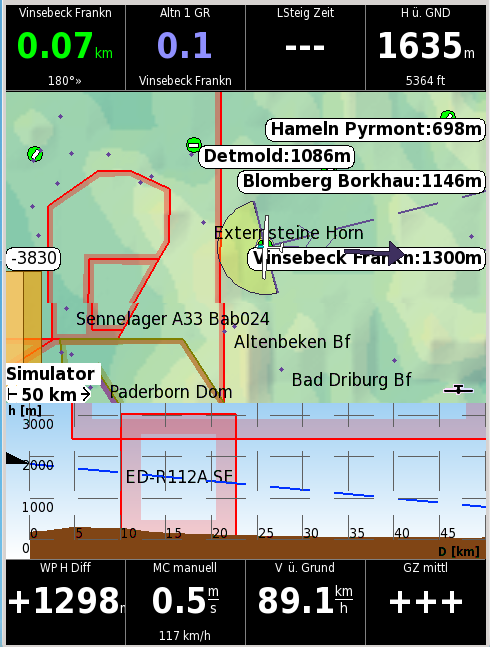
\includegraphics[angle=0,width=0.75\linewidth,keepaspectratio='true']{figures/plain.png}
\end{center}

Die  \textsf{XCSoar} Anzeige besteht aus mehreren Teilen:
\begin{description}
\item[\p{Kartenanzeige}] Die größte Fläche des Bildschirmes wird vom GPS-moving map beansprucht.
Wichtige Symbole, welche Informationen des Segelflugrechners darstellen, werden auf dieser Karte
eingeblendet (z.B. die Über/Unter Gleitpfad-Pfeile am linken Rand oder das Thermik-Höhenband).
Einige Icons und Textinformationen  erscheinen  (bei Bedarf) am unteren Rande des Displays,
welche über den Zustand des Rechners (verbunden mit GPS, Kurbelmodus, Endanflugmodus) etc.\  informieren.
%
\item[\p{{\InfoBox}en}] Eine bislang nur rechteckige Anordnung von sogenannten Info-Boxen, welche mit diversen Angaben, wie zum Beispiel Geschwindigkeit über Grund,
Höhe, MC Cready, geschätzte Zeit zum nächsten Wegpunkt usw. gefüllt ist, kann entweder am oberen und unteren Rand, rechts oder links,
oder auf der rechten Seite des Displays (im Quer- bzw. landscape-Modus) angezeigt werden. Bislang sind diese Anordnungen fix, in zukünftigen Versionen ist jedoch angestrebt, diese Infoboxen auch frei verschiebbar auf dem Display anordnen zu können.
%
hier werden diejenigen Werte, die der Benutzer vorher ausgewählt  hat und von \textsf{XCSoar} bzw. angeschlossenen Geräten ausgewertet werden, angezeigt.
%
\item[\p{Anzeigen}] Anzeigen stellen Instrumenten Displays dar (z.B. ein Vario). Alle Anzeigen sind optional und einige
haben lediglich informellen  Character, wenn \textsf{XCSoar} an ein unterstütztes Instrument angeschlossen ist.
%
\item[\p{Button Beschriftungen and Menüs}] Hardware-Knöpfe und die Wippe des Gerätes, auf dem \textsf{XCSoar} läuft, können benutzt werden, um Menüs bzw.\ Hauptmenüs aufzurufen, welche typischerweise den Hardwareknöpfen und /oder der Wippe fix zugeordnet sind. Dies erlaubt mitunter einen schnelleren Zugriff als das Bedienen allein des berührungsempfindlichen Bildschirmbereiches ("TouchScreen").
Falls das entsprechende Gerät über einen solchen TouchScreen verfügt (nahezu alle bis auf \al), können alle Menüs auch
hierüber geöffnet und bedient werden. Diese Buttons sind in schwarzem Text auf hellgrünem/grauen Hintergrund gestaltet.
%
\item[\p{Status Meldungen}] Hinweise zum Status des Fluges und auch des Flugzeuges  (z.B.\ Annäherung an einen Luftraum, vergessenes Fahrwerk, Startbestätigung bei Überfliegen der Start/Ziellinie etc\dots ) wird in einer Textbox  über dem Bildschirm eingeblendet.
Dieser Status Meldungen werden angezeigt, um detaillierte, wichtige Informationen zu geben, wenn gewisse, zum Teil konfigurierbarer Ereignisse, auftreten.
%
\item[\p{Dialog Fenster}] Die -größeren- Dialogfenster enthalten normalerweise Grafiken und Buttons. Diese werden verwendet, um dem Piloten  detaillierte Daten bezüglich Wegpunktdetails, Statistik und Analyse des bisherigen Fluges, Polaren etc\dots  zu übermitteln.

\item[\p{Hauptmenü}] das Hauptmenü wird entweder über einen Doppelklick auf die Bildschirmoberfläche oder aber über Gesten \gesture{Runter - Hoch} aufgerufen.

   Wenn die erscheinenden Buttons nicht innerhalb einer gewissen (einstellbaren) Zeit  betätigt  werden, verschwinden sie von sich aus wieder, um die Kartendarstellung des weiteren Fluges nicht zu behindern.
\end{description}

Die Bedienung von \textsf{XCSoar} ist auf verschiedene Wege möglich:

\begin{itemize}
\item Anklicken eines speziellen Kartenelements
\item Anklicken einer InfoBox und anschließend den Bildschirmmenüs
\item Benutzen einer "Geste", z.B. Zeichnen eines Striches von links nach rechts auf dem TouchScreen
 (siehe dazu Kap.~\ref{sec:gestures} weiter unten).
\item "Verschieben" (dragging) des Bildschirms (berühren und verschieben auf dem TouchScreen unter Fingerdruck).
\item Drücken der Hardware-Knöpfe des  Gerätes.
\item Drücken der Wippe des Gerätes.
\item Drücken  oder Schalten  an einem an \textsf{XCSoar} angeschlossenen Gerät.
\end{itemize}

Je nachdem, welcher Hardware bzw.\ welches Gerät mit \textsf{XCSoar}  benutzt wird, stehen nicht alle dieser Methoden zur Verfügung. Die Belegung der jeweiligen Hardware-Knöpfe können daher unterschiedlich sein.

Bei der \textsf{PC}-Version von \textsf{XCSoar} ist das Anklicken eines Bildschirmelements es mit der Maus identisch der Berührung mittels Touchscreen.

Da der \al nicht über einen TouchScreen verfügt, ist hier die Belegung der Menüs und Elemente grundlegend anders und wird über die dort vorhanden Hardware-knöpfe und Drehgeber vorgenommen.

 \newpage
 \section{Grundlegende Layouts von\textsf{XCSoar}}
 \textsf{XCSoar} läßt sich von der Oberfläche her extrem flexibel anpassen, je nach Geschmack des Benutzers. 
 Ich will hier lediglich vier unterschiedliche Darstellungen zeigen, welche allesamt im Konfigurationsmenü eingestellt werden können. 

 \begin{center}
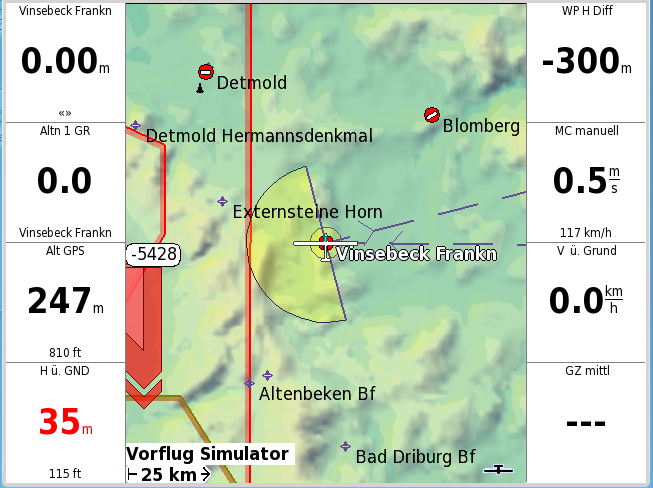
\includegraphics[angle=0,width=0.45\linewidth,keepaspectratio='true']{figures/map-outfit2.png}\quad
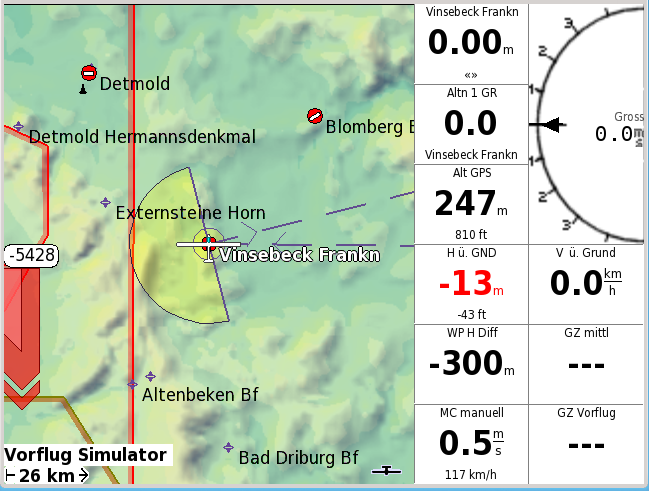
\includegraphics[angle=0,width=0.45\linewidth,keepaspectratio='true']{figures/map-outfit3.png}\vspace{1em}
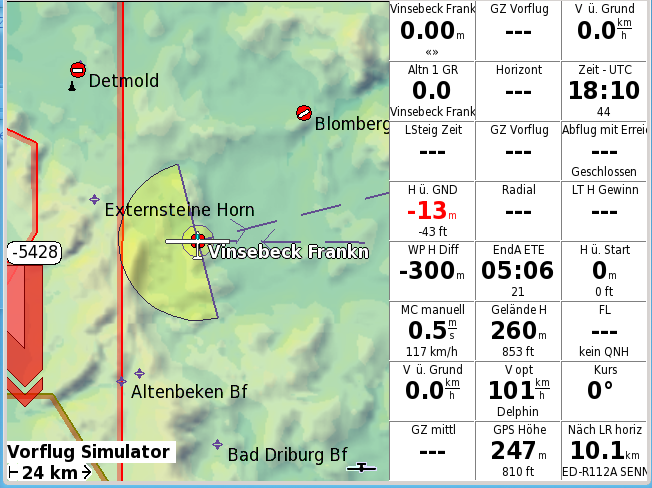
\includegraphics[angle=0,width=0.45\linewidth,keepaspectratio='true']{figures/map-outfit4.png}\quad
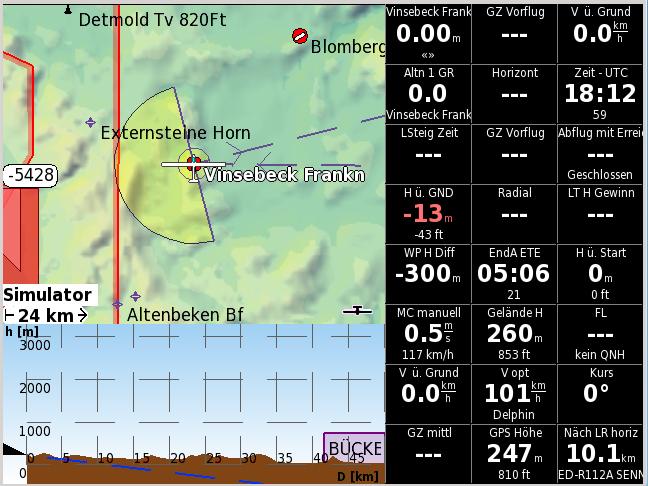
\includegraphics[angle=0,width=0.45\linewidth,keepaspectratio='true']{figures/map-outfit5.png}\vspace{1em}
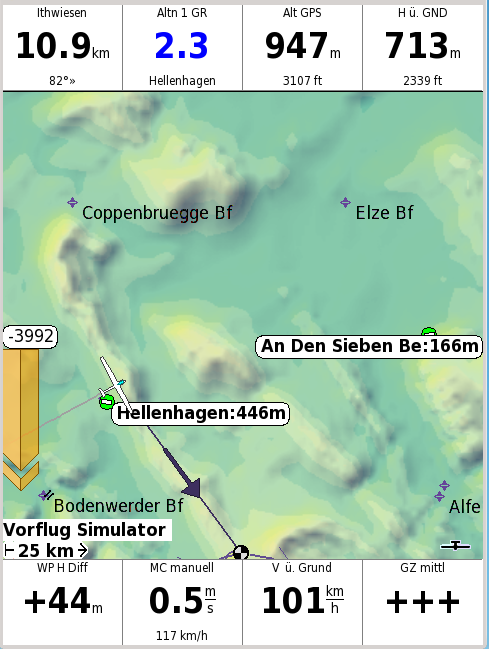
\includegraphics[angle=0,width=0.45\linewidth,keepaspectratio='true']{figures/map-outfit1.png}\quad
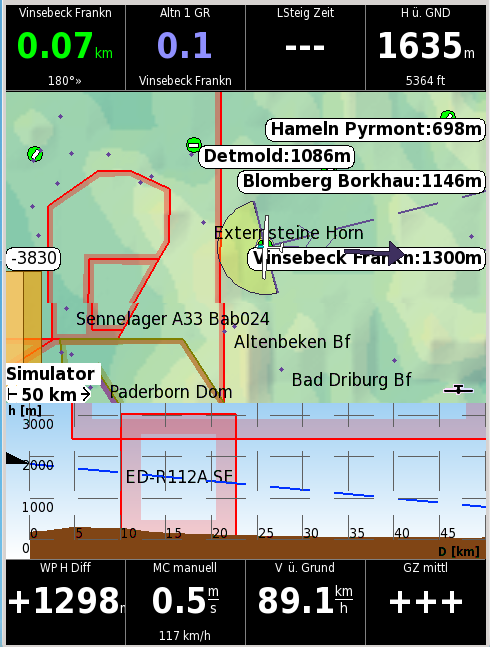
\includegraphics[angle=0,width=0.45\linewidth,keepaspectratio='true']{figures/map-outfit6.png}
\end{center}
Ob hochkant, quer, quadratischt schwarz oder weiß, mit Vario oder ohne, auch komplett ohne Infoboxen - alles möglich.
Die Einstellungsvarianten mögen auf den ersten Blick schier unübersichtlich sein, innerhalb weniger Tage oder Flüge jedoch habt ihr mit Sicherheit Eure Lieblingskonfiguration gefunden.


Ich beschränke mich in diesem Handbuch  grundsätzlich auf die hocjhkant (Portrait) Darstellung, da fats alle älteren PDA nur für diese geeignet erscheinen. Bei moderneren Android Geräten mag dies anders ein. Kann ja jeder machen wie er lustig ist.
   
 \newpage\section{Button-Beschriftungen und -Menüs}
Das Button-Menü besteht aus einem Satz von Buttons und Menüs und ist wird -bis auf die o.g. genannten Ausnahmen- mittels des TouchScreens aufgerufen (Doppelklick auf die berührungsempfindliche Oberfläche).

Die Benutzung der Buttons und des Button-Menüs  stellt die bevorzugte Art der Interaktion mit \textsf{XCSoar} dar.

\begin{center}
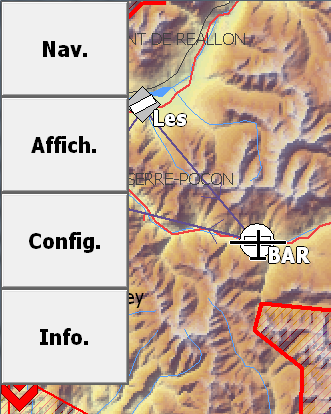
\includegraphics[angle=0,width=0.75\linewidth,keepaspectratio='true']{figures/buttonmenu.png}
\end{center}

\subsection*{Grundlegende Info zur Bedienoberfläche}
Das Menü ist in vier Hauptgruppen mit hoffentlich aussagekräftigen Namen (\textbf{Nav}, \textbf{Anzeige}, \textbf{Konfig.} und \textbf{Info}) unterteilt, welche diverse Untermenüs besitzen. Das spezielle Layout hängt vom jeweils benutzten Gerät ab und kann ebenso vom Bediener angepaßt werden. \textbf{Beenden} und \textbf{Abbrechen} vertseht sich wohl von slebst. 

 \textsf{XCSoar} kann ebenso über an das Gerät angeschlossene externe Eingabegeräte wie Joysticks, externe Tastaturen, game-pads und Multifunktionsgriffe bedient werden. Die hierüber aufzurufenden Funktionen können in großem Rahmen eben falls frei konfiguriert  werden.


Beim  \al  gibt es vier Hauptmenüs, welche durch Drücken auf die Knöpfe an der linken Seite aufgerufen werden können. 

Sowie ein Menü aktiviert wurde, erscheinen Untermenüs mit entsprechenden Beschriftungen über der unteren Druckknopfreihe. 
Hiermit kann man sich dann durch die entsprechenden Menüs und Funktionen weiter hindurchmanöverieren. 
Auf der letzten Seite eines jeden Menüs erscheint wieder der Menü-Knopf, mit dem man schließlich wieder auf den 
Bildschirm zurückkommt und alle Menüs verschwinden wieder vom Schirm. 
 


Auf dem \textsf{PC} werden diese Hauptmenü-Funktionen über die Ziffertasten 1, 2, 3 und  4 aufgerufen. Die Tasten 6, 7, 8, 9 und  0 sind dabei mit den
entsprechenden Untermenü-Funktionen der horizontal bzw.\ vertikal angeordneten Reihe von Buttons  zugeordnet.

Bei der PDA Version können die Hauptfunktionen direkt über die vier Hardware-Knöpfe über/unter (je nach Gerät) neben der Schaltwippe aufgerufen werden.

Falls ein Menü aufgerufen wird und nach einer gewissen Zeit keinerlei Eingabe mehr erfolgt, wird das angewählte Menü automatisch wieder geschlossen.  Diese Verzögerungszeit ist frei definierbar.  Auf dem \textsf{PC} kann die ESC- Taste hierzu benutzt werden, beim  \al wird hierzu der PWR/ESC- Knopf benutzt.

Wenn die Menü-Buttons grau erscheinen, ist die entsprechende Funktion nicht verfügbar.

So ist zum Beispiel der Button \textcolor{white}{\button{Wegpunkt Liste}} grau hinterlegt und die Schrift weiß gefärbt, falls keine Wegpunkt-Liste (besser: keine Wegpunkt-Datei) zur Verfügung steht oder geladen ist.

Einige der Menü-Buttons sind mit dynamischem Text versehen, d.h. die Beschriftung ändert sich entsprechend des Zustandes (gedrückt/nicht gedrückt). Folgendes Verhalten ist hierbei grundlegend festgelegt:


\textbf{Die Beschriftung des Buttons zeigt an,\textcolor[rgb]{0.72,0.03,0.20}{ was geschehen wird}, wenn er \achtung gedrückt wird, er zeigt also nicht den aktuellen Zustand an!}\index{Schaltflächen!Anzeigeverhalten}

Wird zum Beispiel auf der Schaltfläche  \button{MC Auto} angezeigt, dann wird ein Klick hierauf   'Auto
McCready' einschalten, und die Beschriftung wechselt zu  \button{MC Manuell}.
In der unten aufgelisteten Liste sind die Standard Beschriftungen aufgeführt.

\subsection*{Übersicht der Menüs}\index{Menü!Übersicht}
Im Folgenden wird beschrieben, wie das Menü allgemein aufgebaut ist.
Dies gilt für alle Plattformen (\textsf{PC}, Android, \al PDA, etc\dots

Die entsprechenden Funktionen werden in nachfolgenden Kapiteln ausführlicher beschrieben.

\textsf{\al}:

Die vier primären Menübuttons (Hauptmenü) werden beim \al durch Drücken der vertikal angeordneten Knöpfe an der linken Seite wie folgt von unten nach oben aktiviert:

\begin{jspecs}
\item[\button{Nav}]      Kontrolle und Einstellungen bezüglich Navigation, hauptsächlich gedacht für Tasks (Aufgaben).
\item[\button{Anzeige}]  Einstellungen der Anzeige von \textsf{XCSoar}
\item[\button{Konfig.}]  Konfiguration von \textsf{XCSoar}, angeschlossener Geräte,
                                      Einstellungen während des Fluges (Wind, Ballast, MC etc.\
\item[\button{Info}]     Aufruf diverser Informations Fenster,  Checkliste, Lufträume, Wetter etc.\
\end{jspecs}

In der \textsf{\textsf{PC}}-Version werden hierfür die Tasten  1, 2, 3 und 4 verwendet.

\subsection*{Navigationsmenü (Nav)}\index{Navigations-Menue}\index{Menü!Navigation}
\jindent{\bmenus{Aufgabe}}{ Blendet Aufgabenverwaltung und - Rechner ein. }
\jindent{\bmenut{Vorheriger}{Wegpunkt}}{ Wählt den vorherigen Wegpunkt innerhalb der Aufgabe an. }
\jindent{\bmenut{Nächster}{Wegpunkt}}{ Wählt den nächsten Wegpunkt innerhalb der Aufgabe an.}
\jindent{\bmenut{Wegpunkt}{Liste}}{ Zeigt die Wegpunkt - Auswahl an.}
\jindent{\bmenus{Alternativen}}{ Zeigt eine  Schnellauswahl-Liste der nahesten landbarer und erreichbarer Plätze in der Nähe an.}
%
%
%
\jindent{\bmenut{Aufgabe}{Abbruch}}{ Bricht die Aufgabe ab und geht über in den "Lustflug-Modus".}
\jindent{\bmenus{Gehezu}}{ Blendet die Wegpunkt-Auswahl 1ein und aktiviert den "Gehezu"-Modus für den ausgewählten Wegpunkt. }
\jindent{\bmenus{Target}}{ Zeigt den Target-Dialog. Entscheidend für AAT-Aufgabe. Hier können u.a. AAT-Wegpunkte verschoben werden. }
\jindent{\bmenut{Wegpunkt}{Details}}{ Blendet Details zum aktuell gewählten Wegpunkt ein.}


\subsection*{Anzeigemenü (Anzeige)}\index{Anzeige-Menue}\index{Menü!Anzeige}
\jindent{\bmenut{Zoom}{herein}}{ Zoomt die Karte herein (Kartenausschnitt kleiner, mehr Details. }
\jindent{\bmenut{Zoom}{heraus}}{ Zoomt  die Karte heraus (Kartenausschnitt größer,weniger Details. }
\jindent{\bmenut{Zoom}{Auto}}{ Schaltet zwischen  Zoom Auto und  Zoom Manuell hin und her. }
\jindent{\bmenut{Marke}{Setzen}}{ Setzt einen Marker der aktuellen Position auf der Karte. }
\jindent{\bmenut{Verschieben}{Ein}}{ Schaltet den Verschiebe-Modus der Karte ein. }
%
%\jindent{\bmenut{Beschriftungen}{Aufgaben\& Landeplätze}}{ Blendet die Beschriftungen der Wegpunkte innerhalb Aufgaben ein oder aus.. }
\jindent{\bmenud{Beschriftungen}{Aufgaben}{\& Landeplätze}}{ Blendet die Beschriftungen der Wegpunkte innerhalb Aufgaben ein oder aus.. }
\jindent{\bmenut{Spur}{Kurz}}{ Schaltet die Spur des bisherigen Fluges (kurz, lang, aus). }
\jindent{\bmenut{Gelände}{Aus}}{ Schaltet die Darstellung de Geländes auf der Karte ein oder aus. }
\jindent{\bmenut{Topo.}{Aus}}{ Schaltet die Topologie ein oder aus. }
\jindent{\bmenut{Info}{Auto}}{ Schaltet die Infoboxen (Kurbeln, AAT, Endanflug, Auto). }
%
%
%
\subsection*{Konfigurationsmenü (Konfig.\ )}\index{Konfig-Menue}\index{Menü!Konfig}
\jindent{\bmenut{MC}{$+$}}{ McCready größer. }
\jindent{\bmenut{MC}{$-$}}{ McCready kleiner. }
\jindent{\bmenut{MC}{Auto}}{ Schaltet zwischen McCready Auto oder und McCready manuell. }
\jindent{\bmenut{Flug}{Einstellungen}}{ Zeigt das Flug-Einstellungsfenster  (Mücken, Ballast, QNH). }
\jindent{\bmenut{Wind}{Einstellung}}{ Ruft das Windeinstellungsmenü auf.}
%
%
%
\jindent{\bmenus{Vario}}{ Kontrolle des Vega - Varios, dies enthält ein Untermenü.  Nur wählbar, wenn auch ein Vega angeschlossen ist. }
\jindent{\bmenut{System}{Einstellungen}}{ Öffnet die \textsf{XCSoar}-System-Einstellungen. Hierunter liegen 21 weitere Dialogfenster zur kompletten Konfiguration \textsf{XCSoar}s. }
\jindent{\bmenut{Luftraum}{Einstellungen}}{ Öffnet den Luftraum-Dialog. }
\jindent{\bmenut{Logger}{Start}}{ Schaltet den internen \textsf{XCSoar}- IGC-Logger an oder aus.. }
\jindent{\bmenus{Wiedergabe}}{ Startet das Wiedergabe-Fenster aufgezeichneter Flüge. }
%
\jindent{\bmenut{Roh}{Logger}}{ Schaltet den NMEA-Rohdaten-Logger ein oder aus (nur benutzt zur Entwicklung/Debuggen von \textsf{XCSoar}). }
\jindent{\bmenus{NMEA}}{ Öffnet den NMEA (z.B. GPS-Anschluß) Dialog. }
\jindent{\bmenus{Flugzeug}}{ Öffnet den Dialog zur Eingabe von flugzeugspezifischen Details. }
%
%
%
\subsection*{Informations Menü  (Info)}\index{Info - Menue}\index{Menü!Info}
\jindent{\bmenus{FLARMRadar}}{ Öffnet das Flarm-Radar-Fenster (Nur, wenn Flarm angeschlossen und erkannt) }
\jindent{\bmenut{METAR}{TAF}}{ Zeigt das METAR/TAF Fenster. }
\jindent{\bmenut{Naher}{Luftraum}}{ Zeigt die Details des nächstgelegenen Luftraumes. }
\jindent{\bmenut{Check}{Liste}}{ Öffnet die Checkliste, falls vorhanden}
\jindent{\bmenus{Analyse}}{ Öffnet den Analyse/Statistik-Dialog. }
%
\jindent{\bmenus{Status}}{ Öffnet den Status-Dialog. }
\jindent{\bmenus{Wetter}}{ Öffnet das Wetter-Dialog-Fenster. }
\jindent{\bmenut{Team}{Code}}{ Einblendung des TEAM-Code Dialoges.}
\jindent{\bmenut{FLARM}{Details}}{ Öffnet das FLARM-Detail-Fenster.}
\jindent{\bmenus{Zentrierhilfe}}{ Öffnet die Zentrierhilfe.}
%
\jindent{\bmenus{Mitwirkende}}{ Zeigt Versionsnummer und eine Reihe der Mitwirkenden an \textsf{XCSoar} an. }
\jindent{\bmenut{Naher}{Wendepunkt}}{ Zeigt Details des nächst gelegenen Wegpunktes an. }
\jindent{\bmenut{Wiederhole}{Meldung}}{ Wiederholt die zuletzt ausgegebene Meldung \textsf{XCSoar}s. }
%
%
%
\subsection*{Variometer-Untermenüs (Vario) des Konfigurationsmenüs (Konfig.\ )  }
Die Funktionen dieses Menüs sind ausschließlich anwählbar, wenn das VEGA Vario als Gerät an \textsf{XCSoar} angeschlossen ist.
\begin{center}

\end{center}
\jindent{\bmenut{Airframe}{Switches}}{ Displays airframe switch values. }
\jindent{\bmenut{Setup}{Audio}}{ Adjusts volume of sounds produced by \textsf{XCSoar} as well as certain speech announcements by the Vega intelligent variometer. }
\jindent{\bmenut{Manual}{Demo}}{ Activates Vega variometer manual tone demo. }
\jindent{\bmenut{Setup}{Stall}}{ Opens Vega stall monitor setup dialog. }
\jindent{\bmenus{Accel}}{ }
\jindent{\bmenut{ASI}{Zero}}{ Zeros the airspeed indicator. }
\jindent{\bmenut{Accel}{Zero}}{ Levels/zeros the accelerometers. }
\jindent{\bmenus{Store}}{ Stores Vega settings to EEPROM. }
\jindent{\bmenut{Cruise}{Demo}}{ Activates Vega variometer cruise tone demo. }
\jindent{\bmenut{Climb}{Demo}}{ Activates Vega variometer climb tone demo. }
\subsection*{Verschieben-Untermenü des Anzeige-Menüs}
\jindent{\bmenut{Verschieben}{aus}}{ Schaltet Verschiebemodus aus. }
\jindent{\bmenut{Zoom}{herein}}{ Zoomt Karte herein. }
\jindent{\bmenut{Zoom}{heraus}}{ Zooms Karte heraus. }
\jindent{\bmenut{Naher}{Wegpunkt}}{ Zeigt das Wegpunkt-Detail Fenster, oder aber, falls die Karte verschoben wurde, das Wegpunkt-Detail Fenster zu jenem Wegpunkt, an dem sich das Fadenkreuz (sichtbar beim Verschieben, immer in der Mitte der Karte), befindet. }
\subsection*{Standard-Buttons}\index{Buttons!Standard}
Wenn keinerlei Menü aktiv ist, (der sog.\ \textsl{default-mode}) dann sind beim \al den horizontalen Knöpfen die folgenden Funktionen zugeordnet. In der oberen Reihe die \textsf{PC}-Tasten, in der unteren Reihe die \al-Tasten.
Unten die entsprechende Standard-Funktionsbelegung:
\begin{center}
\begin{tabular}{c c c c c}
 6 & 7 & 8 & 9 & 0 \\
 F5 & F6 & F7 & F8 & F9 \\
\smenut{Flug}{Einstellung} & \smenut{Task}{Calc} & \smenut{Task}{Edit} &
\smenut{Arm}{Advance} & \smenut{Marker}{setzen} \\
\end{tabular}
\end{center}

Wenn der ESC-Knopf des \al kurz gedrückt wird, erscheint die Beschreibung der Knöpfe.
Bei allen anderen Geräten / Plattformen wirken die cursor-Tasten wie folgt:


\begin{jspecs}\index{Buttons!\al}
\item[\p{Hoch Taste}] Zoom herein
\item[\p{Runter Taste}] Zoom hinaus
\item[\p{Links Taste}] Nächster InfoBox-Set
\item[\p{Rechts Taste}] Letzter InfoBox-Set
\item[\p{Enter}] Bestätigen/Löschen von Status-Mitteilungen oder aber Flarm-Meldungen unterdrücken, wenn diese erscheinen und keine Warnung aktiv ist
\end{jspecs}
Der Drehknopf des \al  ist im default-mode wie folgt belegt:


\begin{jspecs}
\item[\p{Äußerer Knopf gegen Uhrzeigersinn}] Zoom herein
\item[\p{Äußerer Knopf im Uhrzeigersinn}]  Zoom heraus
\item[\p{Innerer Knopf gegen Uhrzeigersinn}] (Nicht belegt)
\item[\p{Innerer Knopf im Uhrzeigersinn}] (Nicht belegt)
\item[\p{Drücken des Knopfes}] Bestätigen von Status Meldungen und Luftraum Warnungen/Hinweisen
\end{jspecs}




In Dialog Fenster sind den Drehknöpfen des \al folgende , Cursor-ähnliche Funktionen zugewiesen:


\begin{jspecs}
\item[\p{Äußerer Knopf gegen Uhrzeigersinn}] Cursor hoch
\item[\p{Äußerer Knopf im Uhrzeigersinn}] Cursor runter
\item[\p{Innerer Knopf gegen Uhrzeigersinn}] Cursor links
\item[\p{Innerer Knopf im Uhrzeigersinn}] Cursor rechts
\item[\p{Drücken des Knopfes}] Bestätigen/OK-Taste
\end{jspecs}


Beim \al können alternativ die folgenden Knöpfe entlang des Gehäuserandes für die Navigation innerhalb von Dialogen benutzt werden:

Der F4-Knopf kann innerhalb von Dialogen als alternative zur ENTER-Taste (Drücken des Drehknopfes) benutzt werden.
F6 und F7 können benutzt werden um die nächste bzw.\ letzte Seite innerhalb von Dialogseiten anzuwählen.
\subsection*{Dynamische Menübeschriftungen}\index{Menü-Beschriftungen}
Die meisten Menüs haben dynamische Beschriftungen, um klarer hervorzuheben, welche Aktion diesem Menü zugeordnet ist, wenn der jeweilige Button bedient wird.

Falls ein Menü oder Button grau hinterlegt ist, so steht diese Funktion zum jeweiligen Zeitpunkt \emph{nicht} zur Verfügung und ein Klick darauf bewirkt gar nichts.

Folgende Konvention zur Belegung bzw. Beschriftung der Buttons und Menüs wird  innerhalb \textsf{XCSoar} verwendet:

Beispiel:

Erscheint z.B.:  "Licht an'' als Beschriftung, so  wird das Licht \emph{an}geschaltet und  es erscheint dann als Beschriftung z.B. "Licht aus".  Ein erneute Drücken schaltet dann das Licht wieder \emph{aus}.

Stehen mehrere Funktionen eines Knopfes zur Verfügung, (z.B.\ zusätzlich noch "Licht gedimmt", dann kann durch Drücken des Buttons zyklisch durch diese Funktionen durchgewählt werden:


\begin{center}
"Licht an'' $\rightarrow$ "Licht gedämmt'' $\rightarrow$ "Licht aus'' $\rightarrow$" Licht an" $\rightarrow$ "Licht gedämmt'' und so weiter\dots
\end{center}

Eine Auswahl von dynamisch beschrifteten Buttons ist als Beispiel hier unten aufgelistet:

\begin{description}
\item[\button{Nächster Wendepunkt}]
  Grau, wenn keine  Aufgabe aktiv ist, oder aber wenn der nächste Wendepunkt gleich dem Zielpunkt (also dem letzten Wegpunkt) ist.

 Wenn der nächste Wegpunkt gleich dem Ziel ist, dann erscheint " Wendepunkt Ziel''.
\item[\button{Letzter Wendepunkt}]
  Grau, wenn keine  Aufgabe aktiv ist, oder aber wenn der vorherige Wendepunkt gleich dem Startpunkt ist und es keine verlegten Startpunkte gibt. .

  Falls verlegte Startpunkte vorhanden sind und der aktive Wendepunkt gleich dem Start ist, wird "zyklischer Start" angezeigt um aus den diversen Startpunkten einen entsprechenden auszuwählen.

Wenn der aktive Wegpunkt gleich dem ersten Wegpunkt nach dem Start ist, dann erscheint  "Wendepunkt Start''.
\item[\button{Beschriftungen}]
Angezeigt wird hierbei folgendes: " Beschriftung Aufgabe \& Landeplätze", "Beschriftung Keine", Beschriftung Alle.

\item[\button{Nächster Wendepunkt}]
 Grau,  wenn keine Wegpunkt-Datenbank hinterlegt ist.
 \item[\button{Vorheriger Wendepunkt }]
  Grau,  wenn keine Wegpunkt-Datenbank hinterlegt ist.
\item[\button{Wegpunktliste }]
  Grau,  wenn keine Wegpunkt-Datenbank hinterlegt ist.
\end{description}

\section{{\InfoBox}en}\index{InfoBoxen}

\textsf{XCSoar} stellt nahezu alle wichtigen Werte mittels  sog.\  {\InfoBox}en dar. 


Diese {\InfoBox}en können zu InfoBoxfenstern (s.u.) zusammengestellt werden und mit
\emph{gewissen Einschränkungen \footnote{In Planung ist, in kommenden Versionen einige oder alle 
InfoBoxen auch frei verschiebbar darzustellen}} beliebig auf dem Bildschirm plaziert werden. 
Die Informationen, welche in den  {\InfoBox}en dargestellt werden sollen,  können aus einer großen Anzahl (gelistet im Kapitel~\ref{cha:infobox}) ausgewählt werden.

Die mögliche Anzahl und das Layout \sketch{figures/infoboxes.png}der {\InfoBox}en  hängen von der Ausrichtung des Bildschirmes und von der Größe bzw. Auflösung des Bildschirms des entsprechende Gerätes ab. 

Für ein typisches 320$\times$240 Pixel-Display (Pocket-\textsf{PC} im "Hochkant"-Modus) stehen jeweils vier {\InfoBox}en am oberen und unteren Rand des Displays zur Verfügung. 
Im Querformat, sind neun {\InfoBox}en an der rechten Seite des Displays vorgesehen. Siehe Bild unten:


\subsection*{Bildschirmanzeige-Modi / InfoBox-Seiten}\index{InfoBoxen!Seiten}

\textsf{XCSoar} gestattet dem Piloten einen ganzen Satz an individuell belegten Infobox-Seiten zu erstellen.
Dies dient dazu, bestimmte Werte, die zum Beispiel vor allem beim Kurbeln  benötigt werden übersichtlich und schnell darzustellen.
Ein anderer Satz an Infoboxen könnte zum Beispiel für den Endanflug oder aber während Wettbewerbsaufgaben erstellt und angezeigt werden.

\textsf{XCSoar} so kann so konfiguriert werden, daß es automatisch auf die jeweilige Seite umschaltet, oder aber ein manuelles Umschalten erforderlich ist. Der Name der aktuellen InfoboxSeite kann ganz unten links am Rande der Karte abgelesen werden.

Es ist ebenfalls möglich, überhaupt keine Infoboxen auf der Karte darzustellen, in diesem Fall erscheint ausschließlich die Landkarte mit Topologie bzw. Karte auf dem Bildschirm.

Um durch die diversen Infobox-Seiten hindurch zu schalten, kann der TouchScreen benutzt werden
\gesture{Rechts oder Links}. 

Auf PDA ist es ebenfalls möglich,  mittels der Schaltwippe  (nach rechts oder links) durch die diversen Seiten hindurch zu schalten.

\subsection*{Ändern von  {\InfoBox} Werten}\index{InfoBoxen!Werte Ändern}
(Dieser Abschnitt ist ausschließlich gültig, wenn ein Touchscreen oder eine Maus zur Verfügung steht.)

Einige {\InfoBox}-Werte können durch drücken auf den Touchscreen oder aber mit der Maus vom Piloten geändert.
Hierzu müssen die entsprechenden {\InfoBox}en  \emph{langanhaltend} gedrückt werden.
Ein kurzes Klicken reicht dazu nicht.  Nach dem loslassen erscheinen weitere {\InfoBox}en:

\begin{description}
\item[\button{Edit}]
Erlaubt dem Piloten den Wert der entsprechenden {\InfoBox} zu ändern (zum Beispiel den McCready Wert).

\item[\button{Setup}]
hiermit kann das Verhalten der entsprechenden {\InfoBox} geändert werden. Beispielsweise kann der McCready Wert von Auto auf Manuell geschaltet werden.
Weiterhin kann hier durch Klicken auf  \button{Setup InfoBox} innerhalb dieser {\InfoBox}  eine Liste mit allen verfügbaren {\InfoBox}en dargestellt werden, welche an dieser Stelle der InfoboxSeite erscheinen soll. hierzu erscheint ein Button "Infobox Einstellungen"

\item[\button{Schließen}] Na, was wohl\dots
\end{description}

{\InfoBox}en, deren Werte geändert werden können, sind zum Beispiel der McCready wert, oder aber die Windgeschwindigkeit und Richtung. Im Simulator-Modus, zählt auch die Höhe, sowie die Übergrundgeschwindigkeit hierzu.

\subsection*{Ändern von {\InfoBox}en}
{\InfoBox}en können entweder über das Konfigurationsmenü geändert werden 
\menulabel{\bmenut{Konfig.}{2/3}\blink\bmenus{System}} (ausführlich beschrieben in Kap.\ref{sec:interface-appearance})
oder durch einen länger anhaltenden Druck auf die entsprechende  {\InfoBox}, welche geändert werden soll.
 In diesem Fall erscheint ein Dialog mit allen verfügbaren {\InfoBox}en, aus denen die \menulabel{~~\button{Aussehen}\blink\button{Infobox Sets}}gewünschte ausgewählt werden kann.
 

\section{Status Meldungen}
Status-Meldungen erscheinen im oberen Bereich des Bildschirms über die gesamte Kartenbreite und sind für die kurzfristige Anzeige von Meldungen gedacht. Nach einer einstellbaren Zeit verschwinden diese Meldungen von selbst. Verschiedene Meldungen können mit verschiedenen Anzeigezeiten belegt werden.

Zusätzlich können bestimmte Statusmeldungen mit einer Bestätigungs-Aufforderung versehen sein.
Die Bestätigung erfolgt entweder durch Drücken des Drehknopf es beim \al, Drücken der Statusmeldung auf dem TouchScreen oder aber Anklicken mit der Maus (\textsf{PC}).  Zusätzlich können benutzerdefinierte Buttons definiert werden, welche die zuletzt gezeigte Status Meldung wiederholt.

Hier ein paar typische Statusmeldungen:
\begin{itemize}
\item Luftraum Warnungen
\item Meldungen der Programmes an sich zur Optik wie z.B. Ändern des Anzeigemodus (hochkant/quer, Auflösung)
\item Meldungen des Segelflugrechners wie z.B. Start, Startlinie überflogen, Erreichen eines Wendepunktes etc\dots  )
\end{itemize}

Beachte, daß Statusmeldungen nicht erscheinen, während ein Dialog auf dem Bildschirm erscheint. Diese Meldung wird gespeichert und erst dann angezeigt, nachdem das Dialogfenster verlassen wurde.

\section{Dialog Fenster}\label{sec:dialog-windows}

\textsf{XCSoar} verfügt über etliche Dialogfenster, welche aufgerufen werden können um zusätzliche Informationen darzustellen. Weiterhin werden Dialogfenster benutzt, um zum Beispiel Konfigurationseinstellungen vorzunehmen, Aufgaben (tasks) zu erstellen, usw.\

Manche Dialoge zeigen einfach nur Informationen und fordern keinerlei Aktion des Piloten, andere dagegen zeigen Felder, deren Werte geändert werden können und erfordern eine Eingabe vom Piloten oder einfach nur das Drücken eines anderen Buttons.

Ein vom \textsf{PC} gewohnte Cursor erscheint über dem aktiven Button oder Datenfeld.
Wenn die hoch/runter Tasten gedrückt werden (oder aber der äußere Drehknopf auf dem \al), rückt der Cursor zum nächsten bzw. vorherigen Listenelement.

Für lange Listenelemente und scrollbaren Text, werden die Hoch- und Runter-Tasten zur Navigation durch den Text benützt, und die links- und Rechts-Tasten bewegen jeweils eine komplette Seite vor oder zurück.

Für die PDA und \textsf{PC}-Version, können solche Listen geändert werden, indem das jeweilige Listenelement angeklickt wird.
Wenn ein Listenelement angewählt wurde, ist ein weiterer Klick gleichbedeutend mit der Enter-Taste bzw. einem O.K.

Durch Drücken der rechts/links Tasten Innerhalb eines gewählten Listenelement des (bzw. Drehen des inneren Knopfes auf dem \al) werden die Werte dieses Listenelement des geändert. Durch Drücken der OK- bzw. Enter-Taste dies (oder Drücken des Drehknopf das auf dem Alter) wird der Button aktiviert oder ein Listenelement aus einer Liste ausgewählt.

Dialoge werden typischerweise vom Button Menü gestartet. Viele der Dialog Fenster haben mehrere Seiten mit Information, und sind innerhalb \textsf{XCSoar} immer gleich zu bedienen:

Die \button{$<$} und \button{$>$} Buttons wählen die vorherige bzw. die nächste Seite aus und der
\button{Close} Button dient  zum Verlassen des Dialogs. (Gleichbedeutend ist die ESC-Taste auf dem \textsf{PC} bzw. die ESC/PWR-Taste  auf dem \al.)

Die Dialogfenster müssen explizit vom Piloten geschlossen werden. Wenn ein Dialogfenster geöffnet ist, bleibt es so lange geöffnet, bis der Dialog geschlossen wird. In manchen Dialogfenstern werden bestimmte  Werte nicht dargestellt, sofern sie irrelevant sind. (so zum Beispiel die Delta-Zeit einer AAT-Aufgabe, wenn keine AAT-Aufgabe geflogen wird).


Eine Liste der wichtigsten Dialoge ist hier aufgelistet:
\begin{description}
\item[\p{Flug Einstellung}] Einstellung des QNH, der Polare, Mückenbeladung, Wasserballast
\item[\p{Wind Einstellung}] Einstellungen des Windes (Richtung, Stärke und Art der Berechnung )
\item[\p{Wegpunkt Details}] Details zu Wegpunkten wie Peilung (Bearing), Höhe, Frequenz (falls vorhanden), Sonnenuntergang  etc\dots
\item[\p{Wegpunkt Auswahl}] Auswahl eines Wegpunktes aus der Datenbank
\item[\p{Analyse}] Mehrere Seiten mit analytischen Details zum bisherigen Flugweg (Strecke, mittleres Steigen, echte, erflogene Polare u.v.m.)
\item[\p{Status}] Dieser Dialog bringt eine Zusammenfassung der aktuellen Situation/Konfiguration  des Flugzeuges, des Systems, der Aufgabe von Staat und Zeiten der Aufgabe.
\item[\p{Checkliste}] Eine Checkliste, welche vom Piloten selber erstellt werden kann und mehrere Seiten umfassen darf
\item[\p{Konfiguration}] Konfiguration von  \textsf{XCSoar} und angeschlossenen Geräten
\item[\p{Luftraum}] Konfiguration und Darstellung der Farben und Erscheinung von Lufträumen
\item[\p{Luftraum Filter}] Filter für die Lufträume. Ein- und Ausblenden von bestimmten lufträumen sowie die Bestätigen der Luftraumwarnungen.
\item[\p{Team Kode}] Einstellungen und Übermittlung von Koordinaten für den Teamflug
\item[\p{NMEA}] Einstellungen für die Schnittstellen externer Geräte z.B.  andere Segelflugrechner,  logger, \fl etc.).
\item[\p{Flugzeug Details}] Erlaubt auf einfache Weise flugzeugspezifische Einstellung wie z.B.\ Polare, Ballast, Flügelfläche oder DMST-Index aus voreingestellten Listen.
\end{description}

Diese Dialoge werden in nachfolgenden Kapiteln behandelt werden. Ausgenommen hiervon sind der Checklisten-, der Status-  und der Texteingabe-Dialog, welche hier unten im Anhang behandelt werden.


\subsection*{Checklisten Dialog}\index{Checkliste}

Der Checklisten-Dialog ist gedacht, um mehrere Seiten von Erinnerungen 
\menulabel{\bmenut{Info}{1/3}\blink\bmenut{Check}{liste}} und 
frei definierbarem Text des Piloten aufzunehmen. 

Die typische Anwendung hierfür ist eine Checkliste vor dem Start. Diese Checkliste kann Dinge enthalten wie z.B.:
Täglicher Check, Vorflugcheck, Außenlandungscheck, Pinkeltüten Einpacken, Erinnerung an Treibstoff, 
\sketch{figures/checklist.png}
Klappen beim Start verriegelt diverse laberfrequenzen usw.\ je nach Gusto des Piloten.  

Mit  \button{$<$} und \button{$>$} Buttons  können die jeweils nächsten Seiten angewählt werden.

Der Aufbau der kleinen Textdatei \verb|xcsoar-checklist.txt| ist im Kap.~\ref{sec:checklist-file} beschrieben. 


\subsection*{Status Dialog}
Der Statusdialog ist ein Dialog mit mehreren Seiten, welcher eine Übersicht über \menulabel{\bmenut{Info}{2/3}\blink\bmenus{Status}}das Flugzeug, das System, die Aufgabe, Regeln zur Aufgabe und Zeiten darstellt. 

\textbf{Achtung!}

Bitte beachtet, daß die Werte in diesem Dialog nicht aktualisiert werden, während die Seite dargestellt wird.
Das bedeutet, daß Positionen, Zeit, usw.\ nicht aktualisiert werden. 

Um die aktualisierten Werte dieser Seite zu betrachten, ist es notwendig diesen Dialog zu schließen und erneut zu öffnen!  

\begin{description}
\item[\button{Flug}]Zeigt die aktuelle Position \sketch{figures/status-aircraft.png}des Flugzeuges (Breiten - und Längengrad), den maximalen Höhengewinn, den nächstgelegenen Wegpunkt, dessen Entfernung  und die Peilung (bearing) dorthin.
\item[\button{System}] Zeigt den Status von angeschlossenen Geräten, Satellitenempfang,  Batterielevel
\item[\button{Aufgabe}] Anzeige von AAT-Zeit, Differenz-Zeit, Entfernungen und Aufgabengeschwindigkeit
\item[\button{Regeln}] Zeigt Gültigkeit des Abfluges, der Überquerung von Start/Ziellinien gemäß der eingegebenen Regeln der Aufgabe.
\item[\button{Zeiten}] Anzeige aller Zeiten wie z.B.: lokale zeit, GPS-zeit, Flugdauer, Start-  und Landezeit sowie den Sonnenuntergang.
\end{description}

\subsection*{Eingabe von Text} \label{sec:textentry}\index{Texteingabe}\index{Eingabe von Text}

Wie zu erwarten, ist der Texteingabedialog dazu da, Text einzugeben.
Benutzt und aufgerufen wird dieser Dialog von diversen Fenstern und anderen Dialogen, um z.B. Wegpunkte oder TeamCodes  einzugeben, Pilotennamen, Loggerdeklarationen u.v.m\dots
Im Kapitel~\ref{sec:status} wird auf die Details der oben beschriebenen Optionen eingegangen.

\menulabel{\bmenut{Konf.}{2/3}\blink\bmenus{System}} Zwei Möglichkeiten der Eingabe sind möglich und vorgesehen:  "Ranglisten"  und "Tastatur".
Voreingestellt ist "Tastatur"-welche für fast alle Endgeräte\menulabel{\quad\button{Aussehen}\blink\button{Sprache}} -bis auf \al sinnvoller und erheblich schneller und bequemer erscheint. Mit \button{Texteingabestil} wird der gewünschte Stil eingestellt.

Um die entsprechenden  Buchstaben einzugeben, werden im \textit{Ranglisten}-Stil die A+ und  A- Buttons benutzt, drücken auf  \button{$<$} bzw.\   \button{$>$} schiebt den Cursor an die entsprechenden Stelle.
 
\begin{center}
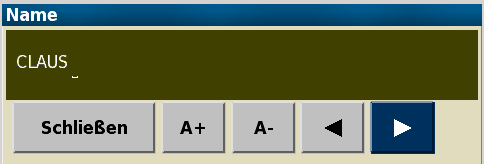
\includegraphics[angle=0,width=0.65\linewidth,keepaspectratio='true']{figures/textentry.png}
\end{center}

Um Text mit dem TouchScreen einzugeben, ist es sinnvoller  auf die "Tastatur"- bzw. Voreinstellung zu wechseln, einfach einen Buchstaben nach dem anderen mit der TouchScreen Tastatur eingeben (s.links).

In einigen Dialogen (z.B. beim Editieren und oder Eingeben \sketch{figures/textentry_keyboard.png}von Wegpunkten) schlägt \textsf{XCSoar} sofort den/die nächsten passenden Einträge aus der Datenbank vor bzw. unterdrückt nicht passende/nicht vorhandene Einträge, sodaß die Eingabe sehr schnell und komfortabel von sich geht.

Um den letzten Buchstaben zu löschen, drücke den  \button{$<-$} button.

Drücke auf  \button{Schließen} um die Eingabe zu übernehmen.

\section{Warntöne}\index{Warntöne}\index{Hinweistöne}

\textsf{XCSoar} erzeugt Geräusche für diverse Ereignisse, welche vom Bediener/Piloten  nach Belieben konfiguriert werden können.
Hierzu siehe~\ref{sec:status} für detaillierte Konfigurierung.

Wenn \textsf{XCSoar} an das VEGA-Variometer angeschlossen ist,  sendet \textsf{XCSoar} Kommando-Strings an das Subsystem des VEGA Sprachsystems, um von diesem Sprachausgaben und Warnungen erzeugen zu lassen, z.B.:

\begin{itemize}
\item Endanflug durch Gelände
\item Anfliegen/erreichen eines Wegpunktes
\item Luftraum Warnungen
\end{itemize}

\section{Bildschirmeinstellungen}

Es können einige Einstellungen der Bildschirmdarstellung und der Details auf \menulabel{\bmenut{Konfig.}{2/3}\blink\bmenus{System}}dem Bildschirm gewählt werden.  Der meistverwendet Punkt  ist hierbei wohl, ob die {\InfoBox}en weiß auf schwarz oder schwarz auf weiß - "invertierte Darstellung" genannt, dargestellt werden \menulabel{\quad\button{Aussehen}\blink\button{Anordnung}}sollen.  Einstellbar über \button{invertierte Infoboxen}. 

Die Einstellung der Helligkeit beim \al erfolgt entweder per \menulabel{\bmenut{Anzeige}{2/2}\blink\bmenus{Helligkeit}}Hardware gemäß des {\em \al User's Manual} oder aber wie links .  




\section{Hilfe System}
  Für die meisten Dialoge ist nun ein Hilfesystem vorhanden.
  Wenn eine Eigenschaft / ein Fenster \menulabel{\bmenus{Hilfe}} aufgerufen wurde, drücke auf den Hilfe-Knopf und eine entsprechender Hilfstext wird erscheinen, der die Auswahlmöglichkeiten  beschreibt. 

\section{Gestures}\label{sec:gestures}\index{Gesten}
Seit Version 6.0 unterstützt \textsf{XCSoar} auch sog.\  "Gesten".

Im Bild links wird angedeutet, wie man sich eine Geste vorzustellen hat. 
Es handelt sich hierbei um eine ganz normale Arbeitsweise, wie sie sie jeder kennt, der mit einem Touchscreen-Gerät
Für den normalen Bildschirm und für den \sketch{figures/gesture1.png} \fl-Bildschirm haben die Gesten unterschiedliche Bedeutungen, wie im  folgender Tabelle beschrieben wird. 
\newpage
 Wenn am Rande folgendes Icon \gesture{Hoch} erscheint, so bedeutet dies, daß für die beschriebene Funktion  die entsprechende Geste verfügbar ist. In diesem Falle  die Geste: ''Hoch''

%Eine Geste wird definiert als eine Bewegung von hoch, runter, rechts und links Bewegungen.
%Die Geste "LU"  z.B.\   steht hierbei für \gesture{Left-Up}.
%(Wenn am Rande der Seite das folgende Icon sichtbar ist, dann  stehen Gesten für die jeweilige Funktion zur %Verfügung.)

\textbf{Auf der Karte verfügbare Gesten:\index{Gesten! auf Karte}}

\begin{itemize}
 \item[\raisebox{-1em}{
\includegraphics[angle=0,width=0.1\linewidth,keepaspectratio='true']{figures/up.png}}] \p{Hoch}: Zoom herein 
 \item[\raisebox{-1em}{
\includegraphics[angle=0,width=0.1\linewidth,keepaspectratio='true']{figures/down.png}}] \p{Runter}: Zoom heraus 
 \item[\raisebox{-1em}{
\includegraphics[angle=0,width=0.1\linewidth,keepaspectratio='true']{figures/left.png}}] \p{Links}: Nächste InfoboxSeite 
 \item[\raisebox{-1em}{
\includegraphics[angle=0,width=0.1\linewidth,keepaspectratio='true']{figures/right.png}}] \p{Rechts}: vorherige InfoboxSeite 
\item[\raisebox{-1em}{
\includegraphics[angle=0,width=0.1\linewidth,keepaspectratio='true']{figures/du.png}}] \p{Runter-Hoch}: Menü anzeigen 
\item[\raisebox{-1em}{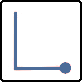
\includegraphics[angle=0,width=0.1\linewidth,keepaspectratio='true']{figures/dr.png}}] \p{Runter-Rechts}: Wegpunkt Dialog anzeigen 
\item[\raisebox{-1em}{
\includegraphics[angle=0,width=0.1\linewidth,keepaspectratio='true']{figures/rd.png}}] \p{Rechts-Runter}: Aufgabenverwaltung
\item[\raisebox{-1em}{
\includegraphics[angle=0,width=0.1\linewidth,keepaspectratio='true']{figures/urdl.png}}] \p{Hoch-Rechts-Runter-links}:  Verschiebemodus.  Dies geht aber auch  auch mit auf Android üblichem Spreizen oder Zusammenfahren von Zeigefinger und Daumen!
\end{itemize}


\textbf{Wenn das \fl-Radar auf dem Bildschirm aktiv ist, sind folgende Gesten verfügbar: }

\index{Gesten!FLARM Radar}
\begin{itemize}
\item[\raisebox{-1em}{
\includegraphics[angle=0,width=0.1\linewidth,keepaspectratio='true']{figures/up.png}}] \p{Hoch}: Zoom herein 
\item[\raisebox{-1em}{
\includegraphics[angle=0,width=0.1\linewidth,keepaspectratio='true']{figures/down.png}}] \p{Runter}: Zoom heraus 
\item[\raisebox{-1em}{
\includegraphics[angle=0,width=0.1\linewidth,keepaspectratio='true']{figures/left.png}}] \p{Links}: Letztes Ziel (Flugzeug)
\item[\raisebox{-1em}{
\includegraphics[angle=0,width=0.1\linewidth,keepaspectratio='true']{figures/right.png}}] \p{Rechts}: Nächstes Ziel (Flugzeug)
\item[\raisebox{-1em}{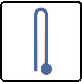
\includegraphics[angle=0,width=0.1\linewidth,keepaspectratio='true']{figures/ud.png}}]  \p{Hoch-Runter}: Aktiviere AutoZoom
\item[\raisebox{-1em}{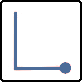
\includegraphics[angle=0,width=0.1\linewidth,keepaspectratio='true']{figures/dr.png}}] \p{Runter-Rechts}:  Öffne Detail-Fenster des gewählten Zieles (Flugzeuges)
\item[\raisebox{-1em}{
\includegraphics[angle=0,width=0.1\linewidth,keepaspectratio='true']{figures/rd.png}}] \p{Rechts-Runter}:  Öffnet die Aufgabenverwaltung
\item[\raisebox{-1em}{
\includegraphics[angle=0,width=0.1\linewidth,keepaspectratio='true']{figures/rl.png}}] \p{Rechts-Links}: Wechselt zur Anzeige von Werten wie z.B.\ Steigen, relativer Höhe etc.\ des angewählten Zieles (Flugzeuges) )
\end{itemize} 

%%%%%%%%%%%%%%%%%%%%%%
\chapter{Navigation}\label{cha:navigation}

In diesem Kapitel wird die ''moving map'' beschreiben, welche einen elementaren Bestandteil von \xc zur Navigation darstellt und heute selbstverständlich ist. 
Weiterhin werden hier die entsprechenden Elemente beschrieben, welche auf der Karte eingeblendet sind um die Navigation so schnell und einfach wie möglich zu machen.

\section{Elemente der Kartenanzeige}

\begin{maxipage}\centering
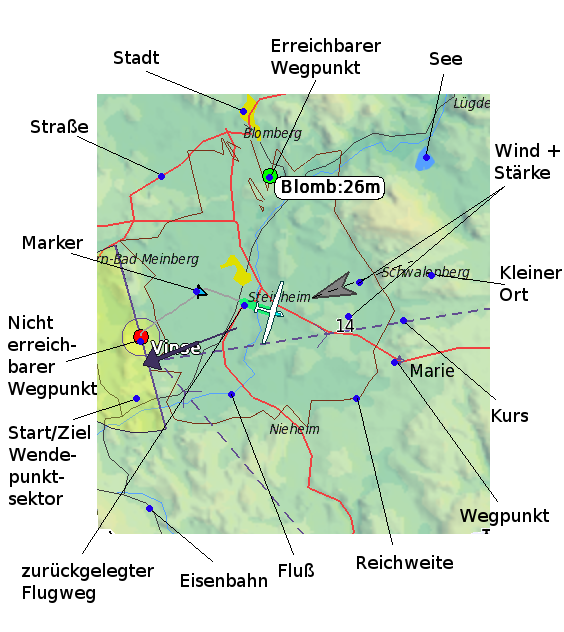
\includegraphics[angle=0,width=0.55\linewidth,keepaspectratio='true']{figures/fig-map.png}
\end{maxipage}

Die moving-map zeigt folgende Bestandteile:

\begin{enumerate}[itemsep=-0.25ex]
  \item Das Segelflugzeug Symbol
  \item Die Wegpunkte
  \item Die aktive Flugaufgabe (''task'')
  \item Den Kurs zum gewählten Wegpunkt (''bearing'')
     (\footnote{Der Kurs zum nächsten Wegpunkt kann auch eine {\em Route} sein, wie es im Abschnitt~\ref{sec:route} beschrieben wird.})
    \item Die Lufträume
  \item Die Landkarte und die Topologie (Straßen, Flüsse, Seen)
  \item Markierungen (selbst erstellte ''markers'')
  \item Den bisher zurückgelegten Flugweg (''trail'')
  \item Den Gleitbereich/Reichweite \footnote{Der Gleitbereich wird auch beschrieben im Abschnitt~\ref{sec:reach}.}
  \item Die aus der aktuellen Höhe erreichbaren Plätze
  \item Einen Nord-  und einen Windpfeil
\end{enumerate}

Die Karte ist in einer speziellen Projektion dargestellt, nicht in Längen- und Breitengraden. Sie kann herein- und herausgezoomt werden als auch verschoben werden. Sämtliche Navigationsberechnungen von \xc finden unter Berücksichtigung der Erdkrümmung statt.
%%%%%%%%%%%%%%%%%%%%%%%%%
\section{Segelflugzeugsymbol und Kartenausrichtung}\label{Segelflugzeugsymbol}\index{Segelflugzeugsymbol}\index{Karte!Ausrichtung}

Das Segelflugzeugsymbol zeigt die Position des Flugzeuges auf der Karte. Die Ausrichtung des Symboles gibt die ungefähre Lage des Segelflugzeuges in Bezug auf die Karte wieder.

Die Karte kann in Abhängigkeit des Flugmodus und der gewählten Einstellungen in der Konfiguration auf drei Arten dargestellt werden:

\begin{description}
\item[\emph{Kurs nach oben}]Kartendarstellung so, daß der Kurs nach oben zeigt.
\item[\emph{Flugrichtung oben}] Bei dieser Darstellung wird das Flugzeug immer nach oben ausgerichtet und die Karte dreht sich  mit. Hierbei wird außerdem der Nordpfeil eingeblendet, der die Richtung nach Nord angibt (\emph{true north})
\item[\emph{Norden oben}] Hier wird die Karte immer in Nordrichtung (\emph{true north}) dargestellt. Das Segelflugzeugsymbol bewegt sich gemäß seinem Kurs unter Berücksichtigung des Windes.
\item[\emph{Ziel nach oben}] Hierbei ist immer das Ziel am oberen Rande der Karte ausgerichtet.
\item[\emph{Wind oben}] Ausrichtung der Karte gemäß der Windrichtung: Der Wind kommt auf der Karte von oben nach unten
\end{description}

Über die Konfigurationseinstellungen \config{orientation} können die jeweiligen Einstellungen an die Flugsituation (Kurbeln, Vorflug, Endanflug) angepasst werden.

In den Konfigurationseinstellungen kann weiterhin eingestellt werden, ob während des Kurbelns wahlweise das Ziel oben anzuzeigen ist (\emph{Ziel nach oben}). Dies ist evtl.\ sinnvoll, wenn während des Kurbelns kurzzeitig die Orientierung zum Ausleiten verlorengegangen ist. Nach Beendigung des Kurbelns springt die Anzeige dann wieder in \emph{Norden oben} den Modus.

Wenn die Darstellung \emph{Norden oben} oder \emph{Ziel nach oben} gewählt ist, wird das Segelflugzeugsymbol in der Karte zentriert dargestellt. Normalerweise dagegen ist das Symbol ca.\ 20\% vom unteren Rand der Karte positioniert, um einen guten Überblick in Flugrichtung zu gewährleisten. Auch diese Position und eine evtl.\ Verschiebung relativ zum Ziel oder zum Kurs kann in den Konfigurationseinstellungen geändert werden.
%%%%%%%%%%%%%%%%%%%%%%%%
\section{Zoom und Kartenmaßstab}\label{zoom}\label{kartenmasstab}\index{Zoom}\index{Karte!Maßstab}\index{Maßstab}
Um den Kartenmaßstab zu ändern  (für \textsf{PC}  und  \textsf{Pocket PC} ):
\begin{enumerate}
\item Es kann eine Geste benutzt werden, Die Geste \gesture{Hoch/Runter}
     ''Hoch'' zoomt herein,  ''Runter'' zoomt heraus.
  \item Tippe auf eine leere Stelle des Displays, um die Karte zu aktivieren. Falls Du Dich in irgendeinem Menu befindest, funktioniert es nicht! 

  Hiernach die Schaltwippe des \textsf{PDA}s hoch oder runter drücken, um herein- bzw.\ herauszuzoomen.
  
     \item Als letzte Möglichkeit kann über das Menü gezoomt werden
\menulabel{\bmenut{Anzeige}{1/2}\blink\bmenut{Zoom}{herein}}
\end{enumerate}

Beim Altair wird der Drehknopf zum ein- und auszoomen verwendet werden.

Der Kartenmaßstab (siehe Bild links) \index{Kartenmaßstab}\index{Maßstab} ist in der linken unteren Ecke als von links nach rechts weisender Pfeil eingeblendet.  \menulabel{\includegraphics[angle=0,width=0.3\linewidth,keepaspectratio='true']{figures/zoom.png}}  Die Zahl gibt hierbei die Gesamtbreite des Bildschirmes an.

Für \textsc{Compaq Aero} Benutzer: Wenn Ihr die \textsl{Compaq Aero Game Keys} aktiviert (im Q-Menü), können auch diese für das Hinein- und Herauszoomen benutzt werden.\index{Zoom!Maßstab}

\subsection*{Steigflug Zoom}\index{Zoom!Steigflug}
Es besteht die Möglichkeit, zwei Zoom Einstellung zu haben: einer, wenn der Segelflieger beim Kurbeln ist, und ein weiterer welcher für den Überlandflug bzw. Endanflugmodus gültig ist.

Dies ist die ''Steigflug Zoom'' Einstellung, welche unter \config{circlingzoom} eingestellt werden kann.\index{Zoom!Steigflug}

Als Standardmaßstab für die ''Steigflug Zoom'' Einstellung ist abhängig  von der Displaygröße ein Kartenmaßstab von 2,5 - 5 km voreingestellt.
Wenn während des Kurbelns hinein oder herausgesucht wird, so beeinflußt dies nicht den vorher im Grabe Ausflug eingestellten zu den Zoom-Maßstab. Sowie das kurbeln beendet wird, wird automatisch auf den vorher eingestellten Maßstab zurückgesetzt.
\subsection*{Auto Zoom}\label{sec:AutoZoom}\index{Zoom!Auto}
Die ''Auto-Zoom'' Funktion zoomt automatisch herein, wenn man sich einem Wendepunkt nähert.\index{Zoom!Auto}
\menulabel{\includegraphics[angle=0,width=0.35\linewidth,keepaspectratio='true']{figures/zoomauto.png}}
Wenn Auto-Zoom aktiv ist, erscheint und links unten am Kartenrand der Text ''Auto-Zoom'' über dem derzeitigen Kartenmaßstab.
Es kann trotzdem weiterhin hinein und heraus gesucht werden, die Auto-Zoom Funktion wird in diesem Falle automatisch auf manuell zurückgesetzt.

Um Auto-Zoom einzuschalten, benutze links angegebenes Menü
\menulabel{\bmenut{Anzeige}{1/2}\blink\bmenut{Zoom}{Auto}}
Nachdem sich ein Wegpunkt geändert hat (sei es automatisch, über die Wegpunkt Auswahl, oder durch manuelles Umschalten auf der Karte) wird ''Auto-Zoom'' den Maßstab automatisch so wählen, daß der nächste Wegpunkt sichtbar ist. Während des Kurbelns wird die Karte zentriert bezüglich des Bartes dargestellt, sodaß das Flugzeugsymbol dennoch sichtbar bleibt.

%%%%%%%%%%%%%%%%%%%%%%%%%%%%%%%%%
\section{Verschieben der Karte - Verschiebe-Modus}\index{Karte!Verschieben}\index{Pan-Mode}

Der Verschiebe-Modus (''Pan-Mode'') erlaubt es dem Benutzer die Karte auf der moving map zu verschieben. Damit ist er in der Lage einen weit größeren Bereich zu sehen als auf den Kartenausschnitt dargestellt wird. Insbesondere bei der Aufgabenplanung ist dies sinnvoll und nützlich.

\menulabel{\bmenut{Anzeige}{1/2}\blink\bmenut{Verschieben}{Ein}}

 
Die Karte kann nun mit auf den Touchscreen gedrückten Finger verschoben werden. Auf dem \textsf{PC}  erfolgt dies mit der Maus bei gedrückt gehaltener Maustaste; beim \al werden der innere und äußere Drehknopf hierzu benutzt. Der Verschiebemodus wird verlassen mit 
\button{Verschieben Aus}

Es erscheint ein spezielles Verschiebe-Menü (s.u.) sowie ein Fadenkreuz, welches immer in der Mitte der Karte fixiert bleibt.

Der Verschiebe-Modus kann ebenso über die Geste P \gesture{P} aufgerufen werden. Weiterhin ist es möglich mit der bei Apple und Android üblichen Geste 
für vergrößern oder verkleinern (Finger spreizen oder zusammenziehen) in den Verschieben-Modus  zu kommen.

\begin{center}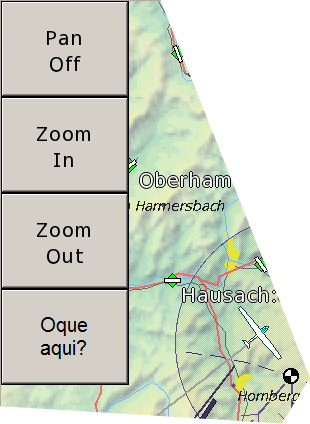
\includegraphics[angle=0,width=0.75\linewidth,keepaspectratio='true']{figures/pan.png}
\end{center}\index{Was ist hier?}
Mit der Auswahl von \button{Was ist hier} öffnet sich ein Menü, welches entsprechende Kartenelemente wie z.B.\ Wegpunkte und Lufträume die sich in der Nähe des Fadenkreuzes befinden, sowie die eigene Position anzeigt und zur Auswahl/Bearbeitung darstellt. Zu den jeweiligen angezeigten Elementen werden Entfernung und ggf.\ benötigte Höhe angezeigt.

Parallel dazu werden in der oberen rechten Bildschirmecke die Koordinaten des Fadenkreuzes und die dazugehörige Höhe des Geländes über MSL angegeben.  

%%%%%%%%%%%%%%%%%%%%%%%%%%%%%%%%%%%
\section{Wegpunkte} \label{sec:waypoint-schemes}
Die Darstellung und Einfärbung von Wegpunkten erfolgt je nach Situation und Art des jeweiligen Punktes.\menulabel{\bmenut{Konf}{2/3}\blink\bmenus{System}} Hauptmerkmal ist die hierbei Landbarkeit bzw. Erreichbarkeit eines Wegpunktes.

Es gibt derzeit drei verschiedene Icon- Sätze  für die Darstellung von landbaren Wegpunkten  (Lila Punkt, Schwarz Weiß und Ampel), die unter \index{Wegpunkte!Farben}
\button{Landbare Symbole} ausgewählt werden können.\menulabel{\button{Kartenanzeige}\blink\button{Wegpunkt}}\index{Wegpunkte!Darstellung}

\begin{description}
   \item[\p{Lila Punkt}] Bei dieser Darstellung werden die landbaren Plätze als lila Punkt angezeigt. Wenn der Wegpunkt erreichbar ist, bekommt der lila Punkt einen grünen Kreis.  Diese Darstellung ist sehr ähnlich der in WinPilot
   \item[\p{S/W}] \config{waypointicons} Landbare Wegpunkte werden in der Karte weiß/grau dargestellt, ähnlich wie oben bekommen erreichbare Plätze einen grünen Punkt, ist er durch einen Berg versperrt, wird er rot. 
   \item[\p{Verkehrsampel}] Flugplätze und Außenlandefelder werden in den Farben einer Verkehrsampel dargestellt: Grün, wenn erreichbar, Orange, wenn z.B.\ durch einen Berg versperrt und rot, wenn er überhaupt nicht erreicht werden kann.
\end{description}

\tip Je nach verwendeter Datenbank kann auch die Länge und Richtung der Landebahn mit angezeigt werden. 
Weiterhin können je nach Sichtbarkeit bzw. Erreichbarkeit die Farben und/oder Formen geändert werden.

Die Symbole sind in untenstehender Tabelle aufgelistet. 

\begin{tabular}{c|c|cc|ccc|} 
\textbf{Darstellung:} &\begin{sideways}Einfacher Wegpunkt \end{sideways}
&\begin{sideways}WP landbar,  n.  erreichbar\end{sideways}
&\begin{sideways}WP erreichbar\end{sideways}
&\begin{sideways}Flugplatz n. erreichbar\end{sideways}
&\begin{sideways}Flugplatz erreichbar\end{sideways}
&\begin{sideways}Flugplatz versperrt\end{sideways}\\
\hline
''Lila Kreis'' &
\includegraphics[width=0.5cm]{icons/map_turnpoint.pdf} &
\includegraphics[width=0.85cm]{icons/winpilot_landable.pdf} &
\includegraphics[width=0.85cm]{icons/winpilot_reachable.pdf} &
\rule[0em]{0em}{2.5em}\colorbox{white}{\includegraphics[width=0.85cm]{icons/winpilot_landable.pdf}}
& \includegraphics[width=0.85cm]{icons/winpilot_reachable.pdf} 
& \includegraphics[width=0.85cm]{icons/winpilot_marginal.pdf} \\
\hline
''Schwarz/Weiß''  &
\includegraphics[width=0.5cm]{icons/map_turnpoint.pdf} &
\includegraphics[width=0.75cm]{icons/alt_landable_field.pdf} &
\includegraphics[width=0.75cm]{icons/alt_reachable_field.pdf} &
\rule[0em]{0em}{2.5em}\colorbox[rgb]{0.94,0.94,0.94}{\includegraphics[width=0.75cm]{icons/alt_landable_airport.pdf}}
& \includegraphics[width=0.75cm]{icons/alt_reachable_airport.pdf} 
& \includegraphics[width=0.75cm]{icons/alt2_landable_field.pdf}\\
\hline
''Verkehrsampel'' &
\includegraphics[width=0.5cm]{icons/map_turnpoint.pdf} &
\includegraphics[width=0.75cm]{icons/alt2_landable_field.pdf} &
\includegraphics[width=0.75cm]{icons/alt_reachable_field.pdf} &
\rule[0em]{0em}{2.5em}\colorbox{white}{\includegraphics[width=0.75cm]{icons/alt2_landable_airport.pdf}}
&\includegraphics[width=0.75cm]{icons/alt_reachable_airport.pdf} 
&\includegraphics[width=0.75cm]{icons/alt2_marginal_airport.pdf}\\
\hline
\end{tabular}
%
 
Die Wegpunkte können nach mehreren Abkürzungsregeln beschriftet werden, um auf \config{labels}
\menulabel{\bmenut{Anzeige}{2/3}\blink\bmenut{Beschriftung}{Aufgabe}} der Karte nicht so viel Platz zu verschwenden und den Bildschirm  übersichtlicher darstellen zu können. 
So können die Beschriftung der Wegpunkte nur für die Aufgabe, für Aufgabe und Landeplätze oder aber für alle Wegpunkte aktiviert weren.


\xc berechnet kontinierlich und unter Berücksichtigung des Windes, welche Wegpunkte sich innerhalb des Gleitpfades befinden und stellt dies entsprechend der eingestellten Optionen dar.

Die angenommene Ankunftshöhe {\em oberhalb der Sicherheitshöhe} der erreichbaren  Wegpunkte wird neben dem Wegpunkt  angezeigt. Diese Ankunftshöhe wird berechnet aus der entsprechenden Leistung des Segelflugzeuges und dem MacCready Wert. 

\config{reachpolar} Hierbei kann gewählt werden, ob die Berechnung mit einem Sicherheits-MacCready Wert, oder aber streng nach der Polare erfolgt.

\subsection*{Nicht landbare Wegpunkte}
Wenn in der  Wegpunktdatenbank bzw. in der Beschreibung des einzelnen Wegpunktes informatiuonen zu dessen beschaffen heit angegeben sind, so werden diese von \xc   entsprechend dargestellt. In der folgenden Tabelle  sind die nicht landbaren Wegpunkte aufgelistet. 

\vspace{9em}
\begin{center}
\begin{small}
\begin{tabular}{ccccccccc}
\begin{rotate}{60}Einfacher Wegpunkt\end{rotate} &
\begin{rotate}{60}Berggipfel\end{rotate} &
\begin{rotate}{60}Aussicht\end{rotate} &
\begin{rotate}{60}Berg-Pass\end{rotate} &
\begin{rotate}{60}Kraftwerk\end{rotate} &
\begin{rotate}{60}Turm/hohes Gebäude\end{rotate} &
\begin{rotate}{60}Tunnel\end{rotate} &
\begin{rotate}{60}Wetterstation\end{rotate} &
\begin{rotate}{60}Brücke\end{rotate}\\
\includegraphics[width=0.5cm]{icons/map_turnpoint.pdf} &
\includegraphics[width=0.8cm]{icons/map_mountain_top.pdf} &
\includegraphics[width=0.7cm]{icons/map_obstacle.pdf} &
\includegraphics[width=0.7cm]{icons/map_pass.pdf} &
\includegraphics[width=0.8cm]{icons/map_power_plant.pdf} &
\includegraphics[width=0.7cm]{icons/map_tower.pdf} &
\includegraphics[width=0.6cm]{icons/map_tunnel.pdf} &
\includegraphics[width=0.6cm]{icons/map_weather_station.pdf} &
\includegraphics[width=0.8cm]{icons/map_bridge.pdf} \\
\end{tabular}
\end{small}
\end{center}


%%%%%%%%%%%%%%%%%%%%%%%%%%%%%%5
\section{Aktive Aufgabe}

Die Kurslinie der aktiven Aufgabe wird als eine grüne, gestrichelte Linie auf der Karte dargestellt.

Bei AAT-Aufgaben werden die Sektoren der Aufgabe gelb transparent hinterlegt dargestellt.
Die Start und Zielpunkte werden als Kreise dargestellt, Linien werden nur 
gezeichnet, wenn es sich hierbei um Start bzw. Ziellinien handelt.
Wendepunktsektoren werden als Segmente dargestellt (auch der DAEC-Schlüssellochsektor kann dargestellt werden).


Vom Segelflugzeugsymbol wird eine dicke schwarze Linie direkt zum nächsten aktiven Wendepunkt gezeichnet. Diese Linie stellt normalerweise den direkten Weg zum nächsten Wegpunkt dar, kann aber auch eine {\em Route} darstellen, welche um zum Beispiel Berge und/oder Lufträume herum führt. Nähere Details hierzu werden im Abschnitt Route~\ref{sec:route}  beschrieben.
\begin{center}
\begin{tabular}{c c c}
{\it Start/Ziel} & {\it Sektor} & {\it Zylinder} \\
\includegraphics[angle=0,width=0.3\linewidth,keepaspectratio='true']{figures/cut-startfinish.png} &
\includegraphics[angle=0,width=0.3\linewidth,keepaspectratio='true']{figures/cut-sector.png} &
\includegraphics[angle=0,width=0.3\linewidth,keepaspectratio='true']{figures/cut-barrel.png} \\
\end{tabular}
\end{center}
%%%%%%%%%%%%%%%%%%%%%%%%%55
\section{Gelände und Topologie}

Die folgenden topologischen Details werden auf der Karte dargestellt:
\begin{itemize}
\item Hauptstraße, dargestellt als rote Linien
\item Flüsse, dargestellt als blaue Linien
\item Große Wasserflächen (Seen), dargestellt als blaue Flächen
\item Große Städte, dargestellt als gelbe Flächen
\item Kleine Siedlungen, dargestellt als gelbe Diamanten, je nach verwendeter Datenbank wird auch nur der Name angezeigt 
\end{itemize}
Großstädte und kleine Siedlungen werden in Schrägschrift beschriftet.

Das Gelände wird gemäß der Höhe eingefärbt, optional kann es schattiert werden -  entweder gemäß der Sonneneinstrahlung oder aber entsprechend des Windeinfalles (Luv oder Lee).

Unbekanntes Gelände, oder Gelände das unterhalb der Meereshöhe liegt, wird blau dargestellt.

Die Schattierung des Geländes erhöht die Erkennbarkeit der Struktur und ist derzeit so gestaltet, daß helle Flächen eines Berges die Luvseite darstellen \config{shading}. und dunkle Flächen die Leeseite.
Die Stärke und Helligkeit der Schattierung kann konfiguriert werden 

Die Unterstützung der Schattierung für Sonneneinstrahlung in Abhängigkeit vom \menulabel{\bmenut{Anzeige}{2/2}\blink\bmenut{Gelände}{An}}Sonnenstand ist in Arbeit\dots.
Gelände- und Topologiedarstellung kann über das Menü ein und ausgeschaltet werden:

\menulabel{\bmenut{Anzeige}{2/2}\blink\bmenut{Topologie}{An}}
\begin{center}
\begin{tabular}{c c}
Topology & Terrain \\
\includegraphics[angle=0,width=0.4\linewidth,keepaspectratio='true']{figures/cut-topo.png} &
\includegraphics[angle=0,width=0.4\linewidth,keepaspectratio='true']{figures/cut-terrain.png} \\
\end{tabular}
\end{center}

Wenn keine Geländedaten zur Verfügung stehen (oder die Gelände-Anzeige ist abgeschaltet) erscheint der Hintergrund der Karte weiß. Jedes Gelände unterhalb des Meeresspiegels wird blau dargestellt!
Flüge außerhalb des in der Datenbank bekannten Geländes werden weiß dargestellt.

\menulabel{\bmenut{Anzeige}{2/2}\blink\bmenut{Beschriftung}{Alle}}
Um die Darstellung auf der Karte übersichtlicher zu machen, können Beschriftungen und Labels der Wegpunkte ein und ausgeschaltet werden, oder aber auf die aktive Aufgabe beschränkt werden.

Folgende Auswahlen stehen zur Verfügung:

\jindent{\bmenud{Beschriftungen}{Aufgabe \&}{ Landeplätze}}{ Zeigt die Beschriftung der Wegpunkte  der aktiven Aufgabe und einige landbare Felder (basierend auf den Wegpunkt-Details in der geladenen Wegpunkt Datei).  Andere Wegpunkte werden angezeigt, aber nicht beschriftet. }
\jindent{\bmenut{Beschriftung}{Aufgabe}}{ Es werden nur die in der aktiven Aufgabe befindlichen Wegpunkte beschriftet. }
\jindent{\bmenut{Beschriftung}{Alle}}{ Anzeige aller Beschriftungen für alle Wegpunkte. }

Die Beschriftung und das Aussehen der Beschriftung ist über das Menü \config{labels} konfigurierbar.
%%%%%%%%%%%%%%%%%%%%%%55
\section{Flugspur (trail)}\label{sec:trail}

Wenn gewünscht, kann die bisher geflogen Flugstrecke auf der Karte dargestellt werden. Die Farbe und die Breite dieser Spur hängt von der Höhe oder von Vario-Wert ab und kann entsprechend gewählt werden. \config{snailtype}

\begin{center}
\includegraphics[angle=0,width=0.75\linewidth,keepaspectratio='true']{figures/snail.pdf}
\end{center}

Wenn ein VEGA-Variometer angeschlossen ist und die Netto-Luftmassenbewegung anzeigt, dann können die Farben und Dicken dieser Spur auch die Netto-Luftmassenbewegung darstellen.

Die Flugspur kann wie folgt ausgewählt werden: \button{Kurz} (zeigt ungefähr 10 min), \menulabel{\bmenut{Anzeige}{2/2}\blink\bmenut{Spur}{Kurz}} \button{Lang}, (zeigt ca. eine Stunde), \button{Voll} (zeigt die gesamte bisherige Flugstrecke) und aus. Die Einstellung kann jederzeit über das Menü wie folgt vorgenommen werden:

Alternativ kann die Einstellung auch im Menü  \config{snailtrail} als Voreinstellung eingestellt werden.
Beachtet, daß wegen der Übersichtlichkeit der Kartendarstellung beim Kurbeln die Flugspur grundsätzlich kurz ist.
%%%%%%%%%%%%%%%%%%%%%%%%%%%%%%
\subsection*{Spurdrift (Windversatz-Kompensation)}
Um den Windversatz beim Kurbeln darzustellen und so das Zentrieren zu unterstützen, kann die Spurdrift-Funktion bei der Kartendarstellung eingeschaltet werden.

 \textcolor{blue}{ Die Spurdrift bzw. Windversatz-Kompensation nach Kap.\ref{sec:Windeinstellung} hat \textbf{nichts}  mit der Funktion ''geschätzte Windabdrift'' \achtung aus der Endanflugskonfiguration nach Kap.~\ref{sec:final-glide} zu tun!}
 
In diesem Fall wird die Flugspur relativ zum Wind aufgezeichnet und nicht mehr absolut über Grund. Das bedeutet, daß  \xc den erflogenen Bart während des Fluges mit dem ermittelten Wind versetzt ganz ähnlich wie auch das Flugzeug versetzt wird. Hiermit wird eine bessere Wiederauffindbarkeit und  Anzeige der Bewegung des Flugzeuges relativ zum Bart ermöglicht.

Zur Veranschaulichung ist nachfolgend ein Beispiel beigefügt. 

Beachte, daß, wenn die Spurdriftfunktion aktiviert ist (rechtes Bild), sich das Flugzeug mehr in einem parallelversetzten Kreis  bewegt, anstelle einer gekrümmten, langgezogenen Spirale (linkes Bild).

\begin{center}
\includegraphics[angle=0,width=0.8\linewidth,keepaspectratio='true']{figures/traildrift.png}
\end{center}

\config{traildrift} Die Funktion \button{Spurdrift} kann über die Konfiguration Einstellung ein und ausgeschaltet werden.  Die Kompensation ist ausschließlich in Kurbelmodus aktiv; im normalen Geradeausflug wird eine Kompensation über das Wind-Menü ermöglicht.
\menulabel{\bmenus{Konfig}\blink\bmenus{Wind}}
Die Anzeige des Windversatzes zeigt sehr schön, wenn Bärte in der Höhe stark versetzt werden - zum Beispiel durch Windscherungen.

Die Breite der Flugspur  kann optional anhand des Vario-Wertes gesetzt werden (Steigen, Saufen) \config{trailscaled}.
%%%%%%%%%%%%%%%%%%%%%%%5
\section{Marker}

Marker werden als kleine blaue Flaggen auf der Karte dargestellt. 
Die Marker können entweder automatisch oder aber durch Knopfdruck gesetzt werden.

\menulabel{\bmenut{Nav}{2/2}\blink\bmenut{Marke}{Setzen}}Ein Beispiel für die Nutzung von automatischem Setzen von Markern ist z.B. die 
Markierung, wann in den Kurbelmodus gewechselt wurde. Hiermit kann sehr einfach dargestellt werden, wann und wo gekurbelt wurde.\index{Marker}
\menulabel{\includegraphics[angle=0,width=0.5cm,keepaspectratio='true']{icons/map_flag.pdf}}

Marker werden nicht gespeichert, wenn \xc beendet wird, die Koordinaten aller Marker werden jedoch im File \verb|xcsoar-marks.txt| gespeichert.

%%%%%%%%%%%%%%%%%%%%%%%%%%%%%%
\section{Anzeige des Gleitbereiches}\label{sec:reach}

Der aktuelle Gleitbereich \button{Erreichbar Anzeige}kann wahlweise in der Karte auf zwei Weisen dargestellt werden:\index{Gleitbereich}\index{Gleitbereich!Darstellung}\index{Reichweite}
\menulabel{\bmenut{Konfig.}{2/3}\blink\bmenus{System}}
\begin{itemize}
    \item als schwarz-weiß gestrichelte Linie, 
    \item als schattierter Bereich.
\end{itemize}
\menulabel{\button{Endanflug}\blink\button{Routenplaner}}
Der Gleitbereich schließt alle erreichbaren Gelände ein und markiert - entsprechend der Höhe des Geländes - auch Bereiche, welche evtl.\ umflogen werden müssen.  Dies kann sehr nützlich sein, wenn in niedrigen Höhen nach Steigen gesucht wird, oder man sich in bergigem Gelände aufhält.

Die Berechnung der Reichweite \button{Reichweite Modus} kann in zwei Detailstufen \config{turningreach} wie folgt konfiguriert werden:

\begin{description}
\item[\p{Aus}] Wenn ausgeschaltet, wird die Reichweite nicht berechnet.
\begin{center}
\includegraphics[angle=0,width=0.8\linewidth,keepaspectratio='true']{figures/reach2.png}
\end{center}
\item[\p{Direkt}] Wenn eingeschaltet, erfolgt die Berechnung der Reichweite geradeaus vom Flugzeug. Es werden weder Lufträume noch sonstige Hindernisse in die Kalkulation einbezogen.\index{Gleitbereich!Berechnung}
 \item[\p{mit Umweg}] Wenn dies eingeschaltet ist, wird die Reichweite unter Berücksichtigung von max.\ drei 90$^\circ$ Kurven errechnet, die z.B.\ zum umfliegen von kleineren Hindernissen bzw.\ zum Umschauen benötigt werden. Diese Reichweite ist entsprechend geringer (s.\ Bilder)
\begin{center}
\includegraphics[angle=0,width=0.8\linewidth,keepaspectratio='true']{figures/reach1.png}
\end{center}
\end{description}

Der Weg des Endanfluges wird permanent auf evtl.\ Kollisionen mit einer Geländeerhebung geprüft -- sollte sich eine Kollisionsgefahr ergeben, so wird der vorausgesagte Kollisionspunkt\index{Geländekollision} mit dem Gelände als kleines rotes Kreuz auf der Karte dargestellt.

Wenn der \button{Reichweite Modus} aktiviert ist, dann wird dieser bei Abbruch einer Aufgabe  automatisch benutzt, um landbare Plätze (in allen Richtungen) auf der Karte darzustellen (Im Alternativen - Modus).


\textcolor{blue}{Beachte, daß bei aktiven Aufgaben die ''Reichweite'' Funktion   \textbf{nicht} in den InfoBoxen aktiv ist, hier wird die Funktion \textbf{nicht} verwendet!}\warning 


\textcolor{blue}{Sie ist ausschließlich bei der Darstellung auf der Karte und bei abgebrochenen Aufgaben aktiv!}

Die Leistungsdaten des Segelflugzeuges (Polare) bzw.\ die MacCready Einstellung, die für diese Berechnung verwendet werden sollen, können unter %\ref{sec:final-route}
\button{Erreichbare Polare} eingestellt werden. \config{reachpolar}
\begin{description}
\item[\p{Aufgabe}] Es wird der MC benutzt, welcher in der Aufgabe gesetzt ist.
\item[\p{Sicherheits  MC}] Hier wird ein voreingestellter, i.d.R.\ niedriger MC Wert gewählt, den der Pilot vorher festsetzt. Normalerweise etwas schlechter als das beste Gleiten. (s.~\ref{safety-MC}) 

Die ''Größe'' der Sicherheit bei der Reichweitenkalkulation ist dementsprechend   die Differenz aus bestem Gleiten und dem Gleiten entsprechend der Geschwindigkeit des Sicherheits MC-Wertes.
\end{description}
%%%%%%%%%%%%%%%%%%%%%%%%%%%%%%%%%%%%%%%%%5
\section{Status-Fenster}\label{sec:aircr-stat-dial}\index{Status}

Das Status-Fenster ist ein reines Informationsfenster und hat fünf Unterfenster. \button{Flug}, \button{System}, \button{Aufgabe}, \button{Regeln} und \button{Zeiten} Es 
\menulabel{\bmenut{Info}{2/3}\blink\bmenus{Status}} und dient vor allem zur Beobachtung von Zeiten, Koordinaten, Regeln etc.\  
  
\achtung Beachte, daß die hier aufgeführten Daten \textbf{nicht} aktualisiert werden, während dies Fenster geöffnet ist. erst nach Schließen und wieder aufrufen sind die Daten wieder auf dem laufenden! 

Mit dem Button \button{Flug} kann z.B. schnell Deine Position an andere 
weitergegeben werden, hier wird Deine Position angezeigt, Deine Peilung und Entfernung auf den nächsten aktiven Wegpunkt etc. 


Derzeit werden als ''nächste Wegpunkte'' ausschließlich Punkte aus der Wegpunkt-Datenbank genommen, in zukünftigen Versionen ist geplant, evtl.\  auch Dörfer und Städte aufzunehmen.%\menulabel{\includegraphics[angle=0,width=0.8\linewidth,keepaspectratio='true']{figures/status-flight.png}}
\sketch{figures/status-flight.png}

Unter \button{Regeln}kannst Du z.B.\ erkennen, ob Dein Abflug gültig war, mit welcher Geschwindigkeit er erfolgte etc.\ 

\button{Zeiten}gibt allerlei Zeiten wieder, z.B.\ die UTC-Zeit, den Sonnenauf- und Untergang (Danke, Helmut\dots), Start- Lande- und Flugzeit. 

\button{System}informiert u.a.\ über die Versorgungsspannung des Geräte, wie der GPS-Empfang ist, ob \fl und Logger angeschlossen sind. 

In \button{Aufgabe}werden Daten und Zeiten zur aktuellen Aufgabe gelistet: aktueller Schnitt, Distanz, bei AAT: zugeteilte und verbleibende Zeit etc\dots 


%%%%%%%%%%%%%%%%%%5
\section{Routen}\label{sec:route}

\xc kann Flugwege planen, die um Lufträume und z.B.\ Gebirge herumführen, sowohl in \menulabel{\bmenut{Konfig.}{2/3}\blink\,\bmenus{System}}
horizontaler als auch in vertikaler Richtung. Solch ein Flugweg wird hier als ''Route'' bezeichnet und kann mit dem \button{Routenplaner} konfiguriert werden..

\menulabel{\qquad\button{Endanflugrechner}} 
Die Höhe des Zieles ist hierbei die Ankunftshöhe des Zieles, kann aber auch größer sein, falls die Wegführung durch die in der Aufgabe deklarierten Wegpunkte dies erfordern. Die Routen-Funktion ist in folgenden Flugmodi verfügbar:

''Gehezu'', deklarierte (aktive) ''Aufgaben'' und ''Abbruch''.

\begin{center}
\includegraphics[angle=0,width=0.75\linewidth,keepaspectratio='true']{figures/route3.png}
\end{center}

Im obigen Bild kannst Du gut erkennen, wie die ''Route'' einen Knick nördlich des Harzes macht, um nicht ins Gelände zu ''stürzen'', der normale Kurs ist gestrichelt weiter südlich zu sehen. 

Bei der Routenberechnung wird die Strecke unter Berücksichtgung der Flugzeugpolaren zeitoptimiert berechnet. Standardmäßig ist die Routenfunktion ausgeschaltet. Sie kann aktiviert werden unter  \config{routemode} Berücksichtigung von Lufträumen, Gelände, Wolkenuntergrenze.

Geländekollisionen in vertikaler Richtung werden verhindert durch Einstellung der Gelände-Sicherheitshöhe. \config{safetyterrain} Hierbei ist keine zusätzliche Höhe als Puffer vorgesehen.

Es kann sein, daß manche Routen in einer Ankunft am Ziel höher als erwartet enden. Dies kann zum Beispiel geschehen, wenn der Zielpunkt exakt hinter einem relativ hohen Berg liegt. Zur Vermeidung von horizontalem Einfliegen in einen Luftraum wird mit ein Sicherheitsabstand von 250 m ohne weitere vertikaler Reserven benutzt.
Richtig deklarierte Routen werden im Flugverlauf über oder unterhalb Lufträumen und auf jeden Fall um Lufträume herum führen.

\warning
Wenn der MacCready-Wert größer als 0, dann ist für den Rechner das Steigen während einer Route gemäß der MC-Theorie ''erlaubt''. \config{routeceiling}  Die maximale Höhe des Steigens  ist auf  500 m unterhalb der Wolkenuntergrenze limitiert, kann jedoch in der Konfiguration abgeschaltet werden.

Ein Steigen über die maximal vorgeschriebene Höhe des Start- und Zielpunktes (siehe oben) wird ''bestraft'' mit einer entsprechend schlechteren Steigrate als der aktuell eingestellte MacCready-Wert. 


Einige Einschränkungen und Limitierung bezüglich des Routenplanungssystems sind hier aufgelistet:

\begin{itemize}
\item Wenn Kurbeln notwendig ist, um das Ziel zu erreichen,  wird angenommen, daß das Steigen zu Beginn der Route ist. 

Hintergrund: eine Einstellung von  MacCready gleich 0 bedeutet, daß (streng nach der MC-Theorie) kein Steigen erwartet wird!  Andernfalls würde die Rechenalgorythmen in  die Irre geführt werden!   
\item Strecken mit Steigen im Geradeausflug werden auf einer konstanten Höhe angenommen, gleichbedeutend mit vielen kleinen Steigen verteilt entlang der Strecke
\item Kurven und Schlenker zwischen den einzelnen Streckensegmenten mit Ablagen größer 90$^\circ$ sind erlaubt
\item Fehler des Rechenalgorithmus innerhalb der Route können dazu führen, daß der Anflug in einem direkten Anflug auf das Ziel zurückgeführt wird.
\end{itemize}


\subsection*{Querschnitt des Geländes und Lufträume auf Kurs (''cross-section'', ''xs'')}
\label{cross-section}\index{Gelände- und Luftraumquerschnitt auf Kurs}\index{Cross-Section (XS)}

Seit Version 6.5 kann auf Wunsch  ein Querschnitt der Fin lugrichtung liegenden
\menulabel{\bmenut{2/3}{Konf.}\blink\bmenus{System}} Lufträume sowie des Geländes
dargestellt werden. Hier sind im oberen Bereich alle derzeit verfügbaren InfoBox-Seiten
aufgelistet und es kann aus gewählt werden, was explizit in welchem Bereich des Bildschirmes
 \menulabel{\bmenus{Aussehen}\blink\bmenus{Seiten}} dargestellt werden soll.
 Darunter ist ein Auswahlbereich vorgesehen, in dem folgende
Möglichkeiten zur Auswahl stehen:
 \begin{description}
 \item[\p{Zentral}] Karte, \fl-Radar, Zentrierhilfe
 \item[\p{InfoBoxen}] Alle derzeit vorhandenen InfoBox-Seiten (max. acht Stück !) werden hier
     zur Auswahl dargestellt. Aux 1 .. Aux 8, Endanflug, Auto, beim Kreisen etc\dots
 \item[\p{Unten}] Nichts, Querschnitt
 \end{description}

Mit der Auswahl \button{Zentral}-- \button{\fl-Radar}kann z.b. eine Seite definiert werden,
auf der als zentrales Element das \fl-Radar dargestellt wird, klickt man dazu unter
\button{Unten} den Punkt \button{Querschnitt}an, wird auf dieser Seite im unteren Bereich der
Querschnitt des auf Kurs liegenden Geländes und der Lufträume mit einem entsprechenden
Maßstab und der Höhe, links am Rand als kleiner schwarzer Pfeil dargestellt. Diese
Querschnitts-Darstellung  wird permanent aktualisiert und stellt so einen schönen  vertikalen
Überblick über das voraus liegende Gelände in Verbindung mit den zu erwartenden Lufträumen
dar.

\begin{center}
\hspace{7.5em}\includegraphics[angle=0,width=0.75\linewidth,keepaspectratio='true']{figures/map-cross-section.png}
\end{center}

Die Querschnitt-Darstellung ist  derzeit nicht skalierbar sondern hat einen fixen horizontalen
Maßstab von 45km und ist auf eine Höhe von 3000m begrenzt.

%Auf diese Art und Weise kann man sich beliebige Infobox-Seiten mit Zusatzinformationen
%erstellen, in welchem z.B.\  beim engen Kurbeln nahe an Lufträumen sehr schön die
%Zentrierhilfe als zentralem Bestandteile der Anzeige und im unteren Bereich der Querschnitt
%über das Gelände dargestellt wird. Diese Seite kann dann als z.B.\ "Kurbeln" bezeichnet und
%abgespeichert werden.

% eben leider nicht  ...  wenn Zentrierhilfe eingeschaltet ist, erscheint cross section nicht.
% bug oder feature ??

Mit den Hoch- und Runterpfeilen kann die Priorität bzw.\ Reihenfolge des Aufrufes der Seiten
auf dem Bildschirm bestimmt werden.  Es ist somit jedem selbst überlassen, wie er sich diese
Anzeigen zurechtlegt.

Mit \button{Hinzufügen} kann eine neue InfoBoxSeite hinzugefügt werden, bis die maximale
Anzahl von 8 Stück erreicht ist.

Mit dem Pfeil nach rechts gelangt man sofort in das InfoBox-Seiten Menü, auf welchem die
einzelnen InfoBoxen innerhalb der Seite definiert und angeordnet  werden können.Die

 \subsection*{\textcolor{blue}{\textbf{{\large Einschränkungen der
Querschnittsdarstellung:}}}}

Die Querschnittfunktion funktioniert derzeit \textbf{nicht} in Verbindung mit der Zentrierhilfe als zentralem Kartenausschnitt!

Die Querschnittfunktion funktioniert derzeit \textbf{nicht} in Verbindung mit dem \fl-Radar als zentralem 
Kartenausschnitt!

\warning {\textbf{Aufgrund technischer
Probleme mit den diversen Betriebsystemen (insbesondere Windows und PPC / Mobile) ist es
derzeit nicht möglich, die Gesten \emph{innerhalb} dieser Area des Bildschirmes beginnen bzw.
Enden zu lassen.}} 

Wenn mit Gesten gearbeitet werden soll, müssen diese daher außerhalb des
Anzeigebereiches des Querschnittes beginnen und enden!

Dies kann zu ungewohnter Arbeitsweise im Fluge führen, da ansonsten die Gesten nicht
ordnungsgemäß ausgeführt werden! Besonders betroffen sind davon Gesten, welche unten
beginnen - diese müssen dann ein Stück weiter oben begonnen werden !!



%%%%%%%%%%%%%%%%%%%%%%
\setcounter{chapter}{4}
\chapter{Überlandflug Aufgaben - Navigieren mit\textsf{XCSoar}}\label{cha:tasks}
\index{Aufgabe}\index{Tasks}

\textsf{XCSoar} bietet ein ausgefeiltes, komplettes Aufgabenmanagementsystem, mit dem Aufgaben vor und während des Fluges erstellt, editiert und auch gelöscht werden können.

Die Wendepunkte können vollautomatisch angeflogen und umgestellt werden, wobei die Kartendarstellung automatisch hinein- bzw. herausgezoomt werden kann. Ein rein manuelles  Anwählen und Umschalten ist aber ebenso möglich.

Dieses Kapitel beschreibt weiterhin die Benutzung von \textsf{IGC} Loggern mit\textsf{XCSoar}

Intern werden drei Aufgabentypen (modi)  unterschieden
\begin{description}
\item[\p{Deklarierte Aufgabe}] Dies ist der eigentliche Überlandflug-Modus, bei dem ein Startpunkt, ein
    Zielpunkt und mehrere Wendepunkte deklariert sein können. Die Wendepunkte müssen in der
    angegeben Reihenfolge angeflogen werden. (Leistungsflug)\index{Task!Leistungsflug}
\item[\p{''Ziele auf''-- Aufgabe}] Ein Flug auf exakt ein einziges Ziel zu. (Irgendein Flug)\index{Task!Zielflug}
\item[\p{Abort - Aufgabe}] Hier wird "frei" durch die Gegend geflogen, ohne einen Wegpunkt als  Ziel
    deklariert zu haben. (Lustflug)\index{Task!Lustflug}
\end{description}

 Beachte, daß im ''Ziele auf''- und im Abort - Modus  die  evtl.\ abgebrochene Aufgabe \textsl{jederzeit} wieder \tip aufgenommen werden kann, dies unter Beibehaltung sämtlicher bisher aufgenommenen Berechnungen und Statistiken.

\section{''Ziele auf''-- Aufgabe}\index{Aufgabe!''Ziele auf'-'-Typ}\index{Task!''Ziele auf''}

''Ziele auf''--Aufgaben'' können erstellt werden, indem man einen Wegpunkt auf der Karte markiert und anschließend auf dem ''Kartenelemente an diesem Ort'' oder dem Wegpunkt-Detailfenster mit "Ziele auf" bestätigt.  Alternativ kann auch über den "Alternative" Dialog zu einem Wegpunkt gelangt werden, welcher anschließend mit ''Ziele auf'' festgelegt wird.

Während des ''Ziele auf''--Modus \menulabel{\bmenut{Nav}{2/2}\blink\bmenut{Aufgabe}{fortsetzen}} kann eine vorher abgebrochene Aufgabe immer wie links fortgesetzt werden.

\subsection{Automatik ''Ziele auf''}\index{Automatik--''Ziele auf''}\index{Heimatflugplatz!Automatik}

Wenn keine deklarierte Aufgabe geladen ist, dann wird nach dem Start unverzüglich in den ''Ziele auf''--Modus geschaltet. Hierbei wird der Startplatz oder aber (falls es z.B. eine Wiese war, von der man mit einer Wilga im F-Schlepp gestartet ist), der nächstgelegene landbare Flugplatz automatisch als Ziel in den Rechner eingefügt.

Egal, ob eine Aufgabe deklariert wurde, oder nicht, es wird grundsätzlich ein Startpunkt erfaßt, welcher für spätere Benutzung während des Fluges in der Wegpunktliste erscheint und ganz normal  verwendet werden kann. 
Dieser Punkt ist auf der Karte als ''take-off' gekennzeichnet' \todonum{wird der auch gespeichert? wo ?}

\section{Aufgaben erstellen und bearbeiten}\index{Aufgabe!Erstellen}\index{Aufgabe!Bearbeiten}

Aufgaben können auf unterschiedliche Weise erstellt und editiert  werden. Manche Methoden eigentlich mehr für die Bearbeitung und Erstellung vor dem Flug,  andere erlauben es eine Aufgabe während des Fluges zu ergänzen bzw. zu verändern.

Aufgaben können in Dateien (Files) gespeichert werden um später geladen zu werden oder aber um zwischen verschiedenen Geräten hin und her kopiert zu werden. Alle\textsf{XCSoar} Plattformen sind Dateiformatskompatibel d.h.\  jede Aufgabe kann auf jedem\textsf{XCSoar} erstellt, geflogen und gespeichert werden. (\textsf{PC, Android, MAC)}).

\tip Es ist möglich (und sinnvoll) eine Standard-Aufgabe zu erstellen und zu speichern und diese  Aufgabe beim jedem Start von\textsf{XCSoar} automatisch laden zu lassen.

Eine Anwendung dieser Standardaufgabe ist zum Beispiel, einen Wegpunkt  als Heimatflughafen zu deklarieren. d.h.,  der Heimatflugplatz ist anschließend grundsätzlich automatisch als Ziel eingestellt, wenn man einfach nur durch die Gegend fliegen will.

Die Möglichkeiten, Aufgaben zu erstellen sind wie folgt:
\begin{itemize}
\item Benutzen des Aufgabeneditor-Dialogs
\item Auswählen eines Wegpunktes von der Karte und hinzufügen zur Aufgabe über den Wegpunkt Detail-Dialog.
\item Laden einer Aufgabe aus einer Datei.
\end{itemize}

\tip Aufgaben in einer Datei zu sichern und anschließend wieder zu laden ist sehr sinnvoll,  will man zum Beispiel mit mehreren Piloten eine gleiche Aufgabe fliegen oder aber im Wettbewerb ist, wo im  allgemein die Aufgaben vorher deklariert und eingegeben werden.

Entscheidend hierbei ist, daß lediglich eine Person die Aufgabe eingeben muß und diese anschließend  per copy \& paste,  Bluetooth oder Kabel kopiert werden kann.

\textsf{XCSoar} sichert die aktuelle Aufgabe beim Herunterfahren und lädt die gleiche Aufgabe wieder beim Neustart.  Die Wegpunkte einer Aufgabe sind sogar gesichert, wenn die Wegpunktdatei gewechselt wird. d.h., wenn eine Aufgabe gespeichert wird, anschließend das Wegpunktfile gewechselt wird, die gleiche Aufgabe wieder geladen  wird, wenn die Wegpunkte, welche in der Wegpunktdatei  fehlen automatisch durch die Wegpunkte aus der Aufgabe ergänzt.

\section{Wegpunkt Info und Details }\index{Wegpunkte!Details}

Der Wegpunkt-Info-Dialog beschreibt die Details der Wegpunkte  und bietet Navigations-Optionen wie zum Beispiel \textsf{Ziele auf}, \textsf{Einfügen} oder \textsf{Anhängen} an einer Aufgabe. Weiterhin kann über diesen Dialog ein Wegpunkt als Heimatflughafen eingegeben werden.

Die Anwahl  kann über mehrere Wege erfolgen:
\begin{itemize}\itemsep=1em
\item
Über die Karte, wenn der Wegpunkt sichtbar ist: \\
Ein \textit{einfacher} Klick öffnet das "Kartenelemente an diesem Ort''-Fenster.

Anschließend auf \button{Details} drücken.
%
%
\item
Über das Menü
\begin{quote}
\button{Nav}\blink\button{Alternativen}, Auswahl des Punktes und \button{Details}
\end{quote}
%
%
\item Über den Aufgabeneditor: \index{Wegpunkte!Anwahl}
\begin{quote}
\button{Nav}\blink\button{Aufgabe}\blink\button{Wendepunkte}\blink\button{Wendepunkt  hinzufügen}, Auswahl des Punktes und \button{Details} oder Doppelklick 
\end{quote}
%
%
\item%[\Large{$\bullet$}]
Vom Wegpunkt-Auswahlmenü \button{Nav}\blink\button{Wegpunkt Liste} und \button{Auswählen}
(Hier kann mittels eines einiger Filters besonders schnell und elegant jeder beliebige Wegpunkt auf schnellstmögliche Weise ausgewählt werden. Sehr effektiv, wenn man nicht nur den nächst möglichen Wegpunkt anwählen will.)
%
%
\end{itemize}

Der Wegpunktdetail-Dialog enthält zwei maßgebliche Seiten, welche über \button{$>$} und  \button{$<$} weiterschaltbar sind. Je nach dem, ob noch weitere Informationen zum Wegpunkt vorliegen, erscheinen Seiten mit weitere Details hierzu.

Auf dieser Seite werden Details zum Wegpunkt wie z.B.\ Funkfrequenz, Länge der Bahn, Höhe, Art der Bahn, Namen, Peilung (Bearing), Sonnenuntergang Entfernung zum Wegpunkt. etc.\ angegeben.

Zusätzlich befindet sich ein Button \button{Fliege Zu} um direkt zu diesem Punkt zu navigieren.  Dieser Button brichtt die aktuelle Aufgabe, sofern vorhanden, ab.

\sketch{{figures/dialog-waypointdetails0.png}}
Wie bereits oben erwähnt, zeigt der Wegpunkt-Info-Dialog drei Höhendifferenz-Angaben zum Erreichen des Wegpunktes, welche hier unten beschrieben werden:

\begin{description}
\item[\p{Ortskoordinaten}] Die Koordinaten des Punktes in Grad, Minuten und Sekunden
\item[\p{Höhe}] Die Höhe (MSL) des Punktes
\item[\p{Tageslichtzeiten}] Sonnenauf- und Untergang
\item[\p{Peilung und Distanz}] Richtung und Entfernung zum Punkt
\item[\p{H Diff MC 0}] Benötigte Höhe bei MacCready Null
\item[\p{H Diff MC sicher}] Benötigte Höhe bei Sicherheits MacCready (s. Kap~\ref{sec:safety-factor})
\item[\p{H Diff MC aktuell}] Benötigte Höhe bei  aktuell eingestellten MacCready Wert
\end{description}

Über die Buttons \button{$<$} und \button{$>$} in der linken unteren Ecke des Fensters können weitere Seiten mit Informationen über den aktuellen Wegpunkt angewählt werden. Weiterhin wird damit ein Menü geöffnet, auf dem z.B. dieser Wegpunkt als Ziel, Heimat oder Aufgabenwegpunkt eingefügt werden kann.


\subsection*{Flugplatz Informationen}
Diese Seite kann -sofern Daten zum Flugplatz vorhanden- etliche Hinweise und Details zu Flugplätzen enthalten. \sketch{figures/dialog-waypointdetails1.png}
Insbesondere sind hier enthalten Details zur Landebahn, Landebahnrichtung, Höhe, Frequenz usw.


\subsection*{Satelliten Photo}
Sofern vorhanden, kann hier z.B.\ ein Foto des Flugplatzes eingefügt und angezeigt werden. 
Näheres hierzu siehe Kap.~\ref{sec:airfield-details} 


\section{Wegpunkt-Auswahl-Dialog}\label{sec:waypoint-selector-dialog}
Der Wegpunkt-Auswahl-Dialog ist \textsl{der} Dialog, von dem aus Wendepunkte die in einer Datenbank (Datei) \menulabel{\bmenut{Nav}{1/2}\blink\bmenut{Wegpunkt}{Liste}}enthalten sind, ausgewählt werden kann.

Die Wegpunktlisten-Auswahlseite bietet einen Satz an von vier Filtern, um die Auswahl der entsprechenden \gesture{Runter -Rechts} Wegpunkte schneller und effizienter zu machen. Diese Filter können einzeln, gar nicht oder alle zusammen benutzt werden, umso die Auswahl eines Wegpunkt  einzugrenzen.

Folgende Wegpunktfilter sind vorhanden:

\begin{description}
\item[\p{Name}] Dieser Filter bietet eine sehr schnelle Möglichkeit, Wegpunkte anhand des Namens herauszufiltern.
\item[\p{Distanz}] Über diesen Filter werden die Wegpunkte nach der Entfernung angeordnet. Die nächstgelegene 
Mittelpunkte werden an die Spitze der Liste gesetzt.
\item[\p{Typ}] Über diesen Filter werden die Wegpunkte anhand ihrer Eigenschaft (Flugplatz, Landefeld, Startpunkt, oft benutzt, enthalten im Wegpunktdatei 2), usw. ausgewählt.
\item[\p{Richtung}] Hiermit werden Wegpunkt ausgewählt, welche in der entsprechenden gewünschten Richtung liegen. Ein besonderer Filter hierbei ist der Heading-Filter (\textsf{HDG(0$^\circ$)}) welcher nur Wegpunkte anzeigt, die sich in einem Winkel von $\pm 30\circ$ zur Flugrichtung befinden.
\end{description}

Wenn die Filterung nach Namen und gilt gewählt wird, ist die Ergebnisliste nach dem Namen geordnet. Wenn (auch zusätzlich) die Wegpunkte nach Entfernung oder Richtung gefiltert werden, dann erfolgt die Sortierung der Wegpunkte grundsätzlich als erstes nach der Entfernung.
D.h., der als nächste gefundene Wegpunkt wird immer an die Spitze der Liste gesetzt.

\sketch{figures/dialog-waypointselect.png}
Diese Ergebnisliste kann durchgescrollt werden, wenn Sie Einträge mehr als auf einer Seite dargestellt werden können. Um zu scrollen, einfach mit dem Finger auf dem TouchScreen hoch und runter, alternativ mit der Maus ans Ende oder Spitze der Liste fahren.

Je nachdem aus welcher Situation die Wegpunktauswahl aufgerufen wurde, kann das Verhalten unterschiedlich sein. Normalerweise bringt die Anwahl eines Wegpunktes aus der Liste  direkt das Wegpunkt-Detail-Fenster.

\section{Aufgabenverwaltung }\label{sec:task-manager-dialog}
Die Aufgabenverwaltung wird benutzt, um Aufgaben zu erstellen, zu löschen, zu \menulabel{ \bmenut{Nav}{1/2}\blink \bmenus{Aufgabe}}speichern und zu deklarieren. 
Sie ist in der Zwischenzeit massiv überarbeitet und komplett neu gestaltet worden.

Gegenüber früheren Versionen von \textsf{XCSoar} befindet sich so gut wie nichts mehr an der gewohnten und üblichen Stelle. 

Das Arbeiten mit der neuen Version hat sich jedoch erheblich vereinfacht und ist deutlich komfortabler, übersichtlicher und schneller geworden.

Die Startseite der Aufgabenverwaltung ist der Rechner. Hier werden diverse berechnete Werte angezeigt, die \menulabel{\includegraphics[keepaspectratio,width=0.4\textwidth]{figures/dialog-taskcalculator.png}}aktuelle Aufgabe betreffen und im Detail weiter unten beschrieben werden.

Weiterhin stehen folgende Buttons zur Verfügung:

  \p{Rechner}, \p{Wendepunkte}, \p{Verwalten}, und \p{Regeln}, sowie selbstverständlich \p{Schließen}, um die Aufgabenverwaltung zu schließen.

\subsection*{Wendepunkte}
Der Button  \button{Wendepunkte} zeigt eine Liste der aktuell in der jeweiligen Aufgabe bestimmten Wegpunkt. Wenn kein Wegpunkt In der aktuellen Aufgabe gelistet ist, gibt es nur eine einzige Option, und zwar die, einen Wegpunkt hinzuzufügen: "Wegpunkt hinzufügen"

Durch Drücken auf die graue "Wendepunkt hinzufügen" Schaltfläche wird die Wegpunkt Auswahl gestartet (siehe
oben).  Ein hier ausgewählter Wegpunkt erscheint anschließend in der Aufgabe.

\subsection*{Verwalten}
Durch Drücken auf den Button \button{Verwalten} wird die Verwaltung der Aufgaben geöffnet, hierbei erscheinen vier große Schaltflächen:

\begin{itemize}
\item \button{Neue Aufgabe} Löscht die aktuelle Aufgabe und setzt die Regeln auf die Standardwerte.
\item \button{Anmelden} Wenn ein externer Bürger angeschlossen ist, wird hiermit die aktive Aufgabe an den Logger übertragen und somit deklariert.
\item \button{Durchsuchen} Zeigt eine Liste aller gespeicherten Aufgaben, und erlaubt es, Aufgaben zu laden. Beachte, daß diese Option die aktuelle Aufgabe löscht.
\item \button{Speichern} Sichert die aktuelle Aufgabe. Nachdem die Schaltfläche berührt wurde, wird der Not aufgefordert, einen Namen zu vergeben, unter dem die Aufgabe gespeichert wird und wieder geladen werden kann.
\end{itemize}

\subsection*{Regeln}\index{Regeln}
Die Werte, die bei Anklicken des Buttons \button{Regeln} erscheinen, hängen vom Typ der Aufgabe ab, die vorher erstellt wurde.

Durch Anklicken der jeweiligen weiß hinterlegten Werte wird ein Untermenü geöffnet, auf dem diese Werte entsprechend geändert werden können. Die diversen Aufgabentypen werden in einem Abschnitt weiter unten besprochen.

Ein erneutes Drücken des Buttons  \button{Regeln} öffnet eine Kartenansicht der aktuellen Aufgabe. Erneutes Anklicken des Buttons führt wieder zu den einzelnen werden.

\subsection*{Aufgabentypen}\index{Aufgabentypen}

\textsf{XCSoar} unterstützt derzeit folgenden verschiedenen Aufgabentypen:
Racing, AAT und FAI Abzeichen/Rekorde.

Eine Kurzbeschreibung der diversen Aufgabentypen erfolgt erfolgt unten. In diesem Handbuch sollen aber nicht die kompletten FAI Regeln wiederholt werden. Für eine ausführliche Beschreibung der jeweiligen Aufgabentypen kann  auf der Homepage der FAI nachgeschaut werden: \url{http://www.fai.org}.

\begin{description}
\item[\p{Racing}] Eine  "racing" Aufgabe besteht aus einem Startpunkt, mehreren Wendepunkt,  und einem Zielpunkt, welche in vorgeschriebener Reihenfolge und so werden müssen. (Wenn hier unter "Regeln" FAI Start/Zielregeln auf "Ein" geklickt ist dann sind keiner weiteren Optionen verfügbar FAI-Regeln sind fix).\index{Regeln!Racing}
        \begin{itemize}
            \item max. Abfluggeschwindgkeit:     Hier wird die maximale Abfluggeschwindigkeit, die vom Veranstalter vorgegeben wird, eingestellt. Wenn die Abfluggeschwindigkeit nicht limitiert ist, sollte der Wert "0"  eingestellt werden.
            \item Maximale Abflughöhe: Hier wird die maximale Abflughöhe eingetragen, die der Veranstalter vorgibt.   Wenn die Abflughöhe nicht limitiert ist, sollte hier "0" eingetragen werden.
            \item Abflughöhe bezogen auf: Hier wird eingetragen, ob die Abflughöhe auf den Startpunkt (AGL) oder aber auf  Meereshöhe (MSL) bezogen ist.
            \item Minimale Ankunftshöhe:  Dies ist die vom Veranstalter vorgegebene minimale Ankunftshöhe. Ist keine vorgegeben, so sollte hier "0"  stehen.
            \item Zielhöhenref.:  Hier wird eingetragen, ob die Ankunftshöhe auf den  Startpunkt (AGL) oder aber auf  Meereshöhe (MSL) bezogen ist.
            \item FAI Start/Zielregeln: Wenn hier ein angeklickt wurde,  dann  gelten die FAI-Regeln. D.h., es gibt keine maximale Starthöhe und keine maximale Abfluggeschwindigkeit. Die Zielhöhenreferenz ist bezogen auf den Startpunkt (AGL) und die minimale Ankunftshöhe beträgt 1000m oberhalb der Starthöhe. 
    \end{itemize}
\item[\p{AAT}]
 Dieser Aufgabentyp beschreibt eine  Aufgabe, bei der um verschiedene Wendepunkte herum gewisse Flächen (Kreise, Segmente, ö.ä) gezeichnet sind, in denen jeweils mindestens ein Punkt gelegt werden muß werden muss.
 Es wird eine \textsl{mindestens} zu fliegende Zeit vorgegeben.
    \begin{itemize}\index{Regeln!AAT}
            \item AAT min. Zeit:  Diese Zeit muß mindestens geflogen werden, um eine Wertung ohne Punktabzug zu bekommen. Eine Ankunft am Zielpunkt, bevor die Mindestzeit abgelaufen ist, wird in der Regel mit Strafpunkten bewertet und ist in aller Regel mit einem schlechteren Schnitt versehen.
        	\item Max. Abfluggeschwindigkeit: Identisch wie bei der Racing-Aufgabe
        	\item Maximale Abflughöhe: Identisch wie bei der Racing-Aufgabe
        	\item Abflughöhe bezogen auf: Identisch wie bei der Racing-Aufgabe
        	\item minimale Ankunftshöhe: Identisch wie bei der Racing-Aufgabe
        	\item Zielhöhenref. : Identisch wie bei der Racing-Aufgabe
        	\item FAI Start/Zielregeln: Identisch wie bei der Racing-Aufgabe
    \end{itemize}
    \item[\p{Modified Area Task (MAT)}] Aufgabe mit Start, Ziel und mindestens einem vorher festgelegtem 1-Meilen-Zylinder. Der Pilot darf zusätzliche Punkte einfügen. Bewertet wird minimale Aufgabenzeit. (Dem Autor unbekannt\dots) 
\item[\p{FAI Abzeichen/Rekorde}] Diese Aufgaben Typ erlaubt ausschließlich FAI- Start, Wende- und Zielpunkte gemäß der o.g. Regeln auf der FAI-Homepage.\index{Regeln!Abzeichen, Rekorde}
\end{description}

Nachdem eine entsprechende Aufgabe ausgewählt wurde und Start- und Zielregeln definiert wurden (wie oben beschrieben), ist es notwendig die Eigenschaften jedes Wegpunktes in der Aufgabe zu beschreiben. Wegpunkte können Startpunkte, Wendepunkte oder Zielpunkte sein.

Dies erfolgt, indem man auf die \button{Wegpunkt} Schaltfläche klickt und anschließend den gewünschten Wegpunkt in der Liste auswählt. Entweder durch Doppelklick oder aber durch den Button \button{Bearbeiten} wird ein entsprechendes Fenster geöffnet, auf dem die Eigenschaften (Startpunkt, Zielpunkt, Wendepunkt, AAT-Punkt und -Radius) zur Bearbeitung bereit stehen.

\begin{itemize}
\item \button{Vorheriger} Hiermit wird zum vorherigen Wegpunkt innerhalb der Aufgabe gesprungen.
\item \button{Nächster} Hiermit kann zum nächsten Wegpunkt innerhalb der Aufgabe gesprungen werden.
\item \button{Schließen} Verläßt das Bearbeiten-Menü.
\item \button{Details} Öffnet das Wegpunkt-Detailfenster.
\item \button{Entfernen} Hiermit kann ein Wegpunkt aus einer Aufgabe entfernt werden.
\item \button{Versetzen} Ermöglicht es, den Wegpunkt Innerhalb dieser Aufgabe zu versetzen. Ein Anklicken öffnet die Wegpunkt Auswahl.
\item \button{Ändere Typ}  Hier kann der Typ des Wegpunktes geändert werden. In der weiß hinterlegten Fläche wird die Länge bzw. der Radius angegeben.
\end{itemize}

\section{Scharfmachen  ("Arm"), Abbrechen   und WiederStarten  einer Aufgabe}
\label{sec:advanc-rest-tasks}\index{ARM - Scharfmachen der Aufgabe/des Wegpunktes}\index{Scharfmachen der Aufgabe/des Wegpunktes}
Grundsätzlich ist zu jeder Zeit ein Wegpunkt als der aktive innerhalb einer Aufgabe aktiviert.
Der aktive Wegpunkt wird für Berechnungen und auch für die Anzeige auf der Navigationsanzeige benutzt, d.h., im Prinzip fliegt der Pilot grundsätzlich auf diesen aktiven Wegpunkt zu.
\textcolor[rgb]{0.00,0.00,0.50}{Alle Infoboxen  beziehen sich auf diesen aktiven Wegpunkt}.
Siehe hierzu auch Kapitel~\ref{cha:infobox}

Das Bearing (die Peilung) bezieht sich grundsätzlich auf den aktiven Wegpunkt.\index{Bearing}\index{Peilung}

Die Höhe, welche benötigt wird, um die komplette Aufgabe zu beenden, berechnet sich grundsätzlich auch unter Berücksichtigung auf den Flug zum nächsten Wegpunkt hinzu. D.h., \textsf{XCSoar} rechnet "um die Ecke"

Das Wechseln bzw. Weiterschalten des aktiven Wegpunkt geschieht während einer Aufgabe automatisch, kann aber auch manuell vollzogen werden.

Startpunkte aller Aufgaben und Wendepunkte während einer AAT-Aufgabe sind aufgrund der speziellen Aufgabenstellung  Spezialfälle und erfordern ein manuelles Eingreifen ("Scharfmachen" (ARM)).

Alle anderen Wegpunkte werden von \textsf{XCSoar} automatisch weiter geschaltet, sobald eine gültige Umrundung  des Wegpunktes durch \textsf{XCSoar} die detektiert wurde.

Der Pilot kann dennoch alle Wegpunkte auch manuell anfliegen und in die Berechnung übernehmen. Hierzu kann einfach über das Hauptmenü beliebig oft durch die Wendepunkte hin-und her geschaltet werden:
\button{Nav}\blink\button{vorheriger Wendepunkt} und
\button{Nav}\blink\button{nächster Wendepunkt}.  \index{Wegpunkte!Hin- und Herschalten}

Diese Menüpunkte haben dynamische Beschriftungen und zeigen an ob es sich beim nächsten Wegpunkt zum Beispiel um den Zielpunkt handelt, oder aber beim vorherigen Wegpunkt eventuell um den Startpunkt.

Bei Wegpunkten, die ein "Scharfmachen"  bzw.\ "Abflug- oder Wendebereitschaft" erfordern, wechselt \smenus{Nav}\blink\smenut{Nächster}{Wegpunkt} zu \smenut{Wende}{Bereit}, bzw. mit \smenut{vorheriger}{Wendepunkt} wieder zurück.

Dies Verhalten, das insbesondere bei AAT- Aufgaben mit nicht festgelegten und sehr subjektiv, vom Programm kaum festlegbaren Wendepunkten sinnvoll ist, kann durch die ganze Aufgabe hindurch vollzogen werden. Anstelle von \smenut{Nächster}{Wendepunkt} bzw. \smenut{Vorheriger}{Wendepunkt} erscheint beim Start bzw. beim Ziel dann entsprechend \smenus{Abflugpunkt} bzw. \smenus{Zielpunkt}.

Für jede der Aktionen  werden Statusmeldungen ausgegeben, z.B.: "Im Sektor", falls der An - oder Abflug in bzw. aus dem Sektor gültig ist und es notwendig ist, den nächsten Wegpunkt manuell scharfzuschalten.



\subsection*{Startfenster / Startzeit}\label{sec:start-gate}\index{Aufgabe!Startfenster}\index{Aufgabe!Startzeit}
Für Flüge auf Wettbewerben besteht die Möglichkeit, sich Starzeit und Startfenster von \xc anzeigen zu lassen. 
\menulabel{\bmenut{Nav}{1/2}\blink\bmenus{Aufgabe}}
Unter {\button{Regeln}} können die Zeiten können als Countdown angezeigt werden lassen und in den folgenden InfoBoxen dargestellt werden:

''Abflug - geöffnet/geschlossen Countdown'': 
Zeit als Countdown die  Dauer bis zur Eröffnung des Abflugfensters an, anschließend die Dauer des Abflugfensters bis zum Schließen desselben. 


''Countdown mit Erreichen'':
Zeigt die verbleibende Zeitdifferenz an, bis der Abflug geöffnet ist. 
Dies unter Berechnung der Zeitdauer, zur Abfluglinie zu gelangen. 

\sketch{figures/rules-start-gate.png}

Wenn die farbige Darstellung der Infoboxen gewählt wurde, erfolgt die Darstellung der Zeiten in verschiedenen 
Farben:

\begin{itemize}
 \item[] \raisebox{-1em}{\includegraphics[angle=0,width=0.15\linewidth,keepaspectratio='true']{figures/rules-start-gate-waiting.png}}  Zeit bis Freigabe Start / Startenster
 \item[] \raisebox{-1em}{\includegraphics[angle=0,width=0.15\linewidth,keepaspectratio='true']{figures/rules-start-gate-open.png}}  Start frei / Startfenster offen 
 \item[] \raisebox{-1em}{\includegraphics[angle=0,width=0.15\linewidth,keepaspectratio='true']{figures/rules-start-gate-closed.png}}  Start geschlossen / Startfenster geschlossen
 \end{itemize}

 Die Countdowns sind \textbf{derzeit nur in UTC einzugeben}, es kann zu erheblicher 
 \warning 
 Verwirrungen führen, wenn man hier auf ''Sofort'' drückt und anschließend mit der Lokalzeit vergleicht !!! Siehe daher zum Zeitversatz unbedingt auch Kap.~\ref{sec:time-justage}


\subsection*{Startvorgang einer Aufgabe}\index{Start eine Aufgabe}\index{Aufgabe!Start}

Sowie eine gültige Aufgabe geladen wurde und das Segelflugzeug sich im Sektor hinter der Startlinie (in Richtung 1. Wendepunkt) befindet, erscheint die Statusmeldung \button{"Im Sektor!  Aktivieren wenn bereit"}.

Hieraufhin kann mit \smenut{Abflug}{Bereit} der Abflug "scharfgemacht" werden. Bei anschließendem gültigem Überflug über Startlinie erscheint dann die Statusmeldung   \smenut{Aufgabenstart!}{Uhrzeit ...} und einige Meldungen zur  Geschwindigkeit etc.

Muß der Abflug verschoben werden (Warten auf Aufgabenstart bei Wettbewerben/"Pokern"), kann mit \smenut{Abflug}{verschieben} und \smenus{Abflugpunkt} der bis dahin gültige Start wieder rückgängig gemacht werden. Es erscheint nun wieder "Im Sektor".
Wird wieder über die Startlinie geflogen erscheint wieder die o.g. Meldung "Aufgabenstart"  Dies Spiel kann solange durchgeführt werden, bis ein passender Startpunkt bzw.\ -zeitpunkt  erreicht ist. Von da an kann immer zum jeweils nächsten Punkt weitergeschaltet werden, aber auch (s.o.) zu jedem beliebigen Punkt der Aufgaben  mit diesen Tasten durchgescrollt werden.

Für jeden Weg- und Wendepunkt erscheinen Statusmeldungen, die daran erinnern, den nächsten Punkt zu aktivieren (wenn manuell notwendig).

Ausschließlich bei der  PC- und Pocket PC-Version mit TouchScreen kann der Benutzer die Wegpunkte auch durch Antippen des Wegpunkt-{\InfoBox} und anschließendem Tippen auf hoch oder runter hindurchbewegen.

Hierzu im mehr im Abschnitt~\ref{sec:task-rules}.

\warning Wenn der Benutzer die Wegpunkte  manuell durchflogen hat, dann bedeutet das nicht, daß das Flugzeug diese Punkte auch gültig umfliegen hat! Es ist auf jeden Fall die Statusmeldung des gültigen Ab- und/oder Umfluges abzuwarten bzw. zu kontrollieren!


\tip Aufgaben können ganz einfach wiedergestartet \index{Aufgabe!Wiederstart} werden, indem man wie oben beschrieben der Aufgaben-Wegpunkliste bis zurück zum Abflugpunkt zurück scrollt (mit \smenut{vorheriger}{Wegpunkt} und dann einen erneuten Start vollzieht. Kontrolle: Es muß die Status-Meldung "Aufgabenstart" erscheinen (s.o.)

Unabhängig, in welchem Modus (manuell oder automatisch), wenn das Flugzeug wieder im Startsektor ist und anschließend in der \textcolor[rgb]{0.00,0.00,0.50}{richtigen Richtung(!)} die Startlinie überfliegt, wird die Aufgabe erneut gestartet und es erscheint die Statusmedung  "Aufgabenstart" .


Wenn \smenut{Vorheriger}{Wegpunkt} gedrückt wird, ist der Schalter der automatischen Weiterführung zu diesem Wegpunkt deaktiviert und \textsf{XCSoar} erwartet, daß erneut zum entsprechende \textsl{Sektor} fliegt.

Das Spiel "nächster Wegpunkt" und "vorheriger Wegpunkt" kann  beliebig oft wiederholt werden, \textsf{XCSoar} rechnet immer zum aktuell gewählten Punkt.

Wenn ein Wendepunkt umrundet  wurde, ertönt ein Ton und eine Statusmeldung erscheint, daß nun  der nächste Wendepunkt aktiviert wurde. Diese Meldungen erscheinen entweder automatisch --wenn das Flugzeug den entsprechenden Sektor/Punkt erreicht--  oder aber --im manuellen Modus-- wenn der Punkt scharfgemacht wurde und sich das Flugzeug im entsprechenden Sektor befindet.

Beispiele:
\begin{itemize}
\item[\p{Aufgabenstart}]  Erscheint, wenn das Flugzeug die gültig deklarierte Startlinie (kann auch der Außenrand eines Startsektors/Startkreises sein. Wie oben beschrieben, kann dies "Spielchen" beliebig wiederholt werden.

\item[\p{Nächster Wendepunkt}]  Erscheint, wenn das Flugzeug den entsprechenden Sektor des entsprechenden Wegpunktes erreicht hat.

\item[\p{Abflugpunkt}] Im nicht Automatik-modus  wird, falls das Flugzeug den Sektor durchflogen und wieder verlassen hat, hiermit der Abflugpunkt zurückgesetzt, sodß die Wende erneut anzufliegen ist.

\item[\p{Aufgabenende}]  erscheint, wenn das Flugzeug die Ziellinie überflogen hat oder in den Zielzylinder  eingefliogen ist. Dies geschieht sowohl im manuellen als auch im Automatik-modus.odes.
\end{itemize}

\section{Aufgaben Regeln}\label{sec:task-rules}\index{Aufgabe!Regeln}\index{Wendepunkt!Typen}\index{Aufgabe!Wendepunkttypen}
Wenn Aufgaben erstellt und bearbeitet werden, können eine ganze Anzahl  von Regeln und Ausnahmen  eingestellt \menulabel{\bmenut{Konfig}{2/3}\blink\bmenus{System}}werden. Dies beinhaltet sowohl die Standard-FAI-Regeln sowie benutzerangepaßte Regeln wie z.B.\ bei AAT-Aufgaben notwendig.

Start- und Ziellinien werden zentriert, bezogen auf den\menulabel{\quad\button{Aufgabeneinstellungen}\blink} Start- bzw.\  Wegpunkt, rechtwinklig zum Kurs in Richtung des nächsten Wegpunktes dargestellt.\\

\menulabel{\button{Regeln} bzw. \button{Wendepunkte}}
 Sektoren um Wendepunkte werden normalerweise als 90$^\circ$ Kuchenstück um die Winkelhalbierende der jeweiligen An- und Abflugkurse gezeichnet, wie sie bei FAI-Dreiecken vorgeschrieben sind.
 Die DAEC-Schlüssellochsektoren und die Sektoren gemäß der britischen BGA werden ebenfalls unterstützt.

Die Bedingungen, einen gültigen Start bei einer der o.g. Startlinien zu erzeugen sind:\index{Gültiger Fix!Start}
\begin{description}
\item[\p{Startzylinder}] Sobald das Flugzeug den Startzylinder verläßt.
\item[\p{Startlinie}] Sobald das Flugzeug die Startlinie in der richtigen Richtung verläßt.
\end{description}

Die Bedingungen für eine gültige Wendepunktumrundung:
\index{Gültiger Fix!Wendepunkt}\index{Gültiger Fix!Definition}
\begin{description}\index{Wendepunkt!Defintion}
\item[\p{FAI-Sektor}] Sobald das Flugzeug in den Sektor eingeflogen ist. Der FAI Sektor ist wie folgt definiert:

    Ein 90$^\circ$ Kuchenstück mit 20Km Radius, dessen Winkelhalbierende exakt mit der Winkelhalbierenden von An- und Abflugkurs (Kartenkurs!) übereinstimmt. Der Sektor zeigt dabei nach außen, aus dem Dreieck heraus.
\item[\p{Schlüsselloch (DAeC 0.5/10 Sektor)}] Sobald das Flugzeug in den Sektor eingeflogen ist.

    Dieser Sektor ist wie folgt definiert:

    Um den Wendepunkt ist ein 500m Zylinder gelegt. Zusätzlich  ist ein Kuchenstück exakt wie beim FAI-Sektor, jedoch mit einem Radius von lediglich  10km vom Wegpunkt entfernt definiert
\item[\p{Wendepunkt Zylinder}]  Sobald das Flugzeug in den Zylinder eingeflogen ist. Der Radius wird vorgegeben.

\item[\p{BGA Fixed Course Sector}]  Sobald das Flugzeug in den Sektor eingeflogen ist.

Beschreibung:

Exakt wie der DAeC Schlüsseloch-Sektor, jedoch mit einem Radius des Kuchenstücks von 20km.
\item[\p{BGA Enhanced Option Fixed Course Sector}]   Sobald das Flugzeug in den Sektor eingeflogen ist.

Beschreibung:

Exakt wie der BGA Fixed Course SeKtor, jedoch statt eins 90$^\circ$ Kuchenstückes ein 180$^\circ$  Kuchenstück.
\item[\p{Area Zylinder (AAT)}]  and
\item[\p{Area Sektor (AAT)}]  Sobald das Flugzeug in den von der Wettbewerbsleitung vorgegebenen Zylinder, Sektor oder sonstige frei definierbare Fläche eingeflogen ist.
\end{description}

Die Bedingungen für eine gültige Wendepunktumrundung: \index{Gültiger Fix!Ziel}
\begin{description}
\item[\p{Zielzylinder}] Sowie Flugzeug in den Zielzylinder einfliegt.
\item[\p{Ziellinie}] Sowie das Flugzeug die Ziellinie in der richtigen Richtung überquert hat.
\end{description}

Wenn gewünscht, kann eine automatische Weiterschaltung der Wendepunkte kann eingeschaltet werden, sowie eine der o.g.\ Bedingungen erfüllt ist.

\tip Bei Wettbewerben oder Aufgaben, die von mehreren Piloten gleichzeitig geflogen werden wollen (z.B.\ im Team), können die  jeweiligen Aufgabenregeln  in einer entsprechenden Profil-Datei  gespeichert werden, welches anschließend an alle verteilt und durch \textsf{XCSoar} geladen werden kann. So fliegen alle nach exakt den gleichen Regeln, ohne der Gefahr von Tippfehlern ausge\-setzt zu sein - außerdem spart das Team Zeit.

Weiterhin können zusätzliche Regeln wie z.B.\ max. Abfluggeschwindigkeit, -höhe und -differenz ebenso wie minimale Zielhöhe eingestellt werden.

Für nicht AAT-Aufgaben, gibt es eine Option um die minimale Ankunftshöhe derart einzustellen, daß diese oberhalb 1000m der Abflughöhe ist.

All diese Regeln  können  \index{Aufgabenregeln!Standardeinstellungen}  nachträglich noch in der \menulabel{\bmenut{Nav}{1/2}\blink\bmenus{Aufgabe}} Aufgabenverwaltung  unter dem Punkt   \index{Aufgabenregeln!Feineinstellungen}\button{Regeln} der jeweiligen Aufgabe angepasst werden.


\section{Alternative Startpunkte}\label{sec:alternate-starts}

Alternative Startpunkte werden in Version 6.6 nicht mehr realisiert, sind jedoch für die nächste Vollversion angedacht.

\section{Aufgabenverwaltung -- Rechner-Fenster} \label{sec:task-calc-dial}\index{Aufgabe!Verwaltung}
\index{Aufgabe!Verwaltung!Rechner}
Im Rechner-Fenster \button{Rechner} der Aufgabenverwaltung werden einige Werte \menulabel{\bmenut{Nav}{1/2}\blink\bmenus{Aufgabe}}angezeigt, welche sich vor allem auf den Endanflug beziehen.

Dies Fenster kann aufgerufen werden wie folgt:
\begin{itemize}
\item Vom Hauptmenü mittels (s. links)
\item Aus der Analyse-Seite über \smenus{Info}\blink\smenus{Analysis}\blink~\button{Aufgabenberechnung}
\end{itemize}
\sketch{figures/dialog-taskcalc3.png}

\begin{description}
\item[\p{AAT Zeit}]  Zeigt die der Aufgabe zugeordnete Mindest-Zeit an.
\item[\p{Geschätzte Aufgabenzeit}]  Zeigt die von \textsf{XCSoar} unter Berücksichtung der MC-Einstellung brechnete Zeit an, die Aufgabe zu beenden .
\item[\p{Aufgabendistanz}]  Zeigt die noch zu fliegende Distanz an.
\item[\p{MacCready setzen}]  Hier kann der MC-Wert verändert werden, um zu beobachten, wie sich damit die Aufgabenzeit ändert. 
\item[\p{AAT-Bereich}] Zeigt die prozentualen AAT - Strecke in \%. \\  100\% ist die Strecke zwischen den Zentren der AAT-Wendegebiete.
\item[\p{Verbleibende Geschwindigkeit}]  Zeigt die zu fliegende Geschwindigkeit an, um den Task in der angegebenen Zeit gemäß der aktuellen MC-Einstellung zu fliegen.
\item[\p{Erreichter MacCready}]  Zeigt den in der Aufgabe erreichten gesamt erflogenen MC-Wert an.
\item[\p{Vorflug Effizienz}]  100\% steht für perfekten Vorflug bzw.\ Flug nach der MC-Theorie,  größer zeigt bessere Werte an (z.B.\ Fliegen unter Aufwindstraßen). Kleinere Werte zeigen, daß evtl. viel um den Kurs herumgeflogen wurde.
    Dieser Wert wird aus der seit dem Start erflogenen Performance berechnet und ständig aktualisiert.
\end{description}
Siehe auch~\ref{sec:task-speed-estim}.

Mit dem Schließen des Dialoges wird dieser MC-Wert für die weitere Berechnung benutzt.

Mit dem \button{Zielpunkt} Knopf, der ausschließlich für AAT Aufgaben gedacht ist, kann der entsprechende Wendepunkt innerhalb der AAT-Fläche verschoben werden.

 Die Wendepunkte können separat angewählt werden. Ist  "Auto" angeklickt, so berechnet \textsf{XCSoar} anhand der im  Hauptmenü eingestellten Delta-Zeit die optimal gelegenen Wendepunkte, wenn nicht, kann man den Wendepunkt manuell verschieben, solange bi die Ankunftszeit entsprechend des MC Wertes passend erscheint.


\section{Task Status Seite}
Der Task-\textbf{Status}-Dialog (s. Abschnitt~\ref{sec:dialog-windows}) bietet eine Übersicht über zum Teil  \menulabel{\bmenut{Info}{2/2}\blink\bmenus{Status}} wichtige Informationen und den aktuellen Stand der Aufgabe (wie weit ist noch zu fliegen, welche Zeit ist noch "übrig", welcher mittlere Schnitt konnte erflogen werden  etc.\ ). Die Seite ist auch nützlich, um evtl. überflüssige oder nicht mehr benötigte InfoBoxen mit neuen Werten neu zu belegen. Weiterhin kann hier nochmals kontrolliert werden, ob z.B. ein gültiger Start der Aufgabe erkannt wurde.


\section{Assigned Area Aufgaben/Targets}\label{sec:aat-tasks}
\subsection*{AAT-Wendepunkte (targets)}\index{targets}
\index{AAT-Wendepunkte (targets)}

AAT-Wendepunkte werden in \textsf{XCSoar} gesondert behandelt und heißen  \textcolor[rgb]{0.00,0.00,0.50}{{\em Zielpunkt}}. Ein  {\em Zielpunkt } ist ein Wendepunkt innerhalb einer AAT Aufgabe, den der Pilot ausgewählt hat und anfliegen will. Es ist \textsl{nicht} der Wegpunkt, um den die AAT-Area gelegt ist, sondern der "echte" Wendepunkt.

Diese targets können innerhalb der AAT Aufgaben verschoben werden, wobei dem Piloten die Auswirkungen dieser Verschiebung in bezug auf Strecke, Delta Zeit (besonders wichtig), Ankunftszeit, Schnittgeschwindigkeit etc.\ unmittelbar klar dargestellt werden.  Targets können sowohl am Boden als auch in der Luft erstellt und verschoben werden.

Wenn eine AAT-Aufgabe geflogen wird, rechnet das komplette Navigationssystem nicht auf den Mittelpunkt der AAT-Area, welcher z.B.\ von der Wettbewerbsleitung als Navigationspunkt gegeben ist, sondern explizit auf den vom Piloten festgelegten, evtl.\ verschobenen und  somit aktivierten Zielpunkt, das ''target''.

Die automatische Wegpunkt-Weiterschaltung  funktioniert bei AAT-Aufgaben nicht, wenn der Pilot in die AAT-Area einfliegt. Der Pilot muß manuell  die Umschaltung zum nächsten Wegpunkt vornehmen, denn nur er weiß, wann wirklich gewendet worden ist. (Unmittelbar einleuchtend, denn \textsf{XCSoar} kann das nicht wissen\dots)

Wenn der vom Piloten gesetzte AAT-Zielpunkt umrundet und zum nächsten Zielpunkt gewechselt wurde, optimiert \textsf{XCSoar} nun für den Rest der Aufgabe. Siehe hierzu Abschnitt ~\ref{sec:advanc-rest-tasks} for details.


\subsection*{Manuelles verschieben der Ziele/Zielpunkte}

Um die größtmögliche Fläche bzw. Streckenausbeute der Aufgaben darzustellen, wird die Darstellung beim Verschieben der Zielpunkte  in \% angegeben.  So steht z.B. 100\% für das Maximum der Strecke, welche zum jeweiligen Zeitpunkt möglich ist, -100\% steht für die minimal mögliche Strecke, die zum jeweiligen Zeitpunkt erreicht werden kann. Die Berechnungen der \%-Werte erfolgen immer vom jeweiligen Standort aus.

Der Wert 0 wird erreicht, wenn exakt die vorgegebenen Punkte als Zielpunkt benutzt werden.  Handelt es sich bei den AAT-Areas um Sektoren, wird hierbei der Punkt am Ende der Winkelhalbierenden von An- und Abflugkurs  angenommen, sind Zylinder abzufliegen, wird der Mittelpunkt des Zylinders benutzt.

Der Aufgabenrechner, siehe~\ref{sec:task-calc-dial}, zeigt die mittlere Strecke der Aufgabe analog den oben gemachten Aussagen in \% und z.B. in Kilometer an.

\menulabel{\bmenut{Nav}{1/2}\blink\bmenus{Zielpunkt}}Die Zielpunkte können individuell über den Zielpunkt-Dialog geändert werden. 
 
Hierfür muß das Häkchen bei ''optimiert'' entfernt werden! \achtung


\subsection*{AAT-Ziele (targets) und der Aufgabenrechner}
Hier soll ein typisches Verfahren zur Verwendung bzw.\ Arbeit mit Zielen innerhalb einer AAT-Aufgabe besprochen werden:
\begin{itemize}
\item Setze den erwarteten MacCready-Wert, Mücken und Wasserballast und stelle den Wind entsprechend ein.
\item Erstelle die Aufgabe ganz normal im Task Editor und markiere diese als Typ AAT.
\item  Die entsprechenden Wegpunkte müssen entsprechend markiert werden (TYP: Zylinder, Sektor , Zylinder mit innerem Radius o.ä)
\item Basierend auf den Einschätzungen des Piloten und der Güte des Wetters und auf der individuellen Erfahrung, ob manche Bereiche eher schwierig eingeschätzt werden (z.B. große Feuchtgebiete) können die targets manuell in jeder AAT-Area verschoben werden.
Im \textsf{ETE}-Feld des Aufgabenrechners kann einfach erkannt werden, ob die eingestellte Aufgabenzeit mit der entsprechenden Strecke korreliert und wie sich Änderungen durch Verschiebungen der targets auf die Ankunftszeit und die Deltazeit  auswirken.
\item Während des Fluges, wenn sich z.B.\ die Wettersituation ändert, und infolge der MC-Wert geändert werden muß,  kann der Aufgabenrechner benutzt werden, um sich die nun  einstellende Situation anzeigen zu lassen, um vor allen eine zu frühe Ankunft zu vermeiden.
\item Alle Einstellungen bzgl. Ausdehnung oder Abkürzung der Aufgabe können über die Aufgabenverwaltung vorgenommen werden.
\item \textcolor[rgb]{0.00,0.25,0.50}{\textsf{Viel einfacher jedoch ist -vor allem im Fluge- der bereits oben erwähnte Aufruf von}}
\button{Nav}\blink\button{NAV}\blink\button{Zielpunkt}
mit dem mit weniger Tip-Arbeit die AAT-targets problemlos verschoben und die Resultate bzgl.\ der Aufgabe insbesondere der Delta Zeit werden können.
\end{itemize}
Der Aufgabenrechner unterstützt weiterhin den Piloten bei Fragestellungen wie z.B:\
\begin{itemize}
\item Was wird geschehen, wenn die Bedingungen besser werden?

Der MacCready kann dann angehoben, anschließend die targets nach außen verschoben werden (automatisch oder manuell, auch separat) um zu sehen, ob die Änderungen so passend sind, um die Aufgabe nun erfolgreich innerhalb der vorgegebenen Zeit zu vollenden.
\item Was geschieht, wenn die Bedingungen sich verschlechtern? Genau wie im obigen Falle, kann hier mittels Anpassen des MC-Wertes und Verschieben der targets in entsprechende Wetterfenster (\textsl{flieg da lang - wo's gut aussieht\dots}) verschiedene Bedingungen während des Fluges durchgespielt werden.
\item Was passiert, wenn ich an dieser Stelle die AAT-Area verlasse und wende?
Mittels  \button{NAV}\blink\smenut{Nächster}{Wendepunkt}  wird der aktuelle Standort als Wendepunkt genommen und alle folgenden Berechnungen werden  unverzüglich aktualisiert. Es wird zum nächsten Wendepunkt navigiert. Zurück geht es mit \button{NAV}\blink\smenut{vorheriger}{Wendepunkt}
\end{itemize}

\subsection*{Zielpunkt - Projektion}
\textsf{XCSoar} analysiert kontinuierlich den Flugweg durch die AAT-Areas, um  die optimalen Punkte zu finden, welche die größtmögliche Strecke innerhalb der vorgegebenen Zeit zu fliegen.

Programm-Intern verschiebt  \textsf{XCSoar} automatisch die Punkte solange, bis anhand der bisher erflogenen Schnitte und MC-Werte die optimal anzufliegenden Punkte gefunden wurden.

In machen Umständen mag es sinnvoll sein, \textsf{XCSoar} die Punkte automatisch wählen zu lassen (natürlich nicht, wenn man in eine Regenfront hieneinföge\dots)
\begin{itemize}
\item Wenn sich das Flugzeug  in der AAT-Area befindet, wird der Zielpunkt innerhalb dieser Area auf einen gestrichelten
Kreisbogen  gesetzt, welcher vom Zielpunkt der nächsten anzufliegenden Area durch das Flugzeug geht und genausoweit entfernt vom Rand der Area ist,
wie der aktuell gewählte Zielpunkt vom Rand der  nächsten Area. D.h. alle Punkte, welche auf der eingezeichneten
Kreislinie liegen, haben die gleiche Akunftszeit zur Folge.

Der Sinn ist, es dem Piloten zu vereinfachen, auszuwählen, die AAT-Area mit einem Offset zum bisherigen Kurs oder aber in einem
anderen Winkel als beim vorherigen Zielpunkt in die Area einzufliegen. Sehr sinnvoll zum Beispiel, wenn man wolkenstraßenbedingt (gut oder schlecht \dots )
einen kleinen Haken schlagen muß, dennoch aber die Aufgabenzeit im Auge behalten muß.


\item Wenn sich das Flugzeug in der AAT-Area befindet und die Entfernung vom vorherigen Zielpunkt zum Flugzeug größer ist als die Entfernung vom vorherigen Zielpunkt zum nächsten Zielpunkt, wir der aktuelle Zielpunkt weiter entlang der Linie  bis zur Flugzeugposition verschoben.  Daher wird in diesem Falle die schwarze Kurslinie  nicht sichtbar sein, dafür aber wird der blaue Pfeil für den optimalen Kurs sichtbar werden. \footnote{Das ist sicher schön, aber ich verschiebe meine targets lieber selber - ins Wetter! IMHO no need for doing ist automatically}
\end{itemize}

Hier ein etwas detaillierteres Besipiel, um zu sehen, wie targets während  eines Fluges von \textsf{XCSoar} verschoben werden, um auf die Punkt optimiert Strecke zu fliegen

\begin{maxipage}
\begin{center}
\begin{longtable}{|c|c|}
\toprule
\includegraphics[angle=0,width=0.45\linewidth,keepaspectratio='true']{figures/faat01.png} &
\includegraphics[angle=0,width=0.45\linewidth,keepaspectratio='true']{figures/faat02.png} \\
{\em Außerhalb des Sektors } & {\em Innerhalb des Sektors} \\
Zielpunkt (-20\%) ist auf der Winkelhalbierenden & Zielpunkt auf der Kurslinie \\

\midrule
\includegraphics[angle=0,width=0.45\linewidth,keepaspectratio='true']{figures/faat03.png} &
\includegraphics[angle=0,width=0.45\linewidth,keepaspectratio='true']{figures/faat04.png} \\
{\em Pilot hat die Reichweite verringert} & {\em Pilot hat Reichweite  vergößert} \\
Zielpunkt (-80\%) bewegt sich entlang der Kurslinie  & Zielpunkt (80\%) bewegt sich entlang Kurslinie \\

\midrule
\includegraphics[angle=0,width=0.45\linewidth,keepaspectratio='true']{figures/faat05.png} &
\includegraphics[angle=0,width=0.45\linewidth,keepaspectratio='true']{figures/faat06.png} \\
{\em Analyse (Aufgaben -Seite)} & {\em Nächster Wegpunkt} \\
Kurs rund um aktiven Zielpunkt & 'Nächster Wegpunkt' gedrückt\\
\bottomrule
\end{longtable}
\end{center}
\end{maxipage}

\begin{maxipage}
\begin{center}
\begin{longtable}{|c|c|}
\toprule
\includegraphics[angle=0,width=0.45\linewidth,keepaspectratio='true']{figures/faat07.png} &
\includegraphics[angle=0,width=0.45\linewidth,keepaspectratio='true']{figures/faat08.png} \\
{\em Analysis (task page)} & {\em Approaching next area} \\
Optimaler Zielpunkt gefunden & Zielpunkt (60\%) ist auf Winkelhalbierender\\

\midrule
\includegraphics[angle=0,width=0.45\linewidth,keepaspectratio='true']{figures/faat09.png} &
\includegraphics[angle=0,width=0.45\linewidth,keepaspectratio='true']{figures/faat11.png} \\
{\em Inside sector} & {\em Next waypoint} \\
Zielpunkt (60\%) entlang Kurs verschoben & ``Arm Turn" gedrückt\\

\midrule
\includegraphics[angle=0,width=0.45\linewidth,keepaspectratio='true']{figures/faat12.png} &  \\
{\em Analysis (Aufgaben-Seite)} &  \\
Optimale Zielpunkte gefunden  & \\

\bottomrule
\end{longtable}
\end{center}
\end{maxipage}

\section{OnLine-Contest OLC}

In diesem Dialog können OLC - optimierte settings abgespeichert werden, alle Infos zu OLC werden hier gezeigt. Die nach OLC gewertete Strecke und Punkte können abgerufen werden. Einstellungen können gemacht werden über  \config{taskrules} \index{OLC}

Während \textsf{XCSoar} läuft, wird kontinuierlich im Hintergrund nach den OLC Regeln optimiert, die Ergebnisse können  jederzeit  aufgerufen werden.
Auf der Analysis Seite wird eine graphische Übersicht der optimierten Ergebnisse Schnitt, Strecke und Punkte dargestellt.  Es besteht die Möglichkeit, die OLC-Werte (Strecke oder Punkte) auch in einer InfoBox während es Fluges mitlaufen zu lassen

\sketch{figures/shot-olc.png}
Es ist egal, ob AAT oder Nicht AAT Aufgaben geflogen werden, die interne OLC-Optimierung findet hiervon unabhängig gemäß der vorher gewählten Regeln statt.  Auf In der OLC Analyse-Seite wird der Flugweg als grün gestrichelter Linie dargestellt, der optimale Weg ist rot gestrichelt.

Wenn Flüge im Endanflug über das Ziel hinaus erweitert werden, werden die Ergebnisse als 'in Berechnung' angezeigt und eine blaue Linie zeigt den optimalen Kurs an, um das Maximum an Punkten zu erlangen.

Für OLC Sprint- und Classic-Aufgaben wird der Kurs einfach über das Ziel hinaus verlängert.  Für OLC-Dreiecksflüge wird dieser Kurs in eine Richtung vorgeschlagen, der das größtmögliche Dreieck ergibt\dots

Die Punktzahl und die kalkulierte, optimale Entfernung sind Näherungswerte.Nachdem das Flugzeug gelandet ist, werden keinerlei Werte mehr baufgezeichnet

\section{Aufgabenabbruch - Alternativen-Modus}\label{sec:taskabort}\index{Außenlandung}\index{Aufgabenabbruch}

Wenn sich die Thermikbedingungen derart verschlechtern, daß die Aufgabe nicht mehr fortgesetzt werden kann,
\menulabel{\bmenut{Nav}{2/2}\blink\bmenut{Aufgabe}{Abbruch}}dann es ist mittels des Aufgabenabbruchs möglich, \textsf{XCSoar} auf eine Art 'Notfall-Navigation' umzustellen.
Hierbei werden alle navigatorischen Berechnungen der aktuellen Aufgabe abgebrochen und die Priorität auf sicheres Erreichen eines nahe gelegenen Flugfeldes gelegt.

Wenn dies gewählt wurde,  ist jede Aufgabe, was immer auch vorher programmiert, abgebrochen.
Die Berechnung der Landefelder erfolgt unter Berücksichtigung des eingestellten Sicherheits MC-Wert.

\config{alternatesmode} Die Alternativ-Wegpunkliste ist nun gefüllt mit den nächsten zu erreichenden Flugplätzen, sortiert gemäß den Angaben des  "Alternativen-Modus" in den Konfigurations -Einstellungen

Die Anzeige wechselt in der Art, als daß ausschließlich mit \menulabel{\bmenut{Konfig}{2/3}\blink\bmenus{System}} der derzeit vorhandenen Höhe erreichbare
Landefelder angezeigt werden.

Das Verhalten, welche Landefelder in welcher Priorität angezeigt werden, kann \menulabel{\hspace{2.5em}\button{Endanflugrechner}\blink} unter \button{Alternativen Modus} voreingestellt werden.

Folgende Optionen sind dabei möglich:
\begin{description}
\menulabel{\hspace{2.5em}\button{Sicherheitsfaktoren}}\item[\p{Einfach}] Alternativen werden lediglich nach Wegpunkt-Typ und Ankunftshöhe sortiert.
Die angenommene Ankunftshöhe wird unter Berücksichtigung des Windes mittels des Sicherheits  MC-Einstellung vorgenommen.
Der erste Punkt in der Liste  ist der am sichersten Erreichbare.
\item[\p{Aufgabe}] Zusätzlich zu den oben genannten Bedingungen wird hier die Kursrichtung zum programmierten \textbf{Zielpunkt} berücksichtigt, um im Falle einer
Wiederaufnahme der Aufgabe optimal weiterfliegen zu können, ohne Haken schlagen zu müssen.
\item[\p{Heimat}] Der Sortieralgorythmus wird bevorzugt jene Felder auswählen, die auf dem Kurs in Richtung des \textbf{Heimatflugplatzes} liegt.
\end{description}

Die Konfigurations-Option \button{Erreichbare Polare} entscheidet darüber,
\menulabel{\bmenut{Konfig}{2/3}\blink\bmenus{System}}ob die Ankunftshöhe gemäß des manuell eingestellten MC-Wertes oder aber der mit Hilfe des Sicherheits MC-Wertes durchgeführt wird.

Als Standard ist der Sicherheits-MC Wert eingestellt. \index{Sicherheits-MC-Wert}\index{MC-Cready!Sicherheits}
\menulabel{\hspace{2.5em}\button{Endanflugrechner}\blink}Wenn in den Abbruch-Modus gewechselt wird, wird der Sicherheits MC-Wert genommen, sofern er kleiner ist als der aktuell
\menulabel{\hspace{3.5em}\button{Routenplaner}}manuell eingestellte oder ermittelte Wert.

Wenn kein Landefeld/Flugplatz erreichbar ist, werden die nächsten 10 als landbar markierten Plätze auf der Karte \menulabel{\bmenus{Nav}\blink\bmenus{Alternativen}}und in den Alternativen- Listen angezeigt:

\begin{center}
\includegraphics[angle=0,width=0.45\linewidth,keepaspectratio='true']{figures/abort-low.png}
\quad
\includegraphics[angle=0,width=0.45\linewidth,keepaspectratio='true']{figures/abort-high.png}
\end{center}

Wenn der Wegpunkt, welcher vor dem Aufgabenabbruch aktiv war, landbar ist und erreichbar erscheint,
dann bleibt dieser Wegpunkt auch im Aufgabenabbruch-Modus der aktive.
Andernfalls wird der allernächste landbare  Wegpunkt als aktiver Wegpunkt benutzt - auch wenn es
keine erreichbaren Wegpunkte gibt.

Der aktive  Wegpunkt und auch die Liste der nahen landbaren Punkte innerhalb der Aufgabe werden im Aufgabenabbruch-Modus dynamisch aktualisiert, so daß der Pilot ständig eine aktuelle Übersicht von Landeoptionen hat.  Jede dieser Optionen kann  mit dem 'FliegHin' zum aktiven Wegpunkt deklariert und benutzt werden.

Die Aufgabe kann jederzeit wieder aufgenommen werden (''Aufgabe fortstetzen''), wenn sich z.B.\ das Wetter \menulabel{\bmenut{Nav}{2/2}\blink\bmenut{Aufgabe}{Fortsetzen}}wieder erholt hat.

Alle Daten wurden intern zwischengespeichert und die Navigation geht nun weiter, als "wäre nichts gewesen".

\textcolor[rgb]{0.00,0.25,0.50}{\textsf{Wenn im Aufgabenabbruch-Modus geflogen wird, geht der \achtung Rechner automatisch in den  Endanflug-Modus.}}
%
\section{Logger}

Ein IGC konformer Logger kann problemlos mit \textsf{XCSoar} verbunden werden, um Flüge gemäß IGC aufzuzeichnen.  \menulabel{\bmenut{Konfig}{3/3}\blink\bmenut{Logger}{Start}}

\begin{itemize}
\item Ein softwarebasierter Logger.  Alle Versionen von\textsf{XCSoar}  besitzen diese Funktionalität.  Dieser Logger ist IGC - konform, aber derzeit noch nicht IGC-zugelassen.
\textsf{XCSoar} kommuniziert mit den Loggern genauso, als ob es sich um externe, serielle Geräte handelt.
\item\textsf{XCSoar} kann auch Deklarationen in Richtung externer Logger senden, um Aufgaben IGC-konform zu deklarieren. (Auch an das \fl!)

Damit dies funktioniert, muß das Gerät unter "Geräte" spezifiziert werden. \config{comdevices}
\end{itemize}

Der interne Logger kann manuell oder automatisch eingeschaltet werden

Wenn der interne Logger aktiv ist und aufzeichnet, ist neben der Flugzustandsanzeige\menulabel{\hspace{5em}\includegraphics[angle=0,width=0.35\linewidth,keepaspectratio='true']{figures/cut-logger-on.png}} (Endanflug, Vorflug, Kurbeln\dots)ein kleiner grüner Punkt
in der rechten unteren Ecke des Displays zu sehen, der einmal pro Sekunde aufleuchtet.


Standardmäßig schaltet\ textsf{XCSoar}  automatisch den internen Logger ein und aus, sobald ein Flugzeugstart bzw.\ eine Landung  detektiert wurde.
Nur, wenn der Logger manuell gestartet wurde, fragt \textsf{XCSoar} nach, ob der Flug auch deklariert wurde. Beim automatischen Start wird der Flug automatsich deklariert.

Falls eine Aufgabe deklariert wurde, wird bei jeder Änderung, welche an der Aufgabe vorgenommen wird, nachgefragt, ob die Änderung ebenfalls in die Deklaration übernommen werden soll. Dies, um bei der Deklaration die Übersicht zu behalten, falls etwas geändert wurde, ohne es abzuspeichern.

Der \textsf{XCSoar}  Software - Logger überprüft bei jedem Start, ob mindestens 500kB Speicherplatz frei ist, um eine fehlerfreie Aufzeichnung zu gewährleisten. \textcolor[rgb]{0.00,0.25,0.50}{Ist nicht genügend Speicherplatz auf dem Medium vorhanden, so wird automatisch der älteste auf dem Medium vorhandene IGC File gelöscht, ohne den Piloten hiernach zu fragen.}

Intern werden die aufgezeichneten Daten für 60sec. gepuffert, bevor die Aufzeichnung auch wirklich gestartet wird.  Dadurch wird gewährleistet, daß der Logger auf jeden Fall auch den kompletten Startvorgang mit aufzeichnet

\section{Logger Wiedergabe}\index{Logger!IGC-Wiedergabe}
Flüge die im IGC Format von\textsf{XCSoar} aufgenommen wurden,  können  \menulabel{\bmenut{konfig}{2/3}\blink\bmenus{Wiedergabe}} auch wieder abgespielt werden. Das Abspielen von gespeicherten Flügen erfolgt über:

Während der Wiedergabe erscheint ein "REPLAY'' an der linken unteren Ecke des Displays.
\index{Wiedergabe aufgezeichneter Flüge}
Um einen aufgezeichneten Flug zu starten, zuerst das File laden und anschließend auf \button{Start} drücken. Anschließend \button{Schließen}. \sketch{figures/loggerreplay.png}Die Wiedergabe kann auch beschleunigt dargestellt werden, hierzu den entsprechend Faktor  (0x, 1x, 2x \dots 10x).
 ine Eingabe von 0 bewirkt das Pausieren der Wiedergabe.

Größere Werte für die Wiedergabegeschwindigkeit können(werden) eine reduzierte Detailtreue  bestimmter Flugdetails bewirken, wie z.B. die Aktualisierung des Windes und anderer in Echtzeit berechneter Routinen (Ablage, Thermikstärke).

Stoppen der Wiedergabe mit  \button{Stop}.
Wenn eine Aufzeichnung gestartet wurde, bewirkt ein erneutes Drücken auf \button{Start} einen Neustart der Wiedergabe.

Anmerkung:

Es wird empfohlen, einen \textsl{RESET}  des  Gerät vor einem erneuten Flug durchzuführen, um sicherzustellen, daß die internen Statistiken von \textsf{XCSoar} regelgerecht zurückgesetzt wurden -dies ist unter anderem Betriebssystembedingt.

Wenn \textsf{XCSoar} im Flug-modus betrieben wird, ist der Replay Modus deaktiviert und kann auch nicht aktiviert werden, sobald ein echter GPS Empfänger detektiert wird.

Die Wiedergabe der aufgezeichneten Flüge funktioniert am besten mit relativ hohen Aufzeichnungsraten, 6 Sekunden oder weniger werden hier empfohlen.

\section{Analyse -Dialog}\label{sec:analysis-dialog-climb}
Die Analyse-Seite ist recht hilfreich um den bisherigen oder komplett \menulabel{\bmenut{Info}{1/3}\blink\bmenus{Analyse}}geflogenen Flug komplett zu "durchleuchten".  Aufgerufen wird der Dialog mit


Auf diversen Seiten kann nach vielen statisischen etlichen Details  des Fluges gesucht werden:


\begin{description}
\item[\p{Barograph}]  Zeigt das Barogramm des Fluges.

Die Statistiken hier können genutzt werden, um die Arbeitshöhe zu ermittlen und wie sich z.B.\  die Arbeitshöhe bzw. die Basis über die Zeit ändert. Die Basis und Bedeckung ist in das Barogramm eingezeichnet (die Basis kann unter   eingestellt werden)
\sketch{figures/analysis-barograph.png}
\button{Einstellungen}  öffnet den Flug-Einstellungen - Dialog.
  (z.B. zum einstellen des QNH, Ballast, mücken oder der max.\ Temperatur)
\vspace{7em}

\item[\p{Steigen}]
  Zeigt den Verlauf der bisher erfolgenen Bärte.
  Diese Statistik kann benutzt werden, um z.B. den Schnitt aller Bärte des Tages herauszufinden, oder wie sich die \sketch{figures/analysis-climb.png}Entwicklung über den Verlauf des Fluges änderte.

  Der aktuell eingestellte MC-Wert  ist zum Abgleich als dicke, rot-getrichelte Linie eingezeichnet, der Steigwert ist als blaue Linie im Diagramm enthalten.

\vspace{5em}
\newpage
\item[\p{Aufgabe}]
Diese Seite zeigt einen schematischen Überblick über die gesamte Aufgabe (ohne Karte im Hintergrund).


Blauviolett dargestellt ist die Kartenkurslinie, AAT-Areas sind gelb hinterlegt. 
Der geflogene Kurs ist grün dargestellt.

\sketch{figures/analysis-task.png}Mit \button{Aufgabe Berechnung} kommt man direkt in die Aufgabenverwaltung.


\vspace{7em}
\item[\p{Luftraum}]
Eine Übersicht über die im Task über- unter, oder durchflogenen Lufträume wird als Grafik über der Zeitachse dargestellt.Lufträume sind als Markierungen mit seitlicher und ober Höhe  dargestellt.

Weitere Seiten, die hier aufgeschlagen werden können,  sind z.B. Konvektionshöhe mit\sketch{figures/analysis-airspace.png} einer Darstellung der erflogenen Basishöhe
\vspace{7em}

\end{description}

\section{Sonneneinstrahlung und -dauer}

Eine Sonnenscheindauer und -standroutine berechnet den Sonnenuntergang, welcher im Luftfahrzeugstatus-Dialog angezeigt wird. (siehe Abschnitt~\ref{sec:status}).

Bedenke, daß, wie bei allen Vorhersagen, die geographische Lage, lokale Geländebeschaffenheiten und die atmosphärischen Bedingungen die in RASP generierten Ergebnisse beeinflussen werden.

Wenn die erwartete Ankunftszeit am Zielpunkt nach Sonnenuntergang liegt, erscheint eine Statusmeldung mit dem Hinweis darauf (z.B. "Erwarte Ankunft nach Sonnenuntergang").

\section{Heimatflugplatz}\index{MachMichHeimat}\index{Heimatflugplatz}
Wenn der Heimatflugplatz über den Wegpunkt-Info-Dialog (auf der zweiten Seite) eingegeben wird, benutzt \textsf{XCSoar} diesen Wegpunkt grundsätzlich beim Starten, sofern keine Aufgabe aktuell geladen ist, keine Standard Aufgabe erstellt und gespeichert wurde oder aber die Aufgabe abgebrochen wird. 
\clearpage


%%%%%%%%%%%%%%%%%%%%%%
\chapter{Glide Computer}\label{cha:glide}
This chapter focuses on how XCSoar's glide computer works and is
recommended reading so you understand the specific details of
calculations being performed and how to use the software properly.  It
assumes a basic knowledge of cross-country soaring, but is suitable
reading for competition pilots as well as pilots engaging in casual
cross-country touring.


\section{Flight modes} \label{sec:flightmodes}

In order to reduce the pilot's workload, XCSoar is enabled to do 
different things depending on the actual flight's state. XCSoar can 
do this without in-flight interaction of the pilot. The differences are 
reflected by different displays, calculations, and flight information 
amongst others. The four states used by XCSoar are called 
\emph{flight modes}, which are
\begin{itemize}
\item Cruise mode
\item Circling mode
\item Final glide mode
\item Abort mode
\end{itemize}
XCSoar automatically detects the difference between circling flight and 
cruising flight. Circling is enabled when the glider turns (typically 
three quarters of a turn). After about 30 seconds of straight line flight 
the software will switch from circling to cruise mode. Hence, the switch 
is based on a simple condition.

It is also possible to have circling mode switched based on an external 
input (e.g.\ from a pilot-operated switch).

Final glide becomes active when the glider is above final glide 
path with respect to the given navigational task and safety margins. 
The required altitude depends most 
importantly on the adjusted MC value, but also the ground clearance 
is considered. On entering a thermal while in final glide mode for 
gaining some extra safety margin XCSoar will switch to the circling 
mode and back to the final glide mode, once the thermal is left again 
and the final glide condition is still met (i.e. the glider is still 
above the final glide path, considering MC setting and terrain).

As an example, a powerful feature to be driven by flight modes is the 
switch between different MacReady setting's strategies. If you decided 
to let XCSoar manage the setting automatically it will maintain a value 
based on past thermals worked out successfully until final glide. 
Instantly MacReady is set to achive minimal arrival time or what you 
set up for final glide (see section \ref{sec:auto-maccready}).
\config{final-glide} Hence the switch to final glide mode is based on 
a set of sophisticatedly computed tactical conditions.

You might force XCSoar to enter final glide mode by skipping all 
remaining turnpoints, if for example conditions get worse and you 
decided to just go home.

Abort mode is invoked manually to give you full control in case of 
emergency via menu.  No automatics - you decide.  The abort mode 
might be understood technically as a special final glide mode with 
concurrent support for multiple optional targets. However, in 
perception the abort mode simply supports your urgent decision where 
and how to go finally (see section \ref{sec:taskabort}).  In this case, 
a safety MacReady value is set. \config{safetyMC} Hence the switch to 
abort mode is based on the pilot's cognition.

Due to the fact, the different flight modes typically are reflected in 
differring things being displayed, the frequent XCSoar user might get 
used to some kind of watching a `display mode'. This is just the 
default \emph{perceived} after having installed XCSoar without having 
done some advanced configuration. As holds true for almost everything 
within XCSoar, the display's behavior might be changed adding value 
for the advanced user. But altering things in XCSoar does not influence 
the conditions for entering a flight mode, they do not change.

In order to take full advantage of the flight modes concept, XCSoar 
will \emph{always} show you, which mode is active. A small symbol is 
drawn on the lower right corner of the map area to indicate which flight 
mode the computer is in.

\begin{tabular}{c c c c}%{c c c c}
\includegraphics[angle=0,width=0.75cm,keepaspectratio='true']{icons/mode_cruise.pdf} &
\includegraphics[angle=0,width=0.75cm,keepaspectratio='true']{icons/mode_climb.pdf} &
\includegraphics[angle=0,width=0.75cm,keepaspectratio='true']{icons/mode_finalglide.pdf} &
\includegraphics[angle=0,width=0.75cm,keepaspectratio='true']{icons/mode_abort.pdf}\\
(a) & (b) & (c) & (d)
\end{tabular}

\begin{description}
\item[Cruise (a)]   The glider is not circling and there is either no 
task active, or the task waypoint is not the finish point.
\item[Circling (b)]  The glider is circling (though it may not be climbing).
\item[Final glide (c)]  The glider is not circling and the active waypoint 
is the final one in the task.
\item[Abort (d)]  This manually-triggered mode indicates the immediate 
landing options to the user.(see section~\ref{sec:taskabort})
\end{description}

The concept of different flight modes enables much more to be automated:
\begin{itemize}
\item \config{screenpages} The InfoBoxes may be set up differently for 
each flight mode. (see section \ref{sec:infoboxandpages})
\item \config{circlingzoom} Change zoom level between circling and other 
flight modes (this is called `circling zoom', see section\ref{sec:zooming}).
\item \config{variogauge} Switch the vario gauge's reading between Vario 
(gross climb rate) and airmass lift around you (net) whilst cruising 
(see section \ref{sec:variometer}).
\item \config{thermalassistant} When in circling mode, invoke the 
`thermal assistant', a small polar diagram depicting the updraft over 
circular course (see section \ref{sec:thermal-assistant}).
\item \config{traildrift} Switch to a so-called drift compensation, 
drawing a wind-compensated trail of the circles you fly to better depict 
wind shear (see section \ref{sec:trail}). 
\end{itemize}

Take notice, that this list is just an excerpt from an entirety of 
switchable items. You will find numerous dependencies conducted by the 
actual flight mode, whilst further reading this manual. Please pay 
attention to, because the flight mode concept is one of XCSoars 
fundamental basics. Another very basic scheme deals with how to structure 
informations to be displayed at once. These informations are grouped in 
\emph{screen pages} Further details are given in section 
\ref{sec:infoboxandpages} "Infoboxes and screen pages".\config{screenpages}


\section{MacCready setting}

The MacCready setting may be adjusted several ways:
\begin{itemize}
\item With \bmenug{Config 1}\blink\bmenug{MC $+$/$-$}
\item For touchscreen/mouse devices, select the MacCready InfoBox field, then
  use the up and down arrow keys.
\item When connected to a supported intelligent variometer, adjusting
  the MacCready setting on the variometer will change the setting
  in XCSoar according to the devices synchronisation configuration (see 
  section \ref{conf:comdevices})
\end{itemize}
In addition, an automatic MacCready mode is available as described in
section~\ref{sec:auto-maccready}.


\section{Glide polar}\label{sec:glidepolar}

The glide polar specifications of a wide selection of glider types,
representing major classes of gliders, are built into XCSoar.
\menulabelr{\bmenug{Config 2/3}\blink\bmenug{Plane}}
If your glider type is not listed, these may be used as an approximation for  
if no better glide polar can be found.  \config{polar} However, for most 
accurate results, it is advisable to use the correct glide polar for your particular
aircraft type. 
Besides the aircraft type the correct over all mass of the glider is important for 
accurate results. 
The preflight check of your tactical glide computer certainly 
includes a check of the correct settings for water ballast, with regard to the 
configured dry mass. Because XCSoar does not offer a setting for the pilots 
weight you are free to include the latter to the dry mass setting, or the 
water ballast setting.

On top of the polar and mass configuration the glide polar is adjustable 
in flight to take into account performance degradation due to bugs or 
rain droplets.

The build-up of bugs on the wing's leading edge, as well as rain
droplets on the wing, affect the aerodynamic performance.  It is the
pilot's responsibility to judge and update the bugs value during
flight.  The bugs value is expressed as a percentage of degradation 
compared to the clean glider's performance.  
For example, at 0\% bugs value, the glider
performs as a clean glider, and at 50\% bugs value, the glider's
sink rate is doubled when compared to a clean glider. The calculation 
scales linearly in-between. 

\menulabel{\bmenug{Info 1}\blink\bmenug{Analysis}}
\begin{center}
\includegraphics[angle=0,width=\linewidth,keepaspectratio='true']{figures/cut-clean-dirty-polar.png}
\end{center}
Knowing all this, a meaningful setting for a worst-case bug polluted wing could
scale down the polar by 30\%. Some experimentation may be required to determine 
appropriate settings for bugs, because the performance degradation experienced 
by different glider types may be different.

Alternatively, you can enable the "Auto bugs" feature which adds 1\% to the
bugs setting after each full hour of flying.   This feature is set via

\button{Config 2}\blink\button{System}\blink\button{Glide Computer}
\\*
\blink\button{Safety Factors}\blink\button{Auto bugs}\\

The ballast is set in litres of water. 
Depending on the specifically set dry mass of the glider, this may optionally 
include a weight margin to provide for different pilot weights.
  When flying with no ballast, a heavy pilot
may set a ballast value of perhaps 15 l so that the polar is
appropriately adjusted for the increased cockpit weight.

\begin{center}
\menulabel{\bmenug{Info 1}\blink\bmenug{Analysis}}
\includegraphics[angle=0,width=\linewidth,keepaspectratio='true']{figures/overlay-non-balasted-polar.png}
\end{center}


\section{Flight setup dialogue}\label{sec:flight-setup}
Use the flight settings dialogue to modify the all up weight of the glider both
before and during flight, as well as to set the QNH pressure.  

\menulabel{\bmenug{Config 1}\blink\bmenug{Flight}}
\begin{center}
\includegraphics[angle=0,width=0.45\linewidth,keepaspectratio='true']{figures/dialog-basicsettings.png}
\end{center}

The 'bugs' setting determines the amount the polar is degraded
due to contamination during a long flight.  A 'bugs' setting of 0\%
will cause the software to use the clean polar. A 'bugs' setting of
50\% will degrade the polar and effectively doubling the sink
rate for a given airspeed.

The ballast setting is used to modify the polar to account for any
water ballast carried during the flight. Ballast is shown in litres,
and should be set to correspond to the correct water ballast added
before flight.  The ballast setting modifies the polar to account for
the indicated load of water ballast.

Use this dialogue both before and during the flight to record the mean
sea level atmospheric pressure, also known as QNH pressure.  The
software uses the values entered to convert airspace flight levels
into altitudes.  If connected to a supported intelligent variometer
with an altimeter, the altitude is updated on this dialogue as the QNH
pressure is adjusted.  This makes it easy to set the QNH pressure if
the airfield elevation is known.

The maximum forecast ground temperature is used by the convection
forecast algorithm (see Section~\ref{sec:convection-forecast}) in its
determination of estimated convection height and cloud base.

\tip It is possible to configure XCSoar to display the basic
settings dialogue when it starts up.

On system startup, after the GPS has acquired lock, and if a
barometric altitude source is connected (e.g.\ Vega, AltairPro,
FLARM), the QNH is automatically adjusted.  This adjustment sets the
QNH such that the barometric altitude equals the terrain altitude.

The QNH is only updated if the aircraft is on the ground for more than
10 seconds, so that if XCSoar is restarted during flight, QNH will not
be adjusted.  The update only occurs also if the terrain database is
valid at the current aircraft location.

\section{Speed command display}

When used in conjunction with an intelligent variometer that produces
indicated airspeed measurements, a speed command chevron is drawn
on the right side of the map display.  If the glider is flying slower
than the optimal speed, the chevrons are red and point downwards.  If
the glider is flying faster than the optimal speed, the chevrons are
green and point upwards.  If the speed is approximately optimal, no
chevrons are drawn.

%{\it DIAGRAM SHOWING SPEED COMMAND CHEVRONS}

Depending on the configuration, speed command chevrons can be
displayed on the right side of the map area, or on the variometer
gauge.


\section{Speed to fly}\label{sec:stf}

XCSoar continuously calculates two types of speed to fly:
\begin{description}
\item[MacCready speed]  This is the best speed to fly during cruise
  in still air, adjusted for wind if in final glide mode.
\item[Dolphin speed]  This is the instantaneous, best speed to fly
  in rising or descending air, adjusted for wind if in final glide
  mode.
\end{description}  

The user can specify a maximum manoeuvring speed in the configuration
settings, which limits the speed-to-fly in MacCready calculations to
realistic values.

Different pilots have personal preferences as to whether they prefer
to fly in so-called `block MacCready' style, in which they fly
constant speed between thermals according to the MacCready speed; or
to fly in `dolphin' style, in which they fly at varying speeds
according to the continuously changing Dolphin speed value.

\begin{maxipage}
\begin{center}
\includegraphics[angle=0,width=0.8\linewidth,keepaspectratio='true']{figures/figure_speed_to_fly.pdf}
\end{center}
\end{maxipage}

A configuration option `Block speed to fly' (see
Section~\ref{sec:final-glide}) can be used to specify whether dolphin
or block speed to fly is used.  The infobox `V Opt' shows the optimum
speed according to whichever mode is selected.  When connected to the
Vega intelligent variometer, the speed command sounds are based on
this optimum speed value.


\section{Speed to fly with risk}\label{sec:safety-factor}

  The speed to fly system can be compensated for risk, in which the
  MacCready setting used for calculating the speed to fly (in both
  Block or Dolphin modes) is reduced as the glider gets low.

  Many pilots typically wind down the MC as they get low --- this
  feature performs this automatically.  The theory governing how this
  is implemented in XCSoar is based loosely on the paper by John
  Cochrane, ``MacCready Theory with Uncertain Lift and Limited
  Altitude'' {\em Technical Soaring} 23 (3) (July 1999) 88-96.

\url{http://download.xcsoar.org/papers/john.cochrane/safety_glides.pdf}

  A configuration parameter $\gamma$ (`STF risk factor', in the
  configuration settings under page `Glide Computer') controls how the
  risk MC value is calculated.  The $\gamma$ factor determines the
  fraction of the current MacCready setting as a function of the
  height fraction.  The height fraction used in this calculation is
  the ratio of the height above terrain ($h$) to the height of the
  maximum climb (this will usually be close to cloudbase) above the
  terrain ($h_{top}$).  The $\gamma$ setting thus represents the
  fraction of the total available climb (cloudbase minus terrain) at
  which you would wish to abandon the task and begin to prepare for a
  landout.  Thus, low $\gamma$ values indicate a higher tolerance for
  landout risk than higher values of $\gamma$.

  For the default value, $\gamma=0.0$, there is no compensation ---
  the risk MC is the same as the MC setting.  For $\gamma=1.0$, the
  risk MC is scaled linearly with the height fraction $h/h_{top}$.
  For intermediate values of $\gamma$, the risk MC varies smoothly
  with the height fraction, such that the risk MC is small only when
  low.

  Low values of $\gamma$ are best when pilots do not want to slow down
  as they get low (but risk out-landing); high values of $\gamma$ can
  be used for very cautious pilots but will result in lower average
  speeds.

  A value of $\gamma=0.3$ is recommended.

\begin{center}
\includegraphics[angle=0,width=\linewidth,keepaspectratio='true']{figures/riskmc.png}
\end{center}


\section{Safety heights}\label{sec:safety-heights}

Three safety heights are defined to provide a degree of safety margin
in glide computer calculations.  

The safety heights are:
\begin{description}
\item[Arrival height]  This is the elevation above ground at which
 the glider is required to arrive at least.
 Typically you want include height for a safe landing circuit, plus
 some safety margin for hazardous vertical/horizontal air movements and
 resulting errors of computed route and speed.
 This value is used in final glide calculations as
 well as the determination and display of reachable landable fields.
\item[Terrain clearance]
 This is the elevation above ground, below which any computed glide
 path is considered to provide inadequate clearance to the terrain.
 The terrain clearance value affects the glide range display, and if
 the final glide at any point dips below the terrain clearance
 elevation above ground, a warning marker (large red cross) is drawn
 on the screen.  If the terrain elevation model is invalid or out of
 range, then the glide range display and the terrain warning marker is
 disabled.
\item[Break-off height]  This is the elevation above ground, below which 
 it is recommended for pilots to consider the cross-country task
 failed and to concentrate on finding a suitable field to land in.
 Currently this break-off height does not affect XCSoar in any way but
 it is referenced in the manual.
\end{description}

\begin{maxipage}
\begin{center}
\includegraphics[angle=0,width=\linewidth,keepaspectratio='true']{figures/figure_terrain.pdf}
\end{center}
\end{maxipage}

\warning
These may be set to zero but this is highly discouraged since all
glide computers, instruments and data sources (such as terrain
elevation models) are subject to some degree of error and the
atmosphere through which the glider flies is also unpredictable.

XCSoar determines the elevation above sea level of any turn point or
landing point either from the waypoint file, or if no height is
specified in the waypoint file, from the terrain file.

\textbf{The estimated arrival altitude displayed next to landable
  waypoints is by default calculated for best glide angle at zero
  MacCready ring setting (MC$=0$), adjusted for wind.  However, a
  safety MacCready setting may be configured to modify the MacCready
  setting used in this calculation, as described below.}

Landable fields are only marked as reachable if the estimated arrival
elevation above ground is above the arrival altitude safety height,
and the glide path does not intersect the terrain clearance safety
elevation.

At all times, if the final glide through terrain marker (a red
cross) is displayed on the screen, then the glider must climb in order
to safely reach the destination.

When calculating the arrival heights of landable fields (for map
display purposes and in abort mode), a safety MacCready value can be
specified in the configuration settings.  This safety value is set to
zero by default.  Larger values make the arrival height calculation
more conservative.


\section{Final glide calculator}

The final glide calculator uses many sources of information when
determining the altitude required to reach your goal or the next
waypoint. These are:

\begin{itemize}
\item The glider's polar data;
\item The wind speed and direction;
\item The distance and bearing of the goal or waypoint;
\item The MacCready setting;
\item The altitude of the waypoint or goal;
\item A user specified safety margin (arrival height and terrain clearance).
\item The glider's total energy if XCSoar is connected to
  an instrument with an air speed indicator.
\end{itemize}

From the parameters shown above, two altitudes are derived.
\begin{description}
\item[Altitude required]
This calculation is the total altitude required for the glider to
reach the goal plus any user safety margin. 
\item[Altitude difference]
This calculation is the altitude required to glide to the goal plus
any safety arrival altitude plus the altitude of the goal, minus the
altitude above mean sea level of the glider.  The result represents
either your height above glide slope, or your arrival height at goal.
If no goal altitude is provided in the turn-point file, XCSoar will use
the terrain file altitude at the goal.
\end{description}

The final glide calculation is extended to calculate the altitudes
required and difference to complete the entire task.  This capability
is sometimes referred to as final glide around multiple turn points.
The altitude difference to complete the task is displayed continuously
as an arrow and in numeric form on the left hand side of the map area
of the screen.

The altitude required is adjusted for energy, compensating for
the fact that the kinetic energy of the glider can be converted to
height (potential energy).  The kinetic energy that is convertable to
height is calculated from the difference in the true airspeed to the
true airspeed for best glide.  This compensation is most accurate when
airspeed data is available to XCSoar, otherwise the true airspeed is
estimated from the wind speed and ground speed.


\section{Display of altitude required}

On the left side of the map display, a box displays the calculated
altitude difference required for the glider to complete the task, or
reach the final waypoint.  If the glider is above the minimum altitude
required, a green arrow bar is drawn above the box indicating the
amount of excess height.

If the glider is below the minimum altitude required, a red arrow bar is
drawn below the box indicating the amount of height deficit.  If,
however, there are landable waypoints within glide range, but the
glider is below the minimum altitude required to complete the task, the
bar is coloured amber.

\begin{center}
\begin{tabular}{c c}
{\it Above} & {\it Below} \\
\includegraphics[angle=0,keepaspectratio='true']{figures/cut-fg-above.png} &
\includegraphics[angle=0,keepaspectratio='true']{figures/cut-fg-below.png} \\
\multicolumn{2}{l}{The scale of the final glide bar is $+/-$ 500 meters.} \\
\multicolumn{2}{l}{A bar beyond this scale is indicated by a chopped of tip.}
\end{tabular}
\end{center}
\tip
At this point also must be mentioned, that the indicated height below the glide 
path is not just a plain difference of glide path and current altitude. Depending 
on the setting `predict wind drift' (On) the `Below' indicator 
shows the required height to gain by thermalling. \config{predict-drift}
The required height might be quit a bit more with headwind, as well as a bit less 
with tailwind. 
Otherwise (predict wind drift set to Off) it is just the plain 
altitude difference.



\subsection*{Dual altitude required bars}

The final glide bar has been extended to show the effect of MacCready
setting on the altitude difference to complete the task.  The display
shows with a brighter split arrow the {\em altitude difference calculated at zero
MacCready}, as well as the usual arrow that displays the
altitude difference calculated at the current MacCready setting.

The number shown in the box next to the final glide bar still shows
the altitude difference at the current MacCready setting.

Examples of the appearance in various configurations with the additional {\em MC=0} 
bar display is shown below:

\begin{description}
\item[Above final glide] (current MC=0.7)
\smallsketch{figures/fig-finalglide-allabove.png}
  Here the display shows that at the current MacCready setting, the aircraft
  is above final glide (filled arrow).  The split arrow shows the additional
  excess height.

\item[Below/above final glide] (e.g. MC=1.8)
  Here the display shows that at the current MacCready setting, the aircraft
  is below final glide (filled amber arrow).  The split green arrow
  shows that at MC$=0$, the aircraft is above final glide.

\smallsketch{figures/fig-finalglide-halfabove.png}
  In this situation, if the glider is climbing, the pilot can assess
  whether to leave the thermal early and commence a final glide
  descent at a reduced MacCready setting; or continue to climb.  It is
  useful to switch on the auto MacCready setting as this will
  automatically adjust the MacCready value to the optimal value ---
  and then it is simple for the pilot to compare the achieved lift
  rate with the MacCready value.  When the achieved lift rate drops
  below the MacCready value, the thermal should be left.

\item[Below final glide] (e.g. MC=2.5 and with less heigth)
\smallsketch{figures/fig-finalglide-littlebelow.png}
  Here the display shows that at the current MacCready setting, the aircraft
  is below final glide (filled red arrow).  The tip of the red arrow is chopped off
  to show that the altitude undercut the 500 meter limit the arrow can scale on.
  The split slightly brighter red arrow shows that by reducing the MacCready 
  setting to zero, the aircraft still is far from final glide.

\item[Below final glide] 
  Here the display shows that at the current MacCready setting, the aircraft
  is below final glide (red arrow).  The split brighter red arrow
\smallsketch{figures/fig-finalglide-allbelow.png}
  shows that even at MC$=0$ the aircraft is well below final glide.
\end{description}


\section{Task speed estimation}\label{sec:task-speed-estim}

Some of XCSoar's internal calculations make use of estimates of the
time required to reach each waypoint in the task.  This information is
used in some {\InfoBox} displays, Assigned Area Task calculations, and
sunset warnings.

The glide computer assumes the glider's average cross-country speed is
equal to that achievable under classic MacCready theory taking wind
into account, with the current MacCready setting.  This method is used
for estimating arrival times and task finish time.

The following task speed measures are defined:
\begin{description}
\item[Task speed achieved]  This is the task speed to date, compensated
for altitude differences from the task start altitude.
\item[Task speed average]  This is the task speed to date compensated
for altitude required to complete the task.
\item[Task speed remaining]  This is the task speed estimated for the
  remainder of the task according to MacCready theory.
\item[Task speed instantaneous]  This is the instantaneous estimated speed 
along the task.  When climbing at the MacCready setting, this number
will be similar to the estimated task speed.  When climbing slowly or
flying off-course, this number will be lower than the estimated task
speed.  In cruise at the optimum speed in zero lift, this number will
be similar to the estimated task speed.

This measure, available as an {\InfoBox} is useful as a continuous
indicator of the cross-country performance.  It is not used in any
internal calculations.
\end{description}

For assigned area tasks at the same time a new task time estimation is
calculated the target position is optimised. \tip For each variable target set
to ``auto'' can XCSoar tweak the position so that the AAT will be completed not
more than five minutes after the given task time.

In addition, a measure called {\em achieved MacCready} is calculated.
This is computed by finding the MacCready setting that under classical
MacCready flight would produce the same task speed as has been
achieved.  This value is higher than the actual MacCready setting when
the glider has climbed faster than the MacCready setting or when the
glider has flown in cloud streets etc.  The achieved MacCready is used
in the task calculator dialogue.

Task speed estimates for achieved speed, are compensated for altitude
variations, such that the effects of climbs are taken into account in
calculating the average task speed.  Considering two gliders A and B
flying the same task.  Glider A has cruised faster, trading off altitude
for speed.  Glider B is behind A but higher and will save time later
since it has less climbing to do to complete the task.

While flying AAT tasks, the task speed measures may change when the
glider is inside an AAT area or when the AAT range or targets are
adjusted by the pilot.  This is due to the task distance achieved and
remaining when such events occur.


\section{Optimal cruise track}

In order to help reduce the cross-track error when flying between
non-final waypoints, XCSoar calculates an adjustment to the cruise
track, called the 'optimal cruise track'.  This track is adjusted so
that it compensates for the wind drift incurred when circling, and as
such it needs to estimate the proportion of time spent circling
according to classical MacCready theory.

\begin{center}
\begin{maxipage}
\centering
\def\svgwidth{0.8\linewidth}
\includegraphics[angle=0,width=0.8\linewidth,keepaspectratio='true']{figures/figure_optimal_cruise.pdf}
\end{maxipage}
\end{center}

The optimal cruise track is displayed on the map area as a large blue
arrow, and it recommends the glider steers so that the glider's track
is lined up with the blue arrow during cruise.  For example, if the
display is oriented `Track-Up', then steer so the blue arrow points
directly up.

The glide computer accounts for wind drift during circling to provide
an `optimal cruise track' vector, which indicates the track the glider
should follow during cruise such that it will arrive at the waypoint
in minimum time.  This vector is displayed on the map as a blue arrow.
When the wind is negligible, or when the computer is in final glide
mode, this arrow will point along the black line that indicates the
track to the next waypoint.

The calculation and display of optimal cruise track is a unique
feature of XCSoar.  Commonly, when cruising between thermals, glide
navigation systems direct the glider to steer so that the glider's
track points directly at the target.  Ideally, the glider's track is
collinear with the line from the previous to next waypoint, such that
the cross-track error is small and hence the glider travels the
minimum distance between waypoints.

However, because the glider usually has to stop cruising in order to
climb in lift, whilst circling the glider drifts downwind and
therefore the cross track error can increase.  After several cycles of
cruise-climb, the overall track becomes curved.
%
%{\it DIAGRAM SHOWING CRUISE TRACK NOT ADJUSTED FOR WIND}

For the case where the final waypoint is active and one is above final
glide, circling is not necessary so this simple scheme is optimal.


\section{Auto MacCready}\label{sec:auto-maccready}

XCSoar can adjust the MacCready ring setting automatically to relieve the
workload on the pilot.  Two methods of updating the MacCready ring setting
are available:
\begin{description}
\item[Final glide]  During final glide, MacCready is adjusted in order to
 arrive at the finishing point in minimum time.  For OLC Sprint tasks,
 the MacCready is adjusted in order to cover the greatest distance in the remaining
 time and reach the finish height.
\item[Trending average climb] When not in final glide, MacCready is adjusted
to the trending average climb rate based on all thermals.
\end{description}
Additionally, both methods may be used, so that before reaching final glide,
the MacCready setting is adjusted to the average climb rate, and during final
glide it adjusts the setting to give minimum time to arrival.

The method that is used is defined in the configuration settings dialogue as the
field ``Auto MC Mode''.  The default setting is ``Both''.
To enable/disable Auto MacCready, use the menu.
\menulabel{\bmenug{Config 1}\blink\bmenut{MacCready}{Auto}}

When Auto MacCready is enabled, the MacCready infobox displays `MC auto'
instead of `MC manuell'; and the MacCready indicator in the variometer
gauge displays `AutoMC' instead of `MC'.
To benefit at max from the automatic MC adjustment XCSoar propagates the MC 
value to the connected inteligent variometer (if it supports). 

The Auto MacCready methods are described in further detail below.


\subsection*{Final glide}

When above final glide altitude, the MacCready ring setting may be
increased, resulting in a higher speed to be commanded.  Because the
ring setting has increased, this also increases the minimum strength
of the thermal that would be efficient to stop and circle in.

Similarly, when below final glide altitude, the MacCready ring setting
my be decreased, resulting in a lower speed to be commanded.  Because
the ring setting has decreased, the pilot may be prepared to stop and
circle in weaker thermals.

Auto MacCready performs this adjustment automatically and
continuously.  Typically it is meaningless to enable this mode before
reaching final glide altitude, or nearly so, because early in the
flight the glider will be very much below the final glide altitude and
the Auto MacCready function would then drive the MacCready ring
setting to zero.

\begin{maxipage}
\begin{center}
\includegraphics[angle=0,width=0.8\linewidth,keepaspectratio='true']{figures/figure_auto_maccready.pdf}
\end{center}
\end{maxipage}


\subsection*{Average climb}

This method sets the MacCready to the average climb rate achieved
across all thermals in the current flight.  As such, it takes into
account the time spent centring the thermal.  The value is updated
after leaving a thermal.

Since MacCready theory is optimal if the MacCready setting is the
average climb rate of the next expected climb, this method may give
suboptimal performance (commanding speed too slow) if the conditions
are improving; and similarly may be non-conservative if the conditions
are deteriorating (commanding speed too high).  Similarly, if the pilot
continues to climb in weak thermals, this will reduce the average
and may therefore encourage the pilot to continue to select weak thermals.

As a result of these limitations, the pilot should be aware of how the
system operates and adjust his decision-making accordingly.


\section{Analysis dialogue}

The analysis dialogue can be used to check the glide polar.  
\menulabel{\bmenug{Info 1}\blink\bmenug{Analysis}}

The polar page shows a graph of the glide polar at the current bugs
and ballast setting.  It also shows the calculated best LD and the
speed at which it occurs, and the minimum sink and the speed at which
it occurs.  The current aircraft all up weight is displayed in the
title.

\begin{center}
\includegraphics[angle=0,width=0.8\linewidth,keepaspectratio='true']{figures/analysis-glidepolar.png}
\end{center}

In this dialogue page, the `Settings' button opens the flight settings
dialogue (e.g.\ to adjust the bugs/ballast).

The glide polar page of the analysis dialogue shows the average total
energy sink rate at each speed achieved in flight, when connected to a
supported intelligent variometer (e.g.\ Vega).  This facility allows
pilots to perform test flights in stable atmospheric conditions, such
as on calm days with no wind, and inspect the measured glide polar.
By comparing the measured glide polar with the model glide polar, this
enables investigation of whether the glider is being flown optimally
with respect to flap settings and also to investigate the benefits of
performance optimisation such as sealing control surfaces etc.

Data is collected only when in cruise mode and at G loading between
0.9 and 1.1; so pilots performing test flights should attempt to fly
smoothly with wings level.

\begin{center}
\includegraphics[angle=0,width=0.8\linewidth,keepaspectratio='true']{figures/shot-glidepolar.png}
\end{center}


\section{Flight notifications}

 Notifications, appearing as status messages, appear when the
 following conditions are detected: 
\begin{itemize}
\item Estimated task time too early for
 AAT 
\item Estimated arrival at finish past sunset
\item Significant wind change
\item Transition to above/below final glide
\end{itemize}
% JMW more detail here


%%%%%%%%%%%%%%%%%%%%%%
\chapter{Atmosfera e Instrumentos}\label{cha:atmosph}
O XCSoar mantém um modelo interno de atmosfera baseado nas estatísticas adquiridas dos vôos e outros instrumentos conectados ao dispositivo Pocket PC.  Estas estatísticas e medições são aproximadas e em alguns dias podemos ter uma rápida alteração do tempo.  O piloto deve observar a todo instante a condição de vôo.  Quando está se dirigindo para o pouso, o piloto deve procurar para indicadores no chão que confirmem a velocidade e direção do vento.

\section{Variômetro}\label{sec:variometer}

Um variômetro estilo agulha mostra as medições.  A leitura bruta do variômetro altera a agulha no mostrador e no centro do mesmo há um texto com a medida instantânea.  Aparecem barras de velocidade acima ou abaixo dos números do variômetro indicando a velocidade que se deve voar.  Se as barras apontarem para cima, indicam que o piloto deverá voar mais lento.  Se as barras apontarem para baixo, o piloto deverá aumentar a velocidade.

Quando o valor médio é mostrado, é considerada a média de subida dos últimos 30 segundos quando se está girando, e a taxa de subida líquida (massa de ar) indica a velocidade vertical que é feita nos últimos 30 segundos em modo de cruzeiro.


\marginpar{\includegraphics[angle=0,width=0.5\linewidth,keepaspectratio='true']{figures/gaugevario2.png}}

O valor médio pode também ser mostrado como uma agulha opcional (circunflexo).  O mostrador do variômetro pode ser personalizado \config{variogauge} com o que pode ser mostrado juntamente com o valor bruto, etc.

Quando um variômetro inteligente é conectado ao XCSoar, a agulha irá mostrar os dados do instrumento, caso contrário irá mostrar a estimativa baseado nos dados de GPS de velocidade vertical, que é bem mais lento e descompensado para a energia total da aeronave.

O valor de MacCready, bugs e lastro, velocidade ideal de vôo e dados de vento são transferidos entre o XCSoar e o variômetro inteligente externo.  No ajuste ideal, tanto o XCSoar quanto o variômetro têm uma perspectiva consistente de vôo a todo instante.  Ajustando o valor de MacCready no dispositivo, o sincronismo é mantido, não necessitando de entrada adicional pelo piloto.

Os pilotos podem abusar da sincronização dos dispositivos (veja seção \ref{conf:comdevices}) por diversas razões.  Você teve ter ajustes diferenciados de MacCready no PDA e no variômetro inteligente para verificação dos dados. Você deve fazer alguns cálculos com diferentes ajustes de lastro e verificar o resultado.  Deve escolher um dos dois dispositivos manualmente e entrar com o ajuste de vento e verificar o resultado, etc.

A lista de variômetros compatíveis é mostrada na Seção ~\ref{sec:supported-varios}.

Para Vega: um ícone pequeno mostrando um planador girando é indicado quando o variômetro está em modo audível de subida.

\section{Variômetro audível}

Além do indicador do variômetro, o XCSoar fornece um variômetro acústico que transfere dados de medição em sons.  O variômetro audível está agora disponível para dispositivos Android.  Para um melhor desempenho conecte seu dispositivo a um sensor barométrico ou use o interno do seu dispositivo Android, se existir.  O som do variômetro pode ser ligado ou desligado através da configuração dos mostradores.


\section{Entrada de dados de ar}

Quando são fornecidos dados adicionais da aeronave ou dados da massa de ar pelo variômetro inteligente, o XCSoar pode utilizá-los ou mostra-los em uma infobox separada.  Os sensores que podem ser usados com o XCSoar incluem:
\begin{description}
\item[Variômetro de energia total bruta] (taxa de mudança da energia total da aeronave).  Usado para mostrar e calcular o vario netto.
\item[Variômetro Netto] (velocidade vertical estimada da massa de ar na aeronave).   Usado para mostrar e colorir a trilha, mostram as áreas de ascendentes e descendentes.
\item[Aceleração da aeronave] (fator de carga) usado pelos cálculos variômetro netto quando não o variômetro netto não está conectado. 
\item[Altitude barométrica] usada para mostrar a compensação de cálculos do planeio final da energia cinética da aeronave e cálculos do variômetro quando não há o variômetro netto conectado.
\item[Densidade do ar] Usado para calcular a velocidade real do ar derivado da velocidade indicada.
\end{description}

\section{Indicador de vento}

É mostrado no mapa um indicador de força e direção do vento.  As informações do vento são originadas da deriva do vento durante o giro (modo de subida).

A direção do vento e velocidade são mostradas como um vetor de vento no mapa e podem ter a opção de dado numérico no campo de dados.  O comprimento do vetor indica a magnitude e velocidade também é mostrada próxima do vetor do vento. 

Os dados de vento são fontes de dados usadas para calcular o planeio final.  É possível ajustar manualmente o vento usado em todos os cálculos

\begin{center}
\includegraphics[angle=0,width=0.4\linewidth,keepaspectratio='true']{figures/optwind.png}

%{\it DIAGRAM CUTOUT SHOWING WIND VECTOR AT GLIDER, MAYBE ALSO SHOW A
%WINDSOCK NEXT TO THE DISPLAY TO MAKE THE DIRECTION OBVIOUS.  NO
%TERRAIN/TOPOGRAPHY}

\end{center}

\section{Estimativa de vento }\label{sec:wind-estimation}

O XCSoar oferece duas maneiras de estimar o vento durante o vôo:
\begin{description}
\item[Girando]  este método usa a posição GPS para estimar o vento baseado na deriva, geralmente quando está na térmica e é disponível na instalação do XCSoar.
\item[ZigZag]  este método usa a posição do GPS e a medição real da velocidade do ar para estimar o vento, geralmente em cruzeiro.  Só está disponível quando o XCSoar está conectado a um variômetro inteligente que fornece a velocidade real do ar.
\end{description}

A magnitude do vento e sua direção podem também ser ajustadas manualmente na janela de ajustes de vento (veja abaixo).

As estatísticas são conseguidas gravando as propriedades do vento em diferentes altitudes e tempos.  Quando a altitude da aeronave muda significativamente, as estatísticas são consultadas para determinar a melhor estimativa para o vento de acordo com as medições realizadas.

Para PC e Pocket PC com tela de toque, você pode também fazer isso selecionando a infobox do vento e usando as teclas (acima aumenta e abaixo diminui a magnitude, esquerda e direita rotacionam a direção do vento).


A janela de configuração \config{autowind} permite o controle de qual método de estimativa é usado para atualizar o vento, através do campo "Vento aut”:
\begin{itemize}
\item Manual
\item Girando
\item ZigZag
\item Ambos (ZigZag e Girando)
\end{itemize}

Quando a estimativa do vento muda significativamente, é mostrada uma mensagem de alerta.
 

\subsection*{Algoritmo do vento quando girando}

O XCSoar estima a magnitude o vento quando se gira, usando um algoritmo sofisticado que melhora incrementalmente a estimativa de vento em giros completos.  Giros de qualidade ruins, onde o ângulo de inclinação muda significativamente, são rejeitados ou tem um impacto mínimo na estimativa geral do vento. Os melhores giros são aqueles que tem ângulo de inclinação constantes.

As estimativas só serão obtidas se a taxa média fixa do GPS é melhor que um para cada dois segundos.  Isto resulta em uma melhor fidelidade da estimativa quando conectado com o GPS.


%{\it DIAGRAM SHOWING WIND CALCULATION, BAD TURN AND GOOD TURN}

\subsection*{Algoritmo de Zigzag}

Para as aeronaves que possuem variômetros inteligentes conectados ao XCSoar, há uma estimativa de vento disponível chamada de zigzag.  Com este algoritmo, a estimativa de vento pode ser atualizada continuamente em longos planeios sem girar.

Isto permite que a estimativa de vento seja atualizada durante o cruzeiro, enquanto a aeronave faz uma manobra de zigzag.  Não é necessária manobra específica, em muitos casos a estimativa será atualizada assim que a direção da aeronave é alterada naturalmente enquanto o piloto procura por termais.  Em geral, as técnicas necessitam que a aeronave muda sua direção acima de 40 graus.

Se o vento mudar significativamente enquanto se voa reto, o algoritmo de zigzag é usado para atualizar a estimativa de vento mesmo que a direção da aeronave não mude muito, fornecendo grande precisão em planeios finais longos.

As estimativas de vento são atualizadas quando há uma grande diferença entre a velocidade estimada de solo e a velocidade real de solo sem muita manobra de zigzag.


\subsection*{Algoritmo de bússola}

Para as aeronaves com variômetros inteligentes e bússolas digitais conectados ao XCSoar, o algoritmo da estimativa de vento faz o uso da direção magnética e velocidade do vento está ainda em desenvolvimento.  Isto fornece outro método de atualizar a estimativa de vento durante o vôo de cruzeiro e não necessita da manobra de zigzag.  

\section{Janela de ajuste de vento}\label{sec:wind-setup}

A janela de ajuste do vento permite a estimativa inicial da velocidade do vento e direção, geralmente antes do vôo.
\menulabel{\bmenug{Config 1}\blink\bmenus{Vento}}

\begin{center}
\includegraphics[angle=0,width=0.4\linewidth,keepaspectratio='true']{figures/dialog-wind2.png}
\end{center}

A qualquer instante durante o vôo, o piloto pode fazer correções na estimativa do vento, entrando com a correção na janela de ajuste de vento.  Uma vez a janela fechada, a estimativa interna é ignorada até que haja nova estimativa obtida através do algoritmo de zigzag ou em modo girando.

O algoritmo automático de vento também pode ser ligado ou desligado nesta janela.  Veja seção~\ref{sec:wind-estimation}
para detalhes destes algoritmos.

A compensação da deriva do vento na trilha da aeronave pode também ser ligada ou desligada nesta janela.  Veja a seção~\ref{sec:trail} para detalhes em como isso afeta a indicação da trilha da aeronave.  

\section{Perfil da térmica}

As estatísticas de taxas de subida em térmicas são coletadas e mostradas em um gráfico de banda térmica.  Isto é mostrado abaixo da barra de planeio final do lado esquerdo do mapa.  Não é mostrado quando a aeronave está acima do planeio final.

\vskip 2cm
\marginpar{\hbox{\vbox{\includegraphics[angle=0,width=0.7\linewidth,keepaspectratio='true']{figures/thermalprofile.png}}}}

O gráfico de banda térmica mostra no eixo vertical a altura de segurança  (Seção~\ref{sec:safety-heights}), e é escalonado de acordo com a máxima altitude alcançada.  O eixo horizontal é escalonado de acordo com o ajuste de MacCready, a seta indica este ajuste, sendo a altitude atual da aeronave sobreposta à área sombreada no gráfico.    Esta escala e seta deixam fácil para o piloto comparar o ajuste de MacCready com as termais alcançadas e planejar a faixa de altura desejada.

Quando entre termais (cruzeiro), a posição vertical da seta indica a altura relativa da aeronave à banda térmica e pode ser usada como referência para sugerir o quão urgente é para achar a próxima termal.  Assim que as setas se aproximam do fundo da faixa, a aeronave está perto da altura de segurança e o piloto deve considerar pegar uma termal, mesmo que fraca.  


\section{Localizador de térmicas}
Um algoritmo estima o centro da subida quando se está girando.  O símbolo de marcação da termal é um círculo verde com espiral.

\begin{center}
\includegraphics[angle=0,width=0.8\linewidth,keepaspectratio='true']{figures/shot-tlocator-circling.png}
\end{center}

O localizador de termais marca a localização das últimas 20 termais no mapa com o símbolo termal durante o cruzeiro.

A localização é calculada para compensar a deriva da termal com a altitude da aeronave.  Isto significa internamente que o XCSoar se lembra da localização da fonte da termal no solo.  Em outras palavras, se você deixar um termal no topo e depois retornar à baixa altitude, a posição no mapa mostrará a localização prevista da termal em baixa altitude (que derivou menos do que no topo).

Se o vento mudar e fonte da termal ainda estiver ativa, a posição no mapa refletirá a mudança do vento, isto é, a termal em altitude irá ser projetada a favor do vento com a nova estimativa de vento.

\begin{center}
\includegraphics[angle=0,width=0.8\linewidth,keepaspectratio='true']{figures/shot-tlocator-cruise.png}
\end{center}


\section{Assistente de termais}\label{sec:thermal-assistant}

O assistente de termal é uma ajuda gráfica que maximiza a exploração da termal atual.  Se estiver configurado para “Ligado” \config{thermalassistant} um diagrama pequeno será mostrado na parte inferior esquerda da tela.  Um clique no diagrama irá deixa-lo na tela inteira.

O diagrama polar mostra a taxa de subida sobre um curso circular da aeronave.  A figura abaixo mostra um círculo onde a aeronave é posicionada do lado esquerdo e a distribuição da taxa de subida é mostrada em relação à posição da aeronave.


\begin{tabular}{c c}
\includegraphics[angle=0,width=0.5\linewidth,keepaspectratio='true']{figures/dialog-thermal-assistant0.png}&
\includegraphics[angle=0,width=0.5\linewidth,keepaspectratio='true']{figures/dialog-thermal-assistant1.png}\\
\end{tabular}

As duas imagens acima foram tiradas uma após a outra para demonstrar o uso prático do gráfico de subida rotativa.  A receita simples para otimizar a taxa de subida usando o assistente de termal é descrita repetindo-se os passos a seguir:
\begin{description}
\item[1.]  no momento que o pico do gráfico passa sobre o topo da tela – isto um quarto do ciclo antes de alcançar essa parte da tela com o planador novamente – abra a curva um pouco para mostrar o centro do círculo na direção da taxa mais forte de subida.
\item[2.]  no momento em que o pico máximo da polar passa a posição da aeronave – o variômetro deve mostrar a maior taxa de subida – feche a curva o máximo possível até o centro da termal, onde há a maior ascensão.
\end{description}

Deve ser observada que a interpretação do assistente de termal sempre é relativa ao atraso do sensor conectado e também do processamento do PDA.  A otimização bem sucedida de subida na térmica irá depender também do treinamento em se levar em consideração esse atraso na medição.


\section{Previsão de Convecção (Térmica)}\label{sec:convection-forecast}

Se a aeronave estiver equipada com um sensor externo de temperatura e umidade, há um sistema simples de previsão de convecção que estima o teto da térmica e a base da nuvem.  O sensor de umidade é opcional e necessário para estimar a base da nuvem.

Antes de decolar ou durante o vôo, o piloto pode modificar a temperatura máxima no chão, ajustando o valor na infobox ‘Temperatura prevista’  {\InfoBox}.

A previsão do teto da termal é determinada pela altitude pela qual a temperatura atmosférica se iguala à temperatura máxima prevista no solo, resfriada adiabaticamente enquanto sobe de acordo com a taxa adiabática seca.  Geralmente a aeronave não subirá mais do que o teto da termal, portanto os valores medidos são extrapolados para se determinar o teto.  Se a atmosfera é estável, o teto da convecção é reportado como altitude zero.

A temperatura máxima prevista no chão é feita usando a janela de ajustes de vôo descrita na seção 
~\ref{sec:flight-setup}.


%{\it DIAGRAM SHOWING THERMAL FORECAST, STABLE WITH CLOUD}
%
%{\it DIAGRAM SHOWING THERMAL FORECAST, UNSTABLE }

A previsão da base da nuvem é determinada pela altitude na qual o ponto de orvalho intercepta a temperatura máxima prevista no chão, resfriada adiabaticamente enquanto sobe, de acordo com a taxa adiabática seca.  Se não houverem nuvens na previsão, a base na nuvem é reportada como zero.

%{\it DIAGRAM SHOWING THERMAL FORECAST, STABLE WITH NO CLOUDS}

\section{Janela de análise}

A janela de análise é usada para observar vários aspectos da atmosfera.
\menulabel{\bmenug{Info 1}\blink\bmenug{Análise}}

Há várias páginas de interesse:  
\begin{description}

\item[Vento em altitude]
  mostra um gráfico da velocidade do vento versus a altitude e o vetor do vento em diversas altitudes.

O botão ‘Aj vento’ abre a janela de ajuste de vento (para ajustar manualmente o vento).

\begin{center}
\includegraphics[angle=0,width=0.8\linewidth,keepaspectratio='true']{figures/analysis-wind.png}
\end{center}

\item[Registro de temperatura]
  : Esta página somente estará disponível se houver um instrumento conectado ao XCSoar que forneça temperatura e umidade do ar.  O gráfico mostra as variações da temperatura seca, ponto de orvalho e a temperatura externa com altitude.  A previsão convectiva é resumida como a altitude estimada da convecção e altitude estimada da base da nuvem.  

\begin{center}
\includegraphics[angle=0,width=0.8\linewidth,keepaspectratio='true']{figures/analysis-temptrace.png}
\end{center}

\end{description}
O histórico de subida e página do barógrafo, descritos na seção ~\ref{sec:analysis-climb}, também são úteis para determinar as tendências das condições de subida.

\section{Tempo, METAR / TAF}\label{sec:metar-taf}

Se o hardware em que o XCSoar esteja rodando for capaz de conectar-se à internet, as previsões e reportes atmosféricos podem ser baixados.   \menulabelr{\bmenug{Info}\blink
\bmenug{METAR TAF}} Apresentará informações atuais e representado como uma pequena bandeira, inserida no waypoint da estação emissora do reporte. 
\menulabelr{\includegraphics[width=0.6cm]{icons/map_weather_station.pdf}}Para ajustar as previsões e reportes, clique no botão METAR / TAF e o botão
\bmenuw{Adicionar} abrirá uma janela de filtro com o código ICAO do aeroporto.  Depois de digitar o nome do aeroporto, clique em \bmenuw{Ok} e poderá adicionar outra estação à lista.  Acessando as informações também é possível selecionar o aeroporto e teclando em \bmenuw{Detalhes} na mesma tela ou tocando o mapa abrirá o “Elementos de mapa nesta localização”.  A janela irá mostrar aeroportos, espaços aéreos... e dados de metereologia. Se não houverem bandeiras no mapa, nenhuma informação estará disponível.  Abra a janela e clique em \bmenuw{Atualizar}.  

\section{Previsão metereológica, RASP}\label{sec:weather-forecast}

A Previsão Regional Atmosférica para Vôo Planado (Regional Atmospheric Soaring Prediction - RASP) tem a intenção de fornecer uma previsão gráfica detalhada para o vôo planado.  Para mais detalhes, o piloto deve consultar  \url{http://www.drjack.info} como o RASP funciona, como está disponível e seu uso e limitações.  
O site \url{http://www.drjack.info/RASP} descreve toda a cobertura disponível para as previsões mundiais, fornecidas por muitos entusiastas de vôo à vela e de parapente.  Observe que alguns destes links fornecem os dados para determinadas estações do ano e uma pequena parte deles tornam estes dados disponíveis para o formato suportado pelo XCSoar.

Para usar com o XCSoar, o arquivo “xcsoar-rasp.dat” tem estar instalado no diretório XCSoarData.  Até fevereiro de 2014, o download do arquivo “xcsoar.rasp.dat” não era ainda suportado pelo gerenciador de arquivos do XCSoar. A previsão RASP é mostrada como uma camada colorida sobreposta ao mapa. \\ \\
Tenha certeza que a visualização do terreno esteja ligada. \tip{} \\ \\
A previsão RASP é ativada pelo menu   
\menulabelr{\bmenug{Info 2/3}\blink\bmenug{Meteoro}}
\bmenug{Info 2/3}.

O ‘Campo’ determina qual dado será mostrado no mapa.  O ‘Tempo’ determina qual previsão de tempo e hora serão mostrados.  Quando o tempo é digitado, será avançado para o horário da previsão mais próxima disponível no arquivo RASP.  Quando um campo não estiver disponível no arquivo RASP, o fundo aparecerá em branco.

Os valores máximos e mínimos nos campos da área do mapa são desenhados 
\marginpar{\includegraphics[angle=0,width=0.95\linewidth,keepaspectratio='true']{figures/dialog-weather.png}}
em suas respectivas localizações no mapa.  O campo ‘nome’ é mostrado na parte inferior esquerda da tela.

Os campos disponíveis mostrados são os seguintes:
\begin{description}
\item[Terreno] Mostra o terreno no mapa, sem dados de metereologia.

\item[W*] 
média de subida em térmica seca próxima à altura média BL.
Subtraia a taxa de descida da aeronave para ver a média de leitura do variômetro para térmicas sem nuvens.  A força da ascendente será mais forte que a previsão se as nuvens convectivas estiverem presentes, desde que a condensação da nuvem faça a flutuação (esqueça a ‘sugada’ da nuvem).  Este valor depende do aquecimento da superfície e profundidade BL.  


\begin{center}
\includegraphics[angle=0,width=0.8\linewidth,keepaspectratio='true']{figures/rasp-wstar.png}
\end{center}

\item[BL wind spd] 
a velocidade e direção média do vetor de vento na BL.  A previsão pode ser enganadora se houve uma grande mudança da direção do vento através do BL.  

\begin{center}
\includegraphics[angle=0,width=0.8\linewidth,keepaspectratio='true']{figures/rasp-blwindspd.png}
\end{center}

\item[H bl]  
altitude do topo da camada de mistura, na qual a convecção térmica e a média do topo da térmica seca.  Sobre um terreno plano, a altura máxima da termal será mais baixa, devido à taxa de planeio da aeronave e outros fatores.  Na presença de nuvens (que podem adicionar flutuação, criando sustentação abaixo da nuvem), o topo da ascendente será abaixo da previsão, mas a altura máxima da termal será limitada pela base da nuvem.  Porém, quando a mistura resulta em cisalhamento, o parâmetro de mistura da termal não é útil para se planar.

\begin{center}
\includegraphics[angle=0,width=0.8\linewidth,keepaspectratio='true']{figures/rasp-hbl.png}
\end{center}

\item[dwcrit]  
este parâmetro estima a altura acima do solo na qual a ascendente média seca cai abaixo de 225 pés/segundo (1,15 m/s), se espera números melhores para a altura máxima da termal sem nuvens do que a altitude máxima BL, especialmente quando os resultados de mistura do vento cisalhante são maior do que as termais. (Observação: o conceito presente tende a não prever a altura máxima térmica para condições secas).  Na presença de nuvens, a altura máxima térmica pode ser limitada pela base da nuvem.  Sendo concebido para termais secas, este parâmetro omite o efeito de ‘sugada’ da nuvem.  

\item[bl cloud]  
este parâmetro fornece uma média adicional da evolução da formação das nuvens sem BL e deve ser usado em conjunto com ou com ou substituindo outros parâmetros de previsão de nuvens.  Assume uma relação bem simples entre a porcentagem de cobertura de nuvens e a umidade relativa máxima dentro da BL.  A altitude da base da nuvem não é prevista, mas pode ser esperado como sendo abaixo da altitude máxima BL.

\begin{center}
\includegraphics[angle=0,width=0.8\linewidth,keepaspectratio='true']{figures/rasp-blcloudpct.png}
\end{center}

\item[Sfc temp] 
a temperatura na altura de 2m acima do nível do solo.  Pode ser comparada para observar a temperatura da superfície como um indicador do modelo de previsão da precisão – se observadas temperaturas da superfície abaixo da prevista, as condições de vôo planado serão piores do que a previsão.
\item[hwcrit]  
este parâmetro estima a altitude na qual a média da força da ascendente seca cai abaixo de 225 fpm (1,15 m/s) e é esperado que se tenha números melhores de altura de térmica sem nuvens mais baixa que a altitude máxima do topo da BL, especialmente quando a mistura resulta em cisalhamento ao invés de térmicas. (Observe que o conceito presente tende a não prever a altura máxima das termais secas).  Na presença de nuvens, a altura máxima da térmica pode ser limitada pela base das nuvens.  Sendo concebido para termais secas, este parâmetro omite o efeito de ‘sugada’ da nuvem.   
\item[wblmaxmin]  
máxima média na grade, extensiva à ascendente ou descendente, dentro da BL, criada pela convergência horizontal do vento.  A convergência positiva é associada com as linhas de convecções locais pequenas.  A convergência negativa (divergência) produz movimentos verticais, criando inversões de baixo nível que são o limite de altura da térmica.
\item[blcwbase] este parâmetro estima a altura da base das nuvens cumulus.  
\end{description}

\begin{maxipage}
As cores usadas são os contornos RASP renderizados, ilustrados na tabela abaixo.  

\begin{longtable}{c c c}
\em{Cobertura nuvens [\%]} & \em{Altura [m]} & \em{Temperatura [°C]} \\
\includegraphics[angle=0,width=3.5cm,keepaspectratio='true']{figures/ramp-rasp-cloudpct.png} &
\includegraphics[angle=0,width=3.5cm,keepaspectratio='true']{figures/ramp-rasp-h.png} &
\includegraphics[angle=0,width=3.5cm,keepaspectratio='true']{figures/ramp-rasp-temperature.png} \\
\\
\em{Velocidade vertical [m/s]} & \em{Velocidade do ar [m/s]} & \\
\includegraphics[angle=0,width=3.5cm,keepaspectratio='true']{figures/ramp-rasp-vertspeed.png} &
\includegraphics[angle=0,width=3.5cm,keepaspectratio='true']{figures/ramp-rasp-windspeed.png} & \\

\end{longtable}
\end{maxipage}



%%%%%%%%%%%%%%%%%%%%%%
\chapter{Lufträume, Verkehr und Teamflug}\label{cha:airspace}\index{Luftraum}\index{FLARM}\index{Teamflug}

Es stehen eine Menge an Luftraumdatenbanken und Geländefiles als \menulabel{\bmenut{Konfig.}{2/3}\blink\bmenus{System}}  OpenSource zur Verfügung. Die
jeweils aktuellen Luftraumdaten für Deutschland können direct vom DAEC heruntergeladen und sofort
benutzt werden.: 
\begin{center}
  \url{http://www.daec.de/fachbereiche/luftraum-flugbetrieb/luftraumdaten/}
 \end{center}\menulabel{\bmenus{Standortdatei}\blink\bmenus{Standortdatei}}
 Neben den stets aktuellen Lufträumen stehen dort auch Sprungzonen und die Grenze Deutschlands zum Download. 
 
 Es können zwei Luftraumdateien \button{Lufträume} und \button{weitere Lufträume}in den Konfigurationseinstellungen benannt und benutzt werden, welche auch beliebig bearbeitet werden können. Benutzt wird hierbei das \textsf{OpenAir}-Format.\index{Luftraum!Dateiformat}



Es obliegt allein dem Benutzer, daß die jeweilige Datenbank aktuell ist.

Mi einem angeschlossenen Flarm, kann \xc  auch Luftverkehr anzeigen (natürlich nur von solchen
Luftfahrzeugen, die ebenfalls mit Flarm ausgestattet sind)

Es ist eine TeamCode Funktion implementiert, die es gestattet, die Partner farblich auf dem Display zu
markieren und über einen kurzen von \xc verschlüsselten FunkCode die exakte Position zu übermitteln.


\section{Anzeige der Lufträume}

Spezielle, lokale Lufträume werden mit einem dicken Rahmen versehen
als schattierter Bereich dargestellt. Die Farbe und die Schattierungen der
Flächen kann individuell konfiguriert werden.

Abhängig von den jeweiligen Einstellungen kann der Benutzer alle,
nur die Lufräume unter, die Lufträume unterhalb einer einzugebenden Höhe oder
aber Lufträume in einem bestimmten Höhenband angezeigt bekommen.


\begin{center}
\includegraphics[angle=0,width=0.8\linewidth,keepaspectratio='true']{figures/airspace.png}
\end{center}

Zur Kennzeichnung der Lufträume werden diverse Stiloptionen wie Transparenz, Farben,
Schattierungen, und Linienoptionen bereitgestellt. 

Die nicht-transparenten  Darstellungen erlauben ein Durchscheinen von
Geländemerkmalen und Topologie, jedoch \emph{kein} Durchscheinen anderer Lufträume!
Wenn jedoch überlappende Lufträume auftreten sollten, werden die Grenzen der
Lufträume grundsätzlich angezeigt, egal, ob der Luftraum transparent oder nicht angelegt wurde.

Sowohl die Luftraumwarnungen als auch die Luftraumdarstellungen können individuell editiert werden,
hierzu siehe Kap.~\ref{sec:airspace-filter}.

Die Standard Darstellung und Einfärbung der lufträume ist analog den aktuellen ICAO Karten

\section{Luftraumverletzungs Ereignisse}

Es werden drei Ereignisse in Bezug auf eine evtl. Luftraumverletzung  registriert und verarbeitet:
\begin{description}
\item[Wahrscheinliche Verletzung] Dies Ereignis wird registriert
wenn das Flugzeug bei Beibehalten des Kurses, der Geschwindigkeit und der Höhe in Kürze in einen Luftraum einfliegen wird.
Die Zeit der Vorhersage kann unter "Luftraum Warnung" in den Konfigurationseinstellungen eingestellt werde\index{Luftraumwarnung!Dauer bis Eintritt}

Da hier ein recht langer ermittelter und zukünftig angenommener Kurs des Flugzeuges als
 Grundlage benutzt wird, erlaubt \xc rechtzeitige Warnungen auch dann, wenn dies z.B.\
 durch Windabdrift beim Kurbeln erfolgen sollte.
\item[Eintreten] Dies Ereignis wird registriert beim Eintritt des Luftfahrzeuges in den Luftraum.
\item[Verlassen] Dies Ereignis wird registriert beim Verlassen des Luftfahrzeuges aus dem Luftraum.
\end{description}
Die Lufträume werden in allen Fällen bestimmt durch die Koordinaten sowie obere und
untere Höhe, wie diese im Luftraum-File eingetragen sind.

Luftraum, Warnungen werden ebenfalls ausgegeben, sollte sich bspw.\ durch einen zu großen Zoom-Level
 die  Grenze des Luftraumes außerhalb des aktuellen Kartenauschnittes befinden !
off-screen.

Wenn die barometrische Höhe vorhanden ist und dem System zugeführt werden kann, wird diese auf
jeden Fall der GPS Höhe vorgezogen und zu Berechnungen herangezogen.
Neben besserer Genauigkeit macht dies das System konform zum QNH-basierten System der
Flugflächen und Lufträume.

\section{Levels der Luftraumwarnungen}\label{airspace-level}

Erläuterung der Level der Lufaumwarnungen:
\begin{description}
\item[0] Luftfahrzeug ist außerhalb und entfernt vom Luftraum.
\item[1] Ein Eintreten in den Luftraum wird vorhergesagt, aber das Luftfahrzeug ist nicht nahe dran.
\item[2] Ein Eintreten in den Luftraum wird vorhergesagt und ist kurz davor, dies zu tun.
\item[3] Luftfahrzeug ist innerhalb des Luftraumes.
\end{description}

Über die gesamte Laufzeit zeichnet \xc die Postion des Luftfahrzeuges  relativ zu den
Lufträumen auf und generiert Warn-level für jeden Luftraum.

Die entsprechenden Warnungen werden kontinuierlich gemäß der Einstellungen
Filter gefiltert, sodaß entsprechende "ungefährliche" Lufträume effektiv ausgeblendet
 werden können.

Eine Annäherung mit anschließendem Eintreten in einen Luftraum führt führen typischerweise zu drei Warnungen :
Wenn in der Nähe $\rightarrow$ level 1, wenn dicht dran $\rightarrow$ level 2, wenn drinnen, $\rightarrow$ level 3

Wann immer der Warnlevel über 0 steigt (für jeden Luftraum) wird eine
Luftraumwarnung ausgegeben und ein Benachrichtigungston erfolgt.
Wenn keine weiteren Lufträume in der Nähe sind, welche oberhalb level 0 sind,
wird der Dialog automatisch geschlossen.


\section{Luftraumwarnungs-Dialog}

Der Luftraumwarnung-Dialog beinhaltet eine Liste von bis zu 4 individuellen  Warnungen.
Der Hintergund der Listeneintrage ist \textcolor[rgb]{0.97,0.17,0.19}{\textbf{rot}}, wenn das Flugzeug
sich im Luftraum befindet, und gelb, wenn das Flugzeug nahe ist.

Wenn die Warnung bestätigt wurde, wird der Text der Warnung ausgegraut.

Jede Liste beinhaltet zwei Spalten  und diese enthalten die folgenden Details:



\begin{verbatim}
<NAME>                <TOP>   <Inside>
<distance if outside> <BASE>
\end{verbatim}

Diese Werte werden kontinuierlich aktualisiert.

Éin Beispiel:

\begin{verbatim}
Bern TMA Class D     FL100     near
dist 1300                 1750m
\end{verbatim}

Dies bedeutet, daß das Flugzeug 1300m horizontal
entfernt vom Luftraum D 'Bern TMA'  ist die untere Grenze liegt bei
1750m und die obere grenze ist Flugfläche 100



Ein weiteres Beispiel:
\begin{verbatim}
Bern CTRgld Class C 1350m	    inside
                    SFC
\end{verbatim}

Das bedeutet, daß sich das Flugzeug im Luftraum C ''Bern CTRgld'' befindet,
dessen Untergrenze der Boden und obere Grenze 1300m ist.

Informationen  zu Lufträumen und  bzw.\  Luftraumwarnungen  können zu jeder
Zeit  über das Menü:

\bmenus{Info}\blink\bmenut{Was ist}{hier?}\index{Was ist hier?}\blink\bmenus{Details}

abgerufen werden.

Die Luftraumwarnungen werden solange wiederholt, solange man sich
nicht deutlich weit genug von scharfgeschalteten Lufträumen entfernt befindet.

\section{Luftraumwarnung-Bestätigung}

Wenn eine Luftraumwarnung angezeigt wird und der entsprechende
Luftraum aktiv ist, kann diese Warnung durch ''Schließen''  geschlossen werden.
Hiermit kann das Fenster ohne eine Bestätigung geschlossen werden.

Sollten eine oder mehrere Luftraumwarnungen sichtbar sein, so kann jede einzelne von diesen durch einen entsprechenden Button am unteren Ende bestätigt werden. (Hier ist Paderborn-TMZ blau hinterlegt, also zur Bearbeitung angewählt) 

Die einzelnen Bedeutungen der Bestätigungen sind wie folgt:

\begin{description}
%\item[\button{Warnung Bestätigen}] Bestätigung des Warn-Levels. Nur dann,
%wenn sich der Warn-Level \textsl{erhöht} (s. Kap. \ref{airspace-level}) erscheint
%eine neue Warnung entsprechend des neuen Levels.

\item[\button{Best. Luftraum}]  Bestätigt alle Warnungen für diesen Luftraum mit einem
innerhalb eines horizontalen Abstandes von 2500m und vertikal 500m.
Werden diese  Grenzen unterschritten, erscheint erneut eine Warnung.

\item[\button{Best. Tag}]  Alle laufenden und zukünftigen Warnungen für diesen Luftraum
und für den restlichen Flug werden unterdrückt und als bestätigt angenommen.
Das gilt solange, bis \xc wieder neu gestartet wurde, oder aber der
Luftraum explizit wieder aktiviert wurde (s.u.).

\item[\button{Schließen}] Schließt das Luftraumwarnungsfenster ohne jede Bestätigung.
Die Warnungen werden entsprechend wiederholt.
\end{description}

Einmal bestätigte Lufträume können  wieder zur Warnung aktiviert werden.  Siehe auch im folgenden Kapitel. \ref{sec:air-ack}
\index{Luftraumwarnung!Aktivieren}\index{Luftraumwarnung!Bestätigen}

\menulabel{\bmenut{Info}{3/3}\blink\bmenus{Lufträume}} Bitte beachtet, daß nicht alle Bestätigungs-Buttons bei allen Warnungen erscheinen!
Speziell, wenn man sich \textsl{innerhalb} eines Luftraumes befindet, gibt es keine Option
zur Bestätigung, denn der Warnmechanismus hat keine Veranlassung vor einer \textsl{bevorstehenden} Luftraumverletzung zu warnen.

Ihr seid ja bereits drin!!!

Generell sollte man mit den Luftraumwarnungen wie folgt umgehen:
\begin{itemize}
\item Bestätige keine Warnung, wenn Du vorhast, diesen Lufraum zu vermeiden!
\item Der Warton ertönt lediglich, wenn der Alarm\textsl{level} ansteigt.
\item Das Warnsystem ist so ausgelegt, daß es das Kurbeln neben einem Luftraum erlaubt,
ohne den Piloten extrem zu "nerven" Lediglich wenn es wirklich eng wird, werden
deutliche Warnungen wieder aktiviert\dots
\end{itemize}

Wenn ein Luftraum als "bestätigt" markiert wurde, wird dieser Luftraum
ohne farbliche Rahmen und Schraffur dargestellt.

Wenn ein Eindringen in einen Luftraum vorhergesagt wird oder aber ein
Eintreten bereits erfolgt, wird ein Warnfenster mit einer Meldung des Typs
des Luftraumes, der Unter- und Obergrenze (Höhe über Grund oder aber
Flugfläche) sowie der Frequenz des Luftraumes.
Begleitet wird dies von einem Warnton.

Bestätigte Lufträume werden nach einer festgelegten Zeit, der "Bestätigungszeit"
\menulabel{\bmenut{Konfig.}{2/3}\blink\bmenus{System}}wieder angezeigt und in die Alarmfunktion integriert. 

Diese Zeit kann in den Konfigurationseinstellungen unter \button{Bestätigungszeit} festgelegt werden

\menulabel{\button{Kartenanzeige}\blink\button{Luftraum}} 
Alle Luftraumwarnungen werden für jeden einzelnen Luftraum ausgegeben, das heißt,
 wenn z.B.\ das Flugzeug in einen Luftraum \textsf{A} einfliegt und kurze
Zeit später in einen \textsl{darin}liegenden Luftraum \textsf{B}, dann wird
nach der Meldung für \textsf{A} ebenfalls eine Warnung für den Luftraum
\textsf{B} zusätzlich erscheinen.

\tip Wenn gewünscht ist, daß die Warnungen nicht wiederholt werden, setze die
 Bestätigungszeit auf einen sehr großen Wert (z.B. 30min)\dots
 \index{Luftraumwarnung!Bestätigungszeit}

Die Luftraumwarnungen werden automatisch zurückgenommen, sobald die
Flugzeugposition \emph{und}  der angenommene zukünftige Kurs nicht auf einen
demnächst potentiell zu treffenden Luftraum zeigt.

Es kann zu gleichzeitigen  Luftraumwarnungen kommen, wenn  das Flugzeug
(oder der angenommene zukünftige Kurs) mehrere Lufträume treffen wird und nahe
genug ist.

\section{Luftraum Bestätigung im Voraus}\index{Luftraum!Bestätigen!Im Voraus}\label{sec:air-ack}

Durch Anwahl des Luftraumauswahlfensters können alle in der Datenbank\menulabel{\bmenut{Info}{3/3}\blink\bmenus{Lufträume}} enthaltenen Lufträume in der üblichen  Filterfunktion  ausgewählt und bereits vor dem Start deaktiviert  werden.  Ein Doppelklick auf den entsprechenden Luftraum holt ein Menü mit Detailinformationen für den entsprechenden Luftraum hervor, wo bestätigt oder aktiviert werden kann.  (s. links) 

\textbf{Alternativ:}\\
Bei Touchscreen oder mausgesteuerte Geräten (PDA, Handys, Android)
kann alternativ mit einem \textsl{\textcolor{blue}{einfachen Klick}} auf die Karte in der Nähe eines
\sketch{figures/airspacelookup.png} Luftraumes das Fenster \textsf{''Kartenelemente an diesem Ort}'' aufgerufen werden, in dem u.a.\ auch die nächstgelegenen Lufträume aufgelistet sind. 

Über den Button \button{Best. Tag} können so Lufträume im Voraus bei der Flugplanung als bestätigt eingegeben werden, bevor man in die Nähe kommt und der Warnmechanismus greift.
Ein Doppelklick auf den entsprechenden Luftraum oder Klick auf \button{Details} bringt ein Menü mit Details hervor, auf dem wieder scharfgeschaltet werden kann.

Sinnvoll ist dies z.B.\ bei EDR, welche militärisch genutzt werden und als inaktiv für z.B.\
einen Flugtag gemeldet werden. Hiermit kann das notwendige Bestätigen von
Lufträumen während des Fluges umgangen werden.  Siehe hierzu auch Kapitel (\ref{sec:airspace-filter})

\section{Luftraumfilter Dialog}\label{sec:airspace-filter} \index{Luftraum!Filter}\index{Luftraum!Farben}

Über den Luftraum-Filter Dialog können im Hinblick auf deren Anzeige auf dem Bildschirm Gruppen von Lufträumen \menulabel{\bmenut{Konfig.}{2/3}\blink\bmenus{System}} ausgewählt werden. 

Weiterhin ist es hier möglich, zu entscheiden, ob für gewisse Luftraumgruppen Warnungen erfolgen sollen oder aber gar nicht. 
\menulabel{\button{Kartenanzeige}\blink\button{Luftraum}}

Mit \button{Filter}kann für jede Gruppe kann zwischen ''Warnen, ''Anzeigen'' oder ''gar nichts'' gewählt werden, sodaß der Bildschirm nicht überfrachtet wird. 

Mit den Einstellungen im Bild wird Klasse B weder angezeigt noch gewarnt, Klasse E angezeigt, aber nicht gewarnt und Klasse C nur gewarnt, aber nicht angezeigt. Alle anderern wreden angezeigt und gewarnt.  

\sketch{figures/airspacefilter.png}  Mit \button{Farben} kann jeder Gruppe von Lufträumen unterschiedliche Farben und Muster zugeordnet werden. Hierkann jeder Pilot eine individuelle Farbgebung vornemen, sollte sich aber bewußt sein, was dies für evtl. andere Piloten beduete, die Luftraum C aus Gewohnheit noch immer grün haben möchten etc\dots  
 
 Die Auswahl erfolgt über eine ganz ähnliche Liste wie beim Filter. 


\section{Analyse  Dialog - Luftraum in Seitenansicht}\index{Luftraum!Seitenansicht}
Der Analyse-Dialog enthält eine Seitenansicht des geflogenen Kurses über ca. 50km und stellt
\menulabel{\bmenus{Info}\blink\bmenus{Analyse}}dabei die Lufträume im vertikalen Schnitt dar.
Mitunter hilfreich, wenn komplexe Lufträume zu überwinden /durchfliegen sind.

und dann weiter weiter mit den schwarzen Pfeil-Buttons  nach rechts oder links.

Die Höhe des Flugzeuges wird hierbei als schwarzer Pfeil am linken Rand Pfeil dargestellt, der linke
Rand dient als Flugzugposition, die Lufräume fliegen einem quasi von rechts nach links entgegen.

\sketch{figures/analysis-airspace.png}
Der blaue Strich zeigt ausgehend vom schwarzen Pfeil die derzeitige Höhe an.

Wenn man sich nahe eines Luftraumes befindet, wird diese Ansicht durch das
Luftraumwarnfenster unterbrochen.


\section{FLARM Luftverkehr, Erkennung und Darstellung}\index{FLARM!Erkennung}\index{FLARM!Darstellung}
Wenn \xc an ein \fl angeschlossen ist, ermöglicht \xc die Darstellung
des Luftverkehrs auf dem Display. Jedes erkannte Flugzeug, welches mit \fl
ausgestattet ist,  erscheint als kleines Dreieck in verschiedenen Farben  auf der Karte.

\achtung Benutze das \xc \fl- Radar nicht als Antikollosions-System, sondern halte die Augen auf und schaue
aus dem Flugzeug! Benutze eher die Warntöne des \fl , um nach sich nähernden Flugzeugen informiert zu werden!
Denke immer daran, daß es auch defekte \fl oder aber Flugzeuge ganz ohne \fl geben kann !!

Beachte, daß das \fl- Radar für eine normale Darstellung auf der Karte sehr unübersichtlich ist, es sei denn
Du befindest Dich im Kurbelmodus, wo das Radar auf die volle Bildschirmgröße gezoomt werden kann!
Beim Kurbeln oder bei Norden-Oben Darstellung ist die Kartendarstellung für die Erkennung des Luftverkehrs
kaum nützlich.

\subsection*{FLARM - Kartendarstellung}
Die \fl-Ziele sind als grüne, gelbe  oder rote kleine Dreiecke auf der Moving Map dargestellt.
\config{flarm-on-map}Die Spitzen der Dreiecke geben die Richtung an.

Im \fl-Radar werden die Ziele dagegen deutlich größer als Kreise mit innenliegenden,
richtungsangebenden Dreiecken  und bekommen je nach Gefahrensituation (Alarmlevel)
verschiedenen Farben.

\achtung Beachte unbedingt, daß die Ausrichtung je nach Kartendarstellung variiert!

Ist Nord-Oben eingestellt, so zeigen die Pfeile das absolute Bearing des Zieles.
Ist Kurs-Oben eingestellt, so zeigen die Pfeile in Richtung den relativen Kurs vom Ziel
zum eigenen Flugzeug.

Die Darstellung der Ziele auf dem \fl-Bildschirm kann durch Auswertung eines separaten
\sketch{figures/flarmmap.png}und individuell anpassbaren  \fl-Files Name, Kennzeichen etc.\ enthalten.
(Siehe hierzu~\ref{sec:flarm-ident-file} um Dich über Aufbau und Format des Files zu informieren)

Luftfahrzeuge im \fl-Stealth Modus oder die den Privat-Modus eingeschaltet haben können so jedoch nicht angezeigt werden.


\subsection*{FLARM Radar}
Um dieser Situation abzuhelfen, gibt es ein kleines Rechteck in der rechten unteren Kartenecke,
welches als Mini-\fl-Radar benutzt werden und entsprechend aktiviert vergrößert werden kann.

Die dargestellte Entfernung beträgt maximal 2000m. Im Hintergrund sind zwei hellgraue Kreise zu erkennen,
von denen der erste 1000m Durchmesser angibt, der zweite zeigt 2000m Durchmesser.
Flugzeuge, die sich jenseits 2000m Entfernung befinden, werden auf dem Kreis liegend dargestellt.

\marginpar{\includegraphics[angle=0,width=\linewidth,keepaspectratio='true']{figures/flarmrose.png}}

Alle \fl-Ziele werden gemäß des Alarmlevels  oder aber der Zugehörigkeit zum Team dargestellt:
\fl-Verkehr wird wie folgt eingefärbt:
\begin{itemize}
\definecolor{warning}{rgb}{1,0.64,0}
\definecolor{teammate}{rgb}{0.45,1,0}
\item \textcolor{black} {Keine Farbe für level 0, keine Aktion.}
\item \textcolor{warning} { Gelb für level 1, Warnung.}
\item \textcolor{red} {Rot für level 1 und 2, Alarm.}
\item \textcolor{teammate} {Grün für einen Team-Mitflieger.}
\item \textcolor{blue} {Blau dargestellt ist das angewählte Ziel.}
\end{itemize}


Jedes Ziel, dessen Alarmlevel größer als 1 ist, wird angezeigt.
Die angezeigte Höhe ist die absolute Höhe, gerundet auf 100m
\footnote{Je nach Einstellungen werden metrische oder englische Maße angezeigt..}.
Ein kleines Dreieck zeigt an, ob sich das Ziel über oder unter Dir befindet.
Im Beispiel zeigt das Radar das Ziel ungefähr 100m höher als Du selber.


Das \fl-Radar kann wieder ausgeschaltet werden, indem der Enter-Button gedrückt
wird -- auf dem \al  dient dazu der Drehknopf. Das \fl-Radar wird durch erneutes
Drücken bzw.\ drehen am Drehknopf wieder angeschaltet.

Werden neue \fl-Zeile erkannt, oder das \fl erzeugt eine Warnung, dann wird das
Radar automatisch wieder hochgefahren.

Um einen möglichst schnellen Überblick über mögliche Gefahren und deren
relativer Richtung zur Gefahr zu haben, wird, sowie der \fl-Alarmlevel des Zieles
eine Kollisionswarnung generiert, eine schwarze Linie vom Ziel zur Ecke des
Radars gezeichnet.


\subsection*{FLARM Radar -- Luftverkehr Anzeige / Dialog}
Wenn vom \fl Verkehr gemeldet wurde und das kleine \fl-Fenster geöffnet wurde, \config{flarmdisplay} so
kann durch doppelkicken des Fensters die \fl-Anzeige als Vollbildschirm dargestellt werden.

Es kann genausogut über

\begin{quote}
\bmenu{Info}\blink\bmenut{FLARM}{Radar}
\end{quote}

eingeschaltet werden.

Die Vollbildanzeige des \fl-Radars zeigt eine ganze Reihe von Details der erkannten Flugzeuge und -- je
nach Einstellungen im Konfigurationsmenü-- schließt sich das Fenster wieder von selber, wenn
kein Luftverkehr mehr erkannt wird.

\begin{center}
\includegraphics[angle=0,width=0.65\linewidth,keepaspectratio='true']{figures/dialog-flarm1.png}
\end{center}

In den vier Ecken des Radars sind folgende, zusätzliche Informationen angegeben:
\begin{description}
\item[Oben links]  Wenn vorhanden, die \fl-ID des Zieles.
\item[Oben rechts] Vario (Steigen/Sinken) des Zieles, errechnet aus der Höhenänderung,
\textsl{dementsprechend ungenau} und mit Vorsicht zu genießen\dots (Aktualisierungsfrequenz max.\ 1Hz)
\item[Unten links]  Entfernung zum Ziel.
\item[Unten rechts]  \textsl{Relative} Höhe zum Ziel.
\end{description}
\vspace{1em}

Auf diesem Bildschirm gibt es hier nur wenige Einstellmöglichkeiten, von oben nach unten:

\begin{description}
\item[~North up~]  Wenn angeklickt, wird der Radar-Bildschirm nach norden oben ausgerichtet.
Ansonten wird Kurs oben dargestellt.
\item[~A. Zoom~]   \gesture{runter-hoch} Der automatische Zoom versucht den Bildschirm derart darzustellen, daß die
Ziele optimal dargestellt werden.
Wenn nicht angeklickt, muß der Bildschirm manuell nachjustiert werden.
Die Hoch-Runter Geste aktiviert den Auto Zoom.
\item[~Avg/Alt~]  \gesture{rechts-links} Hiermit kann zwischen angezeigter Höhe und Vario der Zieles ausgewählt werden.
\item[~Details~]  \gesture{runter-rechts}  Mit dieser Auswahl erscheint ein separater
Dialog mit allen vorhandenen Details zum ausgewählten Ziel. Geste: Hoch-Runter.
\item[~+/-~ ] \gesture{hoch-runter} Manuelles ändern des Zoom - Bereiches von 500 Meter bis
zu 10000 Meter Reichweite.
\item[~$\triangleleft$/$\triangleright$~]  \gesture{links-rechts}  Auswahl des nächsten dargestellten Zieles.
Gestensteuerung mit Links/Rechts.
\end{description}

\begin{center}
\begin{tabular}{c c}
\includegraphics[angle=0,width=0.45\linewidth,keepaspectratio='true']{figures/cut-flarm2.png}&
\includegraphics[angle=0,width=0.45\linewidth,keepaspectratio='true']{figures/cut-flarm3.png}\\
\end{tabular}
\end{center}
Diese drei Bilder sind nacheinander aufgenommen und zeigen einen typischen Vorbeiflug zweier
mit \fl~ ausgestatteter Flugzeuge. Die Detaileinformationen sind farbig markiert wie oben bereits
beschrieben.

Vom ersten zum zweiten Photo sind ca.\ 15 Sekunden vergangen.
Das Steigen des blauen Zieles betrug $3,4m/s$ und hatte einen als nicht
kritisch zu betrachtenden Kurs bzgl. unseres Fliegers.

In der Zwischenzeit  ist die '' DC '' etwas mehr nach links abgedreht, wurde so als
eine mögliche Gefahr eingestuft und somit in rot dargestellt.
Das \fl-Radar schaltete den Zoom automatisch von 1000m auf 500m.

Im dritten Photo wird das kontinuierlich steigende Ziel in den Alarmlevel 1
eingestuft, gelb markiert und somit nicht länger als mögliche Gefahr
betrachtet und behandelt.


\section{Teamflug}\index{Teamflug}

Man kennt es: ''Wir fliegen heut' zusammen \dots'' und hat sich bereits 10Km vom
Startplatz entfernt in der diesigen Warmluftpampe voneinander getrennt. '' Wo zum Teufel steckst Du?''
''Unter einer Wolke'', ''rechts neben einer Burg, da wo die Windräder stehen'', '' bei der Autobahn'' etc\dots sind die üblichen
unbefriedigenden Antworten.


Das Teamflugsystem von \xc gestattet es, es einem Partner in \xc seine Position
\menulabel{\bmenut{Info}{2/3}\blink\bmenut{Team}{kode}}  in einem 5- stelligen Kode \textsl{exakt} mitzuteilen, ohne auf die Eingabe von Koordinaten und
  oder Bearings zurückgreifen zu müssen und ohne, daß es evtl. ''Konkurrenten'' eines Wettbewerbes mitbekommen
  (so sie denn den Referenzpunkt nicht kennen).

  Hierzu wird von beiden Piloten der gleiche  Referenzpunkt in \xc angegeben,
  dessen Richtung und Entfernung \xc intern in den Kode umrechnet.
  Anschließend haben beide Piloten die Entfernung und Bearing voneinander ''auf dem Schirm".

So kann  auch ohne Hilfe von  \fl, dessen Entfernungsmessungen und Empfangsstärke
mitunter oft stark schwanken  eine akkurate Bestimmung der jeweiligen Standorte vorgenommen werden.
Für die Zukunft wird aus o.g.\ Gründen an verschlüsselten Team Codes gearbeitet.

Um den Teamkode zu benutzen sollten alle Piloten eines Teams einen gemeinsamen Wegpunkt als Referenzpunkt
benutzen - 

\textsl{Sinnvollerweise sollten die Koordinaten  dieses Referenzpunkts \sketch{figures/dialog-teamcode.png}absolut identisch sein!!}.


Das heißt, alle Mitflieger eines Teams sollten identische Datenbanken benutzen.


Um TeamKode zu nutzen geht ihr wie folgt vor:
\begin{enumerate}
\item Mit \button{Setze WP} wird ein der Wegpunkt ausgewählt und anschließend bestätigt.
Es erscheint dann der eigene Kode, der dem Mitflieger übermittelt wird. 

\achtung \textsl{Es dauert ca.\ 2 Sekunden bis zur Aktualisierung - nicht zu schnell weiterklicken!}

Sinnvoll: 
Man einigt sich auf einen definitiven Punkt bereits vor dem Start und gleicht dessen Koordinaten ab\dots
\item Der Team-Kumpel macht exakt das gleiche.
\item Anschließend teilen beide sich Ihren fünfstelligen Kode gegenseitig über Funk mit
\item Mit \button{Kode Setzen} wird nun die Texteingabemaske aufgerufen und der empfangene Partner-Kode eingegeben.
\item Entfernung und Richtung des Kumpels erscheinen in den Feldern.
\end{enumerate}
Mit  \button{\fl Sperre} wird die \fl-Net-Datenbank aufgerufen.
Eine einfache  Tabelle  mit allen empfangenen Flugzeugen samt Wettbewerbs-ID und \fl-ID erscheint.
Hier kann schnell per Wettbewerbskennzeichen ein Teampartner ausgeblendet  werden.
Mit der Sperre wird dieser TeamPartner ''fixiert'' und während des fluges wenn wieder in Recichweite automatisch als Partner erkannt und dargestellt.

\textbf{Einschränkungen:}\\
Derzeit erlaubt  es \xc nur, \textsl{einen} Team Partner einzugeben, Ihr könnt aber über
das \fl-Radar mittels Team-Farben andere Team Mitglieder hinzufügen -- dies hat jedoch den Nachteil,
daß die Reichweite mitunter begrenzt ist. Dafür wird aktualisiert.


%%%%%%%%%%%%%%%%%%%%%%
\chapter{Avionics and Airframe}\label{cha:avionics-airframe}

This chapter discusses XCSoar as a subsystem of the aircraft.  It
covers the integration of XCSoar with external devices, including GPS,
switches and sensors, and aircraft radio transceivers and other
devices.  Integration with FLARM is covered in
Chapter~\ref{cha:airspace}, and integration with variometers is
covered in Chapter~\ref{cha:atmosph}.

\section{Battery life}

Most modern PDAs are designed for short sporadic use and so do not
have a very good battery capacity when considering the duration of
cross-country soaring flights.  It is recommended that the PDA be powered
externally, via an appropriate voltage converter connected to the glider battery. 
This installation should be performed by appropriately qualified personnel, 
and should contain a fuse and a manual isolation switch.

The greatest cause of power drain by the PDA is the LCD back-light,
however domestic PDAs are not particularly bright so they may need to
have the back-light up full. However, for EFIS systems such as Altair,
it is recommended to use the lowest back-light settings that are
comfortable.

When operating PDAs under internal battery, XCSoar detects a low
battery condition and allows the operating system to shut down and
preserve the memory.  In addition, it can be set up to blank the
screen after a period of inactivity, so that it can reduce the power
consumption.  When the screen is blanked, pressing one of the hardware
buttons on the PDA activates the screen again.  When a status message
is issued by the system, the screen becomes activated.

Another way to help conserve battery power is to reduce the
computational load by turning off certain features.  Drawing terrain
and long snail trails contribute significantly to the CPU load.

For Altair/Vega systems, the external supply voltage is displayed on
the system status dialogue (see Section~\ref{sec:system-status}).

For other embedded platforms, a \infobox{Battery} InfoBox is available that 
displays the available battery life remaining, as well as the charge state 
(AC on--charging, or AC Off--operating off internal battery power).

\section{GPS connection}

XCSoar requires a 3D GPS fix for its navigation functions.

\subsection*{GPS status}

GPS status icons and text may appear on the bottom edge of the
map display to indicate:

\begin{tabular}{c c}%{c c}
\includegraphics[angle=0,width=0.75cm,keepaspectratio='true']{icons/gps_acquiring.pdf} & \includegraphics[angle=0,width=0.75cm,keepaspectratio='true']{icons/gps_disconnected.pdf}\\
(a) & (b)
\end{tabular}

\begin{description}
\item[Waiting for GPS fix (a)]  Better reception
  or additional time to search for satellites is required. The GPS may have a 2D fix.
  The aircraft symbol disappears while there is no 3D fix.
\item[GPS not connected (b)]  No communication with the GPS is received.
  This indicates an error in the comm port settings or the GPS device may
  be disconnected or switched off.
\end{description}

When the GPS is not connected for more than one minute, XCSoar automatically 
attempts to restart communication with the device and will then resume waiting. 
This method has shown to provide the most reliable way of recovering from 
communication errors.

XCSoar can handle multiple GPS sources and it uses them to provide redundancy.
The sources are configured on the System Configuration screen, on the page 
entitled "Devices".  Device A is the primary GPS data source and Device B is 
the secondary source.

During operation, if the primary GPS source drops out, XCSoar will use the GPS 
data from the secondary source.  If both sources have valid fixes, the secondary 
source is ignored.  For this reason, it is recommended to have the GPS source 
with the best antenna or most reliable operation as the primary source (i.e. Device A).

\subsection*{GPS altitude}

Some older GPS units (and some new ones) do not output altitude
relative to mean sea level, rather they output elevation with respect
to the WGS84 ellipsoid.  XCSoar detects when this occurs and applies
the ellipsoid to geoid offset according to an internal tabulated data
at two degree spacing.  This is not required for FLARM units or Altair
Pro, which correctly output MSL altitude.

\section{Switch inputs}

XCSoar supports monitoring of switches and sensors connected to the
host computer, for the purpose of providing situational awareness
feedback, alerts, or as general-purpose user-interface input devices.
Several mechanisms are available for interfacing to switches and
sensors:
\begin{description}
\item[Serial device]  Certain intelligent variometers such as
 triadis engineering's Vega have multiple airframe switches
 and pass this information on to the PDA or EFIS as special
 NMEA sentences.
\item[1-Wire device]  triadis engineering's Altair glide computer
 and Vega variometer provide a 1-Wire peripheral bus to which
 various digital and analog sensors can be attached.
\item[Bluetooth device]  Many Pocket PC devices support wireless
 connection to a Bluetooth Game-Pad device that has several buttons.
 This is more suited to user-interface input devices than airframe
 monitoring.
\end{description}

A custom `input events' file determines how switch and sensor
inputs are processed.

A standard set of airframe inputs are defined as:
\begin{itemize}
\item Airbrake
\item Flap position (positive/landing flap, neutral, negative/reflex)
\item Landing gear
\end{itemize}

This set is expected to expand to include engine and fuel monitoring.

Other logical inputs from Vega include computed quantities relating to
specific airframe alerts and aircraft operating envelope warnings, for
example ``airbrake extended and gear retracted''.  

Refer to the Vega documentation %and {\em XCSoar Advanced Configuration Manual}
for more details on switch inputs and how they may be used.

\section{Vega switch dialogue}

A dialogue displaying switch states for the Vega variometer
is available from the menu.
\menulabel{\bmenug{Config 3}\blink\bmenug{Vega}\\
\bmenut{Airframe}{Switches}}

This dialogue is updated in real-time, allowing the pilot
to check the correct functioning of switches during daily
inspection tests or before takeoff. 

\begin{center}
\includegraphics[angle=0,width=0.7\linewidth,keepaspectratio='true']{figures/dialog-switches.png}
\end{center}

\section{Slave mode}

A device type in the configuration settings, ``NMEA Out'' is defined
for use in joining two Altair or PDA systems in a master-slave mode.
In the master, the second com device can be set to NMEA Out, and all
data received in the first com device (as well as outgoing data) will
be sent to the slave.  

As an example where two Altairs are being connected together, in the
slave, the first com device can then be set to ``Vega'' or ``Altair
Pro'' and this system receives all data as if it came from the
Master's GPS and connected instruments (Vega, FLARM etc).


\section{System status}\label{sec:system-status}

The system status dialogue is
\menulabel{\bmenug{Info 2}\blink\bmenug{Status}}
used primarily as a systems check, to see how the glide computer and the 
connected devices are performing.  This is accessed via the menu 
and then selecting the tabular {\bf System}.
\sketch{figures/status-system.png}

All dynamic values (e.g.\ battery voltage, number of satellites in
view) are updated continuously.

\section{Multiple devices}

You can configure multiple external devices, connected at the same
time (few PDAs have two serial ports, but Bluetooth can handle any
number of concurrent connections).

When both provide a valid GPS fix, the first one (i.e. Device A) is chosen by
XCSoar, and the second GPS fix is ignored.  As soon as the first device fails,
XCSoar switches to the second one automatically, until the first one recovers.

The same is true for all values (barometric altitude, vario, airspeed,
traffic, ...): XCSoar prefers the first device, and uses the second
device only for values that are not received from the first one.

Example: Device A is a CAI 302, and Device B is a FLARM.
That gives you the best of both: XCSoar has airspeed, vario and
traffic data.


\section{Managing external devices}

The device management dialogue can be accessed from the configuration
\menulabel{\bmenug{Config 2}\blink\bmenug{Devices}}
menu. It shows a list of configured external devices,
and it lists what information they provide.

\config{comdevices}
The button ``Reconnect'' attempts to reconnect to the selected
device.  XCSoar reconnects to a failed device periodically, but
sometimes, it might be desirable to trigger that manually.

The button ``Flight download'' is only available with supported IGC
loggers (see \ref{sec:supported-varios} for a list).  Upon clicking,
XCSoar retrieves a list of flights, and asks you to select one.  The
IGC file will be downloaded to the ``\texttt{logs}'' directory inside
\texttt{XCSoarData}.

The button ``Manage'' is enabled when a Vega or a CAI 302 is
connected.  It provides access to special features of these devices,
such as clearing the CAI 302 flight memory, which is needed sometimes
to work around a Cambridge firmware bug.


%%%%%%%%%%%%%%%%%%%%%%
\chapter{Início Rápido}\label{cha:quickstart}

Este capítulo fornece instruções para se usar o XCSoar em provas normais de cross-country.  É separado em cenários simples para demostrar como usar as funções das teclas.  É assumido que as opções de configurações já foram ajustadas às preferências do usuário.

Estas instruções tem a intenção de fornecer um guia simples de passo a passo para voar as provas em vários níveis de complexidade mas não tem a finalidade de demonstrar todas as características do XCSoar.  Além do mais, o sistema pode ser usado em formas mais produtivas do que outras, como descrito aqui.



\section{Vôo local}\label{sec:local-flight}

Neste cenário, o piloto pretende voar localmente ou em uma prova de cross-country normal onde a navegação por waypoints pré-determinados não é necessária.

\subsection*{Antes da decolagem}
\begin{enumerate}
\item  Ligue o dispositivo.
\item  Abra a janela \button{Flight Setup} e configure os bugs (insetos) e lastros necessários.  Ajuste a temperatura máxima prevista.  Feche a janela.
\item  Abra a janela  \button{Task Edit} e crie uma nova prova teclando em \button{New}.
\item  Selecione  ``Racing'' como tipo de prova.
\item  .  Uma vez criada a prova, mova o cursor para "Adicionar pilão"e tecle ENTER.  Selecione o waypoint da lista – o primeiro item é o item ‘casa’ e tecle SELEC.  
\item Selecione outro "Adicionar pilão", e entre o mesmo waypoint para ponto final.
\item  Agora a prova contém somente um ponto para casa.
\end{enumerate}

\subsection*{Em vôo}
\begin{enumerate}
\item  No momento propício, ajuste manualmente o valor de MacCready através do menu Calculadora ou através do variômetro.
\item  Mude o valor de bus/lastro se necessário.
\item  A qualquer momento, a aeronave pode alcançar a casa quando a barra de diferença de altitude estiver verde e apontar para cima.
\item  Opcionalmente, ative  \button{MC Auto} quando estiver pronto para retornar para casa.  Se o modo MacCready estiver em “Planeio final” ou “Ambos”, o sistema irá indicar a velocidade ideal para retornar à casa.
\end{enumerate}

\subsection*{Após o pouso}
\begin{enumerate}
\item  A janela \button{Estado} mostrará o tempo total de vôo. 
\item  A janela Análise pode ser usada para analisar ou rever o vôo.
\item  O replay do registrador IGC pode ser usado para ver o vôo.
\item  Estas ações podem ser feitas após desligar o dispositivo e religa-lo novamente.
\end{enumerate}

\section{Prova FAI}\label{sec:fai-task}

Neste cenário, o piloto pretende voar em uma prova de triângulo FAI com um único setor de início e avanço automático de waypoint.

\subsection*{Antes da decolagem}
\begin{enumerate}
\item  .  Ligue o dispositivo.
\item  Abra a janela \button{Ajuste de voo} e configure os bugs (insetos) e lastros necessários.  Ajuste a temperatura máxima prevista.  Feche a janela.
\item  Abra a janela \button{Gerenciador de Tarefas} e crie uma nova prova teclando em 
\button{Nova prova}. Selecione o tipo de prova como “Triângulo FAI”.
\item  Uma vez criada a prova, mova o cursor para “adicionar pilão” e tecle ENTER.  Selecione o waypoint da lista – o primeiro item é o item ‘casa’ e tecle SELEC.  
\item  Mova o cursor para “Adicionar Pilão” novamente e tecle ENTER.  Selecione o waypoint da lista e tecle “SELEC”.  Irá adicionar o primeiro waypoint da prova.
\item  Repita o procedimento para o segundo waypoint.  Uma boa idéia para char o segundo pilão é filtrar a lista de waypoint pela direção (+120°) e a distância apropriada da borda do triangulo.  O filtro fará a referência ao primeiro waypoint do triangulo.
\item  Repita o último ponto necessário para o waypoint adicional.  O último waypoint é o waypoint final.
\item  A prova foi composta. Você deve declará-la e enviar a prova para um registrador conectado.  
\end{enumerate}

\subsection*{Em vôo}
\begin{enumerate}
\item  O waypoint atual irá avançar automaticamente enquanto o piloto voa através das zonas de observação.
\item  Depois que a prova é iniciada, a janela  \button{Estado} pode ser aberta para verificar a validação do start.  “Larg válida” deve estar como verdadeira.  O tempo de largada pode ser revisto e a altura da largada é salva e é mostrada a altura mínima para finalizar a prova de acordo com as regras.
\item  A qualquer momento, a seta negra do rastro irá apontar para o próximo waypoint.  A seta azul irá apontar na direção que o planador dever ir em cruzeiro.
\item  Se \button{Zoom Auto} estiver ativado, o mapa irá automaticamente fazer o zoom nos waypoints da prova.
\item  No momento propício, ajuste o MacCready pelo menu Calculadora ou pelo variômetro conectado; ou ativando   \button{MC Auto}.
Se o modo MacCready está ajustado para ‘Planeio Final’ ou ‘Ambos’, o sistema irá indicar a velocidade ideal para retornar para casa e o valor de MacCready será ajustado para a taxa mínima de subida na qual é benéfica para continuar a subida.
\item  Mude o bugs/lastro se necessário.
\item  Se necessário, consulte a janela  \button{Análise}. 
\item  Se necessário, consulte a janela  \button{Estado}..  Mostra a hora de início, tempo percorrido da prova, hora estimada de chegada, velocidade média a prova, etc.
\item  A qualquer momento, quando a barra de diferença de altitude estiver verde e apontando para cima, o planador pode terminar a prova.

\end{enumerate}

\subsection*{Após o pouso}
Descrito na seção ~\ref{sec:local-flight}.


\section{Prova AAT Task, Armar Manual}\label{sec:aat-task-manual}

Neste cenário, o piloto pretende voar uma prova de triângulo AAT e irá armar manualmente o sistema de avanço de waypoint.


\subsection*{Antes da decolagem.}
\begin{enumerate}
\item  Ligue o dispositivo.
\item  Abra a janela ajuste de vôo e configure os bugs (insetos) e lastros necessários.  Ajuste a temperatura máxima prevista.  Feche a janela.
\item Abra a janela do \button{Gerenciador de Tarefas}e crie uma nova prova teclando \button{Nova prova}. Selecione “AAT” como tipo de prova.
\item  Uma vez criada a prova, mova o cursor para “adicionar pilão” e tecle ENTER.  Selecione o waypoint da lista – o primeiro item é o item ‘casa’ e tecle SELEC.  
\item  A prova AAT necessita de entrada adicional do tipo e tamanho da zona de observação.  Ajuste os parâmetros do setor AAT para este waypoint e tecle ‘SELEC’.
\item  Repita estes últimos dois passos necessários para waypoints adicionais.  O último waypoint é o ponto de chegada.
\item  .  A prova AAT foi composta.  Abra a  \button{Propriedades} e ajuste o tempo de prova.
\item  O tempo estimado para completar a prova com ajustes diferentes de MacCready pode ser visto através da  \button{Calculadora}.  Ajuste o valor de MacCready e veja o que o XCSoar sugere com ajuste para o alcance AAT.
\end{enumerate}

\subsection*{Em vôo}
\begin{enumerate}
\item Quando o piloto está pronto para iniciar a prova, tecle o botão  \button{Armar Largada}. O waypoint atual avançará automaticamente somente uma vez, enquanto o piloto voa através do setor de início.  Após este momento, o gatilho de avanço é desarmado.
\item  Para que reinicie a prova, o piloto precisa reverter manualmente ao ponto de início novamente e apertar 
\button{Avançar Pilão} antes de voar através do setor de início novamente.
\item  Depois da prova iniciada a janela  \button{Estado} pode ser aberta para verificar se o início foi validado.  Se a hora do início é especificada, o start foi detectado e está legal conforme as regras da prova e especificado nas configurações, caso contrário será mostrado “INVALIDADO”.
\item  Durante o vôo, o tempo estimado para finalizar a prova com diferentes ajustes de MacCready pode ser explorado através da janela \button{Calculadora}.
  Uma vez tomada a decisão de estender ou reduzir o alcance AAT, pode ser feito manualmente manipulando \button{Pilões}. Isto permite ao piloto aumentar ou diminuir a distância da prova e estimar os resultados no tempo AAT. 

A figura abaixo mostra o curso ao redor dos pilões em um alcance ajustado para -100%.
\begin{center}
\includegraphics[angle=0,width=0.8\linewidth,keepaspectratio='true']{figures/aat-short.png}
\end{center}

A figura abaixo mostra o curso ao redor dos alvos em um alcance ajustado em 100%.
\begin{center}
\includegraphics[angle=0,width=0.8\linewidth,keepaspectratio='true']{figures/aat-long.png}
\end{center}

\item  A todo momento, a seta preta irá apontar para o próximo pilão.  O pilão é localizado dentro do setor AAT com alcance especificado na janela  \button{Calc Prova}.  A seta azul irá apontar na direção que o planador deverá navegar em cruzeiro.

\item  Quando o piloto está se aproximando ou está dentro de um setor AAT e está pronto para avançar para o próximo waypoint, aperte  \button{Armar Pilão}.  O waypoint atual irá avançar automaticamente se o piloto estiver na zona de observação.  Após este ocorrido, o gatilho de avanço é desarmado.

\item Se o Autozoom estiver ativo, o mapa irá automaticamente mostrar os waypoints da prova.

\item  No momento propício, ajuste o MacCready pelo menu \button{Calc Prova} ou pelo variômetro conectado ou então ative \button{MC Auto}.
 Se o modo MacCready estiver em ‘Planeio final’ ou ‘Ambos, o sistema irá sugerir a velocidade ideal para retornar à casa e o valor de MacCready será ajustado para a taxa mínima de subida que é benéfica para continuar a subir.  
  
\item  Mude o bugs/lastro se necessário.
\item  Consultee \button{Análise}, se necessário. 
\item  Consulte a janela \button{Estado} se necessário.  Mostrará a hora de início, tempo gasto na prova, tempo estimado para chegada, velocidade média da prova, etc. 
\end{enumerate}

\subsection*{Após o pouso}
Descrito na seção ~\ref{sec:local-flight}.

% Agian in 6.1 
%\section{Task with alternate start sectors}
%
%In this scenario, the pilot intends to fly a task with 
%alternate start sectors and manually arm the waypoint advance system.
%
%\subsection*{Prior to takeoff}
%As described in Section~\ref{sec:fai-task}, except where noted below.
%\begin{enumerate}
%\item Open the `Task edit' dialogue, and set `Auto Advance' to `Arm start'.
%  Select the start waypoint, and press enter.  Set `Alternate Start
%  Points' to ON, and press `Edit start points'.  Press `clear' to
%  clear the list of existing start points if required.  Move the
%  cursor to a blank line or `add waypoint' line and press enter; then
%  select the waypoint and press enter.  Repeat for each alternate
%  start point.
%\end{enumerate}
%
%\subsection*{In-flight}
%As described in Section~\ref{sec:fai-task}, except where noted below.
%\begin{enumerate}
%\item 
%Prior to entering the start sector, when the pilot is ready to start
%the task, press the `Arm Advance' button.
%
%\item 
%In order to re-start from any start sector, the pilot needs to press
%the `Arm Advance' button again prior to flying through any of the
%start sectors again.
%\end{enumerate}



%%%%%%%%%%%%%%%%%%%%%%
\chapter{Referenz der InfoBox-Inhalte}\label{cha:infobox}\index{Infobox}\index{Referenz der Anzeigen}
Die InfoBoxen werden hier nach Inhalt logisch zusammengefaßt  in Gruppen aufgelistet.

Alle InfoBoxen werden dargestellt mit den vom Benutzer vorgegebenen  Einheiten.
Wenn ein Wert ungültig ist, wird dieser in der Infobox als ''- - -'' dargestellt und der Wert ist ausgegraut.

So z.B., wenn keine Geländehöhen in der Datenbank vorliegen, aber die InfoBox  ''Höhe - vom Gelände'' angeklickt wurde. 


Im folgenden werden alle Infoboxen beschrieben. Oben, rechtsbündig und fett erfolgt die Bezeichnung, 
wie sie auf der InfoBox-Konfigurationsseite angegeben ist. 

Im grauen Kästchen ist die Beschriftung angegeben, welche innerhalb der InfoBox als Name erscheint.

\newcommand{\ibi}[3]{
\jindent{
\begin{tabular}{r}
{\bf #1} \\
\ibox{{#2}} \\
\end{tabular}}{#3}
}


%%%%%%%%%%%
\section{Höhe}

\ibi{Höhe (Auto)}{Höhe Auto}{Die barometrische Höhe eines mit Drucksensor ausgestatteten Gerätes oder die GPS-Höhe des Gerätes, falls die barometrische Höhe nicht verfügbar ist }

\ibi{Höhe über MSL (GPS)}{H GPS}{Dies ist die Höhe über Meereslevel, welche vom GPS ausgegeben wird.
Nur für TouchScreen und PC: Im \textsl{Simulationsmodus} ist der Wert dieser InfoBox mit den Hoch- und Runter-Tasten ver\"anderbar.
Die Links- und Rechtstasten bewirken ein Drehen des Flugzeuges auf der Karte.}
\index{Simulationsmodus!Höhe einstellen}

\ibi{Höhe - über Grund}{H üb GND}{Dies ist die GPS-Höhe abzüglich der Geländehöhe, ermittelt aus GPS und Daten aus der verwendeten
Kartendatenbank. Der Wert wird \emph{rot} dargestellt, wenn sich das Flugzeug \emph{unterhalb} der eingestellten Gelände-Sicherheitshöhe befindet.}

\ibi{Höhe - vom Gelände}{GND H}{Höhe des Geländes über MSL ermittelt per GPS mithilfe der benutzten Kartendatenbank.}

\ibi{Höhe - barometrisch}{Höhe Baro}{Dies ist die barometrische Höhe ermittelt aus dem angeschlossenen Gerät mit barometrischem
Drucksensor.}

\ibi{QFE GPS}{QFE GPS}{Automatisches QFE. Diese Höhenangabe am Boden wird \emph{bis zum Start permanent auf Null gesetzt}.  Nach dem Start
wird sie auf keinen Fall mehr auf Null gesetzt, selbst am Boden. Während des Fluges kann die QFE-Anzeige mit den Hoch- und Runter-Tasten
geändert werden. Auf einer Fußzeile kann das QNH abgelesen werden. Das Ändern des QFE beeinflußt nicht die QNH-Höhe.}

\ibi{Höhe-Flugfläche}{FL}{Druckhöhe als Flugfläche. Nur verfügbar, wenn eine barometrische Höhenangabe verfügbar und
auf korrektes QNH eingestellt ist.}

\ibi{Höhe-Barogramm}{Höhe-Barogramm}{Höhen-Seitenansicht des zurückgelegten Flugweges. Im Prinzip ein echtes, winziges Barogramm innerhalb einer InfoBox}



%%%%%%%%%%%
\section{Luftfahrzeuglage}

\ibi{Nächster Wegpunkt - Peilung}{Nächster Wegpunkt}{Rechtweisende Peilung zum nächsten Wegpunkt.
Bei AAT-Aufgaben ist dies die rechtweisende Peilung zum Ziel im  innerhalb der AAT-Area.}

\ibi{Geschwindigkeit - über Grund}{V ü. GND}{Die per GPS gemessene Geschwindigkeit über Grund.
\textsl{Im Simulationsmodus}: Mit dieser InfoBox kann mit Hoch- und Runter-Pfeilen die Geschwindigkeit eingestellt werden,
mit den Links- und Rechtspfeilen die Richtung.}\index{Simulationsmodus!Geschwindigkeit einstellen}

\ibi{Kurs}{Kurs}{Magnetischer Kurs ausgegeben vom GPS. (Nur bei Verwendung von Touchscreens/PC). Im Simulatormodus: Hoch und Runter ändern den Kurs.}\index{Simulationsmodus!Kurs einstellen}

\ibi{Geschwindigkeit - angezeigte}{V IAS}{Angezeigte Geschwindigkeit gegenüber der Luft,
ermittelt über einen externen Sensor, z.B. einem intelligenten Variometer.}

\ibi{G-Last}{G}{Das Lastvielfache laut des angeschlossenen und verwendeten G-Sensors.
Kann negative Werte anzeigen, wenn stark nachgedrückt wird.}

\ibi{Nächster Wegpunkt - Peildifferenz}{WP Peil Diff}{Die Differenz aus Peilung zum nächsten Wegpunkt (oder AAT-Ziel)
 und geflogenem Kurs. GPS - basiert auf dem Kurs über Grund. Bei Windeinfluß kann sich dieser vom Steuerkurs unterscheiden.
 Die Doppelpfeile  zeigen, in welche Richtung korrigiert werden muß. Einfluß des Erdmodelles wird berücksichtigt.}

\ibi{Geschwindigkeit - wahre}{V TAS}{Wahre Geschwindigkeit gegenüber der Luft, empfangen aus
externem Gerät mit entsprechendem Sensor wie z.B.\ - intelligenten Varios
 (wenn vorhanden).}

\ibi{Lageindikator}{Horizont}{Künstlicher Horizont, errechnet aus dem Flugweg und -wenn vorhanden- aus Beschleunigungs- und
Variometerdaten.}

%%%%%%%%%%%
\section{Gleitpfad/Gleitleistung }

\ibi{Gleitzahl - aktuell}{GZ aktuell}{Aktuelle Gleitzahl.  Geschwindigkeit über Grund dividiert durch die Sinkgeschwindigkeit (GPS)
der letzten 20 Sekunden. Negative Werte bedeuten Steigflug, für Vertikalgeschwindigkeit nahe Null wird '' - - - ''' angezeigt.

Wenn diese InfoBox aktiv ist, bringt ein Klicken auf diese Fläche den Ballast und Mücken--Dialog zum Vorschein.}

\ibi{Gleitzahl -- im Vorflug}{GZ Vorflug}{Entfernung der max.\ Höhe  des letzten Bartes letzten Thermik dividiert durch die seither
verlorenen Höhe. Negative Werte bedeuten einen ansteigenden Pfad (Höhengewinn seit letztem Kurbeln), für Variometerwerte nahe 0
wird ''- - -'' angezeigt.}

\ibi{Endanflug - GZ (TE-kompensiert)}{EndA GZ -TE}{

Erforderliche Gleitzahl, um die Aufgabe zu beenden. Grundlage ist die verbleibende Strecke dividiert durch die benötigte Höhe, um
auf der eingestellten Sicherheitshöhe anzukommen.\\

Bei negativen Werten ist ein Steigflug (Kurbeln) zum Beenden notwendig. Für Vertikalgeschwindigkeiten nahe Null wird '' - - - ''  angezeigt.
\textbf{Beachte}, daß diese Berechnungen zu optimistisch sein können, da hier die potentielle Energie in die Berechnung mit einbezogen
wird, falls wahre Geschwindigkeit größer ist als die MC-Geschwindigkeit bei optimalem Gleiten.}

\ibi{Endanflug - benötigte Gleitzahl}{EndA benö GZ}{Geometrischer Gradient auf die Ankunftshöhe des letzten Wegpunktes. Nicht Totalenergie-kompensiert.}

\ibi{Nächster Wegpunkt - GZ (TE kompensiert)}{WP GZ-TE}{Die erforderliche Gleitzahl über Grund um den nächsten
Wegpunkt zu erreichen, errechnet aus der Distanz zum nächsten Wegpunkt geteilt durch die erforderlichen Höhe, um diesen auf Sicherheitshöhe zu erreichen.
Negative Werte bedeuten, daß Steigen notwendig ist, um den Wegpunkt zu erreichen.

Wenn die erforderliche Höhendifferenz nahe Null ist erscheint in der Anzeige  '' - - - '.
Beachte, daß diese Kalkulation  zu optimistisch sein kann, weil es die notwendige Höhe um die potentielle Energie reduziert, wenn die
wahre Geschwindigkeit größer ist, als die der MacCready Geschwindigkeit und der damit ermittelten optimalen Gleitgeschwindigkeiten.}

\ibi{Gleitzahl - Vario}{Gleitzahl - Vario}{Momentane Gleitzahl, ermittelt aus der aktuellen Geschwindigkeit geteilt durch den
Totalenergie-kompensierten Variowert, laut angeschlossenem Gerät (intelligentes Variometer). Negative Werte zeigen einen ansteigen
Vorflug an. Wenn die TE-Anzeige nahe Null ist, wird '' - - - '' angezeigt.}

\ibi{Gleitzahl - Mittelwert}{GZ mittl}{Die zurückgelegte Distanz über eine definierte Zeit, dividiert durch die seitdem verlorene Höhe.
Negative Werte werden als \^{ }\^{ }\^{ } und zeigen, daß im Vorflug Höhe gewonnen wird.
Bei einer Gleitzahl von größer als 200 wird  +++ angezeigt.  Die zur Ermittlung verwendete Zeit kann in den Systemeinstellungen
konfiguriert werden.  Für Segelflugzeuge übliche Werte liegen zwischen 60 und 120 Sekunden. Mehr dazu in Kap.~\ref{sec:final-glide}\\

\textcolor[rgb]{0.98,0.00,0.00}{\textbf{Beachte}}, daß die hier zur Berechnung angewandte Distanz \textbf{nicht} die Entfernung
zwischen der alten und der neuen Position ist, sondern exakt die Entfernung, die innerhalb der eingestellten Zeit zurückgelegt wurde -
sie kann also auch Null sein ! Dieser Wert wird daher nicht während des Kurbelns berechnet.}
%%%%%%%%%%%
\section{Variometer}

\ibi{Thermik - Mittel über letzte 30s}{Steig 30s}{Laufend aktualisiertes, gemitteltes Steigen (über 30 Sekunden) basierend auf GPS-Daten,
 oder, falls Vario-Werte verwendbar, auf diesen basierend.}

\ibi{Letzte Thermik - Höhengewinn}{LT H Gewinn}{Gesamthöhengewinn des letzten Bartes.}

\ibi{Letzte Thermik - Zeit im Steigflug}{LSteigZeit}{Gesamtzeit, die in letzter Thermik gekurbelt wurde.}

\ibi{Letzte Thermik - Steigen im Durchschnitt}{LSteig mittl}{Gesamter Höhengewinn (oder Verlust) im letzten Bart geteilt durch die
Zeit während des Kurbelns.}

\ibi{Thermik - Höhengewinn}{Steig H Gewinn}{Der Höhengewinn (oder Verlust) im aktuellen Bart.}

\ibi{Thermik - gesamt Durchschnitt}{Steig mittl insg}{Mittlerer Steigwert über alle Bärte.}

\ibi{Vario}{Vario}{Momentanes Steigen/Sinken ermittelt aus GPS-Daten, oder wenn verfügbar aus totalenenergiekompensiertem Variosignal.}

\ibi{Vario - netto Steigen}{Netto}{Augenblickliche Vertikalgeschwindigkeit der Luftmasse, entspricht der Varioanzeige minus dem
geschätzten Eigensinken. Die Angabe ist am genausten, wenn Fahrt-, Beschleunigungs- und Variosensor angeschlossen sind, ansonsten erfolgt die
Berechnung anhand der GPS-Daten.}

\ibi{Vario - brutto Spur}{Variospur}{Spur des momentanes Steigens (Sinkens). Datenquelle ist die angeschlossenen GPS-Quelle, oder, falls verfügbar und angeschlossen, 
die Signale eines intelligenten, totalenergiekompensiertem  Variometers.}

\ibi{Vario- netto Variospur}{Netto Spur}{Spur der vertikalen Luftbewegung, gleich dem netto - Variowert.}

\ibi{Thermik  - Steigen Historie}{Steig Spur}{Spur des gemittelten Steigens (nach jedem Bart), basierend auf GPS Daten, oder Vario, falls verfügbar.}

\ibi{Thermik - Vertikalprofil}{Steigband}{Graph der mittleren Steigwerte (horizontale Achse)
als Funktion der Höhe (vertikale Achse).}

%%%%%%%%%%%
\section{Atmosphäre}

\ibi{Wind - Geschwindigkeit}{Wind V}{Die über \xc errechnete Windgeschwindigkeit.
Für PC und Touchscreen: Die Windgeschwindigkeit ist einstellbar mit  Auf- und Ab-Pfeiltasten, die Richtung ist einstellbar über die Rechts- und Links-Pfeiltasten.
Durch das Betätigen der <Enter>-Taste wird der Wert gespeichert und von  \xc als Default Wert benutzt.}

\ibi{Wind - Richtung}{Windrichtung}{Die von \xc errechnete Windrichtung. Bei Touchscreen und PC:
Mit den Hoch - und Runter-Tasten kann  den Wert für manuelle Einstellung geändert werden.}

\ibi{Wind - Pfeil}{Wind}{Die von \xc errechnete Windrichtung in Pfeilform  kombiniert mit Geschwindigkeitsangabe.
Bei Touchscreen und PC: Mit den Hoch - und Runter-Tasten kann  den Wert für manuelle Einstellung geändert werden.}

\ibi{Gegenwind - Komponente}{Gegenwind}{Aktuelle Gegenwindkomponente. Diese wird kalkuliert aus der TAS und GPS-Grundgeschwindigkeit.
Wenn die Geschwindigkeit nicht von einem externen  Gerät geliefert werden kann, wird der von \xc aus GPS Daten geschätzte Wert benutzt.}

\ibi{Aussentemperatur}{Luft Temp}{Außentemperatur, soweit ein Sensor angeschlossen ist, z.B. über ein intelligentes Variometer.}

\ibi{Relative Luftfeuchtigkeit}{Rel Feuchte}{Relative Luftfeuchtigkeit gemessen mit dem angeschlossenen Sensor, z.B. einem intelligentes Variometer.}

\ibi{Temperaturprognose}{Max Temp}{Vorhergesagte Temperatur am Boden des Heimatflugplatzes, berechnet aus erwarteter
Konvektionshöhe und Wolkenbasis in Verbindung mit der Außentemperatur und relativen Feuchte.
Bei TouchScreen und PC: Der Wert kann mit den Hoch- und Runter-Tasten verändert werden.}


%%%%%%%%%%%
\section{MacCready}

\ibi{MacCready - Einstellung}{MC}{Aktueller MacCready-Wert (manuell oder automatisch) und damit verbundene Sollfahrt. Bei TouchScreen und PC:
Der MC-Wert kann über die Hoch- und Runter-Tasten geändert werden. Die $<$Enter$>$ Taste schaltet zwischen Auto-MC
und MC-Manuell hin und her.}

\ibi{MacCready - Sollfahrt}{V MC}{Die optimale MC-Sollfahrt zum nächsten Wegpunkt. Im Vorflug wird die Geschwindigkeit
berechnet um die Höhe zu halten, im Endanflug diejenige , um unter Berücksichtigung der Sicherheitshöhen an Ziel zu kommen.}

\ibi{Steigfluganteil}{\% Steigen}{Prozentsatz der Zeit, die im Kurbeln verbracht wurde. Die Statistik wird beim Start der
Aufgabe neu gestartet.}

\ibi{Mc Cready -Sollfahrt (Delphin-Stil)}{V opt.}{Die momentane Sollfahrt nach MacCready, unter Berücksichtigung der Totalenergie beim Fliegen in der aktuellen Flugrichtung.
Im \textsl{Vorflugmodus} wird dieser Wert zum Beibehalten der Flughöhe benutzt.
Im \textsl{Kurbelmodus} (beim Kurbeln) wechselt die Anzeige zur Geschwindigkeit des
geringsten Sinkens basierend auf der aktuellen Flächenbelastung (wenn ein Beschleunigungssensoren angeschlossen sind.)
Im \textsl{Endanflug} gibt die Anzeige die Sollfahrt vor, um das Ziel sicher zu erreichen.
Wenn der ''Block-Speed-toFly'' Modus aktiviert ist, zeigt diese InfoBox die MacCready - Sollfahrt.}

%%%%%%%%%%%
\section{Navigation}

\ibi{Nächster Wegpunkt - Distanz}{WP Dist}{Die Entfernung zum nächsten gewählten Wegpunkt.
Bei AAT- Aufgaben ist dies der gewählte Zielpunkt innerhalb des AAT-Sektors.}

\ibi{Nächster Wegpunkt - relative Ankunftshöhe}{WP H Diff}{Ankunftshöhe am nächsten Wegpunkt (relativ zur gewählten Sicherheitshöhe).
Bei AAT-Aufgaben bezogen auf das Ziel innerhalb des AAT - Sektors.}

\ibi{Nächster Wegpunkt - relative MC0 Höhe}{WP MC0 H Diff}{Ankunftshöhe am nächsten
Wegpunkt mit MC0 relativ zur Sicherheitsankunftshöhe.
Bei AAT-Aufgaben wird das Ziel innerhalb des AAT-Sektors benutzt.}

\ibi{Nächster Wegpunkt - Ankunftshöhe (MSL)}{WP H Ankunft}{Ankunftshöhe am nächsten Wegpunkt im Endanflug.
Bei AAT-Aufgaben wird das Ziel innerhalb des AAT-Sektors benutzt.}

\ibi{Nächster Wegpunkt - benötigte Endanflughöhe}{WP benö H}{Zusätzlich benötigte Höhe, um den nächsten Wendepunkt zu erreichen. Bei AAT-Aufgaben wir das Ziel innerhalb des AAT-Sektors benutzt.}

\ibi{Endanflug - Höhenreserve}{EndA H Diff}{Ankunftshöhe am letzten Wegpunkt der Aufgabe, relativ zur eingestellten Sicherheitshöhe.}

\ibi{Endanflug - benötigte Endanflughöhe}{EndA benö H}{Benötigte zusätzliche Höhe, um die Aufgabe zu vollenden.}

\ibi{Aufgabe - Durchschnittsgeschwindigkeit}{V Aufgabe mittl}{Mittlere Geschwindigkeit über die Aufgabe, nicht höhenkompensiert.}

\ibi{Aufgabe - aktuelle m. Geschwindigkeit}{V Aufg aktuell}{Momentane Überland-Geschwindigkeit während der Aufgaben (höhenkompensiert).
Ähnlich dem Vorschlag von \textsc{Pirker} für  die momentane Überland-Geschwindigkeit.}

\ibi{Aufgabe - erreichte Geschwindigkeit}{V Aufg. errcht.}{Erreichte Überland-Geschwindigkeit während der Aufgabe.
diese Angaben ist höhenkompensiert. Ähnlich dem Vorschlag von \textsc{Pirker}  zur verbleibenden Überland-Geschwindigkeit.}

\ibi{Endanflug - Distanz}{EndA Dist}{Verbleibende Strecke um alle Wenden bis zum Ziel.}

\ibi{AAT -Zeit}{AAT-Zeit}{Verbleibende Zeit seit Start für die vorgegebene AAT-Aufgabe. Anzeige wird rot, wenn die Zeit verstrichen ist.}

\ibi{AAT - Differenzzeit}{AAT Zeit Diff}{Unterschied zwischen erwarteter Aufgabenzeit und AAT-Mindestzeit.
Anzeige erfolgt rot, wenn Ankunftszeit zu früh, erscheint blau wenn im Sektor  und bei sofortiger Wende die erwartete Ankunftszeit größer als die AAT-Zeit plus
vom Benutzer konfigurierte Delta-Zeit (default 5 Minuten)  ist.}

\ibi{AAT -  max. Distanz}{AAT Dmax}{Maximal mögliche Strecke  der vorgegebene AAT-Aufgabe.}

\ibi{AAT - min. Distanz}{AAT Dmin}{Minimal  mögliche Strecke  der vorgegebene AAT-Aufgabe.}

\ibi{AAT - Geschwindigkeit max. Distanz}{AAT V max.}{Erreichbare mittlere AAT-Geschwindigkeit,
wenn die maximal  mögliche Strecke in der vorgegebenen AAT-Mindest-Zeit erflogen wird.}

\ibi{AAT - Geschwindigkeit für min. Distanz}{AAT V min.}{Erreichbare mittlere AAT-Geschwindigkeit, wenn die minimal mögliche Strecke in der vorgegebenen AAT-Mindest-Zeit erflogen wird.}

\ibi{AAT - Restdistanz zum Ziel}{AAT Dist Ziel}{Verbleibende Strecke der AAT-Aufgabe um alle Zielpunkte gemäß der Einstellungen.}

\ibi{AAT - Geschwindigkeit für geplante Strecke}{AAT VZiel}{Für die AAT-Aufgabe erreichbare mittlere Geschwindigkeit um alle Zielpunkte herum in der vorgegebenen minimalen Aufgabenzeit.}

\ibi{Heimdistanz}{Heimdist.}{Distanz zum Heimat-Wegpunkt (wenn konfiguriert).}

\ibi{On-Line Contest Distance}{OLC}{Momentane Wertung der geflogenen Distanz anhand der konfigurierten OLC-Regeln.}

\ibi{Aufgabe - Fortschritt}{Fortschritt}{Uhrenähnliche Anzeige der verbleibenden Aufgabendistanz. Zeigt auch die bereits erreichten Aufgabenpunkte.}

%%%%%%%%%%%
\section{Wegpunkt}

\ibi{Nächster Wegpunkt}{Nächster WP}{Der Name des aktuell gewählten Wegpunktes.
Wenn diese InfoBox aktiv ist, kann mit Auf/Ab-Pfeiltasten der nächste /vorherige Wegpunkt der Aufgabe gewählt werden.
Für Touchscreen und PC: Details zum Wegpunkt können durch Drücken der <Enter> Taste aufgerufen werden.}

\ibi{Zeit - Dauer des Fluges}{Flugzeit}{Flugzeit seit Erkennen des Startes.}

\ibi{Zeit -Lokale Uhrzeit}{Lokalzeit}{Lokale Uhrzeit ermittelt aus dem GPS - Signal.}

\ibi{Zeit - UTC}{Zeit - UTC}{UTC-Zeit ermittelt aus dem GPS-Signal.}

\ibi{Aufgabe - benötigte Zeit}{EndA ETE}{Geschätzte verbleibende Aufgabenzeit bei idealem MacCready Vorflug/Steigen.}

\ibi{Aufgabe - benötigte zeit (Geschwindigkeit über Grund)}{EndA ETE VMG}{Geschätzte Zeit, die benötigt wird, um die Aufgabe zu beenden, vorausgesetzt, die aktuelle Übergrundgeschwindigkeit wird beibehalten.}

\ibi{Nächster Wegpunkt  - benötigte Zeit}{WP ETE}{Geschätzte Zeit zum nächsten bei idealem MacCready-Vorflug und -Steigen.}

\ibi{Nächster Wendepunkt - benötigte Zeit (Geschwindigkeit über Grund)}{WP ETE VMG}{Geschätzte Zeit, die benötigt wird, den nächsten Wendepunkt zu erreichen, vorausgesetzt, die aktuelle Über-Grund-Geschwindigkeit wird beibehalten.}

\ibi{Aufgabe - Ankunftszeit}{EndA ETA}{Geschätzte Lokalzeit nach Vollendung der Aufgabe, basierend auf dem idealen MacCready Vorflug/Steig-Modell.}

\ibi{Nächster Wegpunkt - Ankunftszeit}{WP ETA}{Geschätzte Lokalzeit am nächsten Wegpunkt,
basierend auf dem idealen MacCready Vorflug/Steig Zyklus.}

\ibi{Aufgabe - Trend benötigte Höhe}{Trend benö H}{Trend (positiv oder negativ) des Steigens der insgesamt für die Aufgabe benötigten Höhe.}

\ibi{Zeit - Dauer unterhalb der max. Abflughöhe}{Zeit unt H Abfl}{Die Zeitdauer, die das Flugzeug unterhalb der maximalen Abflughöhe verbracht hat.}

%%%%%%%%%%%
\section{Team-Kode}

\ibi{Team - Kode}{Team - Kode}{Der eingestellte Teamkode für diese Flugzeug. Diesen Kode verwenden, um ihn an das Team weiterzugeben. Der zuletzt eingegebene Flugzeugkode wir darunter angezeigt.}

\ibi{Team - Peilung}{Team Peil.}{Peilung zum Teampartner. Bezug ist die \textsl{letzte} Teamkode-Meldung.}

\ibi{Team - Peildifferenz}{Team Kurs}{Die relative Peilung  zum Teampartner. Bezug ist die \textsl{letzte} Teamkode-Meldung.}

\ibi{Team - Distanz}{Teamdist.}{Die Entfernung zum Teampartner. Bezug ist die \textsl{letzte} Teamkode-Meldung.}

%%%%%%%%%%%
\section{Gerätezustand}

\ibi{Batterie Ladezustand}{Batterie}{Zeigt den prozentualen Batterieladezustand (soweit vorhanden/anwendbar)
und den Status, bzw. die Spannung der externen Versorgung an.}

\ibi{CPU - Auslastung}{CPU}{Prozessorlast durch XCSoar über 5 Sekunden gemittelt.}

\ibi{Freier Speicher}{Freier Speicher}{Freier Speicher laut Betriebssystem.}

%%%%%%%%%%%
\section{Alternativen}

\ibi{Alternative 1}{Altn 1}{Zeigt Namen und Peilung zum besten Ausweichlandeplatz (Alternative) an.}

\ibi{Alternative 2}{Altn 2}{Zeigt Namen und Peilung zum zweitbesten Ausweichlandeplatz (Alternative) an.}

\ibi{Alternative 1 - Gleitzahl}{Altn1 benö GZ}{Gleitzahl zur Ankunftshöhe über der besten Alternative (ohne TE Korrektur)}

%%%%%%%%%%%
\section{Beobachtungen}

\ibi{Luftraum - horizontal Nächster}{Näch LR horiz}{Die horizontale Distanz zum nächsten Luftraum.}

\ibi{Luftraum - vertikaler Nächster}{näch LR vert}{Der vertikale Abstand zum nächsten Luftraum.
Ein positiver Wert deutet auf einen Luftraum über Dir hin, ein negativer Wert bedeutet, daß sich ein Luftraum
Dir befindet.}

\ibi{Geländekollision}{Gelände Koll}{Die Entfernung bis zur nächsten Geländekollision entlang des aktuellen
Schenkels. An diesem Punkt wird die Höhe die eingestellte Geländefreiheit (Sicherheitshöhe) unterschreiten.}


%%%%%%%%%%%%%%%%%%%%%%
\chapter{Konfiguration}\label{cha:configuration}
\textsf{XCSoar} ist ein hoch konfigurierbares Segelflugrechnerprogramm und kann sehr flexibel auf die jeweiligen Vorlieben
und Bedürfnisse angepasst werden.

Dies Kapitel beschreibt die Konfigurationsmöglichkeiten und  -optionen.
\section{Übersicht der Konfiguration}\index{Konfiguration}
Mögliche  Änderungen der Konfigurationsvoreinstellungen innerhalb \textsf{XCSoar}, welche hier behandelt werden:
\begin{itemize}
\item Ändern von  Konfigurationseinstellungen. Dies ist die Art von Konfiguration, die die meisten
    Benutzer anwenden werden, da die internen Konfigurationen teilweise genauere Kenntnis benötigen.
    Mithilfe dieser Möglichkeiten können so gut wie alle notwendigen  Einstellungen vorgenommen werden.
    Das Hauptaugenmerk in diesem Kapitel beschäftigt sich daher mit diesen Konfigurationsvoreinstellungen.
 \item Ändern der Benutzersprache, oder wenigstens ändern der Texte innerhalb der
     Informationsfenster.
\item Ändern der Zuordnung von Buttons und Menüs. Es können Inhalt und Struktur der Buttonmenüs
    geändert werden.
\item Ändern oder Zuordnen von Aktionen, welche stattfinden sollen, wenn bestimmte Ereignisse
    auftreten.
\item Definieren, wie lange Statusmeldungen erscheinen und/oder welcher Sound dazu gespielt werden
    soll.
\end{itemize}
Da es sich bei \textsf{XCSoar}  um ein quelloffenes OpenSource System handelt, ist die Beschreibung aller
Möglichkeiten der Einstellungen in diesem Kapitel so gut wie unmöglich. Prinzipiell kannst Du \textsf{XCSoar} auch
selber kompilieren und wirklich \textbf{alles} ändern.

Solltest Du ein ernstes Interesse daran haben, wirklich detailliert in \textsf{XCSoar}  einzusteigen, um eventuell Deine
ganz eigene Oberfläche zu gestalten, so empfehlen wir,  Dich mit dem \textsf{XCSoar}-Wiki  zu beschäftigen. Hier der
Link: \url{http://www.xcsoar.org/trac/wiki}
\section{Ändern der Voreinstellungen}
Es gibt einen Menge an Einstellungen, welche vom Benutzer verändert werden
können. Bis auf das generelle Layout des Programmes kann
\menulabel{\bmenut{Konfig.}{2/3}\blink\bmenut{System}{Einstellung}} sogut wie alles verändert und
an eigene Vorlieben angepasst werden.

Du solltest es tunlichst unterlassen, an diesen Einstellungen während des Fluges
''herumzufummeln'', hier sollte Deine Aufmerksamkeit voll und ganz dem Fluge und
Deiner Umgebung gewidmet sein. \warning

 Alle Einstellungen sollten bereits vorher am Boden erfolgt sein, so daß derartige
Änderungen in der Luft nicht mehr notwendig sind.

Die Konfiguration wird über zwei Ebenen aufgerufen, in denen weitere Fenster aufgerufen werden können.
Die Dialoge zum Ändern  der Voreinstellungen sind dann auf mehrere Seiten verteilt.

\begin{center}
\includegraphics[angle=0,width=0.5\linewidth,keepaspectratio='true']{figures/config-menu.png}
\end{center}

Wenn Du eine Änderung vorgenommen hast und diese speichern willst, drücke auf \button{Schließen} oder
den Power-Knopf des \al .

Ein weiterer Tastendruck bringt Dich zurück auf die normale Kartenoberfläche.

\tip Wenn alles zu Deiner Zufriedenheit eingestellt wurde, ist es angeraten, ein eigenes Profil
abzusichern, um diese Einstellungen jederzeit problemlos restaurieren zu können. Damit können u.a. auch
andere Flieger Ihre eigenen, ganz speziellen Vorliegen für einen Schnellzugriff abspeichern.
Auch, falls dem PDA mal  die Batterie ausgeht, ist zur schnellen Wiederherstellung der persöhnlichen
Einstellungen wenigestens das Sichern eines solchen Files eine große Hilfe.

Falls ein oder mehrerer Konfigurationsfiles \verb"xcsoar-registry.prf"  bestehen, so wird beim Start als allererstes nach
einem dieser Files zur Auswahl gefragt.

Im Kap.~\ref{cha:data-files} werden die diversen Formate dieser Files mit ihren
Auswirkungen auf das System besprochen.

Um die Suche bzw. Auswahl und Übersicht einfacher zu machen, bleibt,
wenn kein File benutzt bzw. angelegt werden muß, bleibt das Auswahlfeld einfach leer.

Das Hauptkonfigurationsfenster (Sytem Einstellung) kann im "Basis" oder
''Experten''-Modus durch Anklicken eines Häkchen "Experte" bearbeitet werden.
\sketch{figures/config-expert.png}\index{Experten-Modus}\index{Basis-Modus}

''Basis''-Modus sind einige der weniger für die Funktion wichtigen Parameter für den
einfacheren Überblick verborgen. In der folgenden Beschreibung werden alle die
Parameter, die nur im Expertenmodus sicht- und auswählbar sind, mit
einem $\star$ versehen.
%%%%%%%%%%%%%%%%%%
\section{Standortdateien}\index{Standortdatei}\index{Konfiguration!Neuer Flugplatz - neue Karte}\index{Konfiguration!Fliegerlager}\label{sec:site-files}
Dieser Abschnitt beschreibt die wichtigsten Files, welche konfiguriert werden sollten, wenn
Du Dich an einem neuen Platz befindest - beispielsweise in einem Fliegerlager.

\begin{description}
\item[XCSoar Daten Pfad]  Ganz oben im Fenster steht der Pfad, an dem diese Dateien \textsl{erwartet} werden.
Steht ein Pfad dort, und sind keine Dateien vorhanden, bleiben alle weiteren Felder leer.
Alle Daten sollten in einem Unterordner\verb" \XCSoarData" enthalten sein.
Es ist extrem wichtig, und als allererstes durchzuführen!

Der Pfad kann sich auf der Festplatte, der SD-Karte oder im ''normale'' Speicher
Deines Gerätes befinden.
\item[Kartenddatenbank]  Name des Kartenfiles (\verb"*.xcm") In diesem File sind alle Daten zur
Karte, Topologie, das Höhenmodell  und die wichtigsten Daten der Wegpunkte enthalten.
Das File ist intern als ein \verb"*.zip" File aufgebaut.
\item[Wegpunkte]  Das primäre Wegpunkt-File. Wenn kein File ausgewählt wird,
werden die Wegpunktdaten aus der Kartendatenbank (\verb"*.xcm"), s.o.\ benutzt
(sofern dort vorhanden).
\item[Weitere Wegpunkte $\star$]  Sekundäre Wegpunktdatei. Hier können z.B. Wegpunkte und spezielle
Angaben für Wettbewerbe hinterlegt werden.
\item[Beobachtete Wegpunkte $\star$]  Wegpunktdatei in der spezielle Wegpunkte gespeichert werden,
für die erweiterte Berechnung wie Ankunftshöhe etc.\  in der Karte (also auf dem Bildschirm)
angezeigt werden. Die bekommen dann die bekannten grünen Rahmen.
Sinnvoll für z.B.\ bekannte und zuverlässige Thermikauslösepunkte, Bergrücken, Kraftwerke etc.\
\item[Lufträume]  Primäres Luftraumdatei. Wenn nichts angewählt wird, werden die Daten aus der
Kartendatenbank (\verb"*.xcm") benzutzt (sofern vorhanden).
\item[Weitere Lufträume $\star$]  Sekundäre Luftraumdatei. Hier  können z.B.\ Lufträume wie
Wettbewerbsgebiete oder andere eigene bearbeitete Luftraumdaten  eingegeben werden.
\item[Wegpunktdetails $\star$]  Hier kann eine Datei angegeben werden, in der vor allem
 zu  Flugplätzen eingegeben werden können.
\end{description}

Luftraum-Dateien definieren besondere Lufträume, die der Benutzer separat hinzufügen
kann.\index{Luftraum!Angepaßte Dateien} Es können bis zu zwei Luftraumdateien
angegeben werden. Die erste Datei (die primäre) primäre beinhaltet die
allgemeingültigen Lufträume, im zweiten -so ist es vorgesehen- sollten NOTAM und ähnliches
abgespeichert werden. Es kann aber genausogut auf Wettbewerben als separates File
angegeben werden, in dem Ausnahmen und andere Daten abgespeichert werden.
\sketch{figures/config-site.png} Diese Dateien sind frei erstellbar und bearbeitbar und werden benutzt,
sofern sie den Konventionen bzw. dem erforderlichen Format entsprechen.


Die XCM Datenbank ist derzeit der gängige Weg,
Karten wie Toplologie, Gelände und Topgraphie einzugeben. Vor der Version 6.4 von \textsf{XCSoar} waren  hierzu noch
andere Files anzugeben, die explizit die Toplologie bzw. das Gelände enthielten.
Die Möglichkeit, dies einzeln anzuwählen wurde mit Einführung der Version 6.4 fallen gelassen.

Das XCM-File beinhaltet derzeit all diese Files: Gelände, Topologie, Wegpunkte und Lufträume.
Wenn diese Files im XCM File vorhanden sind, dann muß kein primäres Wegpunktdatei
angewählt werden und \textsf{XCSoar} nimmt die Wegpunkte aus der XCM-Datenbank.

Es steht Euch frei, beliebige Dateien zu erstellen und einzufügen, welche dann anschließend
anstelle der Kartenbankdatei benutzt werden soll. Mehr zu den Kartendateien in Kap.~\ref{sec:map}.
%%%%%%%%%%%%%%%%%%
\section{Kartenanzeige / Ausrichtung}\label{sec:map-projection}
Hier kann eingestellt werden, wie die Kartenanzeige der Moving Map relativ zum Segelflugzeug
ausgerichtet und dargestellt wird.
\begin{description}
\item[Vorflug Ausrichtung]  \label{conf:orientation} Einstellung für den Geradeausflug: \\
  {\bf Kurs nach oben}:   Die Kartenanzeige wird so gedreht, daß der Kurs nach oben gedreht ist.\\
  \sketch{figures/config-map_projection.png}
  {\bf Flugrichtung nach oben}:   Die angezeigte Karte orientiert sich anhand der Flugrichtung - diese wird nach oben ausgerichtet.\\
  {\bf Norden oben}:   Die Kartenanzeige bleibt oben nach Norden ausgerichtet; das Segelflugzeugsymbol  wird in Kursrichtung gedreht. Der Einflu\ss{} des Windes ist hierbei berücksichtigt. \\
  {\bf Ziel nach oben}:   Die Kartenanzeige wird gedreht, sodaß die Richtung zum nächsten   Zielpunkt immer nach oben ausgerichtet ist.
\item[Vorflug Ausrichtung] Die Beschreibung der einzelnen Möglichkeiten ist identisch wie bei Vorflug-Ausrichtung.
\item[Steigflug Zoom]  \label{conf:circlingzoom}
Umschaltung zwischen Auto-zoom und Fix Zoom für Kurbel- und Vorflug-Modus..
  Wenn aktiviert, dann wird bei der Kartendarstellung automatisch beim Umschalten auf Steigflug der Zoom vergrößert,
  beim Zurückschalten auf Sollfahrt wieder verkleinert.
\item[Kartenreferenzpunkt] Bestimmt die Richtung, in welcher das Segelflugsymbol
aus der Mitte heraus verschoben wird. \textsl{Achtung:} \achtung Erscheint nur bei Ausrichtung ''Norden oben''\\
  {\bf Keine}: Keine Anpassung. Segelflugzeugsymbol bleibt fix an der Position (wie unten angegeben)  stehen.\\
  {\bf Kurs}: Nimmt den aktuellen mittleren Kurs als Basis. (um z.B.\ mehr Platz in Flugrichtung auf der Karte zu haben) \\
  {\bf Zielpunkt}: Nimmt den Zielpunkt als Basis der Verschiebung. (verschiebt mehr in Richtung Zielpunkt)
\item[Seglersymbol Plazierung]  \label{conf:gliderposition} Position des Segelflugzeugsymboles
vom unteren Rand in Prozent.
\item[Max. auto Zoom Entfernung]  Obere Grenze für die Auto Zoom Entfernung
\end{description}
%%%%%%%%%%%%%%%%%%
\section{Kartenanzeige / Elemente}\label{sec:map-elements}
Hier werden diverse Anzeigen wie Kurs-Spuren, Symbole und Luftverkehr konfiguriert werden:
\begin{description}
\item[Kurs über Grund] Zeigt eine Linie des geflogene Kurses projeziert auf den Boden (Bodenspurlinie)
   {\bf Aus}: Zeigt die Bodenspurlinie niemals\\
   {\bf Ein}: Zeigt die Bodenspurlinie immer\\
   {\bf Auto}: Zeigt die Bodenspurlinie nur, wenn es eine signifikante Abweichung des Flugweges zum Kurs gibt.
\item[FLARM Flugverkehr ]
   {\bf Ein}:  \label{conf:flarm-on-map} Anzeige des F\fl Flugverkehres auf der Moving Map.\\
   {\bf Aus}: FLARM - Flugverkehrsanzeige ausgeschaltet.
\item[Spurlänge$\star$] \label{conf:snailtrail} Einstellung, ob und wie lang die Spur hinter dem
Segelflugzeugsymbol dargestellt werden soll. \\
\sketch{figures/config-map_elements.png}
   {\bf Aus}: Spur wird nicht gezeigt. \\
   {\bf Lang}: Eine lange Spur wird gezeigt (ca. 60 Minuten Flugweg).\\
   {\bf Kurz}: Eine kurze Spur wird angezeigt (ca. 10 Minute Flugweg). \\
   {\bf Voll}: Die komplette Flugspur seit Start wird angezeigt.
\item[Spurdrift $\star$] \label{conf:traildrift} Einstellung, ob die Flugspur im Steigflugmodus
mit dem Wind verschoben wird. Wenn ausgeschaltet, wird die Flugspur ohne Winddrift angezeigt.\\
   {\bf Ein}: Spurdrift eingeschaltet\\
   {\bf Aus}: Spurdrift ein ausgeschaltet.
\item[Spurtyp$\star$] \label{conf:snailtype} Bestimmt Art und Aussehen der Spur.\\
  {\bf Vario \#1}: Während des Steigens wird die Spur grün und in dicker werdender Linie dargestellt,
  beim Sinken wird die Linie braun und dünner dargestellt. Nullschieber wird als graue Linie dargestellt.\\
  {\bf Vario \#1 (mit Punkten)}: Dieselbe Anzeige und Farbschema, diesmal aber gepunktete Darstellung
beim Sinken. \\
  {\bf Vario \#2}: Die Farbe für Steigen ist von orange bis rot, Sinken von hellblau bis dunkelblau. Nullschieber sind gelbe Linien.\\
  {\bf Vario \#2 (mit Punkten)}: Dieselbe Anzeige und Farbschema, diesmal aber gepunktete Darstellung
  beim Sinken.\\
  {\bf Höhe}: Die Spur zeigt entsprechend des Farbschemas die geflogene Höhe an.
\item[Skalierte Spur $\star$] \label{conf:trailscaled} Wenn eingeschaltet, wird die Spur anhand des Variosingals
dünner(Saufen) oder breiter (Steigen) dargestellt .
\item[Angabe zu Umwegkosten$\star$]  Wenn der Steuerkurs vom geplanten Ziel abweicht können vordem
Flugzeug in Flugrichtung Zahlen eingeblendet werden. Dies Zahlen geben am Ort ihres Auftretens auf der Karte
in Prozent vom geraden Weg zum Ziel den Umweg an. Eine $13$ hieße also die Entfernung zum angeflogenen
Wegpunkt beträgt das $1,13$ fache der Entfernung direkt zum Ziel, wenn man über diese $13$
an der Stelle auf der Karte zum Ziel flöge.
\item[Flugzeugsymbol$\ast$]  Darstellung des Flugzeugsymboles auf der Karte \\
  {\bf Einfach}: Eine einfache Liniendarstellung \\
  {\bf Einfach (groß)}: Eine vergrößerte einfache Darstellung für bessere Sichtbarkeit auf kleinen Displays. \\
  {\bf Detailliert}: Eine aufwendigere Darstellung (gerendert). \\
  {\bf Hängegleiterr}: Ein vereinfachter Hängegleiter, weiß mit schwarzer Kontur. \\
  {\bf Paraglider}: Ein vereinfachter Paragleiter, weiß mit schwarzer Kontur.
\item[Wind-Pfeil $\star$]  Determines the way the wind arrow is drawn on the map. \\
  {\bf Aus}: Keine Darstellung des Windes auf der Karte. \\
  {\bf Pfeilspitze}: Zeigt  nur die Spitze des Pfeiles. \\
  {\bf Ganzer Pfeil}: Zeigt einen ganzen Pfeil mit gestrichelter Linie
\end{description}
%%%%%%%%%%%%%%%%%%
\section{Kartenanzeige / Wegpunkte}\label{sec:waypoint-display}
Hier können Einstellungen zur Darstellung von Wegpunkten und deren Details
vorgenommen werden.

\begin{description}
\item[Beschriftungsformat]  diese Einstellungen beeinflussen die Darstellung der Wegpunktebeschreibungen,
  welche an jedem Punkt auf der Karte zu sehen sind.\label{conf:labels}
  Es gibt vier verschiedene Formate:\\
  {\bf Vollständiger Name}: Der komplette Name des Wegpunktes wird gezeigt. \\
  {\bf Erstes Wort aus Namen}: Das erste Wort des Namens bis zum ersten Leerzeichen wird angezeigt.
   \sketch{figures/config-map_waypoint.png} \\
  {\bf Ersten 3 Buchstaben}: Die ersten 3 Buchstaben werden angezeigt. \\
  {\bf Ersten 5 Buchstaben}: Die ersten 5 Buchstaben werden angezeigt. \\
  {\bf Keine}: Es werden keine Namen zu den Wegpunkten auf der Karte dargestellt.
\item[Ankunftshöhe $\star$] Bestimmt ob und wie wie die Ankunftshöhe  in der Wegpunktbeschreibung (s.o.) angezeigt wird. \\
  {\bf Keine}: Es wird keine Ankunftshöhe angezeigt. \\
  {\bf Geradliniger Gleitpfad}: Ankunftshöhe auf geradliniegem Gleitpfad wird angezeigt. Das Gelände wird hierbei  nicht berücksichtigt. \\
  {\bf Gleitpfad unter Berücksichtigung des Geländes}: Die Ankunftshöhe unter Berücksichtung der Geländehöhe wird Angezeigt.
  \achtung Dies benötigt den Reichweitenmodus ''mit Umweg'' bei den Routenplanereinstellungen. \\
  {\bf Geraden \& Gelände Gleitpfad}: Es werden beide Höhen angezeigt. Dies benötigt den Reichweitenmodus ''mit Umweg'' bei den Routenplanereinstellungen.  \\
  {\bf Benötigte Gleitzahl}: Zeigt die benötigte Gleitzahl an, welche zum gewählten Wegpunkt  erforderlich ist.
\item[Stiel der Beschriftung $\star$]  Die Form der ''Etiketten'' an den Wegpunkten.\\
    {\bf Abgerundetes Rechteck}: Beschriftung erfolgt in schwarzer Schrift auf weißem Hintergrund in einem abgerundeten Rahmen
    {\bf Umrissen}: Beschriftung erfolgt in weißer Schrift, schwarz umrissen.
\item[Sichtbarkeit der Beschriftung $\star$]  \label{conf:labelvisibility}
   Zeigt an, welche Wegpunkte auf der moving map mit Beschriftung (Name und Höhenangabe wie oben
   beschrieben)  versehen werden \\
   {\bf Alle}: Alle Wegpunkte bekommen die Beschriftung. \\
   {\bf Aufgabenwegpunkte und Landbare}: Alle Wegpunkte, die in der aktuellen Aufgabe gelistet sind,
   sowie alle landbaren werden mit Beschriftung versehen. \\
   {\bf Aufgabenwegpunkte}:  Nur Wegpunkte, die in der aktuellen Aufgabe gelistet sind, werden
   mit Beschriftung versehen. \\
   {\bf Keine}:  Keine Wegpunkte bekommen eine Beschriftung.
\item[Landbare Symbole]  \label{conf:waypointicons} Es gibt drei verschiedene Stilarten:
   Lila Punkt, (ähnlich WinPilot), S/W (ein hoch kontrastreicher Stil) und ein ''Verkehrsampel''-Stil.
   Mehr dazu in Kap.~\ref{sec:waypoint-schemes}.
\item[Detaillierte Landbare $\star$]  Einstellung für mehr Details der Wegpunkte\\
  {\bf Aus}: zeigt die gleichen Symbole für alle Wegpunkte\\
  {\bf Ein}: zeigt die Symbole mit zusätzlicher Angabe von Pistenlänge und Richtung
\item[Größe für Landbare $\star$]  Hier besteht die Möglichkeit, die Größe der landbaren    Wegpunkte in Prozent zu vergrößern oder zu verkleinern.
\item[Skalierte Bahnlänge $\star$] Ermöglicht, die Bahnlänge anhand der wirklichen Bahnlänge im Verhältnis zu anderen
   Flugplatzbahnlängen darzustellen.\\
{\bf }: Zeigt eine fixe Bahnlänge für alle Wegpunkte\\
{\bf}: Skaliert die Darstellung anhand der realen Bahnlänge.\\

\end{description}
%%%%%%%%%%%%%%%%%%
\section{Kartenanzeige / Gelände}\label{sec:terrain-display}
Auf dieser Seite kann das Erscheinungsbild des Geländes auf der Moving Map eingestellt werden.
Die Auswirkungen der Einstellungen können sofort auf einem kleinen Ausschnitt  \sketch{figures/config-terrain.png}
der Karte beobachtet werden.

\begin{description}
\item[Gelände darstellen]  Zeigt eine digitalisierte Darstellung des Geländees unter Berücksichtigung eines Höhenmodelles.
\item[Topographie darstellen]  Zeigt topographische Eigenschaften der Karte wie Seen, Flüsse, Straßen, Städte etc.\
\item[Geländefarben]  Hier gibt es eine Auswahl an verschiedenen Farbmodi für das Gelände. Es sollte ausprobiert werden,
welche Darstellung am besten gefällt. Vor allem die Darstellung des gebirgigen Raumes kann hier gut vorher durchprobiert werden.
Es gibt aber auch eine ICAO-Darstellung.
\item[Hangschattierung $\star$]  \label{conf:shading} Das Gelände kann unterschiedlich schattiert werden
um z.B. Sonnenseite, Lee bzw. Luvseite anzuzeigen. Mögliche Anzeigen:\\
{\bf Aus}: Aus. Keine Schattierung. Gleiche  Helligkeiten für alle Seiten, nur die Höhe wird analog des
Höhenmodelles farblich unterschieden.\\
{\bf Fixiert}: Die Sonnenposition wird fix von Nordwesten angenommen.\\
{\bf Sonne}: Der sonnenbeschienene  Hang wird heller dargestellt, Schattenseite ist dunkel.\\
{\bf Wind}: Der Luv-Hang wird hell dargestellt, der Lee-Hang dunkler.\\ \index{Luv und Lee Darstellung}
\item[Geländekontrast $\ast$]  Hier kann die Einstellung der Tönung (Phong-Tönung) der Geländedarstellung
vorgenommen werden.
Größerer Werte sind für das Relief sinnvoll, kleinere Werte für eher
steile Berglandschaften (z.B. Alpen).
\item[Geländehelligkeit $\star$]  Einstellung der Helligkeit (weißton) der Geländedarstellung
\end{description}

Die zur Auswahl stehenden Geländefarbpaletten sind unten aufgelistet:

\begin{longtable}{c c c c}
\includegraphics[angle=0,width=3.0cm,keepaspectratio='true']{figures/ramp-terrain-flatlands.png}&
\includegraphics[angle=0,width=3.0cm,keepaspectratio='true']{figures/ramp-terrain-mountanous.png}&
\includegraphics[angle=0,width=3.0cm,keepaspectratio='true']{figures/ramp-terrain-icao.png}&
\includegraphics[angle=0,width=3.0cm,keepaspectratio='true']{figures/ramp-terrain-grey.png}
\end{longtable}

\begin{longtable}{c c c c}
\includegraphics[angle=0,width=3.0cm,keepaspectratio='true']{figures/ramp-terrain-imhof4.png}&
\includegraphics[angle=0,width=3.0cm,keepaspectratio='true']{figures/ramp-terrain-imhof7.png}&
\includegraphics[angle=0,width=3.0cm,keepaspectratio='true']{figures/ramp-terrain-imhof12.png}&
\includegraphics[angle=0,width=3.0cm,keepaspectratio='true']{figures/ramp-terrain-imhofatlas.png}
\end{longtable}
%%%%%%%%%%%%%%%%%%
\section{Kartenanzeige / Luftraum}\label{sec:airspace-display}

Hier kann die Darstellung von Lufträumen und mögliche Vorwarnzeiten
 beeinflußt werden.

\begin{description}
\item[Luftraumanzeige]  Hier können die Anzeigemodi für die Lufträume in
Abhängigkeit von der Höhe konfiguriert werden.
Die Luftraumfilter ermöglichen ebenfalls das Filtern von Lufträumen und Warnungen für jede
einzelne Luftraumklasse. \\
  {\bf Alles}: Es werden alle Lufträume angezeigt.\\
  {\bf bis max. Höhe}: Nur die Lufträume unterhalb dieser einstellbaren Höhe werden dargestellt.\\
  {\bf Auto}: Alle Lufträume in einem konfigurierbarem Höhenband um das Luftfahrzeug herum werden angezeigt.
\sketch{figures/config-airspace.png} \\
  {\bf Alles unter mir}:  Wie ''Auto'', aber Anzeige sämtlicher Lufträume unterhalb des Flugzeuges.
%\item[Clip altitude] For clip mode, this is the altitude below which airspace   is displayed.
%\item[Margin]  For auto and all below airspace mode, this is the height   above/below which airspace is included.
\item[Warnungen]  {\bf Ein /Aus}:  Einschalten oder Abschalten der Warnungen für Lufträume.
\item[Vorwarnzeit $\star$]  {\bf sec, min}: Einstellbare Zeit für vorhergesagten Luftraumeintritt, zu der eine Warnung erfolgen wird.
\item[Bestätigungszeit $\star$]  {\bf sec, min}: Für diese Zeit wird die Weiderholung einer Luftraumwarnung ausgesetzt.
\item[Benutze schwarze Kontur $\star$] Zeichnet einen schwarzen Rahmen um jeden Luftraum anstelle der entsprechenden Luftraumfarbe
\item[Luftraum Füllmodus $\star$]  {\bf }:  Hier kann definiert werden, wie die Lufträume gefüllt werden.\\
   {\bf Voreinstellung}: Sucht anhand der Geräteperformance automatisch die beste Art der Darstellung heraus.
    Normalerweise wird hier --bis auf das PPC2000-Betriebsystem-- der Füllmodus ''Rahmen'' bevorzugt.\\
    {\bf Ganz ausfüllen}:  Transparently fills the airspace colour over the whole area. \\
    {\bf Rahmen}: Zeichnet einen satten Rahmen um den halbtransparenten Luftraum. \\
\item[Luftraumtransparenz $\star$]  {\bf Ein /Aus}: Wenn eingeschaltet, dann werden Lufträume transparent dargestellt.
\end{description}

Auf dieser Seite gibt es am unteren Rande zwei weitere Schaltflächen  \button{Filter} und
 \button{Farben} mit denen für jede einzelne Luftraumklasse Farbe, Rahmen und Muster
 eingestellt werden kann.
 Außerdem ist möglich in den Filtereinstellungen die Sichtbarkeit zu regulieren/festzulegen.
Abhängig von der Hardware kann es sein, daß nicht alle Transparenzeigenschaften gezeigt
werden können.

\subsection*{Farben}
Mit dieser Funktion wird die Farbe, Rahmen des Luftraumes,  Dicke des Rahmens und
anderes eingestellt.

Zuerst einen Luftraum auswählen, dann doppelkicken und mit \button{Farbe der Umrandung}  bzw.
\button{Füllfarbe ändern} die gewünschten Eigenschaften zuordnen.

\subsection*{Filter}
Die Filterfunktion ist beschrieben in Kap.~\ref{sec:airspace-filter}.

%%%%%%%%%%%%%%%%%%
\section{Endanflugrechner/Sicherheitsfaktoren}
Hier werden Einstellungen für die Sicherheitshöhen und deren Verhalten in den Berechnungsalgorythmen vorgenommen.

\begin{description}
\item[Ankunftshöhe] Sicherheitshöhe. \index{Sicherheitshöhe!Einstellung} Diese  gibt die Höhe über Grund am Zielpunkt an, in der das
Flugzeug für eine sichere Landung ankommen sollte. Gesetzt auf Null bedeutet, daß man am Zielplatz in Null Meter Höhe ''aufschlägt''.
\item[Geländefreiheit]  \label{conf:safetyterrain} Sicherheitshöhe. Eine einstellbare Höhe, die das Flugzeug während des Endanfluges
nicht unterschreiten sollte. Vermeidet damit ''in den Berg fliegen'', da \textsf{XCSoar} dann vorschlägt weiter zu Kurbeln. (Man kann natürlich auch
drumherum fliegen\dots mit dem Rotenplaner\dots)\\
\todonum{nur im Endanflug? - nicht im cruise-mode??}
Mehr zu Sicherheitshöhen, deren Bedeutung und Definition  im Kapitel~\ref{sec:safety-heights}.
\item[Alternativen Modus]  \label{conf:alternatesmode} Bestimmt, wie beim Abbruch einer Aufgabe die Wegpunktalternativen
innerhalb des Wegpunktdialoges sortiert und vorgeschlagen werden. \\
{\bf Einfach}: Die Alternativen werden nur Ankunftshöhe sortiert ausgegeben. Der erste Punkt auf der Liste ist der nächstliegende
und preferierte.\\
{\bf Aufgabe}: Die Sortierung berücksichtigt  zusätzlich die Kursrichtung, sodaß der nächstgelegene Platz in Kursrichtung
preferiert wird. \\
{\bf Heimat}:  Ähnlich wie die ''Aufgabe''-Sortierung, aber  mit dem \textsl{Heimatplatz} als Bezugskurs.   Diese Sortierung berücksichtigt
auch Wegpunktalternativen in Richtung des konfigurierten \textsl{Heimatplatzes}  - welcher \textsl{nicht unbedingt der Startpunkt} sein muß \achtung
\item[Polaren Verschlechterung $\star$] Einstellung für eine permanente Verschlechterung der Polare. Einstellung auf $0 \% $ bedeutet keine Verschlechterung,
$50 \% $ bedeutet, daß die Sinkrate \textbf{verdoppelt} ist (!)\index{Polare!Auswirkung des Faktors}
\item[Sicherheits MC$\star$]  Wenn Sicherheits MC aktiviert ist, dann wird dieser Wert nach einem Abbruch einer Aufgabe
für die Kalkulation von Reichweite, Alternativen und Ankunftshöhen an Flugplätzen benutzt.
\todonum{Unbedingt klären!! Wäre ja ganz bitter, wenn es so wäre wie in Orignial-Beschreibung und in Hilfe !!\dots}
% When safety MC is enabled, this MacCready setting is used for reach  calculations, task abort,
% alternates and for determining arrival altitude at airfields.
\item[Vorflug Risikofaktor$\star$]
 Der Vorlfugrisikofaktor reduziert den MC-Wert für die Vorfluggeschwindigkeit mit fallender Flughöhe um das Risko einer
 Außenlandung zu mindern. Wenn zu $0,0$ gesetzt, bedeutet dies keine Anpassung an die aktuelle Flughöhe, gesetzt auf $1,0$
wird der MC Wert linear bezogen auf die aktuelle Höhe reduziert, als Bezugspunkt gilt dabei die maximal während des
Fluges erreichte Höhe.
Ein Wert von ca. $0.3$ ist empfohlen.  Mehr dazu auch in Kap.~\ref{sec:safty-factors}.
\end{description}

%%%%%%%%%%%%%%%%%%
\section{Endanflugrechner / Endanflugrechner}\label{sec:final-glide}
Über diese Seite können die Routinen des Endanflugrechners von \textsf{XCSoar}  beinflußt werden.

\begin{description}
\item[MC Optimierung]  Diese Option setzt fest, welcher MC-Algorythmus verwendet wrd.
Mehr dazu in Kap.~\ref{sec:auto-maccready}. \\
   {\bf Endanflug}: Stellt den MC Wert auf die schnellstmögliche Ankunft ein.
   Bei OLC - Aufgaben werden die Einstellungen  so gewählt, daß \sketch{figures/config-glidecomputer.png} eine möglichst große Strecke innerhalb der verbleibenden Zeit zurückgelegt wird.\\
   {\bf Erwartetes mittleres Steigen}: Die MC Einstellungen basierend auf den bisher ermittelten Steigwerten gesetzt.\\
   {\bf Beides}: Benutzt ''Erwartetes mittleres Steigen'' während der Aufgabe und wechselt im Endanflug automatisch auf  ''Endanflug''.
\item[Blockgeschwindigkeit $\star$] {\bf Ein / Aus}: Wenn eingeschaltet, wird die Sollfahrt für den Vorflug empfohlen, welche für Gleiten ohne vertikale Luftbewegung gilt.
Andern falls werden die Sollfahrten nach dem Delphin-Stil vorgeschlagen, es wird dann die vertikale Luftbewegung mit in die Sollfahrtberechnung
einbezogen.
\item[Nav. mit barometrischer Höhe $\star$] {\bf Ein / Aus}: Wenn eingeschaltet und ein barometrischer Höhenmesser angeschlossen ist, dann wird die barometrische Höhe für alle Navigationsfunktionen verwendet. Ansonsten wird die GPS--Höhe benutzt.
\item[Wechsel Steig-/Vorflugmodus $\star$] {\bf Ein / Aus}: Wenn ein Vega Variometer angeschlossen ist und diese Option aktiviert ist, wird mit der Wölbklappe zwischen Kreis- und Vorflug umgeschaltet.
Das bedeutet, daß  beim Umwölben sofort der entsprechende Modus aktiviert wird (auch beim Borgelt B50 verfügbar)
\item[Gleitzahl Mittelwertzeitintervall $\star$] {\bf sec, min}: Hier kann entscheiden werden, welche Zeitspanne für die Mittelwertbildung benutzt werden soll.
Die Mittelwertbildung wird grundsätzlich in Echtzeit vorgenommen. Berechnet wird das erreichte Höhen zu Streckenverhältnis
innerhalb der hier ausgewählten Zeitspanne.

Wenn Du zum Beispiel wegfliegst und nach zwei Minuten zum gleichen Punkt zurückkehrst und Du hast eine Zeitspanne von zwei Minuten eingestellt,
dann nimmt der Integrator die Strecke innerhalb dieser zwei Minuten annehmen, welche aber dann Null (Punkt A = Punkt B $\Rightarrow \bar{AB} = 0$ )
ist und somit wird die Gleitzahl auch Null.

Normalerweise ist für Segelflugzeuge ein Wert von 90 - 120 sec.\ zu bevorzugen,
für Paragleiter sind 15 sec.\ OK. Kleinere Werte werden als Ergebnis immer näher an den
aktuellen Wert herankommen, größere Werte immer weiter an den Wert gemittell über den gesamten Flug.
(Klar, bei einer Mittelwertbildung\dots) Andere kommerziell erhältliche Instrumente benutzen Werte von ca. 120 Sekunden.
\item[Geschätzte Winddrift $\star$]  {\bf Ein / Aus}: Berücksichtigt die Abdrift durch den Wind während des Kurbelns. Dies wird die Ankunftshöhe auf Gegenwindschenkeln reduzieren
und kann mitunter zu interpretationswürdigen Ergebnissen führen,
wenn man sich im Endanflug unterhalb des Gleitpfades befindet, MC auf Null gestellt hat, und so also noch kurbeln \textsl{muß}.
Nach der MC-Theorie heißt MC=0, daß kein kurbeln mehr stattfindet. Der Algorythmus befindet sich so in einer Zwickmühle, denn einerseits wird mitgeteilt, daß nicht
mehr gekurbelt wird, andererseits tut man es doch\dots
\achtung Für das "normale, althergebrachte Verhalten" anderer Systeme sollte man sich überlegen, dies auf ''Aus'' stehen zu lassen.
\end{description}

%%%%%%%%%%%%%%%%%%
\section{Endanflugrechner / Wind} \label{sec:final-wind}
Auf dieser Seite werden die Windeinstellungen vorgenommen. Details zu den verschiedenen Berechnungen in Kap.~\ref{sec:wind-estimation}
\begin{description}
\item[Windberech]  \label{conf:autowind}  Auswahl des entsprechenden modus für Ermittlung des Windes in \textsf{XCSoar} \\
  {\bf Manuell}: Wenn der Algorythmus ausgeschaltet ist, wird allein die Eingabe des Piloten benutzt. \\
  {\bf beim Kreisen}: Benutzt das GPS zur Ermittlung des Windes durch Berechnung der Abdrift beim Kurbeln.\\
  {\bf ZickZack}: ZickZack-Modus benötigt ein intelligentes Vario  mit einem Ausgang für die TAS.\\
  {\bf Beides}:  Benutzt den ZickZack und GPS-Modus zur Ermittlung des Windes.
\item[Externer Wind]  Wenn eingeschaltet und ein entsprechendes gerät am \textsf{XCSoar} angeschlossen ist, dann wird der Wind von einem
externen Gerät in die internen Routinen übernommen.
\end{description}


%%%%%%%%%%%%%%%%%%
\section{Endanflugrechner / Routenplaner}\label{sec:final-route}
Seite für die Einstellungen für die Reichweite und Routenplaner-Optimierungen.

\begin{description}
\item[Routenplaner Modus]  \label{conf:routemode} {\bf Keine, Gelände, Luftraum, Beides}
  Einstellung, welcher Modus für die Routenplanung benutzt werden soll. Für Details bitte in Kap.~\ref{sec:route} nachschauen.
\item[Pfadsuche mit Steigen $\star$]  {\bf Ein / Aus}: \label{conf:routeclimb} Wenn dies aktiviert und MC größer Null, dann erlaubt der Routenplaner
  Steigphasen zwischen der aktuellen Position und dem Ziel.
\item[Wolkenuntergrenze $\star$]  \label{conf:routeceiling} Wenn aktiviert wird bei der Routenplanung  das Steigen durch die Wolkenbasis begrenzt. Sie wird mit 500 m über der momentanen Flugzeughöhe und der Thermikhöhe angenommen.
  Wenn nicht aktiviert wird mit unbegrenztem Steigen geplant.
\item[Reichweiten Modus]  \label{conf:turningreach} Die Reichweitenberechnung kann Umwege durch vorhandene Hindernisse berücksichtiegn.
  Hier werden die Einstellungen dazu vorgenommen:\\
  {\bf Aus}: Reichweite wird nicht berechnet.\\
  {\bf Direkt}: Reichweite wird in geradem Weg vom Flugzeug aus berechnet.\\
  {\bf Mit Umweg}: Die Reichweitenberechnung wird unter Berücksichtigung von Hindernissen vorgenommen.
\item[Erreichbare Anzeige]  \label{conf:gliderange} Einstellung, wie die Reichweite auf der moving map dargestellt wird.\\
  \bf{Aus}: Keine Darstellung des Gleitbereiches.\\
  \bf{Grenzlinie }:Zeichnte eine gestrichelte linie um den aktuell erreichbaren Bereich.\\
  \bf{Schattiert }: Verdunkelt das Gelände außerhalb der aktuellen Reichweite etwas
\item[Erreichbare Polare $\star$]  \label{conf:reachpolar}
   Einstellung der Gleiteigenschaften des Flugzeuges für die Berechnung von Reichweite, Ankunftshöhen,
Aufgabenabbruch und alternativen Landeplätzen.\\
% This determines the glide performance  used in reach, landable arrival,  abort and alternate calculations. \\
  {\bf Aufgabe}: Verwendet die Polare aus der Aufgabe\\
  \todonum{welche polare - die ermittelte, oder eingegebene?}
  {\bf Sicherheits MC}: Verwendet den eingegebenen Sicherheits-Mc-Wert.
\end{description}


%%%%%%%%%%%%%%%%%%
\section{Anzeigen / FLARM, etc.} \label{sec:flarmandother-gauge}

\begin{description}
\item[FLARM Radar]  \label{conf:flarmdisplay} Anzeige der \fl -Rose auf dem Kartenddisplay.\\
{\bf Ein}: Aktiviert die Anzeige des FLARM Radars. Die Flugrichtung des Ziels relativ zum eigenen Steuerkurs wird als Pfeilkopf dargestellt.
Ein Dreieck, das nach oben oder nach unten zeigt die Höhe des Zieles relativ zur Eigenen an.
\sketch{figures/flarmrose.png}\\
{\bf Aus}: Flarmanzeige des Luftverkehrs  bleibt aus.
\item[Schließe FLARM automatisch $\star$] {\bf Ein / Aus}: \\
{\bf Ein}: Eingeschaltet, wird der FLARM Dialog automatisch geschlossen, sobald kein Verkehr da ist.\\
{\bf Aus}: Beläßt den Dialog offen, auch wenn kein Verkehr mehr da ist.
\item[Zentrierhilfe] \label{conf:thermalassistant} {\bf Ein / Aus}: Aktiviert die Anzeige des Thermikassistenten (Zentrierhilfe).
\item[Thermikprofil] \label{conf:thermalband} {\bf Ein / Aus}: Aktiviert die Anzeige des Thermikprofils über der Karte.
\item[Endanfluganzeige für MC 0$\star$] {\bf Ein / Aus}:
Wenn aktiviert zeigt der Endanflug Anzeigebalken einen zusätzlichen, zweiten Pfeil für die bei MC 0 Einstellung benötigte Höhe um das Ziel zu erreichen.
\end{description}

In allen Modi deutet die Farbe des Zieles auf den Level der potentiellen Gefahr an (grün, gelb, rot\dots)


%%%%%%%%%%
\section{Anzeigen / Vario}\label{sec:vario-gauge}

Hier können \textsl{dezimale Anzeigen} auf dem Vario-Anzeige-Bereich  ein- und ausgeschaltete werden.
Mithilfe des Zeigers (ganz unten) kann auch ein Mittelwert-Zeiger an oder ausgeschaltet werden,
\index{Vario!Elemente} diesen auf der analogen Ringdarstellung zu plazieren.\index{Vario!Aussehen}
\begin{description}
\item[Geschwindigkeitspfeile $\star$]  \label{conf:variogauge} Ob Pfeile für die Sollfahrt  in der Varioanzeige dargestellt werden sollen.\\
{\bf Ein}: Wenn aktiviert weisen im Vorflugmodus  Aufwärtspfeile zum langsamer Fliegen (Ziehen--nach oben ) an,  Abwärtspfeile zum schneller Fliegen an (Drücken--nach unten).
{\bf Aus}:  KeineAnzeige.\\
\item[Zeige Mittelwert $\star$]  {\bf Ein / Aus}: Ob das mittlere Steigen angezeigt werden soll.
Im Vorflug wird auf mittlere Nettovario Anzeige geschaltet.
\item[Zeige MacCready $\star$] {\bf Ein / Aus}: Anzeige des  MacCready-Wertes  ein oder aus.
\item[Zeige Mücken $\star$] {\bf Ein / Aus}: Anzeige der Mückenbeladung in Prozent.
\item[Zeige ballast $\star$] {\bf Ein / Aus}:Anzeige des Wasserballast ein oder aus. Anzeige in Prozent.
\item[Zeige brutto $\star$] {\bf Ein / Aus}: Anzeige des Bruttosteigens ein oder aus.
\item[Mittelwert Zeiger $\star$] {\bf Ein / Aus}: Falls aktiviert ist in der Varioanzeige eine hohle Mittelwertnadel zu sehen.
Im \textsl{Vorflug} zeigt diese Nadel das gemittelte Nettovario,
beim \textsl{Kurbeln} wird das mittlere Bruttovario angezeigt.
\todonum{Besser als Integrator bezeichnen??}
\end{description}

%%%%%%%%%%
\section{Anzeigen / Audio-Vario}\label{sec:audiovario-gauge}

Hier werden Einstellungen für die Tonausgabe des Varios vorgenommen.\index{Vario!Tonausgabe}
\label{conf:audiovariogauge}

\begin{description}
\item[Tonvario]  {\bf Ein / Aus}:  Ein oder Ausschalten der Tonausgabe des Varios
\item[Volumen]  Einstellung der Laustärke.
\item[Tonausblendung Ein]  {\bf Ein / Aus}: Unterdrückung der Tonausgabe, wenn das TEiegn (oder Sinken) innerhalbeines betimmten Wertes um Null ist.
\item[Niedrigster Ton $\star$]  Frequenz des Tones bei größtem Saufen.
\item[Null-Ton $\star$]  Frequenz des Tones bei Nullschieber.
\item[Höchster Ton $\star$]  Frequenz des Tones bei größtem Steigen.
\item[Tonausblendung min. Steigen $\star$]  Wenn die Tonausblendung aktiviert ist, gibt das Vario unterhalb dieses Grenzwertes Töne aus.
\item[Tonausblendung max. Steigen $\star$]  Wenn die Tonausblendung aktiviert ist, gibt das Vario oberhalb dieses Grenzwertes für das Steigen Töne aus.
\end{description}


%%%%%%%%%%%%%%%%%%
\section{Aufgabenvoreinstellungen  / Regeln}

Auf dieser Seite werden Regeln für Aufgaben global voreingestellt.
rules. \label{conf:taskrules}\index{Aufgabe!Regeln Voreinstellung}

\begin{description}
\item[Max. Abfluggeschwindigkeit $\star$] Einstellung der maximalen Abfluggeschwindigkeit über die deklarierte Abfluglinie.
   Wenn kein Limit vorgegeben ist, sollte der Wert auf $0$ gesetzt werden.
\item[Max. Abflug-Geschwindigkeitstoleranz $\star$] Maximal tolerierte Geschwindigkeitstoleranz der vorgegebenen Abfluggeschwindigkeit.
   Für Null-Toleranz zu $0$ setzen.
\item[Maximale Abflughöhe $\star$]  Maximale Abflughöhe bei Überfliegen der Abfluglinie.
   (MSL oder GND möglich--s.u.) Für Start ohne Höhenbegrenzung zu $0$ setzen.
\item[Max. tolerierte Abflugüberhöhung $\star$]  Maximal tolerierte Höhe über der vorgegebenen Abflughöhe
   Wenn keine Toleranz erlaubt, zu $0$ setzen.
\item[Abflughöhe bezogen auf $\star$]  Bezugshöhe der max. Abflughöhen:\\
    {\bf MSL}: Abflughöhe ist bezogen auf Meereshöhe.\\
    {\bf AGL}: Abflughöhe ist bezogen auf Höhe über Grund.
\item[Min. Ankunftshöhe $\star$]  Minimale Ankunftshöhe zum Überqueren der Ziellinie / Zielkreises
    (AGL or MSL). Wenn keine Abweichung erlaubt ist, zu $0$ setzen.
\item[Zielhöhenref. $\star$] Bezugshöhe der Ankunftshöhe:\\
    {\bf MSL}: Ankunftshöhe ist bezogen auf Meereshöhe.\\
    {\bf AGL}: Ankunftshöhe ist bezogen auf Höhe über Grund.
\item[On-Line Contest]  Einstellungen zu den Optimierungsalgorythmen des OLC.
   Die Implementierung enstpricht der ofiziellen Ausgabe vom 23.September 2010. \\
   {\bf OLC FAI}: Gleichlautend zu den FAI-Dreiecksregeln. Zwei Wenden, wobei Star-und Zielpunkt identisch sind.
   Kein Schenkel darf kürzer sein als 28\% der Gesamtstrecke. Bei Dreiecken größer als 500Km
   darf kein Schenkel größer sein als 25\% der Gesamtstrecke und länger als 45\% andernfalls kein
   Schenkel kleiner als 28\%. Ankunftshöhe darf nicht  tiefer sein als Starthöhe -1000m.\\
   {\bf OLC Classic}: Bis zu sieben Punkte einschließlich Start und Ziel, Ankunftshöhe nicht
   mehr als 1000m unter der Abflughöhe. \\
   {\bf OLC League}: Der aktuelle Contest mit Sprint-Wettbewerbsregeln.
   Aus dem OLC Classic Dreieck wird das 2,5 Stunden Fenster mit dem besten Schnitt herausgschnitten.
   Ankunftshöhe darf nicht unter Abflughöhe liegen.\\
  {\bf OLC Plus}: Kombination aus Classic und FAI Regeln. 30\% der FAI Punkte werden zur
   Classic Wertung dazugezählt \\
  {\bf XContest}: \todonum{noch zu schreiben} \\
  {\bf DHV-XC}: \todonum{noch zu schreiben} \\
  {\bf SIS-AT}: \todonum{noch zu schreiben} \\
  {\bf FFVV NetCoupe}: Der FFVV NetCoupe {\it ''libre''} Wettbewerb.
\item[Wertungs-Vorhersage]  {\bf Ein / Aus}: Wenn eingeschaltet, wird angenommen, daß der nächste Wegpunkt erreicht wird und
die daraus sich ergebende Wertung errechnet.
\end{description}


%%%%%%%%%%%%%%%%%%
\section{Aufgabenvoreinstellungen  / Wendepunkttypen}

Einstellungen für Start, Ziel und Wendepunkte können hier global konfiguriert werden.
Diese Werte werden bei Erstellung einer neuen Aufgabe als Standard genommen.
Die Feineinstellung  ist im Aufgabeneditor vorzunehmen.
Mehr dazu in Kap~\ref{cha:tasks}. \index{Aufgabe!Regeln!Voreinstellungen}


\begin{description}
\item[Startpunkt] Standard Einstellungen für neu zu erstellende Aufgaben.\\
{\bf  Abfluglinie}: Ein geradliniges Tor. Wird auf der Map mit einem Halbkreis entgegengesetzt zum ersten Schenkel
dargestellt. Überquere diese Linie entsprechend der Aufgabenvorgaben aus dem Sektor heraus.\\
{\bf  Abflugzylinder}: Ein Zylinder um den Startpunkt herum. Von innen nach außen überfliegen.\\
{\bf FAI-Abflug-Quadrant}: Ein 90$^\circ$ Sektor mit 1km Radius. Überfliege de Flanken vom inneren her für den Abflug.\\
{\bf  BGA Abflugsektor}:Ein 180$^\circ$ Sektor mit 5km Radius. Verlasse den Sektor in irgendeine Richtung für den Abflug.
\item[Torbreite] Standard Radius oder Torbreite in Km für neu zu erstellende Aufgaben.
\item[Zielpunkt] Standard Ziel-Typ für neu zu erstellende Aufgaben.\\
{\bf Ziellinie}: Überfliege diese Linie nach Vorgabe der WB-Leitung.\\
{\bf Zielzylinder}: Fliege in diesen Zylinder.\\
{\bf FAI Zielquandrant}: Ein 90$^\circ$ Sektor mit 1Km Radius. Überfliege die flanken für gültigen Einflug.
\item[Radius] Standard Radius oder Torbreite in Km für neu zu erstellende Aufgaben.
\item[Wendepunkt] Standard Wendepunkt-Typ für neu zu erstellende Aufgaben.\\
{\bf Wendepunkt-Zylinder}: Ein Zylinder. Ein Punkt im Zylinder gilt als gültig, gewertet wird der Mittelpunkt\\
{\bf Schlüssellochsektor (DAEC)}: Jeder Punkt innerhalb eines 500m Zylinders vom Zentrum oder 10Km innerhalb
des 90$^\circ$ Sektors. Gewertet wird der Mittelpunkt.(deustch)\\
{\bf BGA festgelegter Kurssektor}: Jeder Punkt innerhalb 500m Zylinder, oder 20Km  in einem 90$^\circ$ Sektor.
Gewertet wird das Zentrum des Zylinders.(britisch)\\
{\bf BGA Erweiterungsoption festgelegter Kurs}:Jeder Punkt innerhalb 500m Zylinder, oder 10Km  in einem 180$^\circ$ Sektor.
Gewertet wird das Zentrum des Zylinders.(britisch)\\
{\bf FAI Quadrant}: Ein 90$^\circ$ Sektor mit unendlicher Seitenlänge. Überfliege eine Flanke. Gewertet wird vom Eckpunkt.
\item[Radius] Standard Radius oder Torbreite in Km für neu zu erstellende Aufgaben.
\item[Aufgabe] Standard Aufgaben-Typ für neu zu erstellende Aufgaben.\\
{\bf Racing }:Geschwindigkeitsaufgabe um Wendepunkte. Kann für FAI Abzeichen oder auch Rekordversuche  verwendet werden. Alle OZ-Typen sind möglich.\\
{\bf  AAT}: Geschwindigkeitsaufgabe über zugeweisene Gebiete. Mindestflugzeit wird vorgegeben. Beschränkt auf Zylinder und Sektorgebiete. Gewertet wird bester Schnitt.\\
{\bf  FAI Abzeichen / Rekorde}: FAI-Regeln. Erlaubt nur FAI Start-, Ziel- und Wendepunkttypen. Für Abzeichen und Rekorde. Aktiviert die FAI Höhe für die Endanflugbnerechnung.
\item[AAT min. Zeit] Die bei AAT-Aufgaben mindestens zu fliegende Zeit. Vorgabe durch WB-Leitung.
\item[Optimierungs-Spielraum $\ast$] Sicherheitszeitraum für AAT-Optimierung.
Als Schutz gegen "zu früh ankommen". Der Optimierungsalgorythmus versucht, die Aufgabe innerhalb der vorgegebenen Mindestflugzeit plus dieser Zusatzzeit zu bneenden.
Im ''Optimiert''-Modus  werden dabei die AAT-Punkte automatisch verschoben, um diese Zeit einhalten zu können..
\end{description}

%%%%%%%%%%%%%%%%%%
\section{Aussehen / Sprache, Eingaben}\label{sec:interface}

Auf dieser Seite können Interaktionen und Aussehen der Menüs von \textsf{XCSoar} beeinflußt werden.


\begin{description}
%\item[Auto Blank$\star$]  This determines whether to blank the display after a long
%  period of inactivity when operating on internal battery power (visible for some mobile
%  devices only).
\item[Ereignisss $\star$]  Die Eingabeereignisdatei bestimmt, wie \textsf{XCSoar} auf bestimmte Eingaben wie z.B.\ einen Knopfdruck oder einer
Eingabe eines externen Gerätes reagiert.
\item[Sprache]  Die Sprache (2 stellige Abkürzungen als Auswahl) der Oberfläche -- übersetzt aus dem Englischen.
{\bf Automatisch} wählt die Sprache anhand der Betriebssystemeinstellung aus.
\item[Nachricht $\star$] Die Statusdatei legt fest, welche Klänge auf welche Ereignisse hin abgespielt werden
und wie lange die verschiedenen Meldungen auf dem Bildschirm sichtbar bleiben.
\item[Menü Zeitabschaltung $\star$] Diese Zeit bestimmt, wie lange ein Menü ohne weitere Eingabe des Benutzers auf
dem Bildschirm sichtbar bleibt, bevor es wieder ausgeblendet wird.
\item[Texteingabestil $\star$]  Auswahl, wie Text eingegeben werden kann. Es stehen drei Möglichkeiten zur Auswahl:
  Siehe hierzu Kap.~\ref{sec:textentry} für mehr Info dazu. \\
    {\bf Voreinstellung}: Die Standardeinstellung des Betriebsystemes des Gerätes wird benutzt.\\
    {\bf Tastatur}: Benutzt eine Bildschirmtastatur  für die Eingabe.  \\
    {\bf Ranglisten Stil}: Auswahl von Buchstaben durch unterstrichenen blinkenden Cursor.
\item[Haptische Rückmeldung $\star$]  {\bf Ein / Aus}: (Nur bei Android Geräten) Schaltet die Vibration des Gerätes bei Berührung der TouchScreen-Oberfläche  ein oder aus. Das ist das ''\texttt{brrt..}''\dots
\end{description}



Um die Schriften von \textsf{XCSoar} anzupassen, drücke auf den hier vorhandenen  \button{Schriften} Knopf.

\subsection*{Schriften}\index{Schriften!Anpassen}

Auswahl der verschiedenen Schriften für diverse Anzeigeelemente. Anwahl des beschriebenen
Elementes und Auswahl der dazu angebotenen Schrift, -größe und -format.

\sketch{figures/config-fonts.png}

Falls nicht vom Benutzer konfiguriert, werden voreingestellte Standardschriften verwendet.

%%%%%%%%%%%%%%%%%%
\section{Aussehen / Anordnung}\label{sec:interface-appearance}

Auf dieser Seite können weitere Details zum look and feel der Oberfläche
angepaßt werden.


\begin{description}
\item[InfoBox Geometrie]  Eine Auswahlliste von mehreren Anordnungen der InfoBox Seiten Je nach Gerät und persöhnlichem
Geschmack muß dies schlicht ausprobiert werden. Die angebene Zahl entspricht der Anzahl der InfoBoxen auf der entsprechenden InfoBoxSeite.
\item[FLARM Anzeige $\star$]  \label{conf:flarmradar-place}
Wen das \fl angeschaltet wird, kannst Du das kleine \fl Radar es hiermit an entsprechenden stellen einer InfoBoxSeite plazieren.
Als Standard ist ein ''Auto''-Setup vorhanden, was bedeutet, daß das Radar lediglich die InfoBoxen
überlappt und nicht einen Teil der MovingMap.
\item[Reiter Dialogstil] Einstellung, ob Icons oder Text auf beschrifteten Seiten angezeigt werden sollen.
Bspw. im Aufgaben Editor.
\item[Nachrichtenanzeige $\star$]  Einstellung, wo Nachrichten und Systemmeldungsfenster
erscheinen sollen.   {\bf Zentriert} oder in der {\bf Oben Links} Ecke.
\item[Dialogfenstergröße $\star$]  Einstellung über die Größe der Dialogfenster{\bf Volle Breite},  {\bf Skaliert},  {\bf Skaliert und zentriert} und {\bf fixiert} stehen zur Auswahl.
\item[Invertierte InfoBox $\star$]  Wenn {\bf Ein}, werden die InfoBoxen weiß auf schwarzem Hintergrund, wenn {\bf Aus} schwarz auf weißem Hintergrund dargestellt.
\item[Farbige InfoBoxen $\star$]  Wenn {\bf On}, haben manche InfoBoxen farbige Inhalte. Wenn {\bf Aus}, erfolgt die Darstellung in Schwarz/Weiß.
Zum Beispiel wird der aktive Wegpunkt-InfoBox  blau dargestellt, wenn sich das Flugzeug oberhalb des Gleitpfades für den Endanflug  befindet,
\item[InfoBox Rahmen $\star$]  Es gibt zwei Arten, die InfoBoxen zu umrahmen:\\
  {\bf Kasten}: Zeichnet einen Kasten um jede InfoBox.\\
  {\bf Tab}: Zeichnet einen Reiter über den Titel der InfoBox
  title. \\
\end{description}


%%%%%%%%%%%%%%%%%%
\section{Aussehen / InfoBox Seiten (oder einfache Seiten)}

Mithilfe dieser Einstellungen kann das Aussehen und die Belegung des InfoBoxenSeiten angepaßt werden.

Es können bis zu acht InfoBoxSeiten konfiguriert und benutzt werden, da.h. es können maximal
8x8 = 64 verschiedene Infoboxen während des Fluges betrachtet werden (Ob das sinnvoll ist, sei dahin gestellt).
Eine InfoBoxSeite ist nichts anderes als eine feste Tabelle mit in verschiedenen Anordnungen eingefügten Infoboxen.

Es gibt drei vorangepasste Seiten für das Kurbeln, den Vorflug, den Endanflug eines Seite welche
nur eine Karte ganz ohne InfoBoxen zeigt und eine Automatik- InfoboxSeite, welche je nach Flugmodus
(Vorflug/Kurbeln) automatisch vom System aktiviert wird.

\begin{description}
\item[Seite  1..3] Wähle aus, was Du meinst, was auf Deinen Seiten stehen sollte.
       Auswahl von  "- - -" bedeutet, daß die Seite inaktiv bleiben wird.
\item[Seite 4..8 $\star$]  ''Experten'' können hier weitere Seiten für Ihre Zwecke definieren
\end{description}




%%%%%%%%%%
\section{Aussehen / InfoBox Modi (und InfoBox-Sets)}\label{sec:infobox_sets}

Auf dieser Seite werden InfoBoxen-sets erstellt, geändert und konfiguriert.
Im ''Experten'' Modus können bis zu acht Sets von InfoBoxen bearbeitet werden,
in der Basis - Konfiguration lediglich vier.

Hier werden die entsprechenden InfoBoxen den entsprechenden Positionen innerhalb
der InfoBoxSeiten zugeordnet. Doppelklick auf die entsprechenden Positionen öffnet die mögliche Auswahl.

Es gibt drei vorbereitete Sets von InfoBox-Seiten
bzw. InfoBox-Seiten, welche ''beim Kurbeln'', ''Vorflug'' und ''Endanflug'' benannt sind.

\begin{description}
\item[beim Kreisen]  vorbereitete Seite gedacht für das Kurbeln.\\
\item[Vorflug] vorbereitete InfoBoxSeite, vorbereitet für Vorflug\\
\item[AUX-4--5]Frei zur Verfügung stehenden InfoBoxSeiten.
\end{description}

Es können bis zu fünf weitere InfoBoxSeiten erstellt werden, welche
standardmäßig ''AUX4',''AUX5''\dots benannt sind.

Mit \button{Kopieren} ist es möglich den Inhalt der aktuellen InfoBoxSeite auf eine nächste zu übertragen.

Nach dem Anklicken öffnet sich die entsprechende Seite und kann mit den diversen InfoBoxen bestückt
und mit einem beliebigen Namen benannt werden (z.B.\ AAT-Planung) werden

\button{Endanflugmodus verwenden}  Bestimmt, ob das ''Endanflug'' InfoBox-Set für die
 ''Auto''-Seite benutzt werden soll.
%
\subsection*{InfoBox Seiten-Anpassung}
%
\begin{description}
\item[Name]  Hier kann ein Name für die gerade erstellte oder bearbeitete InfoBoxSeite angegeben werden.
\item[InfoBox]  Nummer der entsprechenden Infobox innerhalb der InfoBoxSeite. (s. Tabelle weiter unten)
\item[Inhalt]  Hier steht eine Beschreibung des aktuellen Inhaltes der schwarz hinterlegten infoBox.
\end{description}


\begin{center}
\includegraphics[angle=0,width=0.65\linewidth,keepaspectratio='true']{figures/Creating-New-InfoBoxSeite.png}
\end{center}


Schwarz hinterlegt ist hier die aktuell angeklickte Position der Infobox, entweder Doppelklick auf das schwarze Feld, um
den Inhalt festzulegen, oder aber anhand der vorgegebenen Numerierung vorgehen. Mehr Detail in Kap.~\ref{cha:infobox} für die genaue Beschreibung der InfoBoxen und deren Inhalt.
Die Tabelle unten zeigt einen kurzen Überblick über die Positionen der InfoBoxen im Hoch - und Querlayout.
\begin{center}\begin{multicols}{2}
\begin{tabular}{|c|c|}
\hline
1 & 7 \\
\hline
2 & 8 \\
\hline
3 & 9 \\
\hline
4 & 10 \\
\hline
5 & 11 \\
\hline
6 & 12 \\
\hline
\end{tabular}

\begin{tabular}{|c|c|c|c|}
\hline
1 & 2 & 3 & 4 \\
\hline
\hline
5 & 6 & 7 & 8 \\
\hline
\end{tabular}
\end{multicols}
\end{center}
%%%%%%%%%%%%%%%%%%
\section{Einstellung / NMEA-Anschluß} \label{conf:comdevices}\index{NMEA-Anschlüsse}\index{GPS!Liste der Geräte}\index{GPS!Treiber}

Auf dieser Seite werden die Anschlüsse der externen Geräte insbesondere der GPS-Quelle definiert und deren Parameter
angegeben. Falsche Einstellungen an dieser Stelle werden zu Fehlfunktionen führen. Es stehen ein große Menge an Gerätetreibern zur Verfügung, die aus der Auswahlliste am
oberen Rande des Fensters ausgewählt werden können.

Je nachdem, welches Gerät ausgewählt wurde, erscheinen in der unteren Hälfte des Fensters dazugehörige
Parameter zur Auswahl. \achtung Es werden daher hier alle Parameter gezeigt, unabhängig davon, ob sie bei manchen Geräten nicht erscheinen.
Die Liste ist in permanentem Wandel/Wachstum, daher kann es sein, daß nicht alle Gerät hier mit dediziertem Treibern aufgelistet sind.
Wenn das Gerät mit dem Vega verbunden werden soll, ist als Anschluß COM1 und 38400 baud zu wählen.

Standard ist COM1 und 4800 baud. Es können insgesamt 4 Geräte angeschlossen werden (Gerät A .. D).
So kann eines z.B.\ als GPS-Quelle benutzt werden und ein anderes als externes variometer.
Wenn kein weiteres Gerät angeschlossen werden soll, so ist im Auswahlfeld des entsprechenden Anschlusses ''Deaktiviert'' auszuwählen.
\textsf{XCSoar} wird diese Anschlüsse dann ignorieren und keine Zeit mit der Suche nach einem Gerät an dem Anschluß verbringen.
\sketch{figures/config-devices.png}

Es dürfen COM 0 bis 10 verwendet werden,  einschließlich einer TCP/IP Verbinung, welche z.B. für eine
Rechnerverbindung (\textsc{CONDOR} o.ä. benutzt werden kann. Welcher COM-Port benutzt werden soll, hängt maßgeblich vom angeschlossenen Gerät ab,
welches diesen Port zur Verfügung stellt und wie es dies tut (BlueTooth, serielles Kabel, IoIo, SDCard, CF Card etc.) Auf alle diese detaillierten
Eingänge hier im Handbuch einzugehen, überstiege den Umfang des Handbuches, daher bitte auf der \textsf{XCSoar}-Hompage nachschauen, oder aber
in einer der mailing-listen  (z.B.:  \url{http:/www.forum.xcsoar.org} im Forum um Hilfe bitten.

\begin{description}
\item[Anschluß]  Hier werden die vier möglichen Anschlüsse a..D mit dem entsprechenden Gerät belegt. (Auf das feld gehen und anschließend entsprechenden Treiber aus Liste (s.u.) auswhälen).
\item[Baudrate] Hier wird die Baudrate eingestellt, mit der das Programm mit den extern angeschlossenen Geräten kommuniziert.
\item[Bündel Baudrate]  Hier wird die Baudrate eingestellt, mit der das Programm mit den extern angeschlossenen Geräten kommuniziert, wenn Flüge zu deklarieren oder herunterzuladen sind..
Falscheinstellungen führen definitiv zu Nichtfunktionieren. Eine der häufigsten \index{FLARM!Baudrate einstellen} \index{GPS Quelle!Baudrate einstellen}Fehlerquellen bei Anfängern.
\achtung Flarm muß  mindestens mit 9600 oder 19200 eingestellt werden, um auch den Luftverkehr darstellen zu können! Eine Einstellung des \fl auf 4800 bietet ausschließluich die GPS-Daten!
\item[TCP Port]  Dieser Port ist zu wählen, wenn  im Winter mit \textsf{XCSoar} trainiert werden soll, z.B.\ indem man  mit dem
Segelflugsimulator \textsc{Condor} spielt.
\item[Treiber] Eine Liste von Treibern, welche speziell auf die gelisteten Geräte angepaßt wurden, um deren Funktion in größtmöglichem Umfang zu benutzen.
Bislang unterstützt werden: \al, Borgelt B50/B800, Cambridge CAI GPS-NAV, Cambridge CAI302, Compass C-Probe, Condor Soaring Simulator, Digifly Leonardo,  EW Logger, EW microRecorder,
\fl, FlyNet Vario, Flymaster F1, Flytec 5030 Brauniger, GT Altimeter (GliderTools), ILEC Sn10, IMI Erixx, LX / Colibri, Posigraph Logger, Vega, Volkslogger, Westerboer VW1150, Westerboer VW921/922, XCOm760, Zander/SDI.
Weiterhin gibt es den Treiber GENERIC, welcher ein Universaltreiber ist, sowie die Auswahl NMEA, die für die Durchschleifung des Singnales gedacht ist, wenn zwei Geräte an einer GPS Quelle installiert sind(z.B.\ im Doppelsitzer.
\item[Abgleich vom Gerät $\star$]  {\bf Ein/Aus}: Mit dieser Option werden im externen Gerät vorgenomme Einstellungen, Berechnungen und Daten wie MacCready, Mücken, und Wind vom externen Gerät zur Verwendung in den internen Routinen empfangen.(Synchronisierung)\index{Synchronisierung externer Geräte mit \textsf{XCSoar} }
\item[Abgleich zum Gerät $\star$]  {\bf Ein/Aus}: Mit dieser Option werden in \textsf{XCSoar} eingestellte Daten wie MacCready, Mücken, und Wind zum externen Gerät verschickt. (Synchronisierung)
\item[DumpPort$\star$]  Enable this if you would like to log the communication with the device.
\item[Prüfsumme ignorieren $\star$] {\bf Ein / Aus}: Wenn das GPS-Gerät ungültige Prüfsummen der Übertragung meldet, werden mit
dieser Einstellung  die Daten dennoch benutzt.
\end{description}


%%%%%%%%%%%%%%%%%%
\section{Einstellung / Polare}\index{Polare!Laden}

Für eine Großzahl von Flugzeugen sind bereits Polaren vorhanden; auf dieser Seite kann eine
Polare erstellt und/oder verändert werden. Es kann auch eine externe Polaren-Datei verwendet werden.
Das Format der Daten entspricht dabei dem WinPilot-Format, siehe auch Kap.~\ref{sec:glide-polar}.
\label{conf:polar}

\begin{description}
\item[Polar V] Drei Felder mit den entsprechenden Werten für die Geschwindigkeit, die als Stützpunkte für die interne Errechnung der Polare dienen.
Eine gute Wahl ist dabei für die erste Geschwindigkeit die absolute Spitze der Polaren, die zweite Geschwindigkeit die, wo die Polare den größten ''Knick'' (die größte Krümmung) macht, die Dritte Geschwindigkeit wird als die ausgewählt, von der ab die Polare sogut wie ''gerade''erscheint.
\item[Polar W] Dies sind die zugehörigen Sinkwerte der oben genannten Geschwindigkeiten. Diese Wertepaare  müssen 100\% zueinanderpassen, ansonsten erlebt man böse Überraschungen.
%  A good choice for the point triplet is one at the top most area of the polar,
%  the second at a  still very curved area and the third far out where the
%  curvature seems to disappear.
\item[Referenzmasse] Das ist das Gewicht, für welches die Polare gültig ist.
\item[Normalgewicht] Abfluggewicht (also mit Pilot, Batterien etc.) des Flugzeuges ohne Wasserballast.
Da \textsf{XCSoar} aus Datenschutzgründen leider noch nicht die Gewichte aller Piloten vorliegen, muß dieser Wert individuell angepaßt werden.
\item[Flügelfläche]  Flügelfläche des Flugzeuges.
\item[Manövergeschwindigkeit] Hier kann optional die Manövergeschwindigkeit angegeben werden, um dem Rechner unrealistische Vorfluggeschwindigkeiten zu verbieten.
(Z.B.\ unterwegs mit Hr. Ohlmann in den Anden mit 8m/s in der Welle ...)
\item[Handicap]  Der aktuelle DAEC-Index des Flugzeuges.
\item[Max. Ballast] Maximal aufzunehmender Wasserballast welchen \textsf{XCSoar} als 100\% nimmt.
Wenn dies keine Rolle spielt,  Null setzen.
\item[Ballast Ablaßzeit]  Die Zeit, in der der Wasserballast komplett abgelassen werden kann.
\end{description}
\index{Polare!erstellen}
Am unteren Rande dieses Fensters befinden sich noch drei weitere Felder:\\
\button{Import},  \button{Export},  \button{Liste}.
\begin{description}
\item[Import] Hier kann eine Polare aus einem File geladen werden. Achte auf das Format!
\item[Export] Hier kann oben erstellte Polare in einem File gespeichert. Das Format ist automatisch richtig.
\item[Liste] Hier ist die interne Liste der Flugzeuge, zu denen eine Polare existiert.
\end{description}
\todonum{Index interne Liste aktualisieren! z.B. ASH26E 120 anstelle 117}

\tip Es ist sehr empfehlenswert, eine eigene Polare zu exportieren, da dann alle Eigenschaften darin gespeichert und wieder aufgerufen werden können.
Die Werte für  die polare sollten mit Bedacht und Sorgfalt eingegeben werden, da sämtliche Berechnungen von \textsf{XCSoar} darauf beruhen!
%%%%%%%%%%%%%%%%%%
\section{Einstellung / Logger} \label{conf:logger}

Der interne \textsf{XCSoar}-interne Logger besitzt separat anpaßbare Zeitintervalle  für Kurbeln  und Geradeausflug.
Typischerweise wird beim Kurbeln ein etwas geringerer Wert benutzt als beim Geradeausflug, um ''schönere'' Auswertungen zu bekommen, sehr sinnvoll aber auch beim Kurbeln ''hart an der Grenze'' von Lufträume\dots

\begin{description}
\item[Zeitintervall beim Vorflug $\star$] {\bf 0..30sec}: Zeitintervall der Logger-Fixe  beim Vorflug.
\item[Zeitintervall im Steigen $\star$]  {\bf 0..30sec}: Zeitintervall der Logger-Fixe  beim Kurbeln.
\item[Datei Kurzname $\star$] Die Aufzeichnung wird in eine Datei geschrieben. Der Name der Datei kann dabei im Lang- oder Kurzformat der IGC erfolgen. Das Datum wird dabei kodiert:\\
 {\bf Kurzer Dateiname}: \verb"81HXABC1.igc"\\
 {\bf Langer Dateiname}: \verb"2008-01-18-XXX-ABC1.igc"\\
\item[Auto Logger$\star$] Ermöglicht den automatischen Start  der Aufzeichnung durch den Logger beim Start und das das Stoppen bei Landung.
Wenn mit Gleitschirmen geflogen wird, sollte das auf ''Aus'' stehen, da  die Aufzeichnungen durch die langsamen Übergrundgeschwindigkeiten erfolgen.
   {\bf Ein}:  Start/Stop eingeschaltet\\
  {\bf Aus}: Start/Stop ausgeschaltet\\
  {\bf Nur Start}: Startet automatisch, muß manuell ausgeschaltet werden.
\item[NMEA Logger$\star$] Einstellung, ob der NMEA-Logger bei Programmstart gestartet werden soll. Falls nicht,
kann immer noch manuell gestartet werden.
  {\bf Ein}:  Startet automatisch NMEA-Aufzeichnugen\\
  {\bf Aus}: Aufzeichnung des NMEA-Loggers muß manuell eingeschaltet werden.\\
\item[Flugbuch $\star$]  {\bf Ein / Aus}: Aufzeichnung aller Starts und Landungen durch \textsf{XCSoar}.
\end{description}


%%%%%%%%%%%%%%%%%%
\section{Einstellung / Logger info} \label{conf:logger_info}\index{Logger!Info}\index{Logger!ID}\index{Logger!Flugzeugkennzeichen}\index{Logger!Wettbewerbskennzeichen}

Auf dieser Seite kann der \textsf{XCSoar} -IGC-Logger programmiert  und Daten wie Kennzeichen, Logger-ID, Wettbewerbskennzeichen, Pilotenname etc.\ eingegeben werden.
\begin{description}
\item[Pilotenname]  Eingabe des Pilotennamens für den \textsf{XCSoar}-Software-Logger.
\item[Flugzeugtyp]  Eingabe des Flugzeugtypen für den \textsf{XCSoar}-Software-Logger.
\item[Flugzeugkennz.]  Eingabe des Kennzeichens für den \textsf{XCSoar}-Software-Logger.
\item[Wettbewerbskennung] Eingabe des Wettbewerbskennzeichens für den Software-Logger.
\item[Logger ID]  Dies ist die Logger ID des verwendeten und angeschlossenen Loggers(\fl, VOLKSLOGGER etc.)
\end{description}
\todonum{stimmt das?}

%%%%%%%%%%%%%%%%%%
\section{Einstellung / Einheiten}\index{Einheiten!Einstellung}

Auf dieser Seite werden die angezeigten Einheiten von \textsf{XCSoar} eingestellt.
Für die meisten Benutzer sind bereits Voreinstellung vorhanden, welche in der Vorauswahl angewählt werden können.
{\bf American}, {\bf Australian}, {\bf British}, and {\bf European}.

Es ist jedoch möglich, die angegebenen Werte nach Belieben zu mischen und so z.B.\ in einem eigenen Profil zu speichern.

\begin{description}\itemsep=0.8\itemsep
\item[Vorauswahl] Hier ist eine Liste von vordefinierten Sätzen von Einheiten für diverse Länder/Kontinente enthalten:\\
{\bf Benutzerdefiniert}: Freie Auswahl und Anpassung der unten angegebene Einheiten nach Belieben\\
{\bf Europäisch}: Auswahl europäischer Einheiten   \\
{\bf Britisch}:   Auswahl britischer  Einheiten\\
{\bf Amerikanisch}:   Auswahl amerikanischer Einheiten\\
{\bf Australisch}:   Auswahl australischer Einheiten
\item[Luftfahrzeug-/Windgeschwindigkeit$\star$]  Einheiten für Wind, und Luftfahrzeug: mph, knots, km/h.
    In Aufgaben kann eine separate Einheit verwendet werden. (s.u.)
\item[Entfernungen$\star$] Einheiten für horizontale Entfernungen wie z.B.\  Distanz zum Wegpunkt, zum Ziel
    etc.\ : sm, nm, km.
\item[Steigen/Sinken$\star$] Einheiten für Vertikalbewegungen (Vario): Knoten,  m/s, ft/min.
\item[Höhen$\star$] Einheiten für Höhen: Fuß, Meter.
\item[Temperaturen$\star$] Einheiten für Temperaturen: $\circ$ C, $\circ$ F.
\item[Aufgaben-Geschwindigkeiten$\star$] Einheiten für Geschwindigkeiten innerhalb Aufgaben: mph, knots,
    km/h.
\item[Druck$\star$]  Einheiten für den Druck: hPa, mb, inHg.
\item[Geographische Länge und Breite$\star$]  Einheiten für Koordinaten, besser die angewandten Formate
    der Koordinaten:  Es werden diverse Formate unterstützt:  ''Grad/Minuten/Sekunden'' Format und
    deren dezimale Darstellungen,  und das UTM WGS 84 - Format.
\end{description}


%%%%%%%%%%%%%%%%%%
\section{Einstellung / Time}

Einstellen der Uhr mit Referenz zur UTC-Zeit.

\begin{description}
\item[Zeitzonenverschiebnung]  {\bf -13 ..+13h}: In diesem Feld wird die Zeitzonenverscheibung zur UTC zeit eingebeben. Die Differenz kann im 30Minuten-Intervall eingegeben werden.
Zur Kontrolle wird im Feld darunter die entsprechende Lokalzeit angegeben -- um Mißverständnisse zu verhindern.
\item[Lokalzeit]  Das ist die oben errechnete Lokalzeit -- nur zur Kontrolle.
\item[Benutze GPS-Zeit $\star$] {\bf Ein /Aus}: Einstellung des Empfanges des Zeitsingales über das angeschlossene GPS\\
{\bf Ein}: Wenn eingeschaltet wird die Uhr des Gerätes auf dem \textsf{XCSoar} läuft \textsl{bei jedem Fix} durch das empfangene Zeitsignal des GPS neu gesetzt.
Nur sinnvoll, wenn das Gerät nicht über eine Echtzeituhr verfügt, oder aber das Zeitsingale oft ausfällt oder extrem abweicht.
{\bf Aus}: Es wird die geräteinterne Uhr benutzt.
\end{description}
\todonum{wirklich bei \textsl{jedem} Fix?}

%%%%%%%%%%%%%%%%%%
\section{Einstellung / Verfolgung}

''{\it Live}''-Tracking steht für die GPS-basierte Verfolgung und Darstellung aktueller Standorte.
Die Daten buzw. Positionen werden in Echtzeit an einen Server übermittelt, der aus den Daten
eine Spur des Kurses erstellt und auf einer Karte darstellt.

Diese ''Tracking-Option'' benötigt eine  Verbindung zu einem Handynetz, um die Daten übermitteln zu können.
Zur Zeit sind zwei Protokolle implementiert. ''{\em SkyLines}''  als ein StartUp Service von \textsf{XCSoar} selber,
Details hierzu auf  \url{http://skylines.xcsoar.org}.


Weiterhin das ''{\em LiveTrack24}'', welches für das Tracking System auf \url{http://www.livetrack24.com} benutzt wird.
Details dazu befinden sich auf der entsprechenden Homepage.

\begin{description}
\item[SkyLines] {\bf Ein}: Ermöglicht die Life-Verfolgung Deiner Position über Live-stream per `{\em SkyLines}'.
\item[Tracking Interval]  Das Zeitintervall für die Positionsübermitlung an den Tracking-Service.
''{\em SkyLines}''  hat ein sehr schlankes Protokoll implmentiert, sodaß selbst  ein 30-Sekunden-Intervall eine GPRS-Verbindung (ca. 12kbit/sec) nicht überlastet.
\item[Key] Hier wird der Schlüssel eingegeben, welcher auf der Seite \url{http://skylines.xcsoar.org/tracking/info}
erstellt wurde, um Dich zu identifizieren.
\\
\item[LiveTrack24]  {\bf EIN}: Hiermit wird der liveStream von  ''{\em LiveTrack24}'' eingeschaltet.
\item[Verfolgungsintervall] Das Zeitintervall für diesen Tracking-Service.
\item[Luftfahrzeugtyp]  Der Typ des Luftfahrzeuges (Segelflugzeug, Motorflugzeug etc.)
\item[Server] Internetaddresse des TrackingServers. Zur Zeit fest eingestellt.
\item[Benutzername] Wenn ein Zugang erstellt wurde, hier den entsprechenden Benutzernamen eingeben.
Andernfalls wird die Flugspur als `{\it Gast}'  und somit anonym übermittelt.
\item[Passwort] Das entsprechende Passwort zum oben angegebenen  Zugang.
\end{description}


%%%%%%%%%%%%%%%%%%%%%%
\chapter{Arquivos de Dados}\label{cha:data-files}

Os arquivos de dados usados pelo XCSoar se classificam em duas categorias:
\begin{description}
\item[Arquivo de dados de vôo]  estes arquivos contêm dados relativos ao tipo da aeronave, espaço aéreos, mapas, waypoints, etc.  São arquivos que normalmente são modificados pelos usuários normais.
\item[Arquivos de dados de programa]  estes arquivos contêm dados relativos ao visual do programa, funções de botões e eventos de entrada.  
\end{description}
Este capítulo foca nos arquivos de dados de vôo. Veja o Guia de Configuração Avançada do XCSoar para detalhes dos arquivos de dados de programas.
 

\section{Gerenciamento de Arquivos}

Os nomes dos arquivos devem corresponder às extensões especificadas abaixo.  Tenha certeza que estes nomes de arquivos sejam reconhecíveis quando fizer alterações nas configurações.  Há menos chances de confusão entre arquivos diferentes e diferentes tipos de arquivos.

Se instalar o XCSoar em um Pocket PC antigo, considere ter os arquivos de dados guardados na memória não volátil.  O uso de cartões SD e outras mídias removíveis no PDA podem causar problemas, mas pode ser aceito para arquivos pequenos e arquivos que são acessados somente no início (waypoints, espaços aéreos, curvas polares, arquivos de configurações).  Porém, arquivos de terreno e topografia que são acessados continuamente pelo XCSoar, deverão estar localizados na memória interna do aparelho, acessada mais rapidamente.  Para os novos dispositivos Windows Mobile ou Android, não é mais problema.  O acesso aos modernos cartões de memória geralmente tem o desempenho necessário para rodar adequadamente.

Muitos PDAs fornecem um ‘armazenador de arquivos’ não volátil: os mesmos argumentos acima se aplicam ao seu uso e desempenho.

Todos os arquivos de dados deverão ser copiados para o diretório: 

\begin{verbatim}
My Documents/XCSoarData
\end{verbatim}

Os dados do PDA também podem ser armazenados no arquivo de sistema operacional, nos cartões flash ou nos cartões SD dentro do diretório 
\verb|XCSoarData|.

Por exemplo:
\begin{verbatim}
SD Card/XCSoarData
IPAQ File Store/XCSoarData
\end{verbatim}

Caso não se senta seguro, instale o XCSoar e crie o diretório  \verb|XCSoarData|
no local correto. 
 

\section{Base de dados de Mapa}\label{sec:map}

A base de dados de mapa (extensão  \verb|.xcm|) contém dados de terreno, topografia e opcionalmente waypoints e espaços aéreos.

O terreno é um modelo de elevação digital representado como uma matriz de elevações em metros em rede de latitude/longitude.  O formato do arquivo interno é o GeoJPEG2000.

A topografia é um dado de vetor como rodovias, ferrovias, grandes áreas construídas (cidades), áreas com população (vilas e bairros), lagos e rios.  A topografia é armazenada nos arquivos ESRI Shape e são geradas pelo OpenStreetMap.

Os arquivos de mapas podem ser baixados do site do XCSoar:


\url{http://www.xcsoar.org/download/maps/}

Para gerar um mapa personalizado com ajustes e ajustes e limites diferentes, pode usar o gerador:

\url{http://mapgen.xcsoar.org/}

Enquanto os waypoints ou espaços aéreos são incluídos no arquivo de dados de mapa, o XCSoar os torna padrão.  Um arquivo de waypoint irá repor todos os waypoints fornecidos pelo arquivo de dados de mapa.

\section{Waypoints}

O XCSoar aceita os seguintes formatos de arquivos de waypoints:

\begin{itemize}
\item WinPilot/Cambridge (\verb|.dat|)
\item SeeYou (\verb|.cup|)
\item Zander (\verb|.wpz|)
\item OziExplorer (\verb|.wpt|)
\item GPSDump/FS, GEO and UTM (\verb|.wpt|)
\end{itemize}

Os arquivos estão disponíveis na seção Soaring Turn-points do servidor Soaring \footnote{Direcionamentos para este site existem.  Procure no Google por “worldwide soaring turnpoint exchange” se o servidor principal não estiver ativo.}: \url{http://soaringweb.org/TP}

Existem vários programas comerciais e gratuitos que convertem diferentes tipos de arquivos de waypoints.

Se a elevação de qualquer waypoint é configurada para zero no arquivo de waypoints, o XCSoar estima a elevação deste waypoint através do banco de dados do arquivo de terreno.

\section{Espaço Aéreo}

O XCSoar suporta arquivos de espaço aéreo (extensão \verb|.txt|) usando uma subconfiguração largamente distribuída no formato OpenAir, bem como arquivo de formato Tim Newport-Pearce  (extensão \verb|.sua|). Os arquivos estão disponíveis no site abaixo (Uso Especial de Espaço Aéreo – SUA):

\url{http://soaringweb.org/Airspace}

A seguinte lista de tipos de espaço aéreo é suportada: Class A-G, Proibidos, Perigosos, Restritos, Área de Prova, CTR, Sem planadores, Onda, Mandatório Transponder e outros.  Todos os outros tipos de espaço aéreo serão desenhados como ‘Outros’.  No OpenAir, o comando padrão AR é reconhecido como freqüência de rádio de espaço aéreo.

\section{Detalhe de aeródromos}\label{sec:airfield-details}

O arquivo de detalhes do aeródromo (extensão \verb|.txt|) é um arquivo de formato simples de texto, contendo informações de cada aeródromo, marcado em colchetes seguidos pelo texto a ser mostrado na janela Detalhes do Waypoint daquele arquivo.  O texto deve ter uma pequena margem por causa da janela de detalhes do waypoint que não pode separar palavras.

O texto também pode especificar imagens para os aeródromos ou waypoints.  Para mostrar uma imagem no XCSoar, use image=seguido do nome do arquivo (não é suportado na versão PC/Windows).  Tenha certeza de não ter espaços em branco ao redor do sinal de igual ou em frente à palavra.  Quais arquivos são suportados dependem do seu sistema operacional e aplicativos que estão instalados.  O sistema Android suporte arquivos JPG e outros tipos, alguns outros sistemas somente imagens BMP.

Os nomes dos aeródromos usadas no arquivo devem corresponder exatamente o nome no arquivo de waypoint com exceção da conversão de letras maiúsculas (permitidas).

O site do XCSoar fornece o arquivo de detalhes do aeródromo para muitos países e inclui ferramentas para converter vários suplementos de rota para este formato.

Os usuários estão livres para editar estes arquivos com suas próprias notes para os aeródromos que não estão inclusos nas fontes de suplementos de rotas.

Exemplo (extraído do arquivo australiano de aeródromos):

\begin{verbatim}
[BENALLA]
RUNWAYS:
  08 (RL1,7) 17 (RL53) 26
  (R) 35 (R)

COMMUNICATIONS:
  CTAF - 122.5 REMARKS: Nstd
  10 NM rad to 5000'

REMARKS:
  CAUTION - Animal haz. Rwy
  08L-26R and 17L-35R for
  glider ops and tailskidacft
  only, SR-SS. TFC PAT - Rgt
  circuits Rwy 08R-26L. NS
  ABTMT - Rwy 17R-35L fly wide

ICAO: YBLA

image=Benalla_sat.bmp

[GROOTE EYLANDT]
Blah blah blah blah
...
\end{verbatim}

\section{Polar de Planeio} \label{sec:glide-polar}

Muitas curvas polares dos planadores mais comuns estão dentro do XCSoar.  Se o seu modelo de planador não está listado, você pode usar o arquivo de polar no formato WinPilot (extensão  \verb|.plr|).

Os sites WinPilot e XCSoar fornecem vários arquivos de polares.  Arquivos para outros planadores podem ser criados se pedidos para o time XCSoar.

O formato do arquivo é simples.  As linhas que iniciam com * são ignoradas e podem ser usadas no documento para indicar como a polar foi calculada ou se há restrições em seu uso.  Além dos comentários, o arquivo deve conter uma linha simples de números separados por vírgulas:

\begin{itemize}
\item Massa seca – peso bruto em kg:  é o peso do planador com o peso do piloto padrão, sem lastro.
\item Lastro máximo de água em litros (kg).
\item Velocidade em km/h para o primeiro ponto de medição (geralmente a velocidade de menor afundamento).
\item Taxa de afundamento em m/s para o primeiro ponto de medição.
\item Velocidade em km/h para o primeiro ponto de medição (geralmente a velocidade de melhor planeio).
\item Taxa de afundamento em m/s para o segundo ponto de medição.
\item Velocidade em km/h para o primeiro ponto de medição (geralmente a velocidade máxima de manobras).
\item Taxa de afundamento em m/s para o terceiro ponto de medição.
\end{itemize}
Os seguintes dados são uma extensão ao formato de arquivo existente e são opcionais.
\begin{itemize}
\item A área da asa, em m$^2$para permitir calcular a carga alar (pode ser zero se não souber).
\item A velocidade máxima de manobra em km/h para ativar as verificações de comando de velocidade de cruzeiro. . 
\end{itemize}

Exemplo para o planador LS-3:
\begin{verbatim}
*LS-3	WinPilot POLAR file: MassDryGross[kg], 
*  MaxWaterBallast[liters], Speed1[km/h], Sink1[m/s], 
*  Speed2, Sink2, Speed3, Sink3  	
373,	121,	74.1,	-0.65,	102.0,	-0.67,	167.0,	-1.85
\end{verbatim}

\tip Não seja muito otimista quando entrar com os seus dados polares.  É muito fácil ajustar seu L/De muito alto e você irá rapidamente perceber que não alcançará seu destino no planeio final.

\section{Perfis}

Os arquivos de perfis (extensões \verb|.prf|) podem ser usados para armazenar ajustes das configurações usadas pelo XCSoar.  O formato do arquivo é de texto simples contendo pares \verb|<label>=<value>|.  Podem ser usados para armazenar ajustes das configurações usadas pelo XCSoar.  O formato do arquivo é de texto simples contendo
\begin{verbatim}
PilotName="Barão Vermelho"
\end{verbatim}
Todos os outros valores são numéricos, incluindo aqueles valores que representam lógica booleana (verdadeiro =1, falso =0) como por exemplo:
\begin{verbatim}
StartDistance=1000
\end{verbatim}

Todos os valores que possuem dimensões físicas são expressos no sistema internacional de unidades (metro, segundo, metro/segundo, etc.).

Quando um perfil é salvo, contém todos os ajustes das configurações.  O arquivo de perfil pode ser editado com um editor de texto para gerar um pequeno conjunto de ajustes de configurações que podem ser enviados aos outros pilotos para carregarem.

Quando um arquivo de perfis é carregado, somente os ajustes presentes naquele arquivo irão sobrescrever os ajustes do XCSoar.  Todos os outros ajustes não serão afetados.

O arquivo padrão de perfil é gerado automaticamente quando os ajustes de configuração são alterados ou quando o programa é finalizado.  Tem o nome \verb|default.prf|.

A forma mais fácil de criar um novo perfil é copiar um já existente, como o perfil padrão.  Copie o arquivo, renomeie e quando o XCSoar iniciar, o novo perfil pode ser selecionado e personalizado através da janela de ajustes de configurações. 


\section{Checklist}\label{sec:checklist-file}

O arquivo de checklist (\verb|xcsoar-checklist.txt|) usa um formato similar ao arquivo de detalhes de aeródromos.  Cada página no checklist é precedida de um nome da lista em colchetes.  Podem ser definidas até 20 páginas.

Exemplo:

\begin{verbatim}
[Preflight]
Controles
Cockpit, objetos seguros
Freios aerodinâmicos e flaps
Externo
Lastro
Instrumentos
Fuselagem

[Derigging]
Remover fita da asa e cauda
...
\end{verbatim}

\section{Provas}

Os arquivos de prova (extensão \verb|.tsk|) são armazenados no formato próprio do XCSoar (xml).  As provas feitas com o SeeYou também podem ser carregadas (extensão \verb|.cup|).

\section{Registradores de vôo} \label{sec:logfiles}

O software registrador de vôo gera um arquivo IGC (extensão  \verb|.igc|) de acordo com o nome convencionado do documento de especificação técnica da FAI para IGC Aprovados GNSS Gravadores de Vôo.

Os arquivos de registro são armazenados no subdiretório ‘Logs’ do XCSoarData.  Estes arquivos podem ser importados para outros programas para análise após o vôo.


\section{Identificação FLARM}\label{sec:flarm-ident-file}

O arquivo de identificação FLARM \verb|xcsoar-flarm.txt| define uma tabela de registros de aeronaves e nomes de pilotos das identidades ICAO que são opcionalmente transmitidas para uma aeronave equipamento com FLARM.  Estes nomes são mostrados no mapa próximo aos símbolos FLARM para comparação com as identidades ICAO.

O formato deste arquivo é uma lista de entradas, um para cada aeronave do ICAO, onde a identidade é um código hexadecimal de seis dígitos, com nome, identificação e texto livre (até 20 caracteres), descrevendo a aeronave e/ou nome do piloto.  Nomes curtos são preferidos para reduzir espaço no mapa.

Examplo:
\begin{verbatim}
DD8F12=WUS
DA8B06=Chuck Yeager
\end{verbatim}

Este arquivo é limitado no máximo de 200 entradas.  Também suporta do arquivo FlarmNet data.fln.  Contém toda a identificação FLARM distribuída pela comunidade FlarmNet.  O arquivo pode ser baixado do site:

\url{http://www.flarmnet.org}

O arquivo deve ficar no diretório  XCSoarData.


%%%%%%%%%%%%%% advanced stuff below..
\section{Eventos de entrada}

O arquivo de entrada de eventos (extensão \verb|.xci|) é um arquivo de texto plano que controla a entrada e eventos no seu computador de planeio.

Você não necessita ter acesso ao código fonte ou entender de programação para escrever seus próprios arquivos de eventos mas necessitará de algum entendimento avançado do XCSoar e de vôo planado.

Algumas razões que talvez você goste de usar estes arquivos:

\begin{itemize}
\item Modificar o layout de rótulos dos botões.
\item Modificar um novo conjunto ou layout de botões (organizar botões de hardware).
\item Suportar um dispositivo externo como um teclado bluetooth ou controle de jogo.
\item Personalizar qualquer botão/tecla.
\item Executar múltiplos eventos através de uma tecla ou disparar processos.
\end{itemize}
Para mais informações de como editar ou escrever seu próprio arquivo de eventos, inicie com o {\em XCSoar Developer Manual}.


\section{Estado}\label{sec:status-file}

Os arquivos de estado são textos no formato rotulo=valor, organizados em blocos de texto e cada bloco corresponde a uma mensagem individual.  São delimitadas por espaços duplos.  Cada bloco contém os seguintes campos:
\begin{description}
\item[key]  é o texto da mensagem de estado.
\item[sound] localização do arquivo de áudio WAV para tocar quando uma mensagem de estado aparece.  É opcional.
\item[delay] duração em milissegundos em que a mensagem permanecerá exibida.  É opcional.
\item[hide] uma condicional (sim/não) que indica quando a mensagem é oculta (não mostrada).
\end{description} 

Examplo:
\begin{verbatim}
key=Simulation\r\nNothing is real!
sound=\My Documents\XCSoarData\Start_Real.wav
delay=1500

key=Task started
delay=1500
hide=yes
\end{verbatim}
% 


%%%%%%%%%%%%%%%%%%%%%%
\chapter{História e Desenvolvimento}\label{cha:history-development}


\section{História do Produto}

O XCSoar iniciou como um produto comercial desenvolvido por Mike Roberts (UK) e conseguiu uma boa fatia de mercado durantes anos e com várias versões, a última sendo a {\bf Versão~2}.
Por razões pessoais impediram-no de continuar sendo capaz de dar assistência ao produto e em 2004 anunciou o licenciamento do código-fonte para a licença pública GNU, com o XCSoar {\bf Versão~3}.  Um site de apoio no Yahoo Groups foi montado e o projeto de fonte aberta começou a ganhar interesse e introduzir desenvolvedores.

Em março de 2005, o programa foi substancialmente melhorado e o resultado foi o lançamento da {\bf Versão~4.0}.  Neste momento, a coordenação do desenvolvimento do código fonte se tornou difícil e consumindo muito tempo.  Decidiu-se para mover o projeto para o SourceForge, onde todos os softwares podem ser gerenciados por um sistema de gerenciamento de versões concorrentes.

Em julho de 2005, a {\bf Versão~4.2} foi lançada e apresentava alguns problemas de compatibilidade com alguns PDAs e configurações de hardware de GPS.

Em setembro de 2005, a {\bf Versão~4.5} foi lançada.  Continha grandes melhorias para a interface do usuário, incluindo a introdução de ‘entrada de eventos’ e arquivos de traduções de idiomas.

Em abril de 2006, a {\bf Versão~4.7} foi lançada para os usuários do Altair.  Tinha melhoria na estabilidade e desempenho, bem como vários problemas consertados e um novo método para lidar com as janelas, baseado nos arquivos XML.

Em setembro de 2006, a {\bf Versão~5.0} foi lançada para todas as plataformas, Altair, PC, PDA.  Esta versão continha muitas melhorias e novas funções e era baseada no teste exaustivo em vôo e simulação.

Em setembro de 2007, a {\bf Versão~5.1.2} foi lançada para todas as plataformas, Altair, PC, PDA.  Esta versão continha muitas melhorias e novas funções e era baseada no teste exaustivo em vôo e simulação.  As melhorias principais incluem um novo formato de arquivo de mapa, incorporando a compressão JPG2000, apoio online para competições, dispositivos adicionais suportados, tela de radar FLARM e melhor estabilidade, confiabilidade e precisão de cálculos de prova.  Muitas necessidades dos usuários foram incorporadas nesta versão.

Em fevereiro de 2008, a {\bf Version~5.1.6} foi lançada.  Continha inúmeros reparos em bus e melhoria na interface do usuário, expandindo as funcionalidades RASP e AAT. 

Em março de 2009, a {\bf Versão~5.2.2} foi lançada.  Melhoria na interface do usuário e foram introduzidas muitas funcionalidades: os arquivos IGC foram digitalmente assinados para validação em provas online como OLC.  Pela primeira vez, disponível para PNA com Windows-CE.  O FLARM foi integrado à exibição do mapa com suporte para a rede FLARM e banco de dados de identificação.  Os desenvolvedores podem agora facilmente compilar o XCSoar através do Linux em desktops. 

Em agosto de 2009 a {\bf Versão~5.2.4} foi lançada com ajustes internos e melhorias.

Em dezembro de 2010, a {\bf Versão~6.0} foi lançada.  Seguindo uma extensiva reescrita de quase todo o programa, fazendo muitas melhorias na estabilidade e desempenho sendo o tempo de início do programa dramaticamente reduzido.  Muitas grandes funcionalidades foram adicionadas, inclusive uma vasta ferramenta de edição e prova, suporte AAT, novas exibições de FLARM e assistente de termal.   Novos idiomas foram introduzidos e novas traduções podem agora geradas pelos usuários.

Significativamente, a reescrita permitiu o XCSoar rodar em sistemas Unix e dispositivos Android e o uso de ferramentas modernas de compilação melhorou o desempenho do programa na geração atual de dispositivos.

Em março de 2011, a {\bf Versão~6.0.7b} foi lançada, sendo a primeira versão oficialmente para Android.

Início de 2013: com os primeiros resultados da {\bf Versão~6.4.5.} foram publicadas as traduções em alemão e francês do manual na página do XCSoar.

Fevereiro de 2012: o XCSoar é campeão mundial na Argentina!  Tobias deu uma entrevista com Santi que pode ser lida no link abaixo:
\url{http://www.xcsoar.org/discover/2013/02/05/WGC_Argentina.html}.

Abril de 2013: a {\bf Versão~6.6} foi lançada.  Seis anos após iniciar o retrabalho do mecanismo da versão 6  do XCSoar, o resultado se tornou visível no nível do usuário.  Um marco notável no uso e no valor do XCSoar, incluindo uma visualização de corte transversal do mapa.

Maio de 2013: a instalação do XCSoar para Android conta com o lançamento estável passando da marca de 30.000 downloads.

Março de 2015: a {\bf Versão~6.8} foi lançada.  Incluia também a tradução para o português do Brasil.


\section{Seja envolvido}

O sucesso do projeto é o resultado de muitas maneiras de contribuição. Você não precisa ser um desenvolvedor de softwares para ajudar.

Em geral, há cinco formas principais de contribuição, ao invés de trabalhar sozinho no software:

\begin{description}
\item[Dê retorno]
ideias, informações sobre erros e críticas construtivas são muito bem vindas e muito úteis.
\item[Sugestões de ajustes]
como o XCSoar é muito configurável, nós confiamos em alguns usuários para informar como gostariam que os ajustes do programa fossem feitos.  A seleção das infoboxes, layouts, botões e funções necessitam de algum design e disponibilizando isto para os desenvolvedores e outros usuários irá nos ajudar a fornecer um bom ajuste padrão.
\item[Integridade de dados]
os arquivos de espaço aéreo e waypoints precisam ser atualizados e freqüentemente necessitam de pessoas com conhecimento para fazer isso.
\item[Promoção]  quanto mais usuários o software tiver, melhor o produto será.  Quanto mais pessoas usarem o software e fornecerem retorno, as falhas são achadas mais facilmente e as melhorias ocorrem em tempo menor.  Você pode ajudar aqui, por exemplo, mostrando o software aos outros e promovendo demonstrações e treinamentos em seu clube.
\item[Documentação]  geralmente este manual está sempre desatualizado e necessitamos de ajuda para mantê-lo atualizado.
\end{description}


\section{Filosofia de código aberto}

Há vários benefícios em ter um software de código aberto como o XCSoar:

\begin{itemize}
\item Primeiramente, é livre e os pilotos podem experimentar o software sem custo e decidir se é apropriado para suas necessidades.  Os pilotos são livres para copiar o programa para qualquer Pocket PC, PC ou EFIS sem qualquer custo.
\item Você tem acesso ao código-fonte, portanto é livre para alterar o software ou usar partes do mesmo em novos programas.
\item Tendo disponível o código fonte na internet significa que está sujeito a uma grande análise e portanto, falhas são facilmente e rapidamente reparadas.
\item Um grande grupo de desenvolvedores disponíveis a ajudar na resolução de problemas e rapidamente implementar novas características assim que requisitados.
\item Software de código aberto sob a licença pública GNU não pode a qualquer momento se tornar fonte fechada.  Portanto, usando este software você não terá custos de software no futuro.
\end{itemize}

Os termos completos do acordo de licença para o XCSoar são fornecidos no Anexo ~\ref{cha:gnu-general-public}.

O desenvolvimento do XCSoar desde que a versão de fonte aberta foi lançada é inteiramente voluntário.  Não pode excluir desenvolvedores individuais ou organizações que ofereçam serviços comerciais de fornecer suporte.  O espírito do projeto entretanto sugere que nestes casos, que os serviços comerciais devem ser direcionados a produzir algum benefício de volta à grande comunidade de usuários.


\section{Processo de desenvolvimento}

Nós tentamos incorporar novas funções o mais rápido possível.  Isto tem que ser balanceado pelas necessidades de não mudar substancialmente a interface sem avisos apropriados, de forma que os usuários que façam a atualização não fiquem chocados.  Isto significa que, quando introduzimos um botão novo na versão 4.5, foi necessário distribuir também um arquivo que permitia aos usuários terem o botão atribuído à sua função de origem.

O XCSoar, sendo usado em vôo como um software especial, pode ser considerado como um sistema de missões críticas em tempo real.  Isto tem uma alta relevância para os desenvolvedores, para que desempenhem vários testes antes de lançar as mudanças ao público.

O teste em vôo é certamente a melhor forma de testar, mas nós somos aptos a conduzir uma batelada de testes usando o XCSoar no carro e mais recentemente, repetindo os registros de vôo IGC.

Em geral, não queremos nunca que o programa trave ou desligue, e se acontecer durante o teste, então o que causou a falha tem que ser solucionado como sendo da mais alta prioridade.

Todos os desenvolvedores do software estão em contato permanentemente uns com os outros através da lista de desenvolvedores SourceForge no e-mail abaixo:

\begin{quote}
\url{xcsoar-devel@lists.sourceforge.net}
\end{quote}
Nós tentamos coordenar nossas atividades para prevenir conflitos e esforços duplicados, trabalhando juntos como um time.  Se você pode se envolver no desenvolvimento do software, mande um e-mail para os desenvolvedores.


\section{Base do usuário}

Quem está usando o XCSoar?  Boa pergunta e difícil de responder.  Sendo que não há pagamento pelo produto – a maioria das pessoas baixam o programa anonimamente – é difícil para qualquer um rastrear quantas pessoas estão usando o XCSoar.  

As estatísticas do site principal indicam que tem uma média de aproximadamente 20 downloads por dia entre junho de 2005 e junho de 2006 e oitenta downloads entre junho de 2006 e setembro de 2007.  Olhando para quantas pessoas baixaram os pacotes de terreno e topologia do site, indicam que é usado em muitos países e em todos os continentes.

O XCSoar é usado por vários tipos de pilotos, incluindo pilotos iniciantes e até pilotos de competição.  Há vários pilotos de computador que usam o XCSoar com muitos simuladores de vôo, como o Condor.



\section{Créditos}\label{sec:credits}

Desenvolvedores do software:
\begin{itemize}
  \input{contributors_dev.tex}
\end{itemize}


Documentação:
\begin{itemize}
  \item Daniel Audier \url{osteocool@yahoo.fr}
\item Monika Brinkert \url{moni@sunpig.de}
\item Kevin Ford \url{ford@math.uiuc.edu}
\item Claus-W. Häbel \url{c-wh@online.de}
\item Stefan Murry \url{smurry@ao-inc.com}
\item Adrien Ott \url{adrien.ott@gmail.com}
\item Helmut J. Rohs \url{helmut.j.rohs@web.de}
\item Wolfram Zirngibl \url{rueckwaertsflieger@wolframz.net}


\end{itemize}


Traduções:
\begin{itemize}
  \item Milan Havlik
\item*Zdenek Sebesta
\item Tobias Bieniek \url{tobias.bieniek@gmx.de}
\item Niklas Fischer \url{nf@nordthermik.de}
\item Peter Hanhart \url{peter.hanhart@schoensleben.ch}
\item Max Kellermann \url{max@duempel.org}
\item Helmut J. Rohs \url{helmut.j.rohs@web.de}
\item Philipp Wollschlegel \url{folken@kabelsalat.ch}
\item*Thomas Manousis
\item Miguel Valdiri Badillo \url{catastro1@tutopia.com}
\item Alexander Caldwell \url{alcald3000@yahoo.com}
\item Diego Guerrero \url{iccarod@hotmail.com}
\item*Hector Martin
\item Andres Miramontes \url{amiramon@gmail.com}
\item*Romaric Boucher
\item Sylvain Burger \url{sylvain.burger@wanadoo.fr}
\item*Dany Demarck
\item*Zoran Milicic
\item*Sasa Mihajlovic
\item Gabor Liptak \url{liptakgabor@freemail.hu}
\item*Kalman Rozsahegyi
\item*Enrico Girardi
\item*Lucas Marchesini
\item*Rick Boerma
\item Joop Gooden \url{joop.gooden@nlr.nl}
\item Hans van 't Spijker
\item Michal Jezierski \url{m.jezierski@finke.pl}
\item*Mateusz Pusz
\item Luke Szczepaniak \url{luke@silentflight.ca}
\item Mateusz Zakrzewski
\item*Tales Maschio
\item Luis Fernando Rigato Vasconcellos \url{fernando.rigato@gmail.com}
\item Monika Brinkert \url{moni@sunpig.de}
\item Nikolay Dikiy
\item Brtko Peter \url{p.brtko@facc.co.at}
\item Roman Stoklasa \url{rstoki@gmail.com}
\item*Aleksandar Cirkovic
\item*Patrick Pagden
\item 'zeugma'
\item Morten Jensen
\item Kostas Hellas \url{kostas.hellas@gmail.com}
\item Alexander Caldwell \url{alcald3000@yahoo.com}
\item Xavi Domingo \url{xavi@santmodest.net}
\item Arnaud Talon
\item Adrien Ott \url{adrien.ott@gmail.com}
\item Matthieu Gaulon
\item Filip Novkoski \url{f1novkoski@gmail.com}
\item Szombathelyi Zolt\'an \url{szombathelyi.zoltan@main.hu}
\item \'Ur Bal\'azs \url{urbalazs@gmail.com}
\item Paolo Pelloni \url{paolo@paolopelloni.it}
\item Piero Missa \url{pieromissa@virgilio.it}
\item Masahiro Mori \url{mron@n08.itscom.net}
\item Jinichi Nakazawa \url{jin-nakazawa@wkk.co.jp}
\item Mike Myungha Kuh
\item Rob Hazes
\item Thomas Amland \url{thomas.amland@gmail.com}
\item Quint Segers
\item Wil Crielaars \url{kawa1998@home.nl}
\item Krzysztof Kajda
\item Michał Tworek
\item Tiago Silva
\item Mario Souza
\item J\'ulio Cezar Santos Pires \url{juliocspires@gmail.com}
\item Wladimir Kummer de Paula
\item Pop Paul \url{poppali1@yahoo.com}
\item Dobrovolsky Ilya \url{ilya_42@inbox.ru}
\item Mats Larsson \url{mats.a.larsson@gmail.com}
\item Mauro Henrique Muniz Tamburini \url {mauro@tamburini.com.br}
%\item Мирзаева Асаль

\end{itemize}
*Contribuições atribuídas ao projeto LK8000 (\url{http://www.lk8000.it/})


Outras contribuições de códigos e algoritmos vieram de:
\begin{description}
  \item[Ephemeris] Jarmo Lammi
\item[Shapelib] Frank Warmerdam\\ \url{http://shapelib.maptools.org}
\item[Least squares] Curtis Olson\\ \url{http://www.flightgear.org/~curt}
\item[Aviation Formulary] Ed Williams\\ \url{http://williams.best.vwh.net/avform.htm}
\item[JasPer] Michael D. Adams\\ \url{http://www.ece.uvic.ca/~mdadams/jasper/}
\item[Volkslogger support] Garrecht Ingenieurgesellschaft
\item[Circling wind analyser] Andr\'e Somers\\ \url{http://www.kflog.org/cumulus/}.


\end{description}



%%%%%%%%%%%%%%%%%%%%%%
\appendix

\chapter{GNU General Public License}\label{cha:gnu-general-public}

\begin{center}
{\large GNU General Public License}



Deutsche Übersetzung der Version 2, Juni 1991


{\sc Copyright © 1989, 1991 Free Software Foundation, Inc.\\
51 Franklin St, Fifth Floor, Boston, MA 02110, USA}
\end{center}

\vspace{0.75em}
Es ist {\sl jedermann} gestattet, diese Lizenzurkunde zu vervielfältigen und unveränderte Kopien zu verbreiten; Änderungen sind jedoch nicht erlaubt.


Diese Übersetzung ist kein rechtskräftiger Ersatz für die englischsprachige Originalversion! {\small (welche im Anhang beigefügt ist)}

\vspace{1em}

{\bf Vorwort}


{\small

Die meisten Softwarelizenzen sind daraufhin entworfen worden, Ihnen die Freiheit zu \textit{nehmen}, die Software weiterzugeben und zu verändern. Im Gegensatz dazu soll Ihnen die GNU General Public License, die Allgemeine Öffentliche GNU-Lizenz, ebendiese Freiheit garantieren. Sie soll sicherstellen, daß die Software für alle Benutzer frei ist. Diese Lizenz gilt für den Großteil der von der Free Software Foundation herausgegebenen Software und für alle anderen Programme, deren Autoren ihr Werk dieser Lizenz unterstellt haben. Auch Sie können diese Möglichkeit der Lizenzierung für Ihre Programme anwenden. (Ein anderer Teil der Software der Free Software Foundation unterliegt stattdessen der GNU Lesser General Public License, der Kleineren Allgemeinen Öffentlichen GNU-Lizenz.)

Die Bezeichnung „freie“ Software bezieht sich auf Freiheit, nicht auf den Preis. Unsere Lizenzen sollen Ihnen die Freiheit garantieren, Kopien freier Software zu verbreiten (und etwas für diesen Service zu berechnen, wenn Sie möchten), die Möglichkeit, die Software im Quelltext zu erhalten oder den Quelltext auf Wunsch zu bekommen. Die Lizenzen sollen garantieren, daß Sie die Software ändern oder Teile davon in neuen freien Programmen verwenden dürfen – und daß Sie wissen, daß Sie dies alles tun dürfen.

Um Ihre Rechte zu schützen, müssen wir Einschränkungen machen, die es jedem verbieten, Ihnen diese Rechte zu verweigern oder Sie aufzufordern, auf diese Rechte zu verzichten. Aus diesen Einschränkungen folgen bestimmte Verantwortlichkeiten für Sie, wenn Sie Kopien der Software verbreiten oder sie verändern.

Beispielsweise müssen Sie den Empfängern alle Rechte gewähren, die Sie selbst haben, wenn Sie – kostenlos oder gegen Bezahlung – Kopien eines solchen Programms verbreiten. Sie müssen sicherstellen, daß auch die Empfänger den Quelltext erhalten bzw. erhalten können. Und Sie müssen ihnen diese Bedingungen zeigen, damit sie ihre Rechte kennen.

Wir schützen Ihre Rechte in zwei Schritten: 

(1) Wir stellen die Software unter ein Urheberrecht (Copyright), und 

(2) wir bieten Ihnen diese Lizenz an, die Ihnen das Recht gibt, die Software zu vervielfältigen, zu verbreiten und/oder zu verändern.

Um die Autoren und uns zu schützen, wollen wir darüberhinaus sicherstellen, daß jeder erfährt, daß für diese freie Software keinerlei Garantie besteht. Wenn die Software von jemand anderem modifiziert und weitergegeben wird, möchten wir, daß die Empfänger wissen, daß sie nicht das Original erhalten haben, damit irgendwelche von anderen verursachte Probleme nicht den Ruf des ursprünglichen Autors schädigen.

Schließlich und endlich ist jedes freie Programm permanent durch Software-Patente bedroht. Wir möchten die Gefahr ausschließen, daß Distributoren eines freien Programms individuell Patente lizensieren – mit dem Ergebnis, daß das Programm proprietär würde. Um dies zu verhindern, haben wir klargestellt, daß jedes Patent entweder für freie Benutzung durch jedermann lizenziert werden muß oder überhaupt nicht lizenziert werden darf.


Es folgen die genauen Bedingungen für die Vervielfältigung, Verbreitung und Bearbeitung:



{\it Allgemeine Öffentliche GNU-Lizenz}

Bedingungen für die Vervielfältigung, Verbreitung und Bearbeitung
\begin{enumerate}
  \item Diese Lizenz gilt für jedes Programm und jedes andere Werk, in dem ein entsprechender Vermerk des Copyright-Inhabers darauf hinweist, daß das Werk unter den Bestimmungen dieser General Public License verbreitet werden darf. Im folgenden wird jedes derartige Programm oder Werk als „das Programm“ bezeichnet; die Formulierung „auf dem Programm basierendes Werk“ bezeichnet das Programm sowie jegliche Bearbeitung des Programms im urheberrechtlichen Sinne, also ein Werk, welches das Programm, auch auszugsweise, sei es unverändert oder verändert und/oder in eine andere Sprache übersetzt, enthält. (Im folgenden wird die Übersetzung ohne Einschränkung als „Bearbeitung“ eingestuft.) Jeder Lizenznehmer wird im folgenden als „Sie“ angesprochen.

Andere Handlungen als Vervielfältigung, Verbreitung und Bearbeitung werden von dieser Lizenz nicht berührt; sie fallen nicht in ihren Anwendungsbereich. Der Vorgang der Ausführung des Programms wird nicht eingeschränkt, und die Ausgaben des Programms unterliegen dieser Lizenz nur, wenn der Inhalt ein auf dem Programm basierendes Werk darstellt (unabhängig davon, daß die Ausgabe durch die Ausführung des Programmes erfolgte). Ob dies zutrifft, hängt von den Funktionen des Programms ab.

\item Sie dürfen auf beliebigen Medien unveränderte Kopien des Quelltextes des Programms, wie sie ihn erhalten haben, anfertigen und verbreiten. Voraussetzung hierfür ist, daß Sie mit jeder Kopie einen entsprechenden Copyright-Vermerk sowie einen Haftungsausschluß veröffentlichen, alle Vermerke, die sich auf diese Lizenz und das Fehlen einer Garantie beziehen, unverändert lassen und desweiteren allen anderen Empfängern des Programms zusammen mit dem Programm eine Kopie dieser Lizenz zukommen lassen.

Sie dürfen für den physikalischen Vorgang des Zugänglichmachens einer Kopie eine Gebühr verlangen. Wenn Sie es wünschen, dürfen Sie auch gegen Entgelt eine Garantie für das Programm anbieten.

\item Sie dürfen Ihre Kopie(n) des Programms oder eines Teils davon verändern, wodurch ein auf dem Programm basierendes Werk entsteht; Sie dürfen derartige Bearbeitungen unter den Bestimmungen von Paragraph 1 vervielfältigen und verbreiten, vorausgesetzt, daß zusätzlich alle im folgenden genannten Bedingungen erfüllt werden:

    Sie müssen die veränderten Dateien mit einem auffälligen Vermerk versehen, der auf die von Ihnen vorgenommene Modifizierung und das Datum jeder Änderung hinweist.

    Sie müssen dafür sorgen, daß jede von Ihnen verbreitete oder veröffentlichte Arbeit, die ganz oder teilweise von dem Programm oder Teilen davon abgeleitet ist, Dritten gegenüber als Ganzes unter den Bedingungen dieser Lizenz ohne Lizenzgebühren zur Verfügung gestellt wird.

    Wenn das veränderte Programm normalerweise bei der Ausführung interaktiv Kommandos einliest, müssen Sie dafür sorgen, daß es, wenn es auf dem üblichsten Wege für solche interaktive Nutzung gestartet wird, eine Meldung ausgibt oder ausdruckt, die einen geeigneten Copyright-Vermerk enthält sowie einen Hinweis, daß es keine Gewährleistung gibt (oder anderenfalls, daß Sie Garantie leisten), und daß die Benutzer das Programm unter diesen Bedingungen weiter verbreiten dürfen. Auch muß der Benutzer darauf hingewiesen werden, wie er eine Kopie dieser Lizenz ansehen kann. (Ausnahme: Wenn das Programm selbst interaktiv arbeitet, aber normalerweise keine derartige Meldung ausgibt, muß Ihr auf dem Programm basierendes Werk auch keine solche Meldung ausgeben).

Diese Anforderungen gelten für das bearbeitete Werk als Ganzes. Wenn identifizierbare Teile des Werkes nicht von dem Programm abgeleitet sind und vernünftigerweise als unabhängige und eigenständige Werke für sich selbst zu betrachten sind, dann gelten diese Lizenz und ihre Bedingungen nicht für die betroffenen Teile, wenn Sie diese als eigenständige Werke weitergeben. Wenn Sie jedoch dieselben Abschnitte als Teil eines Ganzen weitergeben, das ein auf dem Programm basierendes Werk darstellt, dann muß die Weitergabe des Ganzen nach den Bedingungen dieser Lizenz erfolgen, deren Bedingungen für weitere Lizenznehmer somit auf das gesamte Ganze ausgedehnt werden – und somit auf jeden einzelnen Teil, unabhängig vom jeweiligen Autor.

Somit ist es nicht die Absicht dieses Abschnittes, Rechte für Werke in Anspruch zu nehmen oder Ihnen die Rechte für Werke streitig zu machen, die komplett von Ihnen geschrieben wurden; vielmehr ist es die Absicht, die Rechte zur Kontrolle der Verbreitung von Werken, die auf dem Programm basieren oder unter seiner auszugsweisen Verwendung zusammengestellt worden sind, auszuüben.

Ferner bringt auch das einfache Zusammenlegen eines anderen Werkes, das nicht auf dem Programm basiert, mit dem Programm oder einem auf dem Programm basierenden Werk auf ein- und demselben Speicher- oder Vertriebsmedium dieses andere Werk nicht in den Anwendungsbereich dieser Lizenz.

\item Sie dürfen das Programm (oder ein darauf basierendes Werk gemäß Paragraph 2) als Objectcode oder in ausführbarer Form unter den Bedingungen der Paragraphen 1 und 2 kopieren und weitergeben – vorausgesetzt, daß Sie außerdem eine der folgenden Leistungen erbringen:
\begin{itemize}
    \item[a] Liefern Sie das Programm zusammen mit dem vollständigen zugehörigen maschinenlesbaren Quelltext auf einem für den Datenaustausch üblichen Medium aus, wobei die Verteilung unter den Bedingungen der Paragraphen 1 und 2 erfolgen muß. Oder:
    \item[b]Liefern Sie das Programm zusammen mit einem mindestens drei Jahre lang gültigen schriftlichen Angebot aus, jedem Dritten eine vollständige maschinenlesbare Kopie des Quelltextes zur Verfügung zu stellen – zu nicht höheren Kosten als denen, die durch das physikalische Zugänglichmachen des Quelltextes anfallen –, wobei der Quelltext unter den Bedingungen der Paragraphen 1 und 2 auf einem für den Datenaustausch üblichen Medium weitergegeben wird. Oder:
    \item[c]Liefern Sie das Programm zusammen mit dem schriftlichen Angebot der Zurverfügungstellung des Quelltextes aus, das Sie selbst erhalten haben. (Diese Alternative ist nur für nicht-kommerzielle Verbreitung zulässig und nur, wenn Sie das Programm als Objectcode oder in ausführbarer Form mit einem entsprechenden Angebot gemäß Absatz b erhalten haben.)
\end{itemize}
Unter dem Quelltext eines Werkes wird diejenige Form des Werkes verstanden, die für Bearbeitungen vorzugsweise verwendet wird. Für ein ausführbares Programm bedeutet „der komplette Quelltext“: Der Quelltext aller im Programm enthaltenen Module einschließlich aller zugehörigen Modulschnittstellen-Definitionsdateien sowie der zur Compilation und Installation verwendeten Skripte. Als besondere Ausnahme jedoch braucht der verteilte Quelltext nichts von dem zu enthalten, was üblicherweise (entweder als Quelltext oder in binärer Form) zusammen mit den Hauptkomponenten des Betriebssystems (Kernel, Compiler usw.) geliefert wird, unter dem das Programm läuft – es sei denn, diese Komponente selbst gehört zum ausführbaren Programm.

Wenn die Verbreitung eines ausführbaren Programms oder von Objectcode dadurch erfolgt, daß der Kopierzugriff auf eine dafür vorgesehene Stelle gewährt wird, so gilt die Gewährung eines gleichwertigen Kopierzugriffs auf den Quelltext von derselben Stelle als Verbreitung des Quelltextes, auch wenn Dritte nicht dazu gezwungen sind, den Quelltext zusammen mit dem Objectcode zu kopieren.

\item Sie dürfen das Programm nicht vervielfältigen, verändern, weiter lizenzieren oder verbreiten, sofern es nicht durch diese Lizenz ausdrücklich gestattet ist. Jeder anderweitige Versuch der Vervielfältigung, Modifizierung, Weiterlizenzierung und Verbreitung ist nichtig und beendet automatisch Ihre Rechte unter dieser Lizenz. Jedoch werden die Lizenzen Dritter, die von Ihnen Kopien oder Rechte unter dieser Lizenz erhalten haben, nicht beendet, solange diese die Lizenz voll anerkennen und befolgen.

\item  Sie sind nicht verpflichtet, diese Lizenz anzunehmen, da Sie sie nicht unterzeichnet haben. Jedoch gibt Ihnen nichts anderes die Erlaubnis, das Programm oder von ihm abgeleitete Werke zu verändern oder zu verbreiten. Diese Handlungen sind gesetzlich verboten, wenn Sie diese Lizenz nicht anerkennen. Indem Sie das Programm (oder ein darauf basierendes Werk) verändern oder verbreiten, erklären Sie Ihr Einverständnis mit dieser Lizenz und mit allen ihren Bedingungen bezüglich der Vervielfältigung, Verbreitung und Veränderung des Programms oder eines darauf basierenden Werks.

\item  Jedesmal, wenn Sie das Programm (oder ein auf dem Programm basierendes Werk) weitergeben, erhält der Empfänger automatisch vom ursprünglichen Lizenzgeber die Lizenz, das Programm entsprechend den hier festgelegten Bestimmungen zu vervielfältigen, zu verbreiten und zu verändern. Sie dürfen keine weiteren Einschränkungen der Durchsetzung der hierin zugestandenen Rechte des Empfängers vornehmen. Sie sind nicht dafür verantwortlich, die Einhaltung dieser Lizenz durch Dritte durchzusetzen.

\item Sollten Ihnen infolge eines Gerichtsurteils, des Vorwurfs einer Patentverletzung oder aus einem anderen Grunde (nicht auf Patentfragen begrenzt) Bedingungen (durch Gerichtsbeschluß, Vergleich oder anderweitig) auferlegt werden, die den Bedingungen dieser Lizenz widersprechen, so befreien Sie diese Umstände nicht von den Bestimmungen dieser Lizenz. Wenn es Ihnen nicht möglich ist, das Programm unter gleichzeitiger Beachtung der Bedingungen in dieser Lizenz und Ihrer anderweitigen Verpflichtungen zu verbreiten, dann dürfen Sie als Folge das Programm überhaupt nicht verbreiten. Wenn zum Beispiel ein Patent nicht die gebührenfreie Weiterverbreitung des Programms durch diejenigen erlaubt, die das Programm direkt oder indirekt von Ihnen erhalten haben, dann besteht der einzige Weg, sowohl das Patentrecht als auch diese Lizenz zu befolgen, darin, ganz auf die Verbreitung des Programms zu verzichten.

Sollte sich ein Teil dieses Paragraphen als ungültig oder unter bestimmten Umständen nicht durchsetzbar erweisen, so soll dieser Paragraph seinem Sinne nach angewandt werden; im übrigen soll dieser Paragraph als Ganzes gelten.

Zweck dieses Paragraphen ist nicht, Sie dazu zu bringen, irgendwelche Patente oder andere Eigentumsansprüche zu verletzen oder die Gültigkeit solcher Ansprüche zu bestreiten; dieser Paragraph hat einzig den Zweck, die Integrität des Verbreitungssystems der freien Software zu schützen, das durch die Praxis öffentlicher Lizenzen verwirklicht wird. Viele Leute haben großzügige Beiträge zu dem großen Angebot der mit diesem System verbreiteten Software im Vertrauen auf die konsistente Anwendung dieses Systems geleistet; es liegt am Autor/Geber, zu entscheiden, ob er die Software mittels irgendeines anderen Systems verbreiten will; ein Lizenznehmer hat auf diese Entscheidung keinen Einfluß.

Dieser Paragraph ist dazu gedacht, deutlich klarzustellen, was als Konsequenz aus dem Rest dieser Lizenz betrachtet wird.

\item Wenn die Verbreitung und/oder die Benutzung des Programms in bestimmten Staaten entweder durch Patente oder durch urheberrechtlich geschützte Schnittstellen eingeschränkt ist, kann der Urheberrechtsinhaber, der das Programm unter diese Lizenz gestellt hat, eine explizite geographische Begrenzung der Verbreitung angeben, in der diese Staaten ausgeschlossen werden, so daß die Verbreitung nur innerhalb und zwischen den Staaten erlaubt ist, die nicht ausgeschlossen sind. In einem solchen Fall beinhaltet diese Lizenz die Beschränkung, als wäre sie in diesem Text niedergeschrieben.

\item Die Free Software Foundation kann von Zeit zu Zeit überarbeitete und/oder neue Versionen der General Public License veröffentlichen. Solche neuen Versionen werden vom Grundprinzip her der gegenwärtigen entsprechen, können aber im Detail abweichen, um neuen Problemen und Anforderungen gerecht zu werden.

Jede Version dieser Lizenz hat eine eindeutige Versionsnummer. Wenn in einem Programm angegeben wird, daß es dieser Lizenz in einer bestimmten Versionsnummer oder „jeder späteren Version“ (“any later version”) unterliegt, so haben Sie die Wahl, entweder den Bestimmungen der genannten Version zu folgen oder denen jeder beliebigen späteren Version, die von der Free Software Foundation veröffentlicht wurde. Wenn das Programm keine Versionsnummer angibt, können Sie eine beliebige Version wählen, die je von der Free Software Foundation veröffentlicht wurde.

\item Wenn Sie den Wunsch haben, Teile des Programms in anderen freien Programmen zu verwenden, deren Bedingungen für die Verbreitung anders sind, schreiben Sie an den Autor, um ihn um die Erlaubnis zu bitten. Für Software, die unter dem Copyright der Free Software Foundation steht, schreiben Sie an die Free Software Foundation; wir machen zu diesem Zweck gelegentlich Ausnahmen. Unsere Entscheidung wird von den beiden Zielen geleitet werden, zum einen den freien Status aller von unserer freien Software abgeleiteten Werke zu erhalten und zum anderen das gemeinschaftliche Nutzen und Wiederverwenden von Software im allgemeinen zu fördern.
Keine Gewährleistung
\end{enumerate}

{\sc
Da das Programm ohne jegliche Kosten lizenziert wird, besteht keinerlei Gewährleistung für das Programm, soweit dies gesetzlich zulässig ist. Sofern nicht anderweitig schriftlich bestätigt, stellen die Copyright-Inhaber und/oder Dritte das Programm so zur Verfügung, „wie es ist“, ohne irgendeine Gewährleistung, weder ausdrücklich noch implizit, einschließlich – aber nicht begrenzt auf – Marktreife oder Verwendbarkeit für einen bestimmten Zweck. Das volle Risiko bezüglich Qualität und Leistungsfähigkeit des Programms liegt bei Ihnen. Sollte sich das Programm als fehlerhaft herausstellen, liegen die Kosten für notwendigen Service, Reparatur oder Korrektur bei Ihnen.

In keinem Fall, außer wenn durch geltendes Recht gefordert oder schriftlich zugesichert, ist irgendein Copyright-Inhaber oder irgendein Dritter, der das Programm wie oben erlaubt modifiziert oder verbreitet hat, Ihnen gegenüber für irgendwelche Schäden haftbar, einschließlich jeglicher allgemeiner oder spezieller Schäden, Schäden durch Seiteneffekte (Nebenwirkungen) oder Folgeschäden, die aus der Benutzung des Programms oder der Unbenutzbarkeit des Programms folgen (einschließlich – aber nicht beschränkt auf – Datenverluste, fehlerhafte Verarbeitung von Daten, Verluste, die von Ihnen oder anderen getragen werden müssen, oder dem Unvermögen des Programms, mit irgendeinem anderen Programm zusammenzuarbeiten), selbst wenn ein Copyright-Inhaber oder Dritter über die Möglichkeit solcher Schäden unterrichtet worden war. 
}
}


\vspace{1cm}
Auf den folgenden Seiten im Anschluß das englische Original der General Public License: 
\newpage 

{\small
\begin{center}
		    {\large GNU GENERAL PUBLIC LICENSE}

		       Version 2, June 1991


 {\sc Copyright (C) 1989, 1991 Free Software Foundation, Inc.\\
 59 Temple Place, Suite 330, Boston, MA  02111-1307  USA}
\end{center}

\vspace{0.75em}

 Everyone is permitted to copy and distribute verbatim copies
 of this license document, but changing it is not allowed.


\vspace{0.75cm}

{\bf Preamble}

\vspace{0.5cm}

  The licenses for most software are designed to take away your
freedom to share and change it.  By contrast, the GNU General Public
License is intended to guarantee your freedom to share and change free
software--to make sure the software is free for all its users.  This
General Public License applies to most of the Free Software
Foundation's software and to any other program whose authors commit to
using it.  (Some other Free Software Foundation software is covered by
the GNU Library General Public License instead.)  You can apply it to
your programs, too.

  When we speak of free software, we are referring to freedom, not
price.  Our General Public Licenses are designed to make sure that you
have the freedom to distribute copies of free software (and charge for
this service if you wish), that you receive source code or can get it
if you want it, that you can change the software or use pieces of it
in new free programs; and that you know you can do these things.

  To protect your rights, we need to make restrictions that forbid
anyone to deny you these rights or to ask you to surrender the rights.
These restrictions translate to certain responsibilities for you if you
distribute copies of the software, or if you modify it.

  For example, if you distribute copies of such a program, whether
gratis or for a fee, you must give the recipients all the rights that
you have.  You must make sure that they, too, receive or can get the
source code.  And you must show them these terms so they know their
rights.

  We protect your rights with two steps: (1) copyright the software, and
(2) offer you this license which gives you legal permission to copy,
distribute and/or modify the software.

  Also, for each author's protection and ours, we want to make certain
that everyone understands that there is no warranty for this free
software.  If the software is modified by someone else and passed on, we
want its recipients to know that what they have is not the original, so
that any problems introduced by others will not reflect on the original
authors' reputations.

  Finally, any free program is threatened constantly by software
patents.  We wish to avoid the danger that redistributors of a free
program will individually obtain patent licenses, in effect making the
program proprietary.  To prevent this, we have made it clear that any
patent must be licensed for everyone's free use or not licensed at all.

  The precise terms and conditions for copying, distribution and
modification follow.

\begin{center}
		    GNU GENERAL PUBLIC LICENSE

   TERMS AND CONDITIONS FOR COPYING, DISTRIBUTION AND MODIFICATION
\end{center}

\begin{enumerate}
\item This License applies to any program or other work which contains
a notice placed by the copyright holder saying it may be distributed
under the terms of this General Public License.  The "Program", below,
refers to any such program or work, and a "work based on the Program"
means either the Program or any derivative work under copyright law:
that is to say, a work containing the Program or a portion of it,
either verbatim or with modifications and/or translated into another
language.  (Hereinafter, translation is included without limitation in
the term "modification".)  Each licensee is addressed as "you".

Activities other than copying, distribution and modification are not
covered by this License; they are outside its scope.  The act of
running the Program is not restricted, and the output from the Program
is covered only if its contents constitute a work based on the
Program (independent of having been made by running the Program).
Whether that is true depends on what the Program does.

\item You may copy and distribute verbatim copies of the Program's
source code as you receive it, in any medium, provided that you
conspicuously and appropriately publish on each copy an appropriate
copyright notice and disclaimer of warranty; keep intact all the
notices that refer to this License and to the absence of any warranty;
and give any other recipients of the Program a copy of this License
along with the Program.

You may charge a fee for the physical act of transferring a copy, and
you may at your option offer warranty protection in exchange for a fee.

\item You may modify your copy or copies of the Program or any portion
of it, thus forming a work based on the Program, and copy and
distribute such modifications or work under the terms of Section 1
above, provided that you also meet all of these conditions:

\begin{enumerate}
    \item You must cause the modified files to carry prominent notices
    stating that you changed the files and the date of any change.

    \item You must cause any work that you distribute or publish, that in
    whole or in part contains or is derived from the Program or any
    part thereof, to be licensed as a whole at no charge to all third
    parties under the terms of this License.

    \item If the modified program normally reads commands interactively
    when run, you must cause it, when started running for such
    interactive use in the most ordinary way, to print or display an
    announcement including an appropriate copyright notice and a
    notice that there is no warranty (or else, saying that you provide
    a warranty) and that users may redistribute the program under
    these conditions, and telling the user how to view a copy of this
    License.  (Exception: if the Program itself is interactive but
    does not normally print such an announcement, your work based on
    the Program is not required to print an announcement.)
\end{enumerate}

These requirements apply to the modified work as a whole.  If
identifiable sections of that work are not derived from the Program,
and can be reasonably considered independent and separate works in
themselves, then this License, and its terms, do not apply to those
sections when you distribute them as separate works.  But when you
distribute the same sections as part of a whole which is a work based
on the Program, the distribution of the whole must be on the terms of
this License, whose permissions for other licensees extend to the
entire whole, and thus to each and every part regardless of who wrote it.

Thus, it is not the intent of this section to claim rights or contest
your rights to work written entirely by you; rather, the intent is to
exercise the right to control the distribution of derivative or
collective works based on the Program.

In addition, mere aggregation of another work not based on the Program
with the Program (or with a work based on the Program) on a volume of
a storage or distribution medium does not bring the other work under
the scope of this License.

\item You may copy and distribute the Program (or a work based on it,
under Section 2) in object code or executable form under the terms of
Sections 1 and 2 above provided that you also do one of the following:

\begin{enumerate}
    \item Accompany it with the complete corresponding machine-readable
    source code, which must be distributed under the terms of Sections
    1 and 2 above on a medium customarily used for software interchange; or,

    \item Accompany it with a written offer, valid for at least three
    years, to give any third party, for a charge no more than your
    cost of physically performing source distribution, a complete
    machine-readable copy of the corresponding source code, to be
    distributed under the terms of Sections 1 and 2 above on a medium
    customarily used for software interchange; or,

    \item Accompany it with the information you received as to the offer
    to distribute corresponding source code.  (This alternative is
    allowed only for noncommercial distribution and only if you
    received the program in object code or executable form with such
    an offer, in accord with Subsection b above.)
\end{enumerate}

The source code for a work means the preferred form of the work for
making modifications to it.  For an executable work, complete source
code means all the source code for all modules it contains, plus any
associated interface definition files, plus the scripts used to
control compilation and installation of the executable.  However, as a
special exception, the source code distributed need not include
anything that is normally distributed (in either source or binary
form) with the major components (compiler, kernel, and so on) of the
operating system on which the executable runs, unless that component
itself accompanies the executable.

If distribution of executable or object code is made by offering
access to copy from a designated place, then offering equivalent
access to copy the source code from the same place counts as
distribution of the source code, even though third parties are not
compelled to copy the source along with the object code.

\item You may not copy, modify, sublicense, or distribute the Program
except as expressly provided under this License.  Any attempt
otherwise to copy, modify, sublicense or distribute the Program is
void, and will automatically terminate your rights under this License.
However, parties who have received copies, or rights, from you under
this License will not have their licenses terminated so long as such
parties remain in full compliance.

\item You are not required to accept this License, since you have not
signed it.  However, nothing else grants you permission to modify or
distribute the Program or its derivative works.  These actions are
prohibited by law if you do not accept this License.  Therefore, by
modifying or distributing the Program (or any work based on the
Program), you indicate your acceptance of this License to do so, and
all its terms and conditions for copying, distributing or modifying
the Program or works based on it.

\item Each time you redistribute the Program (or any work based on the
Program), the recipient automatically receives a license from the
original licensor to copy, distribute or modify the Program subject to
these terms and conditions.  You may not impose any further
restrictions on the recipients' exercise of the rights granted herein.
You are not responsible for enforcing compliance by third parties to
this License.

\item If, as a consequence of a court judgment or allegation of patent
infringement or for any other reason (not limited to patent issues),
conditions are imposed on you (whether by court order, agreement or
otherwise) that contradict the conditions of this License, they do not
excuse you from the conditions of this License.  If you cannot
distribute so as to satisfy simultaneously your obligations under this
License and any other pertinent obligations, then as a consequence you
may not distribute the Program at all.  For example, if a patent
license would not permit royalty-free redistribution of the Program by
all those who receive copies directly or indirectly through you, then
the only way you could satisfy both it and this License would be to
refrain entirely from distribution of the Program.

If any portion of this section is held invalid or unenforceable under
any particular circumstance, the balance of the section is intended to
apply and the section as a whole is intended to apply in other
circumstances.

It is not the purpose of this section to induce you to infringe any
patents or other property right claims or to contest validity of any
such claims; this section has the sole purpose of protecting the
integrity of the free software distribution system, which is
implemented by public license practices.  Many people have made
generous contributions to the wide range of software distributed
through that system in reliance on consistent application of that
system; it is up to the author/donor to decide if he or she is willing
to distribute software through any other system and a licensee cannot
impose that choice.

This section is intended to make thoroughly clear what is believed to
be a consequence of the rest of this License.

\item If the distribution and/or use of the Program is restricted in
certain countries either by patents or by copyrighted interfaces, the
original copyright holder who places the Program under this License
may add an explicit geographical distribution limitation excluding
those countries, so that distribution is permitted only in or among
countries not thus excluded.  In such case, this License incorporates
the limitation as if written in the body of this License.

\item The Free Software Foundation may publish revised and/or new versions
of the General Public License from time to time.  Such new versions will
be similar in spirit to the present version, but may differ in detail to
address new problems or concerns.

Each version is given a distinguishing version number.  If the Program
specifies a version number of this License which applies to it and "any
later version", you have the option of following the terms and conditions
either of that version or of any later version published by the Free
Software Foundation.  If the Program does not specify a version number of
this License, you may choose any version ever published by the Free Software
Foundation.

\item If you wish to incorporate parts of the Program into other free
programs whose distribution conditions are different, write to the author
to ask for permission.  For software which is copyrighted by the Free
Software Foundation, write to the Free Software Foundation; we sometimes
make exceptions for this.  Our decision will be guided by the two goals
of preserving the free status of all derivatives of our free software and
of promoting the sharing and reuse of software generally.

\end{enumerate}

\subsection*{No warranty}
{\sc 
 BECAUSE THE PROGRAM IS LICENSED FREE OF CHARGE, THERE IS NO WARRANTY
 FOR THE PROGRAM, TO THE EXTENT PERMITTED BY APPLICABLE LAW.  EXCEPT
 WHEN OTHERWISE STATED IN WRITING THE COPYRIGHT HOLDERS AND/OR OTHER
 PARTIES PROVIDE THE PROGRAM "AS IS" WITHOUT WARRANTY OF ANY KIND,
 EITHER EXPRESSED OR IMPLIED, INCLUDING, BUT NOT LIMITED TO, THE
 IMPLIED WARRANTIES OF MERCHANTABILITY AND FITNESS FOR A PARTICULAR
 PURPOSE.  THE ENTIRE RISK AS TO THE QUALITY AND PERFORMANCE OF THE
 PROGRAM IS WITH YOU.  SHOULD THE PROGRAM PROVE DEFECTIVE, YOU ASSUME
 THE COST OF ALL NECESSARY SERVICING, REPAIR OR CORRECTION.

 IN NO EVENT UNLESS REQUIRED BY APPLICABLE LAW OR AGREED TO IN WRITING
 WILL ANY COPYRIGHT HOLDER, OR ANY OTHER PARTY WHO MAY MODIFY AND/OR
 REDISTRIBUTE THE PROGRAM AS PERMITTED ABOVE, BE LIABLE TO YOU FOR
 DAMAGES, INCLUDING ANY GENERAL, SPECIAL, INCIDENTAL OR CONSEQUENTIAL
 DAMAGES ARISING OUT OF THE USE OR INABILITY TO USE THE PROGRAM
 (INCLUDING BUT NOT LIMITED TO LOSS OF DATA OR DATA BEING RENDERED
 INACCURATE OR LOSSES SUSTAINED BY YOU OR THIRD PARTIES OR A FAILURE
 OF THE PROGRAM TO OPERATE WITH ANY OTHER PROGRAMS), EVEN IF SUCH
 HOLDER OR OTHER PARTY HAS BEEN ADVISED OF THE POSSIBILITY OF SUCH
 DAMAGES.
}
}





\endinput

\end{document}
